\documentclass{article}
\usepackage[fontsize=8.5pt]{fontsize}
\usepackage[top=0.5in, bottom=1in, left=0.5in, right=0.5in]D{geometry}
\usepackage{amsmath}
\usepackage{graphicx}
\renewcommand{\arraystretch}{1.5}
\begin{document}
\begin{align*}
\text{Maximize} \quad & 2x + 7y\\
\text{subject to} \quad
& 3x + 5y\le15\\
& 7x + 3y\le21\\
& x\ge0,\; y\ge0\end{align*}
\begin{align*}
3x + 5y=15\end{align*}
\begin{align*}
7x + 3y=21\end{align*}
Gauss Elimination:\\
Echelon Form:\\
\begin{align*}
\left(
\begin{array}{cc|c}
3 & 5 & 15\\
7 & 3 & 21\\
\end{array}
\right)_{2\times 3}
\end{align*}
\begin{align*}
\left(
\begin{array}{cc|c}
3 & 5 & 15\\
0 & -\frac{26}{3} & -14\\
\end{array}
\right)_{2\times 3}
\end{align*}
\begin{align*}
\left(
\begin{array}{cc|c}
3 & 5 & 15\\
0 & -\frac{26}{3} & -14\\
\end{array}
\right)_{2\times 3}
\end{align*}
\begin{align*}
x=\frac{30}{13}\end{align*}
\begin{align*}
y=\frac{21}{13}\end{align*}
\begin{center}

\includegraphics[width=0.6\textwidth]{outputs/graph1.png}
\end{center}
\begin{align*}
Z=21\end{align*}
\begin{align*}
x=0\end{align*}
\begin{align*}
y=3\end{align*}
\begin{align*}
\text{Maximize} \quad & 3x + 5y\\
\text{subject to} \quad
& 4x + 3y\le12\\
& 5x + 4y\ge20\\
& x\ge0,\; y\ge0\end{align*}
\begin{align*}
4x + 3y=12\end{align*}
\begin{align*}
5x + 4y=20\end{align*}
Gauss Elimination:\\
Echelon Form:\\
\begin{align*}
\left(
\begin{array}{cc|c}
4 & 3 & 12\\
5 & 4 & 20\\
\end{array}
\right)_{2\times 3}
\end{align*}
\begin{align*}
\left(
\begin{array}{cc|c}
4 & 3 & 12\\
0 & \frac{1}{4} & 5\\
\end{array}
\right)_{2\times 3}
\end{align*}
\begin{align*}
\left(
\begin{array}{cc|c}
4 & 3 & 12\\
0 & \frac{1}{4} & 5\\
\end{array}
\right)_{2\times 3}
\end{align*}
\begin{align*}
x=-12\end{align*}
\begin{align*}
y=20\end{align*}
\begin{center}
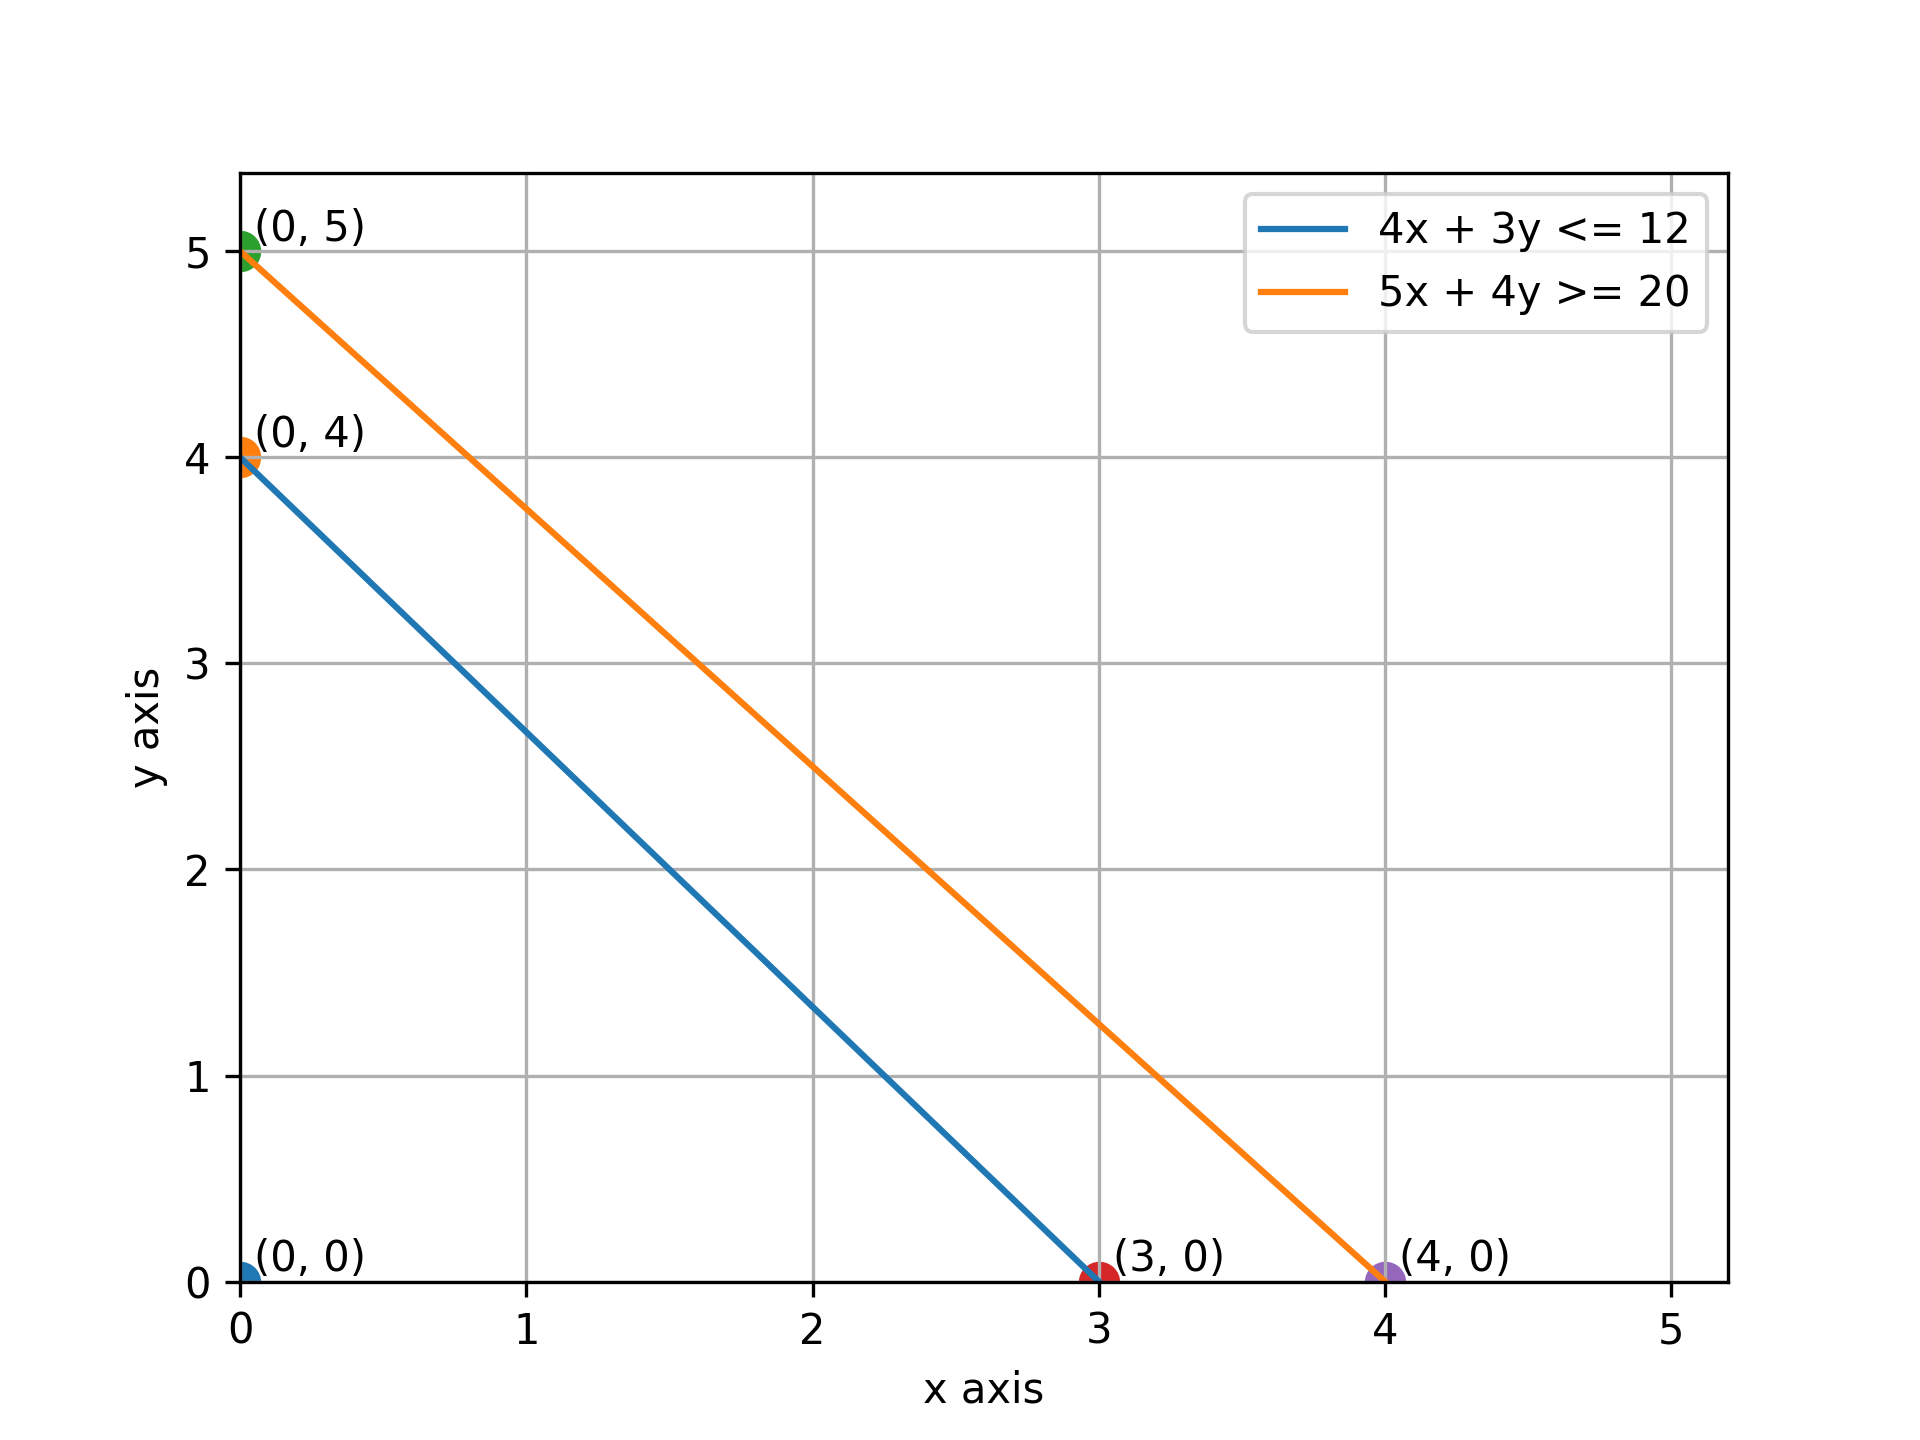
\includegraphics[width=0.6\textwidth]{outputs/graph2.png}
\end{center}
Infeasible Solution\\
\begin{align*}
\text{Maximize} \quad & x + 2y\\
\text{subject to} \quad
& 3x + 2y\le6\\
& 2x + 5y\ge10\\
& x\ge0,\; y\ge0\end{align*}
\begin{align*}
3x + 2y=6\end{align*}
\begin{align*}
2x + 5y=10\end{align*}
Gauss Elimination:\\
Echelon Form:\\
\begin{align*}
\left(
\begin{array}{cc|c}
3 & 2 & 6\\
2 & 5 & 10\\
\end{array}
\right)_{2\times 3}
\end{align*}
\begin{align*}
\left(
\begin{array}{cc|c}
3 & 2 & 6\\
0 & \frac{11}{3} & 6\\
\end{array}
\right)_{2\times 3}
\end{align*}
\begin{align*}
\left(
\begin{array}{cc|c}
3 & 2 & 6\\
0 & \frac{11}{3} & 6\\
\end{array}
\right)_{2\times 3}
\end{align*}
\begin{align*}
x=\frac{10}{11}\end{align*}
\begin{align*}
y=\frac{18}{11}\end{align*}
\begin{center}

\includegraphics[width=0.6\textwidth]{outputs/graph3.png}
\end{center}
\begin{align*}
Z=6\end{align*}
\begin{align*}
x=0\end{align*}
\begin{align*}
y=3\end{align*}
\begin{align*}
\text{Minimize} \quad & 3x - 10y\\
\text{subject to} \quad
& 5x + 2y\ge10\\
& 4x + 3y\le12\\
& x\ge0,\; y\ge0\end{align*}
\begin{align*}
5x + 2y=10\end{align*}
\begin{align*}
4x + 3y=12\end{align*}
Gauss Elimination:\\
Echelon Form:\\
\begin{align*}
\left(
\begin{array}{cc|c}
5 & 2 & 10\\
4 & 3 & 12\\
\end{array}
\right)_{2\times 3}
\end{align*}
\begin{align*}
\left(
\begin{array}{cc|c}
5 & 2 & 10\\
0 & \frac{7}{5} & 4\\
\end{array}
\right)_{2\times 3}
\end{align*}
\begin{align*}
\left(
\begin{array}{cc|c}
5 & 2 & 10\\
0 & \frac{7}{5} & 4\\
\end{array}
\right)_{2\times 3}
\end{align*}
\begin{align*}
x=\frac{6}{7}\end{align*}
\begin{align*}
y=\frac{20}{7}\end{align*}
\begin{center}

\includegraphics[width=0.6\textwidth]{outputs/graph4.png}
\end{center}
\begin{align*}
Z=-26\end{align*}
\begin{align*}
x=6\end{align*}
\begin{align*}
y=20\end{align*}
\begin{align*}
\text{Maximize} \quad & 5x + 4y\\
\text{subject to} \quad
& 2x + 5y\ge10\\
& 3x + 4y\ge12\\
& x\ge0,\; y\ge0\end{align*}
\begin{align*}
2x + 5y=10\end{align*}
\begin{align*}
3x + 4y=12\end{align*}
Gauss Elimination:\\
Echelon Form:\\
\begin{align*}
\left(
\begin{array}{cc|c}
2 & 5 & 10\\
3 & 4 & 12\\
\end{array}
\right)_{2\times 3}
\end{align*}
\begin{align*}
\left(
\begin{array}{cc|c}
2 & 5 & 10\\
0 & -\frac{7}{2} & -3\\
\end{array}
\right)_{2\times 3}
\end{align*}
\begin{align*}
\left(
\begin{array}{cc|c}
2 & 5 & 10\\
0 & -\frac{7}{2} & -3\\
\end{array}
\right)_{2\times 3}
\end{align*}
\begin{align*}
x=\frac{20}{7}\end{align*}
\begin{align*}
y=\frac{6}{7}\end{align*}
\begin{center}

\includegraphics[width=0.6\textwidth]{outputs/graph5.png}
\end{center}
Unbounded Solution\\
\begin{align*}
\text{Minimize} \quad & 5x + 4y\\
\text{subject to} \quad
& 2x + 5y\ge10\\
& 3x + 4y\ge12\\
& x\ge0,\; y\ge0\end{align*}
\begin{align*}
2x + 5y=10\end{align*}
\begin{align*}
3x + 4y=12\end{align*}
Gauss Elimination:\\
Echelon Form:\\
\begin{align*}
\left(
\begin{array}{cc|c}
2 & 5 & 10\\
3 & 4 & 12\\
\end{array}
\right)_{2\times 3}
\end{align*}
\begin{align*}
\left(
\begin{array}{cc|c}
2 & 5 & 10\\
0 & -\frac{7}{2} & -3\\
\end{array}
\right)_{2\times 3}
\end{align*}
\begin{align*}
\left(
\begin{array}{cc|c}
2 & 5 & 10\\
0 & -\frac{7}{2} & -3\\
\end{array}
\right)_{2\times 3}
\end{align*}
\begin{align*}
x=\frac{20}{7}\end{align*}
\begin{align*}
y=\frac{6}{7}\end{align*}
\begin{center}

\includegraphics[width=0.6\textwidth]{outputs/graph6.png}
\end{center}
\begin{align*}
Z=12\end{align*}
\begin{align*}
x=0\end{align*}
\begin{align*}
y=3\end{align*}
\begin{align*}
\text{Maximize} \quad & 10x + 4y\\
\text{subject to} \quad
& 5x + 2y\le100\\
& 3x + 2y\le90\\
& x + 2y\le50\\
& x\ge0,\; y\ge0\end{align*}
\begin{align*}
5x + 2y=100\end{align*}
\begin{align*}
3x + 2y=90\end{align*}
Gauss Elimination:\\
Echelon Form:\\
\begin{align*}
\left(
\begin{array}{cc|c}
5 & 2 & 100\\
3 & 2 & 90\\
\end{array}
\right)_{2\times 3}
\end{align*}
\begin{align*}
\left(
\begin{array}{cc|c}
5 & 2 & 100\\
0 & \frac{4}{5} & 30\\
\end{array}
\right)_{2\times 3}
\end{align*}
\begin{align*}
\left(
\begin{array}{cc|c}
5 & 2 & 100\\
0 & \frac{4}{5} & 30\\
\end{array}
\right)_{2\times 3}
\end{align*}
\begin{align*}
x=5\end{align*}
\begin{align*}
y=\frac{75}{2}\end{align*}
\begin{align*}
5x + 2y=100\end{align*}
\begin{align*}
x + 2y=50\end{align*}
Gauss Elimination:\\
Echelon Form:\\
\begin{align*}
\left(
\begin{array}{cc|c}
5 & 2 & 100\\
1 & 2 & 50\\
\end{array}
\right)_{2\times 3}
\end{align*}
\begin{align*}
\left(
\begin{array}{cc|c}
5 & 2 & 100\\
0 & \frac{8}{5} & 30\\
\end{array}
\right)_{2\times 3}
\end{align*}
\begin{align*}
\left(
\begin{array}{cc|c}
5 & 2 & 100\\
0 & \frac{8}{5} & 30\\
\end{array}
\right)_{2\times 3}
\end{align*}
\begin{align*}
x=\frac{25}{2}\end{align*}
\begin{align*}
y=\frac{75}{4}\end{align*}
\begin{align*}
3x + 2y=90\end{align*}
\begin{align*}
x + 2y=50\end{align*}
Gauss Elimination:\\
Echelon Form:\\
\begin{align*}
\left(
\begin{array}{cc|c}
3 & 2 & 90\\
1 & 2 & 50\\
\end{array}
\right)_{2\times 3}
\end{align*}
\begin{align*}
\left(
\begin{array}{cc|c}
3 & 2 & 90\\
0 & \frac{4}{3} & 20\\
\end{array}
\right)_{2\times 3}
\end{align*}
\begin{align*}
\left(
\begin{array}{cc|c}
3 & 2 & 90\\
0 & \frac{4}{3} & 20\\
\end{array}
\right)_{2\times 3}
\end{align*}
\begin{align*}
x=20\end{align*}
\begin{align*}
y=15\end{align*}
\begin{center}

\includegraphics[width=0.6\textwidth]{outputs/graph7.png}
\end{center}
Infinitely Many Solutions\\
\begin{align*}
\text{Maximize} \quad & 3x + 2y\\
\text{subject to} \quad
& x + y\le4\\
& x - y\le2\\
& x\ge0,\; y\ge0\end{align*}
Standard Form:\\
\begin{align*}
\text{Maximize} \quad & 3x + 2y\\
\text{subject to} \quad
& s_{1} + x + y=4\\
& s_{2} + x - y=2\\
& x\ge0,\; y\ge0\end{align*}
\begin{align*}
\begin{array}{c|c|c|c|c|c|c|c}
 &  &  & 0 & 0 & 3 & 2 & \\
\hline
\text{BV} & \text{C} & \text{B} & s_{1} & s_{2} & x & y & \text{MR} \\
\hline
s_{1} & 0 & 4 & 1 & 0 & 1 & 1 & 4 \\
s_{2} & 0 & 2 & 0 & 1 & 1 & -1 & 2 \\
\hline
 &  & Z_j-C_j & 0 & 0 & -3 & -2 & \\
\end{array}
\end{align*}
\begin{align*}
\begin{array}{c|c|c|c|c|c|c|c}
 &  &  & 0 & 0 & 3 & 2 & \\
\hline
\text{BV} & \text{C} & \text{B} & s_{1} & s_{2} & x & y & \text{MR} \\
\hline
s_{1} & 0 & 2 & 1 & -1 & 0 & 2 & 1 \\
x & 3 & 2 & 0 & 1 & 1 & -1 & - \\
\hline
 &  & Z_j-C_j & 0 & 3 & 0 & -5 & \\
\end{array}
\end{align*}
\begin{align*}
\begin{array}{c|c|c|c|c|c|c|c}
 &  &  & 0 & 0 & 3 & 2 & \\
\hline
\text{BV} & \text{C} & \text{B} & s_{1} & s_{2} & x & y & \text{MR} \\
\hline
y & 2 & 1 & \frac{1}{2} & -\frac{1}{2} & 0 & 1 & 1 \\
x & 3 & 3 & \frac{1}{2} & \frac{1}{2} & 1 & 0 & - \\
\hline
 &  & Z_j-C_j & \frac{5}{2} & \frac{1}{2} & 0 & 0 & \\
\end{array}
\end{align*}
\begin{align*}
\left.3x + 2y\right|_{s_{1}=0,s_{2}=0,x=3,y=1}=11\end{align*}
\begin{align*}
Z=11\end{align*}
\begin{align*}
x=3\end{align*}
\begin{align*}
y=1\end{align*}
\begin{align*}
\text{Maximize} \quad & x_{1} + x_{2} + 3x_{3}\\
\text{subject to} \quad
& 3x_{1} + 2x_{2} + x_{3}\le3\\
& 2x_{1} + x_{2} + 2x_{3}\le2\\
& x_{1}\ge0,\; x_{2}\ge0,\; x_{3}\ge0\end{align*}
Standard Form:\\
\begin{align*}
\text{Maximize} \quad & x_{1} + x_{2} + 3x_{3}\\
\text{subject to} \quad
& s_{1} + 3x_{1} + 2x_{2} + x_{3}=3\\
& s_{2} + 2x_{1} + x_{2} + 2x_{3}=2\\
& x_{1}\ge0,\; x_{2}\ge0,\; x_{3}\ge0\end{align*}
\begin{align*}
\begin{array}{c|c|c|c|c|c|c|c|c}
 &  &  & 0 & 0 & 1 & 1 & 3 & \\
\hline
\text{BV} & \text{C} & \text{B} & s_{1} & s_{2} & x_{1} & x_{2} & x_{3} & \text{MR} \\
\hline
s_{1} & 0 & 3 & 1 & 0 & 3 & 2 & 1 & 3 \\
s_{2} & 0 & 2 & 0 & 1 & 2 & 1 & 2 & 1 \\
\hline
 &  & Z_j-C_j & 0 & 0 & -1 & -1 & -3 & \\
\end{array}
\end{align*}
\begin{align*}
\begin{array}{c|c|c|c|c|c|c|c|c}
 &  &  & 0 & 0 & 1 & 1 & 3 & \\
\hline
\text{BV} & \text{C} & \text{B} & s_{1} & s_{2} & x_{1} & x_{2} & x_{3} & \text{MR} \\
\hline
s_{1} & 0 & 2 & 1 & -\frac{1}{2} & 2 & \frac{3}{2} & 0 & 3 \\
x_{3} & 3 & 1 & 0 & \frac{1}{2} & 1 & \frac{1}{2} & 1 & 1 \\
\hline
 &  & Z_j-C_j & 0 & \frac{3}{2} & 2 & \frac{1}{2} & 0 & \\
\end{array}
\end{align*}
\begin{align*}
\left.x_{1} + x_{2} + 3x_{3}\right|_{s_{1}=0,s_{2}=0,x_{1}=0,x_{2}=0,x_{3}=1}=3\end{align*}
\begin{align*}
Z=3\end{align*}
\begin{align*}
x_{1}=0\end{align*}
\begin{align*}
x_{2}=0\end{align*}
\begin{align*}
x_{3}=1\end{align*}
\begin{align*}
\text{Minimize} \quad & x_{1} - 3x_{2} + 2x_{3}\\
\text{subject to} \quad
& 3x_{1} - x_{2} + 2x_{3}\le7\\
& -2x_{1} + 4x_{2}\le12\\
& -4x_{1} + 3x_{2} + 8x_{3}\le10\\
& x_{1}\ge0,\; x_{2}\ge0,\; x_{3}\ge0\end{align*}
Standard Form:\\
\begin{align*}
\text{Maximize} \quad & -x_{1} + 3x_{2} - 2x_{3}\\
\text{subject to} \quad
& s_{1} + 3x_{1} - x_{2} + 2x_{3}=7\\
& s_{2} - 2x_{1} + 4x_{2}=12\\
& s_{3} - 4x_{1} + 3x_{2} + 8x_{3}=10\\
& x_{1}\ge0,\; x_{2}\ge0,\; x_{3}\ge0\end{align*}
\begin{align*}
\begin{array}{c|c|c|c|c|c|c|c|c|c}
 &  &  & 0 & 0 & 0 & -1 & 3 & -2 & \\
\hline
\text{BV} & \text{C} & \text{B} & s_{1} & s_{2} & s_{3} & x_{1} & x_{2} & x_{3} & \text{MR} \\
\hline
s_{1} & 0 & 7 & 1 & 0 & 0 & 3 & -1 & 2 & - \\
s_{2} & 0 & 12 & 0 & 1 & 0 & -2 & 4 & 0 & 3 \\
s_{3} & 0 & 10 & 0 & 0 & 1 & -4 & 3 & 8 & \frac{10}{3} \\
\hline
 &  & Z_j-C_j & 0 & 0 & 0 & 1 & -3 & 2 & \\
\end{array}
\end{align*}
\begin{align*}
\begin{array}{c|c|c|c|c|c|c|c|c|c}
 &  &  & 0 & 0 & 0 & -1 & 3 & -2 & \\
\hline
\text{BV} & \text{C} & \text{B} & s_{1} & s_{2} & s_{3} & x_{1} & x_{2} & x_{3} & \text{MR} \\
\hline
s_{1} & 0 & 10 & 1 & \frac{1}{4} & 0 & \frac{5}{2} & 0 & 2 & 4 \\
x_{2} & 3 & 3 & 0 & \frac{1}{4} & 0 & -\frac{1}{2} & 1 & 0 & - \\
s_{3} & 0 & 1 & 0 & -\frac{3}{4} & 1 & -\frac{5}{2} & 0 & 8 & - \\
\hline
 &  & Z_j-C_j & 0 & \frac{3}{4} & 0 & -\frac{1}{2} & 0 & 2 & \\
\end{array}
\end{align*}
\begin{align*}
\begin{array}{c|c|c|c|c|c|c|c|c|c}
 &  &  & 0 & 0 & 0 & -1 & 3 & -2 & \\
\hline
\text{BV} & \text{C} & \text{B} & s_{1} & s_{2} & s_{3} & x_{1} & x_{2} & x_{3} & \text{MR} \\
\hline
x_{1} & -1 & 4 & \frac{2}{5} & \frac{1}{10} & 0 & 1 & 0 & \frac{4}{5} & 4 \\
x_{2} & 3 & 5 & \frac{1}{5} & \frac{3}{10} & 0 & 0 & 1 & \frac{2}{5} & - \\
s_{3} & 0 & 11 & 1 & -\frac{1}{2} & 1 & 0 & 0 & 10 & - \\
\hline
 &  & Z_j-C_j & \frac{1}{5} & \frac{4}{5} & 0 & 0 & 0 & \frac{12}{5} & \\
\end{array}
\end{align*}
\begin{align*}
\left.-x_{1} + 3x_{2} - 2x_{3}\right|_{s_{1}=0,s_{2}=0,s_{3}=0,x_{1}=4,x_{2}=5,x_{3}=0}=11\end{align*}
\begin{align*}
Z=-11\end{align*}
\begin{align*}
x_{1}=4\end{align*}
\begin{align*}
x_{2}=5\end{align*}
\begin{align*}
x_{3}=0\end{align*}
\begin{align*}
\text{Maximize} \quad & 2x + y\\
\text{subject to} \quad
& 4x + 3y\le12\\
& 4x + y\le8\\
& 4x - y\le8\\
& x\ge0,\; y\ge0\end{align*}
Standard Form:\\
\begin{align*}
\text{Maximize} \quad & 2x + y\\
\text{subject to} \quad
& s_{1} + 4x + 3y=12\\
& s_{2} + 4x + y=8\\
& s_{3} + 4x - y=8\\
& x\ge0,\; y\ge0\end{align*}
\begin{align*}
\begin{array}{c|c|c|c|c|c|c|c|c}
 &  &  & 0 & 0 & 0 & 2 & 1 & \\
\hline
\text{BV} & \text{C} & \text{B} & s_{1} & s_{2} & s_{3} & x & y & \text{MR} \\
\hline
s_{1} & 0 & 12 & 1 & 0 & 0 & 4 & 3 & 3 \\
s_{2} & 0 & 8 & 0 & 1 & 0 & 4 & 1 & 2 \\
s_{3} & 0 & 8 & 0 & 0 & 1 & 4 & -1 & 2 \\
\hline
 &  & Z_j-C_j & 0 & 0 & 0 & -2 & -1 & \\
\end{array}
\end{align*}
\begin{align*}
\begin{array}{c|c|c|c|c|c|c|c|c}
 &  &  & 0 & 0 & 0 & 2 & 1 & \\
\hline
\text{BV} & \text{C} & \text{B} & s_{1} & s_{2} & s_{3} & x & y & \text{MR} \\
\hline
s_{1} & 0 & 4 & 1 & 0 & -1 & 0 & 4 & 1 \\
s_{2} & 0 & 0 & 0 & 1 & -1 & 0 & 2 & 0 \\
x & 2 & 2 & 0 & 0 & \frac{1}{4} & 1 & -\frac{1}{4} & - \\
\hline
 &  & Z_j-C_j & 0 & 0 & \frac{1}{2} & 0 & -\frac{3}{2} & \\
\end{array}
\end{align*}
\begin{align*}
\begin{array}{c|c|c|c|c|c|c|c|c}
 &  &  & 0 & 0 & 0 & 2 & 1 & \\
\hline
\text{BV} & \text{C} & \text{B} & s_{1} & s_{2} & s_{3} & x & y & \text{MR} \\
\hline
s_{1} & 0 & 4 & 1 & -2 & 1 & 0 & 0 & 4 \\
y & 1 & 0 & 0 & \frac{1}{2} & -\frac{1}{2} & 0 & 1 & - \\
x & 2 & 2 & 0 & \frac{1}{8} & \frac{1}{8} & 1 & 0 & 16 \\
\hline
 &  & Z_j-C_j & 0 & \frac{3}{4} & -\frac{1}{4} & 0 & 0 & \\
\end{array}
\end{align*}
\begin{align*}
\begin{array}{c|c|c|c|c|c|c|c|c}
 &  &  & 0 & 0 & 0 & 2 & 1 & \\
\hline
\text{BV} & \text{C} & \text{B} & s_{1} & s_{2} & s_{3} & x & y & \text{MR} \\
\hline
s_{3} & 0 & 4 & 1 & -2 & 1 & 0 & 0 & 4 \\
y & 1 & 2 & \frac{1}{2} & -\frac{1}{2} & 0 & 0 & 1 & - \\
x & 2 & \frac{3}{2} & -\frac{1}{8} & \frac{3}{8} & 0 & 1 & 0 & 16 \\
\hline
 &  & Z_j-C_j & \frac{1}{4} & \frac{1}{4} & 0 & 0 & 0 & \\
\end{array}
\end{align*}
\begin{align*}
\left.2x + y\right|_{s_{1}=0,s_{2}=0,s_{3}=0,x=\frac{3}{2},y=2}=5\end{align*}
\begin{align*}
Z=5\end{align*}
\begin{align*}
x=\frac{3}{2}\end{align*}
\begin{align*}
y=2\end{align*}
\begin{align*}
\text{Maximize} \quad & 2x + y\\
\text{subject to} \quad
& x - y\le10\\
& 2x - y\le40\\
& x\ge0,\; y\ge0\end{align*}
Standard Form:\\
\begin{align*}
\text{Maximize} \quad & 2x + y\\
\text{subject to} \quad
& s_{1} + x - y=10\\
& s_{2} + 2x - y=40\\
& x\ge0,\; y\ge0\end{align*}
\begin{align*}
\begin{array}{c|c|c|c|c|c|c|c}
 &  &  & 0 & 0 & 2 & 1 & \\
\hline
\text{BV} & \text{C} & \text{B} & s_{1} & s_{2} & x & y & \text{MR} \\
\hline
s_{1} & 0 & 10 & 1 & 0 & 1 & -1 & 10 \\
s_{2} & 0 & 40 & 0 & 1 & 2 & -1 & 20 \\
\hline
 &  & Z_j-C_j & 0 & 0 & -2 & -1 & \\
\end{array}
\end{align*}
\begin{align*}
\begin{array}{c|c|c|c|c|c|c|c}
 &  &  & 0 & 0 & 2 & 1 & \\
\hline
\text{BV} & \text{C} & \text{B} & s_{1} & s_{2} & x & y & \text{MR} \\
\hline
x & 2 & 10 & 1 & 0 & 1 & -1 & - \\
s_{2} & 0 & 20 & -2 & 1 & 0 & 1 & 20 \\
\hline
 &  & Z_j-C_j & 2 & 0 & 0 & -3 & \\
\end{array}
\end{align*}
\begin{align*}
\begin{array}{c|c|c|c|c|c|c|c}
 &  &  & 0 & 0 & 2 & 1 & \\
\hline
\text{BV} & \text{C} & \text{B} & s_{1} & s_{2} & x & y & \text{MR} \\
\hline
x & 2 & 30 & -1 & 1 & 1 & 0 & - \\
y & 1 & 20 & -2 & 1 & 0 & 1 & - \\
\hline
 &  & Z_j-C_j & -4 & 3 & 0 & 0 & \\
\end{array}
\end{align*}
Unbounded Solution\\
\begin{align*}
\text{Maximize} \quad & 3x + 2y\\
\text{subject to} \quad
& x - y\le1\\
& 3x - 2y\le6\\
& x\ge0,\; y\ge0\end{align*}
Standard Form:\\
\begin{align*}
\text{Maximize} \quad & 3x + 2y\\
\text{subject to} \quad
& s_{1} + x - y=1\\
& s_{2} + 3x - 2y=6\\
& x\ge0,\; y\ge0\end{align*}
\begin{align*}
\begin{array}{c|c|c|c|c|c|c|c}
 &  &  & 0 & 0 & 3 & 2 & \\
\hline
\text{BV} & \text{C} & \text{B} & s_{1} & s_{2} & x & y & \text{MR} \\
\hline
s_{1} & 0 & 1 & 1 & 0 & 1 & -1 & 1 \\
s_{2} & 0 & 6 & 0 & 1 & 3 & -2 & 2 \\
\hline
 &  & Z_j-C_j & 0 & 0 & -3 & -2 & \\
\end{array}
\end{align*}
\begin{align*}
\begin{array}{c|c|c|c|c|c|c|c}
 &  &  & 0 & 0 & 3 & 2 & \\
\hline
\text{BV} & \text{C} & \text{B} & s_{1} & s_{2} & x & y & \text{MR} \\
\hline
x & 3 & 1 & 1 & 0 & 1 & -1 & - \\
s_{2} & 0 & 3 & -3 & 1 & 0 & 1 & 3 \\
\hline
 &  & Z_j-C_j & 3 & 0 & 0 & -5 & \\
\end{array}
\end{align*}
\begin{align*}
\begin{array}{c|c|c|c|c|c|c|c}
 &  &  & 0 & 0 & 3 & 2 & \\
\hline
\text{BV} & \text{C} & \text{B} & s_{1} & s_{2} & x & y & \text{MR} \\
\hline
x & 3 & 4 & -2 & 1 & 1 & 0 & - \\
y & 2 & 3 & -3 & 1 & 0 & 1 & - \\
\hline
 &  & Z_j-C_j & -12 & 5 & 0 & 0 & \\
\end{array}
\end{align*}
Unbounded Solution\\
\begin{align*}
\text{Maximize} \quad & x_{1} + 2x_{2} + x_{3}\\
\text{subject to} \quad
& 2x_{1} + x_{2} - x_{3}\ge-2\\
& -2x_{1} + x_{2} - 5x_{3}\le6\\
& 4x_{1} + x_{2} + x_{3}\le6\\
& x_{1}\ge0,\; x_{2}\ge0,\; x_{3}\ge0\end{align*}
Standard Form:\\
\begin{align*}
\text{Maximize} \quad & x_{1} + 2x_{2} + x_{3}\\
\text{subject to} \quad
& s_{1} - 2x_{1} - x_{2} + x_{3}=2\\
& s_{2} - 2x_{1} + x_{2} - 5x_{3}=6\\
& s_{3} + 4x_{1} + x_{2} + x_{3}=6\\
& x_{1}\ge0,\; x_{2}\ge0,\; x_{3}\ge0\end{align*}
\begin{align*}
\begin{array}{c|c|c|c|c|c|c|c|c|c}
 &  &  & 0 & 0 & 0 & 1 & 2 & 1 & \\
\hline
\text{BV} & \text{C} & \text{B} & s_{1} & s_{2} & s_{3} & x_{1} & x_{2} & x_{3} & \text{MR} \\
\hline
s_{1} & 0 & 2 & 1 & 0 & 0 & -2 & -1 & 1 & - \\
s_{2} & 0 & 6 & 0 & 1 & 0 & -2 & 1 & -5 & 6 \\
s_{3} & 0 & 6 & 0 & 0 & 1 & 4 & 1 & 1 & 6 \\
\hline
 &  & Z_j-C_j & 0 & 0 & 0 & -1 & -2 & -1 & \\
\end{array}
\end{align*}
\begin{align*}
\begin{array}{c|c|c|c|c|c|c|c|c|c}
 &  &  & 0 & 0 & 0 & 1 & 2 & 1 & \\
\hline
\text{BV} & \text{C} & \text{B} & s_{1} & s_{2} & s_{3} & x_{1} & x_{2} & x_{3} & \text{MR} \\
\hline
s_{1} & 0 & 8 & 1 & 0 & 1 & 2 & 0 & 2 & - \\
s_{2} & 0 & 0 & 0 & 1 & -1 & -6 & 0 & -6 & 1 \\
x_{2} & 2 & 6 & 0 & 0 & 1 & 4 & 1 & 1 & 0 \\
\hline
 &  & Z_j-C_j & 0 & 0 & 2 & 7 & 0 & 1 & \\
\end{array}
\end{align*}
\begin{align*}
\left.x_{1} + 2x_{2} + x_{3}\right|_{s_{1}=0,s_{2}=0,s_{3}=0,x_{1}=0,x_{2}=6,x_{3}=0}=12\end{align*}
\begin{align*}
Z=12\end{align*}
\begin{align*}
x_{1}=0\end{align*}
\begin{align*}
x_{2}=6\end{align*}
\begin{align*}
x_{3}=0\end{align*}
\begin{align*}
\text{Maximize} \quad & -4x_{1} - x_{2}\\
\text{subject to} \quad
& 3x_{1} + x_{2}=3\\
& 4x_{1} + 3x_{2}\ge6\\
& x_{1} + 2x_{2}\le3\\
& x_{1}\ge0,\; x_{2}\ge0\end{align*}
Standard Form:\\
\begin{align*}
\text{Maximize} \quad & -4x_{1} - x_{2}\\
\text{subject to} \quad
& 3x_{1} + x_{2}=3\\
& -s_{1} + 4x_{1} + 3x_{2}=6\\
& s_{2} + x_{1} + 2x_{2}=3\\
& x_{1}\ge0,\; x_{2}\ge0\end{align*}
\begin{align*}
\begin{array}{c|c|c|c|c|c|c|c|c|c}
 &  &  & -M & -M & 0 & 0 & -4 & -1 & \\
\hline
\text{BV} & \text{C} & \text{B} & A_{1} & A_{2} & s_{1} & s_{2} & x_{1} & x_{2} & \text{MR} \\
\hline
A_{1} & -M & 3 & 1 & 0 & 0 & 0 & 3 & 1 & 1 \\
A_{2} & -M & 6 & 0 & 1 & -1 & 0 & 4 & 3 & \frac{3}{2} \\
s_{2} & 0 & 3 & 0 & 0 & 0 & 1 & 1 & 2 & 3 \\
\hline
 &  & Z_j-C_j & 0 & 0 & M & 0 & -7M + 4 & -4M + 1 & \\
\end{array}
\end{align*}
\begin{align*}
\begin{array}{c|c|c|c|c|c|c|c|c}
 &  &  & -M & 0 & 0 & -4 & -1 & \\
\hline
\text{BV} & \text{C} & \text{B} & A_{2} & s_{1} & s_{2} & x_{1} & x_{2} & \text{MR} \\
\hline
x_{1} & -4 & 1 & 0 & 0 & 0 & 1 & \frac{1}{3} & 3 \\
A_{2} & -M & 2 & 1 & -1 & 0 & 0 & \frac{5}{3} & \frac{6}{5} \\
s_{2} & 0 & 2 & 0 & 0 & 1 & 0 & \frac{5}{3} & \frac{6}{5} \\
\hline
 &  & Z_j-C_j & 0 & M & 0 & 0 & \dfrac{-5M}{3} - \frac{1}{3} & \\
\end{array}
\end{align*}
\begin{align*}
\begin{array}{c|c|c|c|c|c|c|c}
 &  &  & 0 & 0 & -4 & -1 & \\
\hline
\text{BV} & \text{C} & \text{B} & s_{1} & s_{2} & x_{1} & x_{2} & \text{MR} \\
\hline
x_{1} & -4 & \frac{3}{5} & \frac{1}{5} & 0 & 1 & 0 & 3 \\
x_{2} & -1 & \frac{6}{5} & -\frac{3}{5} & 0 & 0 & 1 & - \\
s_{2} & 0 & 0 & 1 & 1 & 0 & 0 & 0 \\
\hline
 &  & Z_j-C_j & -\frac{1}{5} & 0 & 0 & 0 & \\
\end{array}
\end{align*}
\begin{align*}
\begin{array}{c|c|c|c|c|c|c|c}
 &  &  & 0 & 0 & -4 & -1 & \\
\hline
\text{BV} & \text{C} & \text{B} & s_{1} & s_{2} & x_{1} & x_{2} & \text{MR} \\
\hline
x_{1} & -4 & \frac{3}{5} & 0 & -\frac{1}{5} & 1 & 0 & 3 \\
x_{2} & -1 & \frac{6}{5} & 0 & \frac{3}{5} & 0 & 1 & - \\
s_{1} & 0 & 0 & 1 & 1 & 0 & 0 & 0 \\
\hline
 &  & Z_j-C_j & 0 & \frac{1}{5} & 0 & 0 & \\
\end{array}
\end{align*}
\begin{align*}
\left.-4x_{1} - x_{2}\right|_{s_{1}=0,s_{2}=0,x_{1}=\frac{3}{5},x_{2}=\frac{6}{5}}=-\frac{18}{5}\end{align*}
\begin{align*}
Z=-\frac{18}{5}\end{align*}
\begin{align*}
x_{1}=\frac{3}{5}\end{align*}
\begin{align*}
x_{2}=\frac{6}{5}\end{align*}
\begin{align*}
\text{Maximize} \quad & -x - y\\
\text{subject to} \quad
& 3x + 2y\ge30\\
& -2x + 3y\le-30\\
& x + y\le5\\
& x\ge0,\; y\ge0\end{align*}
Standard Form:\\
\begin{align*}
\text{Maximize} \quad & -x - y\\
\text{subject to} \quad
& -s_{1} + 3x + 2y=30\\
& -s_{2} + 2x - 3y=30\\
& s_{3} + x + y=5\\
& x\ge0,\; y\ge0\end{align*}
\begin{align*}
\begin{array}{c|c|c|c|c|c|c|c|c|c|c}
 &  &  & -M & -M & 0 & 0 & 0 & -1 & -1 & \\
\hline
\text{BV} & \text{C} & \text{B} & A_{1} & A_{2} & s_{1} & s_{2} & s_{3} & x & y & \text{MR} \\
\hline
A_{1} & -M & 30 & 1 & 0 & -1 & 0 & 0 & 3 & 2 & 10 \\
A_{2} & -M & 30 & 0 & 1 & 0 & -1 & 0 & 2 & -3 & 15 \\
s_{3} & 0 & 5 & 0 & 0 & 0 & 0 & 1 & 1 & 1 & 5 \\
\hline
 &  & Z_j-C_j & 0 & 0 & M & M & 0 & -5M + 1 & M + 1 & \\
\end{array}
\end{align*}
Infeasible Solution\\
\begin{align*}
\text{Maximize} \quad & -4x - y\\
\text{subject to} \quad
& 3x + y=3\\
& 4x + 3y\ge6\\
& x + 2y\le3\\
& x\ge0,\; y\ge0\end{align*}
Standard Form:\\
\begin{align*}
\text{Maximize} \quad & -4x - y\\
\text{subject to} \quad
& 3x + y=3\\
& -s_{1} + 4x + 3y=6\\
& s_{2} + x + 2y=3\\
& x\ge0,\; y\ge0\end{align*}
\begin{align*}
\begin{array}{c|c|c|c|c|c|c|c|c|c}
 &  &  & -1 & -1 & 0 & 0 & 0 & 0 & \\
\hline
\text{BV} & \text{C} & \text{B} & A_{1} & A_{2} & s_{1} & s_{2} & x & y & \text{MR} \\
\hline
A_{1} & -1 & 3 & 1 & 0 & 0 & 0 & 3 & 1 & 1 \\
A_{2} & -1 & 6 & 0 & 1 & -1 & 0 & 4 & 3 & \frac{3}{2} \\
s_{2} & 0 & 3 & 0 & 0 & 0 & 1 & 1 & 2 & 3 \\
\hline
 &  & Z_j-C_j & 0 & 0 & 1 & 0 & -7 & -4 & \\
\end{array}
\end{align*}
\begin{align*}
\begin{array}{c|c|c|c|c|c|c|c|c}
 &  &  & -1 & 0 & 0 & 0 & 0 & \\
\hline
\text{BV} & \text{C} & \text{B} & A_{2} & s_{1} & s_{2} & x & y & \text{MR} \\
\hline
x & 0 & 1 & 0 & 0 & 0 & 1 & \frac{1}{3} & 3 \\
A_{2} & -1 & 2 & 1 & -1 & 0 & 0 & \frac{5}{3} & \frac{6}{5} \\
s_{2} & 0 & 2 & 0 & 0 & 1 & 0 & \frac{5}{3} & \frac{6}{5} \\
\hline
 &  & Z_j-C_j & 0 & 1 & 0 & 0 & -\frac{5}{3} & \\
\end{array}
\end{align*}
\begin{align*}
\begin{array}{c|c|c|c|c|c|c|c}
 &  &  & 0 & 0 & -4 & -1 & \\
\hline
\text{BV} & \text{C} & \text{B} & s_{1} & s_{2} & x & y & \text{MR} \\
\hline
x & -4 & \frac{3}{5} & \frac{1}{5} & 0 & 1 & 0 & 3 \\
y & -1 & \frac{6}{5} & -\frac{3}{5} & 0 & 0 & 1 & - \\
s_{2} & 0 & 0 & 1 & 1 & 0 & 0 & 0 \\
\hline
 &  & Z_j-C_j & -\frac{1}{5} & 0 & 0 & 0 & \\
\end{array}
\end{align*}
\begin{align*}
\begin{array}{c|c|c|c|c|c|c|c}
 &  &  & 0 & 0 & -4 & -1 & \\
\hline
\text{BV} & \text{C} & \text{B} & s_{1} & s_{2} & x & y & \text{MR} \\
\hline
x & -4 & \frac{3}{5} & 0 & -\frac{1}{5} & 1 & 0 & 3 \\
y & -1 & \frac{6}{5} & 0 & \frac{3}{5} & 0 & 1 & - \\
s_{1} & 0 & 0 & 1 & 1 & 0 & 0 & 0 \\
\hline
 &  & Z_j-C_j & 0 & \frac{1}{5} & 0 & 0 & \\
\end{array}
\end{align*}
\begin{align*}
\left.-4x - y\right|_{s_{1}=0,s_{2}=0,x=\frac{3}{5},y=\frac{6}{5}}=-\frac{18}{5}\end{align*}
\begin{align*}
Z=-\frac{18}{5}\end{align*}
\begin{align*}
x=\frac{3}{5}\end{align*}
\begin{align*}
y=\frac{6}{5}\end{align*}
\begin{align*}
\text{Maximize} \quad & 3x_{1} + 2x_{2} + x_{3}\\
\text{subject to} \quad
& -3x_{1} + 2x_{2} + 2x_{3}=8\\
& -3x_{1} + 4x_{2} + x_{3}=7\\
& x_{1}\ge0,\; x_{2}\ge0,\; x_{3}\ge0\end{align*}
Standard Form:\\
\begin{align*}
\text{Maximize} \quad & 3x_{1} + 2x_{2} + x_{3}\\
\text{subject to} \quad
& -3x_{1} + 2x_{2} + 2x_{3}=8\\
& -3x_{1} + 4x_{2} + x_{3}=7\\
& x_{1}\ge0,\; x_{2}\ge0,\; x_{3}\ge0\end{align*}
\begin{align*}
\begin{array}{c|c|c|c|c|c|c|c|c}
 &  &  & -M & -M & 3 & 2 & 1 & \\
\hline
\text{BV} & \text{C} & \text{B} & A_{1} & A_{2} & x_{1} & x_{2} & x_{3} & \text{MR} \\
\hline
A_{1} & -M & 8 & 1 & 0 & -3 & 2 & 2 & 4 \\
A_{2} & -M & 7 & 0 & 1 & -3 & 4 & 1 & \frac{7}{4} \\
\hline
 &  & Z_j-C_j & 0 & 0 & 6M - 3 & -6M - 2 & -3M - 1 & \\
\end{array}
\end{align*}
\begin{align*}
\begin{array}{c|c|c|c|c|c|c|c}
 &  &  & -M & 3 & 2 & 1 & \\
\hline
\text{BV} & \text{C} & \text{B} & A_{1} & x_{1} & x_{2} & x_{3} & \text{MR} \\
\hline
A_{1} & -M & \frac{9}{2} & 1 & -\frac{3}{2} & 0 & \frac{3}{2} & 3 \\
x_{2} & 2 & \frac{7}{4} & 0 & -\frac{3}{4} & 1 & \frac{1}{4} & 7 \\
\hline
 &  & Z_j-C_j & 0 & \dfrac{3M}{2} - \frac{9}{2} & 0 & \dfrac{-3M}{2} - \frac{1}{2} & \\
\end{array}
\end{align*}
\begin{align*}
\begin{array}{c|c|c|c|c|c|c}
 &  &  & 3 & 2 & 1 & \\
\hline
\text{BV} & \text{C} & \text{B} & x_{1} & x_{2} & x_{3} & \text{MR} \\
\hline
x_{3} & 1 & 3 & -1 & 0 & 1 & - \\
x_{2} & 2 & 1 & -\frac{1}{2} & 1 & 0 & - \\
\hline
 &  & Z_j-C_j & -5 & 0 & 0 & \\
\end{array}
\end{align*}
Unbounded Solution\\
\begin{align*}
x_{1} + 2x_{2} + x_{3}=4\end{align*}
\begin{align*}
2x_{1} + x_{2} + 5x_{3}=5\end{align*}
Determinant:\\
Echelon Form:\\
\begin{align*}
\begin{vmatrix}
1 & 2\\
2 & 1\\
\end{vmatrix}_{2\times 2}
\end{align*}
\begin{align*}
\begin{vmatrix}
1 & 2\\
0 & -3\\
\end{vmatrix}_{2\times 2}
\end{align*}
\begin{align*}
\begin{vmatrix}
1 & 2\\
0 & -3\\
\end{vmatrix}_{2\times 2}
\end{align*}
Inverse:\\
\begin{align*}
\begin{pmatrix}
1 & 2\\
2 & 1\\
\end{pmatrix}_{2\times 2}
\end{align*}
\begin{align*}
\left(
\begin{array}{cc|cc}
1 & 2 & 1 & 0\\
2 & 1 & 0 & 1\\
\end{array}
\right)_{2\times 4}
\end{align*}
Echelon Form:\\
\begin{align*}
\left(
\begin{array}{cc|cc}
1 & 2 & 1 & 0\\
2 & 1 & 0 & 1\\
\end{array}
\right)_{2\times 4}
\end{align*}
\begin{align*}
\left(
\begin{array}{cc|cc}
1 & 2 & 1 & 0\\
0 & -3 & -2 & 1\\
\end{array}
\right)_{2\times 4}
\end{align*}
\begin{align*}
\left(
\begin{array}{cc|cc}
1 & 2 & 1 & 0\\
0 & -3 & -2 & 1\\
\end{array}
\right)_{2\times 4}
\end{align*}
\begin{align*}
\left(
\begin{array}{cc|cc}
1 & 0 & -\frac{1}{3} & \frac{2}{3}\\
0 & 1 & \frac{2}{3} & -\frac{1}{3}\\
\end{array}
\right)_{2\times 4}
\end{align*}
\begin{align*}
\left(
\begin{array}{cc|cc}
1 & 0 & -\frac{1}{3} & \frac{2}{3}\\
0 & 1 & \frac{2}{3} & -\frac{1}{3}\\
\end{array}
\right)_{2\times 4}
\end{align*}
Determinant:\\
Echelon Form:\\
\begin{align*}
\begin{vmatrix}
1 & 1\\
2 & 5\\
\end{vmatrix}_{2\times 2}
\end{align*}
\begin{align*}
\begin{vmatrix}
1 & 1\\
0 & 3\\
\end{vmatrix}_{2\times 2}
\end{align*}
\begin{align*}
\begin{vmatrix}
1 & 1\\
0 & 3\\
\end{vmatrix}_{2\times 2}
\end{align*}
Inverse:\\
\begin{align*}
\begin{pmatrix}
1 & 1\\
2 & 5\\
\end{pmatrix}_{2\times 2}
\end{align*}
\begin{align*}
\left(
\begin{array}{cc|cc}
1 & 1 & 1 & 0\\
2 & 5 & 0 & 1\\
\end{array}
\right)_{2\times 4}
\end{align*}
Echelon Form:\\
\begin{align*}
\left(
\begin{array}{cc|cc}
1 & 1 & 1 & 0\\
2 & 5 & 0 & 1\\
\end{array}
\right)_{2\times 4}
\end{align*}
\begin{align*}
\left(
\begin{array}{cc|cc}
1 & 1 & 1 & 0\\
0 & 3 & -2 & 1\\
\end{array}
\right)_{2\times 4}
\end{align*}
\begin{align*}
\left(
\begin{array}{cc|cc}
1 & 1 & 1 & 0\\
0 & 3 & -2 & 1\\
\end{array}
\right)_{2\times 4}
\end{align*}
\begin{align*}
\left(
\begin{array}{cc|cc}
1 & 0 & \frac{5}{3} & -\frac{1}{3}\\
0 & 1 & -\frac{2}{3} & \frac{1}{3}\\
\end{array}
\right)_{2\times 4}
\end{align*}
\begin{align*}
\left(
\begin{array}{cc|cc}
1 & 0 & \frac{5}{3} & -\frac{1}{3}\\
0 & 1 & -\frac{2}{3} & \frac{1}{3}\\
\end{array}
\right)_{2\times 4}
\end{align*}
Determinant:\\
Echelon Form:\\
\begin{align*}
\begin{vmatrix}
2 & 1\\
1 & 5\\
\end{vmatrix}_{2\times 2}
\end{align*}
\begin{align*}
\begin{vmatrix}
2 & 1\\
0 & \frac{9}{2}\\
\end{vmatrix}_{2\times 2}
\end{align*}
\begin{align*}
\begin{vmatrix}
2 & 1\\
0 & \frac{9}{2}\\
\end{vmatrix}_{2\times 2}
\end{align*}
Inverse:\\
\begin{align*}
\begin{pmatrix}
2 & 1\\
1 & 5\\
\end{pmatrix}_{2\times 2}
\end{align*}
\begin{align*}
\left(
\begin{array}{cc|cc}
2 & 1 & 1 & 0\\
1 & 5 & 0 & 1\\
\end{array}
\right)_{2\times 4}
\end{align*}
Echelon Form:\\
\begin{align*}
\left(
\begin{array}{cc|cc}
2 & 1 & 1 & 0\\
1 & 5 & 0 & 1\\
\end{array}
\right)_{2\times 4}
\end{align*}
\begin{align*}
\left(
\begin{array}{cc|cc}
2 & 1 & 1 & 0\\
0 & \frac{9}{2} & -\frac{1}{2} & 1\\
\end{array}
\right)_{2\times 4}
\end{align*}
\begin{align*}
\left(
\begin{array}{cc|cc}
2 & 1 & 1 & 0\\
0 & \frac{9}{2} & -\frac{1}{2} & 1\\
\end{array}
\right)_{2\times 4}
\end{align*}
\begin{align*}
\left(
\begin{array}{cc|cc}
2 & 0 & \frac{10}{9} & -\frac{2}{9}\\
0 & 1 & -\frac{1}{9} & \frac{2}{9}\\
\end{array}
\right)_{2\times 4}
\end{align*}
\begin{align*}
\left(
\begin{array}{cc|cc}
1 & 0 & \frac{5}{9} & -\frac{1}{9}\\
0 & 1 & -\frac{1}{9} & \frac{2}{9}\\
\end{array}
\right)_{2\times 4}
\end{align*}
Basic Feasible Solutions:\\
\begin{align*}
x_{1}=2\end{align*}
  \begin{align*}
x_{2}=1\end{align*}
  \\
\begin{align*}
x_{1}=5\end{align*}
  \begin{align*}
x_{3}=-1\end{align*}
  \\
\begin{align*}
x_{2}=\frac{5}{3}\end{align*}
  \begin{align*}
x_{3}=\frac{2}{3}\end{align*}
  \\
\begin{align*}
2x_{1} + x_{2} - x_{3}=2\end{align*}
\begin{align*}
3x_{1} + 2x_{2} + x_{3}=3\end{align*}
Determinant:\\
Echelon Form:\\
\begin{align*}
\begin{vmatrix}
2 & 1\\
3 & 2\\
\end{vmatrix}_{2\times 2}
\end{align*}
\begin{align*}
\begin{vmatrix}
2 & 1\\
0 & \frac{1}{2}\\
\end{vmatrix}_{2\times 2}
\end{align*}
\begin{align*}
\begin{vmatrix}
2 & 1\\
0 & \frac{1}{2}\\
\end{vmatrix}_{2\times 2}
\end{align*}
Inverse:\\
\begin{align*}
\begin{pmatrix}
2 & 1\\
3 & 2\\
\end{pmatrix}_{2\times 2}
\end{align*}
\begin{align*}
\left(
\begin{array}{cc|cc}
2 & 1 & 1 & 0\\
3 & 2 & 0 & 1\\
\end{array}
\right)_{2\times 4}
\end{align*}
Echelon Form:\\
\begin{align*}
\left(
\begin{array}{cc|cc}
2 & 1 & 1 & 0\\
3 & 2 & 0 & 1\\
\end{array}
\right)_{2\times 4}
\end{align*}
\begin{align*}
\left(
\begin{array}{cc|cc}
2 & 1 & 1 & 0\\
0 & \frac{1}{2} & -\frac{3}{2} & 1\\
\end{array}
\right)_{2\times 4}
\end{align*}
\begin{align*}
\left(
\begin{array}{cc|cc}
2 & 1 & 1 & 0\\
0 & \frac{1}{2} & -\frac{3}{2} & 1\\
\end{array}
\right)_{2\times 4}
\end{align*}
\begin{align*}
\left(
\begin{array}{cc|cc}
2 & 0 & 4 & -2\\
0 & 1 & -3 & 2\\
\end{array}
\right)_{2\times 4}
\end{align*}
\begin{align*}
\left(
\begin{array}{cc|cc}
1 & 0 & 2 & -1\\
0 & 1 & -3 & 2\\
\end{array}
\right)_{2\times 4}
\end{align*}
Determinant:\\
Echelon Form:\\
\begin{align*}
\begin{vmatrix}
2 & -1\\
3 & 1\\
\end{vmatrix}_{2\times 2}
\end{align*}
\begin{align*}
\begin{vmatrix}
2 & -1\\
0 & \frac{5}{2}\\
\end{vmatrix}_{2\times 2}
\end{align*}
\begin{align*}
\begin{vmatrix}
2 & -1\\
0 & \frac{5}{2}\\
\end{vmatrix}_{2\times 2}
\end{align*}
Inverse:\\
\begin{align*}
\begin{pmatrix}
2 & -1\\
3 & 1\\
\end{pmatrix}_{2\times 2}
\end{align*}
\begin{align*}
\left(
\begin{array}{cc|cc}
2 & -1 & 1 & 0\\
3 & 1 & 0 & 1\\
\end{array}
\right)_{2\times 4}
\end{align*}
Echelon Form:\\
\begin{align*}
\left(
\begin{array}{cc|cc}
2 & -1 & 1 & 0\\
3 & 1 & 0 & 1\\
\end{array}
\right)_{2\times 4}
\end{align*}
\begin{align*}
\left(
\begin{array}{cc|cc}
2 & -1 & 1 & 0\\
0 & \frac{5}{2} & -\frac{3}{2} & 1\\
\end{array}
\right)_{2\times 4}
\end{align*}
\begin{align*}
\left(
\begin{array}{cc|cc}
2 & -1 & 1 & 0\\
0 & \frac{5}{2} & -\frac{3}{2} & 1\\
\end{array}
\right)_{2\times 4}
\end{align*}
\begin{align*}
\left(
\begin{array}{cc|cc}
2 & 0 & \frac{2}{5} & \frac{2}{5}\\
0 & 1 & -\frac{3}{5} & \frac{2}{5}\\
\end{array}
\right)_{2\times 4}
\end{align*}
\begin{align*}
\left(
\begin{array}{cc|cc}
1 & 0 & \frac{1}{5} & \frac{1}{5}\\
0 & 1 & -\frac{3}{5} & \frac{2}{5}\\
\end{array}
\right)_{2\times 4}
\end{align*}
Determinant:\\
Echelon Form:\\
\begin{align*}
\begin{vmatrix}
1 & -1\\
2 & 1\\
\end{vmatrix}_{2\times 2}
\end{align*}
\begin{align*}
\begin{vmatrix}
1 & -1\\
0 & 3\\
\end{vmatrix}_{2\times 2}
\end{align*}
\begin{align*}
\begin{vmatrix}
1 & -1\\
0 & 3\\
\end{vmatrix}_{2\times 2}
\end{align*}
Inverse:\\
\begin{align*}
\begin{pmatrix}
1 & -1\\
2 & 1\\
\end{pmatrix}_{2\times 2}
\end{align*}
\begin{align*}
\left(
\begin{array}{cc|cc}
1 & -1 & 1 & 0\\
2 & 1 & 0 & 1\\
\end{array}
\right)_{2\times 4}
\end{align*}
Echelon Form:\\
\begin{align*}
\left(
\begin{array}{cc|cc}
1 & -1 & 1 & 0\\
2 & 1 & 0 & 1\\
\end{array}
\right)_{2\times 4}
\end{align*}
\begin{align*}
\left(
\begin{array}{cc|cc}
1 & -1 & 1 & 0\\
0 & 3 & -2 & 1\\
\end{array}
\right)_{2\times 4}
\end{align*}
\begin{align*}
\left(
\begin{array}{cc|cc}
1 & -1 & 1 & 0\\
0 & 3 & -2 & 1\\
\end{array}
\right)_{2\times 4}
\end{align*}
\begin{align*}
\left(
\begin{array}{cc|cc}
1 & 0 & \frac{1}{3} & \frac{1}{3}\\
0 & 1 & -\frac{2}{3} & \frac{1}{3}\\
\end{array}
\right)_{2\times 4}
\end{align*}
\begin{align*}
\left(
\begin{array}{cc|cc}
1 & 0 & \frac{1}{3} & \frac{1}{3}\\
0 & 1 & -\frac{2}{3} & \frac{1}{3}\\
\end{array}
\right)_{2\times 4}
\end{align*}
Basic Feasible Solutions:\\
\begin{align*}
x_{1}=1\end{align*}
  \begin{align*}
x_{2}=0\end{align*}
  \\
\begin{align*}
x_{1}=1\end{align*}
  \begin{align*}
x_{3}=0\end{align*}
  \\
\begin{align*}
x_{2}=\frac{5}{3}\end{align*}
  \begin{align*}
x_{3}=-\frac{1}{3}\end{align*}
  \\
\begin{align*}
\text{Maximize} \quad & 2x_{1} + 3x_{2} + 10x_{3}\\
\text{subject to} \quad
& x_{1} + 2x_{3}=0\\
& x_{2} + x_{3}=1\\
& x_{1}\ge0,\; x_{2}\ge0,\; x_{3}\ge0\end{align*}
Standard Form:\\
\begin{align*}
\text{Maximize} \quad & 2x_{1} + 3x_{2} + 10x_{3}\\
\text{subject to} \quad
& x_{1} + 2x_{3}=0\\
& x_{2} + x_{3}=1\\
& x_{1}\ge0,\; x_{2}\ge0,\; x_{3}\ge0\end{align*}
\begin{align*}
\begin{array}{c|c|c|c|c|c|c}
 &  &  & 2 & 3 & 10 & \\
\hline
\text{BV} & \text{C} & \text{B} & x_{1} & x_{2} & x_{3} & \text{MR} \\
\hline
x_{1} & 2 & 0 & 1 & 0 & 2 & 0 \\
x_{2} & 3 & 1 & 0 & 1 & 1 & 1 \\
\hline
 &  & Z_j-C_j & 0 & 0 & -3 & \\
\end{array}
\end{align*}
\begin{align*}
\begin{array}{c|c|c|c|c|c|c}
 &  &  & 2 & 3 & 10 & \\
\hline
\text{BV} & \text{C} & \text{B} & x_{1} & x_{2} & x_{3} & \text{MR} \\
\hline
x_{3} & 10 & 0 & \frac{1}{2} & 0 & 1 & 0 \\
x_{2} & 3 & 1 & -\frac{1}{2} & 1 & 0 & 1 \\
\hline
 &  & Z_j-C_j & \frac{3}{2} & 0 & 0 & \\
\end{array}
\end{align*}
\begin{align*}
\left.2x_{1} + 3x_{2} + 10x_{3}\right|_{x_{1}=0,x_{2}=1,x_{3}=0}=3\end{align*}
\begin{align*}
Z=3\end{align*}
\begin{align*}
x_{1}=0\end{align*}
\begin{align*}
x_{2}=1\end{align*}
\begin{align*}
x_{3}=0\end{align*}
\begin{align*}
\text{Maximize} \quad & 2x_{1} + 3x_{2} + 10x_{3}\\
\text{subject to} \quad
& x_{1} - 2x_{3}=0\\
& x_{2} + x_{3}=1\\
& x_{1}\ge0,\; x_{2}\ge0,\; x_{3}\ge0\end{align*}
Standard Form:\\
\begin{align*}
\text{Maximize} \quad & 2x_{1} + 3x_{2} + 10x_{3}\\
\text{subject to} \quad
& x_{1} - 2x_{3}=0\\
& x_{2} + x_{3}=1\\
& x_{1}\ge0,\; x_{2}\ge0,\; x_{3}\ge0\end{align*}
\begin{align*}
\begin{array}{c|c|c|c|c|c|c}
 &  &  & 2 & 3 & 10 & \\
\hline
\text{BV} & \text{C} & \text{B} & x_{1} & x_{2} & x_{3} & \text{MR} \\
\hline
x_{1} & 2 & 0 & 1 & 0 & -2 & - \\
x_{2} & 3 & 1 & 0 & 1 & 1 & 1 \\
\hline
 &  & Z_j-C_j & 0 & 0 & -11 & \\
\end{array}
\end{align*}
\begin{align*}
\begin{array}{c|c|c|c|c|c|c}
 &  &  & 2 & 3 & 10 & \\
\hline
\text{BV} & \text{C} & \text{B} & x_{1} & x_{2} & x_{3} & \text{MR} \\
\hline
x_{1} & 2 & 2 & 1 & 2 & 0 & - \\
x_{3} & 10 & 1 & 0 & 1 & 1 & 1 \\
\hline
 &  & Z_j-C_j & 0 & 11 & 0 & \\
\end{array}
\end{align*}
\begin{align*}
\left.2x_{1} + 3x_{2} + 10x_{3}\right|_{x_{1}=2,x_{2}=0,x_{3}=1}=14\end{align*}
\begin{align*}
Z=14\end{align*}
\begin{align*}
x_{1}=2\end{align*}
\begin{align*}
x_{2}=0\end{align*}
\begin{align*}
x_{3}=1\end{align*}
\begin{align*}
\text{Maximize} \quad & 2x + y\\
\text{subject to} \quad
& 4x + 3y\le12\\
& 4x + y\le8\\
& 4x - y\le8\\
& x\ge0,\; y\ge0\end{align*}
Standard Form:\\
\begin{align*}
\text{Maximize} \quad & 2x + y\\
\text{subject to} \quad
& s_{1} + 4x + 3y=12\\
& s_{2} + 4x + y=8\\
& s_{3} + 4x - y=8\\
& x\ge0,\; y\ge0\end{align*}
\begin{align*}
\begin{array}{c|c|c|c|c|c|c|c|c}
 &  &  & 0 & 0 & 0 & 2 & 1 & \\
\hline
\text{BV} & \text{C} & \text{B} & s_{1} & s_{2} & s_{3} & x & y & \text{MR} \\
\hline
s_{1} & 0 & 12 & 1 & 0 & 0 & 4 & 3 & 3 \\
s_{2} & 0 & 8 & 0 & 1 & 0 & 4 & 1 & 2 \\
s_{3} & 0 & 8 & 0 & 0 & 1 & 4 & -1 & 2 \\
\hline
 &  & Z_j-C_j & 0 & 0 & 0 & -2 & -1 & \\
\end{array}
\end{align*}
\begin{align*}
\begin{array}{c|c|c|c|c|c|c|c|c}
 &  &  & 0 & 0 & 0 & 2 & 1 & \\
\hline
\text{BV} & \text{C} & \text{B} & s_{1} & s_{2} & s_{3} & x & y & \text{MR} \\
\hline
s_{1} & 0 & 4 & 1 & 0 & -1 & 0 & 4 & 1 \\
s_{2} & 0 & 0 & 0 & 1 & -1 & 0 & 2 & 0 \\
x & 2 & 2 & 0 & 0 & \frac{1}{4} & 1 & -\frac{1}{4} & - \\
\hline
 &  & Z_j-C_j & 0 & 0 & \frac{1}{2} & 0 & -\frac{3}{2} & \\
\end{array}
\end{align*}
\begin{align*}
\begin{array}{c|c|c|c|c|c|c|c|c}
 &  &  & 0 & 0 & 0 & 2 & 1 & \\
\hline
\text{BV} & \text{C} & \text{B} & s_{1} & s_{2} & s_{3} & x & y & \text{MR} \\
\hline
s_{1} & 0 & 4 & 1 & -2 & 1 & 0 & 0 & 4 \\
y & 1 & 0 & 0 & \frac{1}{2} & -\frac{1}{2} & 0 & 1 & - \\
x & 2 & 2 & 0 & \frac{1}{8} & \frac{1}{8} & 1 & 0 & 16 \\
\hline
 &  & Z_j-C_j & 0 & \frac{3}{4} & -\frac{1}{4} & 0 & 0 & \\
\end{array}
\end{align*}
\begin{align*}
\begin{array}{c|c|c|c|c|c|c|c|c}
 &  &  & 0 & 0 & 0 & 2 & 1 & \\
\hline
\text{BV} & \text{C} & \text{B} & s_{1} & s_{2} & s_{3} & x & y & \text{MR} \\
\hline
s_{3} & 0 & 4 & 1 & -2 & 1 & 0 & 0 & 4 \\
y & 1 & 2 & \frac{1}{2} & -\frac{1}{2} & 0 & 0 & 1 & - \\
x & 2 & \frac{3}{2} & -\frac{1}{8} & \frac{3}{8} & 0 & 1 & 0 & 16 \\
\hline
 &  & Z_j-C_j & \frac{1}{4} & \frac{1}{4} & 0 & 0 & 0 & \\
\end{array}
\end{align*}
\begin{align*}
\left.2x + y\right|_{s_{1}=0,s_{2}=0,s_{3}=0,x=\frac{3}{2},y=2}=5\end{align*}
\begin{align*}
Z=5\end{align*}
\begin{align*}
x=\frac{3}{2}\end{align*}
\begin{align*}
y=2\end{align*}
\begin{align*}
\text{Maximize} \quad & 5x + 3y\\
\text{subject to} \quad
& x + y\le2\\
& 5x + 2y\le10\\
& 3x + 8y\le12\\
& x\ge0,\; y\ge0\end{align*}
Standard Form:\\
\begin{align*}
\text{Maximize} \quad & 5x + 3y\\
\text{subject to} \quad
& s_{1} + x + y=2\\
& s_{2} + 5x + 2y=10\\
& s_{3} + 3x + 8y=12\\
& x\ge0,\; y\ge0\end{align*}
\begin{align*}
\begin{array}{c|c|c|c|c|c|c|c|c}
 &  &  & 0 & 0 & 0 & 5 & 3 & \\
\hline
\text{BV} & \text{C} & \text{B} & s_{1} & s_{2} & s_{3} & x & y & \text{MR} \\
\hline
s_{1} & 0 & 2 & 1 & 0 & 0 & 1 & 1 & 2 \\
s_{2} & 0 & 10 & 0 & 1 & 0 & 5 & 2 & 2 \\
s_{3} & 0 & 12 & 0 & 0 & 1 & 3 & 8 & 4 \\
\hline
 &  & Z_j-C_j & 0 & 0 & 0 & -5 & -3 & \\
\end{array}
\end{align*}
\begin{align*}
\begin{array}{c|c|c|c|c|c|c|c|c}
 &  &  & 0 & 0 & 0 & 5 & 3 & \\
\hline
\text{BV} & \text{C} & \text{B} & s_{1} & s_{2} & s_{3} & x & y & \text{MR} \\
\hline
s_{1} & 0 & 0 & 1 & -\frac{1}{5} & 0 & 0 & \frac{3}{5} & 0 \\
x & 5 & 2 & 0 & \frac{1}{5} & 0 & 1 & \frac{2}{5} & 5 \\
s_{3} & 0 & 6 & 0 & -\frac{3}{5} & 1 & 0 & \frac{34}{5} & \frac{15}{17} \\
\hline
 &  & Z_j-C_j & 0 & 1 & 0 & 0 & -1 & \\
\end{array}
\end{align*}
\begin{align*}
\begin{array}{c|c|c|c|c|c|c|c|c}
 &  &  & 0 & 0 & 0 & 5 & 3 & \\
\hline
\text{BV} & \text{C} & \text{B} & s_{1} & s_{2} & s_{3} & x & y & \text{MR} \\
\hline
y & 3 & 0 & \frac{5}{3} & -\frac{1}{3} & 0 & 0 & 1 & 0 \\
x & 5 & 2 & -\frac{2}{3} & \frac{1}{3} & 0 & 1 & 0 & 5 \\
s_{3} & 0 & 6 & -\frac{34}{3} & \frac{5}{3} & 1 & 0 & 0 & \frac{15}{17} \\
\hline
 &  & Z_j-C_j & \frac{5}{3} & \frac{2}{3} & 0 & 0 & 0 & \\
\end{array}
\end{align*}
\begin{align*}
\left.5x + 3y\right|_{s_{1}=0,s_{2}=0,s_{3}=0,x=2,y=0}=10\end{align*}
\begin{align*}
Z=10\end{align*}
\begin{align*}
x=2\end{align*}
\begin{align*}
y=0\end{align*}
\begin{align*}
\text{Maximize} \quad & 2x + 3y\\
\text{subject to} \quad
& x + 2y\ge2\\
& 3x + y\ge3\\
& 4x + 3y\le6\\
& x\ge0,\; y\ge0\end{align*}
Standard Form:\\
\begin{align*}
\text{Maximize} \quad & 2x + 3y\\
\text{subject to} \quad
& -s_{1} + x + 2y=2\\
& -s_{2} + 3x + y=3\\
& s_{3} + 4x + 3y=6\\
& x\ge0,\; y\ge0\end{align*}
\begin{align*}
\begin{array}{c|c|c|c|c|c|c|c|c|c|c}
 &  &  & -M & -M & 0 & 0 & 0 & 2 & 3 & \\
\hline
\text{BV} & \text{C} & \text{B} & A_{1} & A_{2} & s_{1} & s_{2} & s_{3} & x & y & \text{MR} \\
\hline
A_{1} & -M & 2 & 1 & 0 & -1 & 0 & 0 & 1 & 2 & 2 \\
A_{2} & -M & 3 & 0 & 1 & 0 & -1 & 0 & 3 & 1 & 1 \\
s_{3} & 0 & 6 & 0 & 0 & 0 & 0 & 1 & 4 & 3 & \frac{3}{2} \\
\hline
 &  & Z_j-C_j & 0 & 0 & M & M & 0 & -4M - 2 & -3M - 3 & \\
\end{array}
\end{align*}
\begin{align*}
\begin{array}{c|c|c|c|c|c|c|c|c|c}
 &  &  & -M & 0 & 0 & 0 & 2 & 3 & \\
\hline
\text{BV} & \text{C} & \text{B} & A_{1} & s_{1} & s_{2} & s_{3} & x & y & \text{MR} \\
\hline
A_{1} & -M & 1 & 1 & -1 & \frac{1}{3} & 0 & 0 & \frac{5}{3} & \frac{3}{5} \\
x & 2 & 1 & 0 & 0 & -\frac{1}{3} & 0 & 1 & \frac{1}{3} & 3 \\
s_{3} & 0 & 2 & 0 & 0 & \frac{4}{3} & 1 & 0 & \frac{5}{3} & \frac{6}{5} \\
\hline
 &  & Z_j-C_j & 0 & M & \dfrac{-M}{3} - \frac{2}{3} & 0 & 0 & \dfrac{-5M}{3} - \frac{7}{3} & \\
\end{array}
\end{align*}
\begin{align*}
\begin{array}{c|c|c|c|c|c|c|c|c}
 &  &  & 0 & 0 & 0 & 2 & 3 & \\
\hline
\text{BV} & \text{C} & \text{B} & s_{1} & s_{2} & s_{3} & x & y & \text{MR} \\
\hline
y & 3 & \frac{3}{5} & -\frac{3}{5} & \frac{1}{5} & 0 & 0 & 1 & - \\
x & 2 & \frac{4}{5} & \frac{1}{5} & -\frac{2}{5} & 0 & 1 & 0 & 4 \\
s_{3} & 0 & 1 & 1 & 1 & 1 & 0 & 0 & 1 \\
\hline
 &  & Z_j-C_j & -\frac{7}{5} & -\frac{1}{5} & 0 & 0 & 0 & \\
\end{array}
\end{align*}
\begin{align*}
\begin{array}{c|c|c|c|c|c|c|c|c}
 &  &  & 0 & 0 & 0 & 2 & 3 & \\
\hline
\text{BV} & \text{C} & \text{B} & s_{1} & s_{2} & s_{3} & x & y & \text{MR} \\
\hline
y & 3 & \frac{6}{5} & 0 & \frac{4}{5} & \frac{3}{5} & 0 & 1 & - \\
x & 2 & \frac{3}{5} & 0 & -\frac{3}{5} & -\frac{1}{5} & 1 & 0 & 4 \\
s_{1} & 0 & 1 & 1 & 1 & 1 & 0 & 0 & 1 \\
\hline
 &  & Z_j-C_j & 0 & \frac{6}{5} & \frac{7}{5} & 0 & 0 & \\
\end{array}
\end{align*}
\begin{align*}
\left.2x + 3y\right|_{s_{1}=0,s_{2}=0,s_{3}=0,x=\frac{3}{5},y=\frac{6}{5}}=\frac{24}{5}\end{align*}
\begin{align*}
Z=\frac{24}{5}\end{align*}
\begin{align*}
x=\frac{3}{5}\end{align*}
\begin{align*}
y=\frac{6}{5}\end{align*}
\begin{align*}
x + 2y - z=3\end{align*}
\begin{align*}
3x - y + 2z=4\end{align*}
\begin{align*}
2x + 3y - 5z=7\end{align*}
Determinant:\\
Echelon Form:\\
\begin{align*}
\begin{vmatrix}
1 & 2 & -1\\
3 & -1 & 2\\
2 & 3 & -5\\
\end{vmatrix}_{3\times 3}
\end{align*}
\begin{align*}
\begin{vmatrix}
1 & 2 & -1\\
0 & -7 & 5\\
0 & -1 & -3\\
\end{vmatrix}_{3\times 3}
\end{align*}
\begin{align*}
\begin{vmatrix}
1 & 2 & -1\\
0 & -7 & 5\\
0 & 0 & -\frac{26}{7}\\
\end{vmatrix}_{3\times 3}
\end{align*}
\begin{align*}
\begin{vmatrix}
1 & 2 & -1\\
0 & -7 & 5\\
0 & 0 & -\frac{26}{7}\\
\end{vmatrix}_{3\times 3}
\end{align*}
Inverse:\\
\begin{align*}
\begin{pmatrix}
1 & 2 & -1\\
3 & -1 & 2\\
2 & 3 & -5\\
\end{pmatrix}_{3\times 3}
\end{align*}
\begin{align*}
\left(
\begin{array}{ccc|ccc}
1 & 2 & -1 & 1 & 0 & 0\\
3 & -1 & 2 & 0 & 1 & 0\\
2 & 3 & -5 & 0 & 0 & 1\\
\end{array}
\right)_{3\times 6}
\end{align*}
Echelon Form:\\
\begin{align*}
\left(
\begin{array}{ccc|ccc}
1 & 2 & -1 & 1 & 0 & 0\\
3 & -1 & 2 & 0 & 1 & 0\\
2 & 3 & -5 & 0 & 0 & 1\\
\end{array}
\right)_{3\times 6}
\end{align*}
\begin{align*}
\left(
\begin{array}{ccc|ccc}
1 & 2 & -1 & 1 & 0 & 0\\
0 & -7 & 5 & -3 & 1 & 0\\
0 & -1 & -3 & -2 & 0 & 1\\
\end{array}
\right)_{3\times 6}
\end{align*}
\begin{align*}
\left(
\begin{array}{ccc|ccc}
1 & 2 & -1 & 1 & 0 & 0\\
0 & -7 & 5 & -3 & 1 & 0\\
0 & 0 & -\frac{26}{7} & -\frac{11}{7} & -\frac{1}{7} & 1\\
\end{array}
\right)_{3\times 6}
\end{align*}
\begin{align*}
\left(
\begin{array}{ccc|ccc}
1 & 2 & -1 & 1 & 0 & 0\\
0 & -7 & 5 & -3 & 1 & 0\\
0 & 0 & -\frac{26}{7} & -\frac{11}{7} & -\frac{1}{7} & 1\\
\end{array}
\right)_{3\times 6}
\end{align*}
\begin{align*}
\left(
\begin{array}{ccc|ccc}
1 & 2 & 0 & \frac{37}{26} & \frac{1}{26} & -\frac{7}{26}\\
0 & -7 & 0 & -\frac{133}{26} & \frac{21}{26} & \frac{35}{26}\\
0 & 0 & 1 & \frac{11}{26} & \frac{1}{26} & -\frac{7}{26}\\
\end{array}
\right)_{3\times 6}
\end{align*}
\begin{align*}
\left(
\begin{array}{ccc|ccc}
1 & 0 & 0 & -\frac{1}{26} & \frac{7}{26} & \frac{3}{26}\\
0 & 1 & 0 & \frac{19}{26} & -\frac{3}{26} & -\frac{5}{26}\\
0 & 0 & 1 & \frac{11}{26} & \frac{1}{26} & -\frac{7}{26}\\
\end{array}
\right)_{3\times 6}
\end{align*}
\begin{align*}
\left(
\begin{array}{ccc|ccc}
1 & 0 & 0 & -\frac{1}{26} & \frac{7}{26} & \frac{3}{26}\\
0 & 1 & 0 & \frac{19}{26} & -\frac{3}{26} & -\frac{5}{26}\\
0 & 0 & 1 & \frac{11}{26} & \frac{1}{26} & -\frac{7}{26}\\
\end{array}
\right)_{3\times 6}
\end{align*}
Basic Feasible Solutions:\\
\begin{align*}
x=\frac{23}{13}\end{align*}
  \begin{align*}
y=\frac{5}{13}\end{align*}
  \begin{align*}
z=-\frac{6}{13}\end{align*}
  \\
\begin{align*}
\text{Maximize} \quad & x_{1} + 2x_{2} + x_{3}\\
\text{subject to} \quad
& 2x_{1} + x_{2} - x_{3}\ge-2\\
& -2x_{1} + x_{2} - 5x_{3}\le6\\
& 4x_{1} + x_{2} + x_{3}\le6\\
& x_{1}\ge0,\; x_{2}\ge0,\; x_{3}\ge0\end{align*}
Standard Form:\\
\begin{align*}
\text{Maximize} \quad & x_{1} + 2x_{2} + x_{3}\\
\text{subject to} \quad
& s_{1} - 2x_{1} - x_{2} + x_{3}=2\\
& s_{2} - 2x_{1} + x_{2} - 5x_{3}=6\\
& s_{3} + 4x_{1} + x_{2} + x_{3}=6\\
& x_{1}\ge0,\; x_{2}\ge0,\; x_{3}\ge0\end{align*}
\begin{align*}
\begin{array}{c|c|c|c|c|c|c|c|c|c}
 &  &  & 0 & 0 & 0 & 1 & 2 & 1 & \\
\hline
\text{BV} & \text{C} & \text{B} & s_{1} & s_{2} & s_{3} & x_{1} & x_{2} & x_{3} & \text{MR} \\
\hline
s_{1} & 0 & 2 & 1 & 0 & 0 & -2 & -1 & 1 & - \\
s_{2} & 0 & 6 & 0 & 1 & 0 & -2 & 1 & -5 & 6 \\
s_{3} & 0 & 6 & 0 & 0 & 1 & 4 & 1 & 1 & 6 \\
\hline
 &  & Z_j-C_j & 0 & 0 & 0 & -1 & -2 & -1 & \\
\end{array}
\end{align*}
\begin{align*}
\begin{array}{c|c|c|c|c|c|c|c|c|c}
 &  &  & 0 & 0 & 0 & 1 & 2 & 1 & \\
\hline
\text{BV} & \text{C} & \text{B} & s_{1} & s_{2} & s_{3} & x_{1} & x_{2} & x_{3} & \text{MR} \\
\hline
s_{1} & 0 & 8 & 1 & 0 & 1 & 2 & 0 & 2 & - \\
s_{2} & 0 & 0 & 0 & 1 & -1 & -6 & 0 & -6 & 1 \\
x_{2} & 2 & 6 & 0 & 0 & 1 & 4 & 1 & 1 & 0 \\
\hline
 &  & Z_j-C_j & 0 & 0 & 2 & 7 & 0 & 1 & \\
\end{array}
\end{align*}
\begin{align*}
\left.x_{1} + 2x_{2} + x_{3}\right|_{s_{1}=0,s_{2}=0,s_{3}=0,x_{1}=0,x_{2}=6,x_{3}=0}=12\end{align*}
\begin{align*}
Z=12\end{align*}
\begin{align*}
x_{1}=0\end{align*}
\begin{align*}
x_{2}=6\end{align*}
\begin{align*}
x_{3}=0\end{align*}
\begin{align*}
\text{Maximize} \quad & 2x + 3y\\
\text{subject to} \quad
& x + 2y\le4\\
& x + y=3\\
& x\ge0,\; y\ge0\end{align*}
Standard Form:\\
\begin{align*}
\text{Maximize} \quad & 2x + 3y\\
\text{subject to} \quad
& s_{1} + x + 2y=4\\
& x + y=3\\
& x\ge0,\; y\ge0\end{align*}
\begin{align*}
\begin{array}{c|c|c|c|c|c|c|c}
 &  &  & -M & 0 & 2 & 3 & \\
\hline
\text{BV} & \text{C} & \text{B} & A_{1} & s_{1} & x & y & \text{MR} \\
\hline
s_{1} & 0 & 4 & 0 & 1 & 1 & 2 & 4 \\
A_{1} & -M & 3 & 1 & 0 & 1 & 1 & 3 \\
\hline
 &  & Z_j-C_j & 0 & 0 & -M - 2 & -M - 3 & \\
\end{array}
\end{align*}
\begin{align*}
\begin{array}{c|c|c|c|c|c|c}
 &  &  & 0 & 2 & 3 & \\
\hline
\text{BV} & \text{C} & \text{B} & s_{1} & x & y & \text{MR} \\
\hline
s_{1} & 0 & 1 & 1 & 0 & 1 & 1 \\
x & 2 & 3 & 0 & 1 & 1 & 3 \\
\hline
 &  & Z_j-C_j & 0 & 0 & -1 & \\
\end{array}
\end{align*}
\begin{align*}
\begin{array}{c|c|c|c|c|c|c}
 &  &  & 0 & 2 & 3 & \\
\hline
\text{BV} & \text{C} & \text{B} & s_{1} & x & y & \text{MR} \\
\hline
y & 3 & 1 & 1 & 0 & 1 & 1 \\
x & 2 & 2 & -1 & 1 & 0 & 3 \\
\hline
 &  & Z_j-C_j & 1 & 0 & 0 & \\
\end{array}
\end{align*}
\begin{align*}
\left.2x + 3y\right|_{s_{1}=0,x=2,y=1}=7\end{align*}
\begin{align*}
Z=7\end{align*}
\begin{align*}
x=2\end{align*}
\begin{align*}
y=1\end{align*}
\begin{align*}
\text{Maximize} \quad & 3x + 2y\\
\text{subject to} \quad
& 4x - 3y\le10\\
& x + 2y\le5\\
& 3x - 5y\ge15\\
& x\ge0,\; y\ge0\end{align*}
Dual:\\
\begin{align*}
\text{Minimize} \quad & 10w_{1} + 5w_{2} - 15w_{3}\\
\text{subject to} \quad
& 4w_{1} + w_{2} - 3w_{3}\ge3\\
& -3w_{1} + 2w_{2} + 5w_{3}\ge2\\
& w_{1}\ge0,\; w_{2}\ge0,\; w_{3}\ge0\end{align*}
\begin{align*}
\text{Minimize} \quad & 5x_{1} + 4x_{2} - 3x_{3}\\
\text{subject to} \quad
& x_{1} + x_{2} + x_{3}\ge5\\
& 2x_{1} + 3x_{2} - 5x_{3}\le4\\
& x_{1} + 2x_{2} - 3x_{3}\le6\\
& x_{1}\ge0,\; x_{2}\ge0,\; x_{3}\ge0\end{align*}
Dual:\\
\begin{align*}
\text{Maximize} \quad & 5w_{1} - 4w_{2} - 6w_{3}\\
\text{subject to} \quad
& w_{1} - 2w_{2} - w_{3}\le5\\
& w_{1} - 3w_{2} - 2w_{3}\le4\\
& w_{1} + 5w_{2} + 3w_{3}\le-3\\
& w_{1}\ge0,\; w_{2}\ge0,\; w_{3}\ge0\end{align*}
\begin{align*}
\text{Maximize} \quad & x + 2y\\
\text{subject to} \quad
& 3x + 2y\le4\\
& 2x - 5y=10\\
& x\ge0,\; y\ge0\end{align*}
Dual:\\
\begin{align*}
\text{Minimize} \quad & 4w_{1} + 10w_{2}\\
\text{subject to} \quad
& 3w_{1} + 2w_{2}\ge1\\
& 2w_{1} - 5w_{2}\ge2\\
& w_{1}\ge0,\; w_{2}\text{ is unrestricted}\end{align*}
\begin{align*}
\text{Minimize} \quad & 3x_{1} + 4x_{2} + 7x_{3}\\
\text{subject to} \quad
& x_{1} + 2x_{2} - 5x_{3}\ge4\\
& 2x_{1} + 5x_{2} - x_{3}=7\\
& 2x_{1} + 3x_{2} - x_{3}\le-8\\
& x_{1}\ge0,\; x_{2}\ge0,\; x_{3}\ge0\end{align*}
Dual:\\
\begin{align*}
\text{Maximize} \quad & 4w_{1} + 7w_{2} + 8w_{3}\\
\text{subject to} \quad
& w_{1} + 2w_{2} - 2w_{3}\le3\\
& 2w_{1} + 5w_{2} - 3w_{3}\le4\\
& -5w_{1} - w_{2} + w_{3}\le7\\
& w_{1}\ge0,\; w_{2}\text{ is unrestricted},\; w_{3}\ge0\end{align*}
\begin{align*}
\text{Maximize} \quad & 3x + 2y\\
\text{subject to} \quad
& x + y\le5\\
& 2x + 3y\ge4\\
& x - y\le2\\
& x\text{ is unrestricted},\; y\ge0\end{align*}
Dual:\\
\begin{align*}
\text{Minimize} \quad & 5w_{1} - 4w_{2} + 2w_{3}\\
\text{subject to} \quad
& w_{1} - 2w_{2} + w_{3}=3\\
& w_{1} - 3w_{2} - w_{3}\ge2\\
& w_{1}\ge0,\; w_{2}\ge0,\; w_{3}\ge0\end{align*}
\begin{align*}
\text{Maximize} \quad & x + 2y\\
\text{subject to} \quad
& 2x + 3y\le4\\
& 3x + 4y=5\\
& x\ge0,\; y\ge0\end{align*}
Dual:\\
\begin{align*}
\text{Minimize} \quad & 4w_{1} + 5w_{2}\\
\text{subject to} \quad
& 2w_{1} + 3w_{2}\ge1\\
& 3w_{1} + 4w_{2}\ge2\\
& w_{1}\ge0,\; w_{2}\text{ is unrestricted}\end{align*}
\begin{align*}
\text{Maximize} \quad & -5x - 6y\\
\text{subject to} \quad
& x + y\ge2\\
& 4x + y\ge4\\
& x\ge0,\; y\ge0\end{align*}
Canonical Form:\\
\begin{align*}
\text{Maximize} \quad & -5x - 6y\\
\text{subject to} \quad
& -x - y\le-2\\
& -4x - y\le-4\\
& x\ge0,\; y\ge0\end{align*}
\begin{align*}
\text{Maximize} \quad & -5x - 6y\\
\text{subject to} \quad
& -x - y\le-2\\
& -4x - y\le-4\\
& x\ge0,\; y\ge0\end{align*}
Standard Form:\\
\begin{align*}
\text{Maximize} \quad & -5x - 6y\\
\text{subject to} \quad
& s_{1} - x - y=-2\\
& s_{2} - 4x - y=-4\\
& x\ge0,\; y\ge0\end{align*}
\begin{align*}
\begin{array}{c|c|c|c|c|c|c|c}
 &  &  & 0 & 0 & -5 & -6 & \\
\hline
\text{BV} & \text{C} & \text{B} & s_{1} & s_{2} & x & y & \text{MR} \\
\hline
s_{1} & 0 & -2 & 1 & 0 & -1 & -1 \\
s_{2} & 0 & -4 & 0 & 1 & -4 & -1 \\
\hline
 &  & Z_j-C_j & 0 & 0 & 5 & 6 & \\
\end{array}
\end{align*}
\begin{align*}
\left.-5x - 6y\right|_{s_{1}=0,s_{2}=0,x=0,y=0}=0\end{align*}
\begin{align*}
Z=0\end{align*}
\begin{align*}
x=0\end{align*}
\begin{align*}
y=0\end{align*}
\begin{align*}
\text{Minimize} \quad & 10x_{1} + 6x_{2} + 2x_{3}\\
\text{subject to} \quad
& -x_{1} + x_{2} + x_{3}\ge1\\
& 3x_{1} + x_{2} - x_{3}\ge2\\
& x_{1}\ge0,\; x_{2}\ge0,\; x_{3}\ge0\end{align*}
Canonical Form:\\
\begin{align*}
\text{Minimize} \quad & 10x_{1} + 6x_{2} + 2x_{3}\\
\text{subject to} \quad
& -x_{1} + x_{2} + x_{3}\ge1\\
& 3x_{1} + x_{2} - x_{3}\ge2\\
& x_{1}\ge0,\; x_{2}\ge0,\; x_{3}\ge0\end{align*}
\begin{align*}
\text{Minimize} \quad & 10x_{1} + 6x_{2} + 2x_{3}\\
\text{subject to} \quad
& -x_{1} + x_{2} + x_{3}\ge1\\
& 3x_{1} + x_{2} - x_{3}\ge2\\
& x_{1}\ge0,\; x_{2}\ge0,\; x_{3}\ge0\end{align*}
Standard Form:\\
\begin{align*}
\text{Maximize} \quad & -10x_{1} - 6x_{2} - 2x_{3}\\
\text{subject to} \quad
& s_{1} + x_{1} - x_{2} - x_{3}=-1\\
& s_{2} - 3x_{1} - x_{2} + x_{3}=-2\\
& x_{1}\ge0,\; x_{2}\ge0,\; x_{3}\ge0\end{align*}
\begin{align*}
\begin{array}{c|c|c|c|c|c|c|c|c}
 &  &  & 0 & 0 & -10 & -6 & -2 & \\
\hline
\text{BV} & \text{C} & \text{B} & s_{1} & s_{2} & x_{1} & x_{2} & x_{3} & \text{MR} \\
\hline
s_{1} & 0 & -1 & 1 & 0 & 1 & -1 & -1 \\
s_{2} & 0 & -2 & 0 & 1 & -3 & -1 & 1 \\
\hline
 &  & Z_j-C_j & 0 & 0 & 10 & 6 & 2 & \\
\end{array}
\end{align*}
\begin{align*}
\left.-10x_{1} - 6x_{2} - 2x_{3}\right|_{s_{1}=0,s_{2}=0,x_{1}=0,x_{2}=0,x_{3}=0}=0\end{align*}
\begin{align*}
Z=0\end{align*}
\begin{align*}
x_{1}=0\end{align*}
\begin{align*}
x_{2}=0\end{align*}
\begin{align*}
x_{3}=0\end{align*}
\begin{align*}
\text{Maximize} \quad & 2x + 4y\\
\text{subject to} \quad
& x + 2y\le5\\
& x + y\le4\\
& x\ge0,\; y\ge0\end{align*}
Standard Form:\\
\begin{align*}
\text{Maximize} \quad & 2x + 4y\\
\text{subject to} \quad
& s_{1} + x + 2y=5\\
& s_{2} + x + y=4\\
& x\ge0,\; y\ge0\end{align*}
\begin{align*}
\begin{array}{c|c|c|c|c|c|c|c}
 &  &  & 0 & 0 & 2 & 4 & \\
\hline
\text{BV} & \text{C} & \text{B} & s_{1} & s_{2} & x & y & \text{MR} \\
\hline
s_{1} & 0 & 5 & 1 & 0 & 1 & 2 & \frac{5}{2} \\
s_{2} & 0 & 4 & 0 & 1 & 1 & 1 & 4 \\
\hline
 &  & Z_j-C_j & 0 & 0 & -2 & -4 & \\
\end{array}
\end{align*}
\begin{align*}
\begin{array}{c|c|c|c|c|c|c|c}
 &  &  & 0 & 0 & 2 & 4 & \\
\hline
\text{BV} & \text{C} & \text{B} & s_{1} & s_{2} & x & y & \text{MR} \\
\hline
y & 4 & \frac{5}{2} & \frac{1}{2} & 0 & \frac{1}{2} & 1 & \frac{5}{2} \\
s_{2} & 0 & \frac{3}{2} & -\frac{1}{2} & 1 & \frac{1}{2} & 0 & 4 \\
\hline
 &  & Z_j-C_j & 2 & 0 & 0 & 0 & \\
\end{array}
\end{align*}
\begin{align*}
\left.2x + 4y\right|_{s_{1}=0,s_{2}=0,x=0,y=\frac{5}{2}}=10\end{align*}
\begin{align*}
\begin{array}{c|c|c|c|c|c|c|c}
 &  &  & 0 & 0 & 2 & 4 & \\
\hline
\text{BV} & \text{C} & \text{B} & s_{1} & s_{2} & x & y & \text{MR} \\
\hline
y & 4 & \frac{5}{2} & \frac{1}{2} & 0 & \frac{1}{2} & 1 & 5 \\
s_{2} & 0 & \frac{3}{2} & -\frac{1}{2} & 1 & \frac{1}{2} & 0 & 3 \\
\hline
 &  & Z_j-C_j & 2 & 0 & 0 & 0 & \\
\end{array}
\end{align*}
\begin{align*}
\begin{array}{c|c|c|c|c|c|c|c}
 &  &  & 0 & 0 & 2 & 4 & \\
\hline
\text{BV} & \text{C} & \text{B} & s_{1} & s_{2} & x & y & \text{MR} \\
\hline
y & 4 & 1 & 1 & -1 & 0 & 1 & 5 \\
x & 2 & 3 & -1 & 2 & 1 & 0 & 3 \\
\hline
 &  & Z_j-C_j & 2 & 0 & 0 & 0 & \\
\end{array}
\end{align*}
\begin{align*}
\left.2x + 4y\right|_{s_{1}=0,s_{2}=0,x=3,y=1}=10\end{align*}
\begin{align*}
\begin{array}{c|c|c|c|c|c|c|c}
 &  &  & 0 & 0 & 2 & 4 & \\
\hline
\text{BV} & \text{C} & \text{B} & s_{1} & s_{2} & x & y & \text{MR} \\
\hline
y & 4 & 1 & 1 & -1 & 0 & 1 & - \\
x & 2 & 3 & -1 & 2 & 1 & 0 & \frac{3}{2} \\
\hline
 &  & Z_j-C_j & 2 & 0 & 0 & 0 & \\
\end{array}
\end{align*}
\begin{align*}
\begin{array}{c|c|c|c|c|c|c|c}
 &  &  & 0 & 0 & 2 & 4 & \\
\hline
\text{BV} & \text{C} & \text{B} & s_{1} & s_{2} & x & y & \text{MR} \\
\hline
y & 4 & \frac{5}{2} & \frac{1}{2} & 0 & \frac{1}{2} & 1 & - \\
s_{2} & 0 & \frac{3}{2} & -\frac{1}{2} & 1 & \frac{1}{2} & 0 & \frac{3}{2} \\
\hline
 &  & Z_j-C_j & 2 & 0 & 0 & 0 & \\
\end{array}
\end{align*}
\begin{align*}
\left.2x + 4y\right|_{s_{1}=0,s_{2}=0,x=0,y=\frac{5}{2}}=10\end{align*}
\begin{align*}
Z=10\end{align*}
\begin{align*}
x=0\end{align*}
\begin{align*}
y=\frac{5}{2}\end{align*}
\begin{align*}
Z=10\end{align*}
\begin{align*}
x=3\end{align*}
\begin{align*}
y=1\end{align*}
\begin{align*}
\text{Maximize} \quad & -20x - 30y\\
\text{subject to} \quad
& 2x + 3y\ge120\\
& x + y\ge40\\
& 4x + 3y\ge90\\
& x\ge0,\; y\ge0\end{align*}
Standard Form:\\
\begin{align*}
\text{Maximize} \quad & -20x - 30y\\
\text{subject to} \quad
& -s_{1} + 2x + 3y=120\\
& -s_{2} + x + y=40\\
& -s_{3} + 4x + 3y=90\\
& x\ge0,\; y\ge0\end{align*}
\begin{align*}
\begin{array}{c|c|c|c|c|c|c|c|c|c|c|c}
 &  &  & -M & -M & -M & 0 & 0 & 0 & -20 & -30 & \\
\hline
\text{BV} & \text{C} & \text{B} & A_{1} & A_{2} & A_{3} & s_{1} & s_{2} & s_{3} & x & y & \text{MR} \\
\hline
A_{1} & -M & 120 & 1 & 0 & 0 & -1 & 0 & 0 & 2 & 3 & 60 \\
A_{2} & -M & 40 & 0 & 1 & 0 & 0 & -1 & 0 & 1 & 1 & 40 \\
A_{3} & -M & 90 & 0 & 0 & 1 & 0 & 0 & -1 & 4 & 3 & \frac{45}{2} \\
\hline
 &  & Z_j-C_j & 0 & 0 & 0 & M & M & M & -7M + 20 & -7M + 30 & \\
\end{array}
\end{align*}
\begin{align*}
\begin{array}{c|c|c|c|c|c|c|c|c|c|c}
 &  &  & -M & -M & 0 & 0 & 0 & -20 & -30 & \\
\hline
\text{BV} & \text{C} & \text{B} & A_{1} & A_{2} & s_{1} & s_{2} & s_{3} & x & y & \text{MR} \\
\hline
A_{1} & -M & 75 & 1 & 0 & -1 & 0 & \frac{1}{2} & 0 & \frac{3}{2} & 50 \\
A_{2} & -M & \frac{35}{2} & 0 & 1 & 0 & -1 & \frac{1}{4} & 0 & \frac{1}{4} & 70 \\
x & -20 & \frac{45}{2} & 0 & 0 & 0 & 0 & -\frac{1}{4} & 1 & \frac{3}{4} & 30 \\
\hline
 &  & Z_j-C_j & 0 & 0 & M & M & \dfrac{-3M}{4} + 5 & 0 & \dfrac{-7M}{4} + 15 & \\
\end{array}
\end{align*}
\begin{align*}
\begin{array}{c|c|c|c|c|c|c|c|c|c|c}
 &  &  & -M & -M & 0 & 0 & 0 & -20 & -30 & \\
\hline
\text{BV} & \text{C} & \text{B} & A_{1} & A_{2} & s_{1} & s_{2} & s_{3} & x & y & \text{MR} \\
\hline
A_{1} & -M & 30 & 1 & 0 & -1 & 0 & 1 & -2 & 0 & 30 \\
A_{2} & -M & 10 & 0 & 1 & 0 & -1 & \frac{1}{3} & -\frac{1}{3} & 0 & 30 \\
y & -30 & 30 & 0 & 0 & 0 & 0 & -\frac{1}{3} & \frac{4}{3} & 1 & - \\
\hline
 &  & Z_j-C_j & 0 & 0 & M & M & \dfrac{-4M}{3} + 10 & \dfrac{7M}{3} - 20 & 0 & \\
\end{array}
\end{align*}
\begin{align*}
\begin{array}{c|c|c|c|c|c|c|c|c|c}
 &  &  & -M & 0 & 0 & 0 & -20 & -30 & \\
\hline
\text{BV} & \text{C} & \text{B} & A_{2} & s_{1} & s_{2} & s_{3} & x & y & \text{MR} \\
\hline
s_{3} & 0 & 30 & 0 & -1 & 0 & 1 & -2 & 0 & - \\
A_{2} & -M & 0 & 1 & \frac{1}{3} & -1 & 0 & \frac{1}{3} & 0 & 0 \\
y & -30 & 40 & 0 & -\frac{1}{3} & 0 & 0 & \frac{2}{3} & 1 & - \\
\hline
 &  & Z_j-C_j & 0 & \dfrac{-M}{3} + 10 & M & 0 & \dfrac{-M}{3} & 0 & \\
\end{array}
\end{align*}
\begin{align*}
\begin{array}{c|c|c|c|c|c|c|c|c}
 &  &  & 0 & 0 & 0 & -20 & -30 & \\
\hline
\text{BV} & \text{C} & \text{B} & s_{1} & s_{2} & s_{3} & x & y & \text{MR} \\
\hline
s_{3} & 0 & 30 & 0 & -3 & 1 & -1 & 0 & - \\
s_{1} & 0 & 0 & 1 & -3 & 0 & 1 & 0 & 0 \\
y & -30 & 40 & 0 & -1 & 0 & 1 & 1 & 40 \\
\hline
 &  & Z_j-C_j & 0 & 30 & 0 & -10 & 0 & \\
\end{array}
\end{align*}
\begin{align*}
\begin{array}{c|c|c|c|c|c|c|c|c}
 &  &  & 0 & 0 & 0 & -20 & -30 & \\
\hline
\text{BV} & \text{C} & \text{B} & s_{1} & s_{2} & s_{3} & x & y & \text{MR} \\
\hline
s_{3} & 0 & 30 & 1 & -6 & 1 & 0 & 0 & - \\
x & -20 & 0 & 1 & -3 & 0 & 1 & 0 & 0 \\
y & -30 & 40 & -1 & 2 & 0 & 0 & 1 & 40 \\
\hline
 &  & Z_j-C_j & 10 & 0 & 0 & 0 & 0 & \\
\end{array}
\end{align*}
\begin{align*}
\left.-20x - 30y\right|_{s_{1}=0,s_{2}=0,s_{3}=0,x=0,y=40}=-1200\end{align*}
\begin{align*}
\begin{array}{c|c|c|c|c|c|c|c|c}
 &  &  & 0 & 0 & 0 & -20 & -30 & \\
\hline
\text{BV} & \text{C} & \text{B} & s_{1} & s_{2} & s_{3} & x & y & \text{MR} \\
\hline
s_{3} & 0 & 30 & 1 & -6 & 1 & 0 & 0 & - \\
x & -20 & 0 & 1 & -3 & 0 & 1 & 0 & - \\
y & -30 & 40 & -1 & 2 & 0 & 0 & 1 & 20 \\
\hline
 &  & Z_j-C_j & 10 & 0 & 0 & 0 & 0 & \\
\end{array}
\end{align*}
\begin{align*}
\begin{array}{c|c|c|c|c|c|c|c|c}
 &  &  & 0 & 0 & 0 & -20 & -30 & \\
\hline
\text{BV} & \text{C} & \text{B} & s_{1} & s_{2} & s_{3} & x & y & \text{MR} \\
\hline
s_{3} & 0 & 150 & -2 & 0 & 1 & 0 & 3 & - \\
x & -20 & 60 & -\frac{1}{2} & 0 & 0 & 1 & \frac{3}{2} & - \\
s_{2} & 0 & 20 & -\frac{1}{2} & 1 & 0 & 0 & \frac{1}{2} & 20 \\
\hline
 &  & Z_j-C_j & 10 & 0 & 0 & 0 & 0 & \\
\end{array}
\end{align*}
\begin{align*}
\left.-20x - 30y\right|_{s_{1}=0,s_{2}=0,s_{3}=0,x=60,y=0}=-1200\end{align*}
\begin{align*}
\begin{array}{c|c|c|c|c|c|c|c|c}
 &  &  & 0 & 0 & 0 & -20 & -30 & \\
\hline
\text{BV} & \text{C} & \text{B} & s_{1} & s_{2} & s_{3} & x & y & \text{MR} \\
\hline
s_{3} & 0 & 150 & -2 & 0 & 1 & 0 & 3 & 50 \\
x & -20 & 60 & -\frac{1}{2} & 0 & 0 & 1 & \frac{3}{2} & 40 \\
s_{2} & 0 & 20 & -\frac{1}{2} & 1 & 0 & 0 & \frac{1}{2} & 40 \\
\hline
 &  & Z_j-C_j & 10 & 0 & 0 & 0 & 0 & \\
\end{array}
\end{align*}
\begin{align*}
\begin{array}{c|c|c|c|c|c|c|c|c}
 &  &  & 0 & 0 & 0 & -20 & -30 & \\
\hline
\text{BV} & \text{C} & \text{B} & s_{1} & s_{2} & s_{3} & x & y & \text{MR} \\
\hline
s_{3} & 0 & 30 & 1 & -6 & 1 & 0 & 0 & 50 \\
x & -20 & 0 & 1 & -3 & 0 & 1 & 0 & \frac{2}{3} \\
y & -30 & 40 & -1 & 2 & 0 & 0 & 1 & 0 \\
\hline
 &  & Z_j-C_j & 10 & 0 & 0 & 0 & 0 & \\
\end{array}
\end{align*}
\begin{align*}
\left.-20x - 30y\right|_{s_{1}=0,s_{2}=0,s_{3}=0,x=0,y=40}=-1200\end{align*}
\begin{align*}
Z=-1200\end{align*}
\begin{align*}
x=0\end{align*}
\begin{align*}
y=40\end{align*}
\begin{align*}
Z=-1200\end{align*}
\begin{align*}
x=60\end{align*}
\begin{align*}
y=0\end{align*}
\begin{align*}
\text{Maximize} \quad & 3x + 5y\\
\text{subject to} \quad
& x + y\le1\\
& 2x + 3y\le1\\
& x\ge0,\; y\ge0\end{align*}
Standard Form:\\
\begin{align*}
\text{Maximize} \quad & 3x + 5y\\
\text{subject to} \quad
& s_{1} + x + y=1\\
& s_{2} + 2x + 3y=1\\
& x\ge0,\; y\ge0\end{align*}
\begin{align*}
\begin{array}{c|c|c|c|c|c|c|c}
 &  &  & 0 & 0 & 3 & 5 & \\
\hline
\text{BV} & \text{C} & \text{B} & s_{1} & s_{2} & x & y & \text{MR} \\
\hline
s_{1} & 0 & 1 & 1 & 0 & 1 & 1 & 1 \\
s_{2} & 0 & 1 & 0 & 1 & 2 & 3 & \frac{1}{3} \\
\hline
 &  & Z_j-C_j & 0 & 0 & -3 & -5 & \\
\end{array}
\end{align*}
\begin{align*}
\infty<C_{x}<\frac{10}{3}\end{align*}
\begin{align*}
9<C_{y}<\infty\end{align*}
\begin{align*}
\text{Maximize} \quad & 15x + 45y\\
\text{subject to} \quad
& y\le50\\
& x + 16y\le240\\
& 5x + 2y\le162\\
& x\ge0,\; y\ge0\end{align*}
Standard Form:\\
\begin{align*}
\text{Maximize} \quad & 15x + 45y\\
\text{subject to} \quad
& s_{1} + y=50\\
& s_{2} + x + 16y=240\\
& s_{3} + 5x + 2y=162\\
& x\ge0,\; y\ge0\end{align*}
\begin{align*}
\begin{array}{c|c|c|c|c|c|c|c|c}
 &  &  & 0 & 0 & 0 & 15 & 45 & \\
\hline
\text{BV} & \text{C} & \text{B} & s_{1} & s_{2} & s_{3} & x & y & \text{MR} \\
\hline
s_{1} & 0 & 50 & 1 & 0 & 0 & 0 & 1 & 50 \\
s_{2} & 0 & 240 & 0 & 1 & 0 & 1 & 16 & 15 \\
s_{3} & 0 & 162 & 0 & 0 & 1 & 5 & 2 & 81 \\
\hline
 &  & Z_j-C_j & 0 & 0 & 0 & -15 & -45 & \\
\end{array}
\end{align*}
\begin{align*}
\begin{array}{c|c|c|c|c|c|c|c|c}
 &  &  & 0 & 0 & 0 & 15 & 45 & \\
\hline
\text{BV} & \text{C} & \text{B} & s_{1} & s_{2} & s_{3} & x & y & \text{MR} \\
\hline
s_{1} & 0 & 35 & 1 & -\frac{1}{16} & 0 & -\frac{1}{16} & 0 & - \\
y & 45 & 15 & 0 & \frac{1}{16} & 0 & \frac{1}{16} & 1 & 240 \\
s_{3} & 0 & 132 & 0 & -\frac{1}{8} & 1 & \frac{39}{8} & 0 & \frac{352}{13} \\
\hline
 &  & Z_j-C_j & 0 & \frac{45}{16} & 0 & -\frac{195}{16} & 0 & \\
\end{array}
\end{align*}
\begin{align*}
45<C_{x}<\frac{225}{2}\end{align*}
\begin{align*}
6<C_{y}<240\end{align*}
\begin{align*}
\text{Maximize} \quad & x_{1} + x_{2} + 3x_{3}\\
\text{subject to} \quad
& 3x_{1} + 2x_{2} + x_{3}\le3\\
& 2x_{1} + x_{2} + 2x_{3}\le2\\
& x_{1}\ge0,\; x_{2}\ge0,\; x_{3}\ge0\end{align*}
Standard Form:\\
\begin{align*}
\text{Maximize} \quad & x_{1} + x_{2} + 3x_{3}\\
\text{subject to} \quad
& s_{1} + 3x_{1} + 2x_{2} + x_{3}=3\\
& s_{2} + 2x_{1} + x_{2} + 2x_{3}=2\\
& x_{1}\ge0,\; x_{2}\ge0,\; x_{3}\ge0\end{align*}
\begin{align*}
\begin{array}{c|c|c|c|c|c|c|c|c}
 &  &  & 0 & 0 & 1 & 1 & 3 & \\
\hline
\text{BV} & \text{C} & \text{B} & s_{1} & s_{2} & x_{1} & x_{2} & x_{3} & \text{MR} \\
\hline
s_{1} & 0 & 3 & 1 & 0 & 3 & 2 & 1 & 3 \\
s_{2} & 0 & 2 & 0 & 1 & 2 & 1 & 2 & 1 \\
\hline
 &  & Z_j-C_j & 0 & 0 & -1 & -1 & -3 & \\
\end{array}
\end{align*}
\begin{align*}
\infty<C_{x1}<3\end{align*}
\begin{align*}
\infty<C_{x2}<\frac{3}{2}\end{align*}
\begin{align*}
2<C_{x3}<\infty\end{align*}
\begin{align*}
\text{Maximize} \quad & -x_{1} + 2x_{2} - x_{3}\\
\text{subject to} \quad
& 3x_{1} + x_{2} - x_{3}\le10\\
& -x_{1} + 4x_{2} + x_{3}\ge6\\
& x_{2} + x_{3}\le4\\
& x_{1}\ge0,\; x_{2}\ge0,\; x_{3}\ge0\end{align*}
Standard Form:\\
\begin{align*}
\text{Maximize} \quad & -x_{1} + 2x_{2} - x_{3}\\
\text{subject to} \quad
& s_{1} + 3x_{1} + x_{2} - x_{3}=10\\
& -s_{2} - x_{1} + 4x_{2} + x_{3}=6\\
& s_{3} + x_{2} + x_{3}=4\\
& x_{1}\ge0,\; x_{2}\ge0,\; x_{3}\ge0\end{align*}
\begin{align*}
\begin{array}{c|c|c|c|c|c|c|c|c|c|c}
 &  &  & -M & 0 & 0 & 0 & -1 & 2 & -1 & \\
\hline
\text{BV} & \text{C} & \text{B} & A_{1} & s_{1} & s_{2} & s_{3} & x_{1} & x_{2} & x_{3} & \text{MR} \\
\hline
s_{1} & 0 & 10 & 0 & 1 & 0 & 0 & 3 & 1 & -1 & 10 \\
A_{1} & -M & 6 & 1 & 0 & -1 & 0 & -1 & 4 & 1 & \frac{3}{2} \\
s_{3} & 0 & 4 & 0 & 0 & 0 & 1 & 0 & 1 & 1 & 4 \\
\hline
 &  & Z_j-C_j & 0 & 0 & M & 0 & M + 1 & -4M - 2 & -M + 1 & \\
\end{array}
\end{align*}
\begin{align*}
\begin{array}{c|c|c|c|c|c|c|c|c|c}
 &  &  & 0 & 0 & 0 & -1 & 2 & -1 & \\
\hline
\text{BV} & \text{C} & \text{B} & s_{1} & s_{2} & s_{3} & x_{1} & x_{2} & x_{3} & \text{MR} \\
\hline
s_{1} & 0 & \frac{17}{2} & 1 & \frac{1}{4} & 0 & \frac{13}{4} & 0 & -\frac{5}{4} & 34 \\
x_{2} & 2 & \frac{3}{2} & 0 & -\frac{1}{4} & 0 & -\frac{1}{4} & 1 & \frac{1}{4} & - \\
s_{3} & 0 & \frac{5}{2} & 0 & \frac{1}{4} & 1 & \frac{1}{4} & 0 & \frac{3}{4} & 10 \\
\hline
 &  & Z_j-C_j & 0 & -\frac{1}{2} & 0 & \frac{1}{2} & 0 & \frac{3}{2} & \\
\end{array}
\end{align*}
\begin{align*}
4<B_{1}<\infty\end{align*}
\begin{align*}
-4<B_{2}<\infty\end{align*}
\begin{align*}
3<B_{3}<10\end{align*}
\begin{align*}
\text{Maximize} \quad & 2x + y\\
\text{subject to} \quad
& 3x + 5y\le15\\
& 6x + 2y\le24\\
& x\ge0,\; y\ge0\end{align*}
Standard Form:\\
\begin{align*}
\text{Maximize} \quad & 2x + y\\
\text{subject to} \quad
& s_{1} + 3x + 5y=15\\
& s_{2} + 6x + 2y=24\\
& x\ge0,\; y\ge0\end{align*}
\begin{align*}
\begin{array}{c|c|c|c|c|c|c|c}
 &  &  & 0 & 0 & 2 & 1 & \\
\hline
\text{BV} & \text{C} & \text{B} & s_{1} & s_{2} & x & y & \text{MR} \\
\hline
s_{1} & 0 & 15 & 1 & 0 & 3 & 5 & 5 \\
s_{2} & 0 & 24 & 0 & 1 & 6 & 2 & 4 \\
\hline
 &  & Z_j-C_j & 0 & 0 & -2 & -1 & \\
\end{array}
\end{align*}
\begin{align*}
\begin{array}{c|c|c|c|c|c|c|c}
 &  &  & 0 & 0 & 2 & 1 & \\
\hline
\text{BV} & \text{C} & \text{B} & s_{1} & s_{2} & x & y & \text{MR} \\
\hline
s_{1} & 0 & 3 & 1 & -\frac{1}{2} & 0 & 4 & \frac{3}{4} \\
x & 2 & 4 & 0 & \frac{1}{6} & 1 & \frac{1}{3} & 12 \\
\hline
 &  & Z_j-C_j & 0 & \frac{1}{3} & 0 & -\frac{1}{3} & \\
\end{array}
\end{align*}
\begin{align*}
12<B_{1}<60\end{align*}
\begin{align*}
6<B_{2}<30\end{align*}
\begin{align*}
\text{Maximize} \quad & 15x + 10y\\
\text{subject to} \quad
& 4x + 6y\le360\\
& 3x\le180\\
& 5y\le200\\
& x\ge0,\; y\ge0\end{align*}
Standard Form:\\
\begin{align*}
\text{Maximize} \quad & 15x + 10y\\
\text{subject to} \quad
& s_{1} + 4x + 6y=360\\
& s_{2} + 3x=180\\
& s_{3} + 5y=200\\
& x\ge0,\; y\ge0\end{align*}
\begin{align*}
\begin{array}{c|c|c|c|c|c|c|c|c}
 &  &  & 0 & 0 & 0 & 15 & 10 & \\
\hline
\text{BV} & \text{C} & \text{B} & s_{1} & s_{2} & s_{3} & x & y & \text{MR} \\
\hline
s_{1} & 0 & 360 & 1 & 0 & 0 & 4 & 6 & 90 \\
s_{2} & 0 & 180 & 0 & 1 & 0 & 3 & 0 & 60 \\
s_{3} & 0 & 200 & 0 & 0 & 1 & 0 & 5 & - \\
\hline
 &  & Z_j-C_j & 0 & 0 & 0 & -15 & -10 & \\
\end{array}
\end{align*}
\begin{align*}
\begin{array}{c|c|c|c|c|c|c|c|c}
 &  &  & 0 & 0 & 0 & 15 & 10 & \\
\hline
\text{BV} & \text{C} & \text{B} & s_{1} & s_{2} & s_{3} & x & y & \text{MR} \\
\hline
s_{1} & 0 & 120 & 1 & -\frac{4}{3} & 0 & 0 & 6 & 20 \\
x & 15 & 60 & 0 & \frac{1}{3} & 0 & 1 & 0 & - \\
s_{3} & 0 & 200 & 0 & 0 & 1 & 0 & 5 & 40 \\
\hline
 &  & Z_j-C_j & 0 & 5 & 0 & 0 & -10 & \\
\end{array}
\end{align*}
\begin{align*}
240<B_{1}<480\end{align*}
\begin{align*}
90<B_{2}<270\end{align*}
\begin{align*}
100<B_{3}<\infty\end{align*}
\begin{align*}
\begin{array}{c|c|c|c|c|c|c|c|c}
 &  &  & 0 & 0 & 2 & 3 & 1 & \\
\hline
\text{BV} & \text{C} & \text{B} & s_{1} & s_{2} & x & y & z & \text{MR} \\
\hline
x & 2 & 1 & 4 & -1 & 1 & 0 & -1 \\
y & 3 & 2 & -1 & 1 & 0 & 1 & 2 \\
\hline
 &  & Z_j-C_j & 5 & 1 & 0 & 0 & 3 & \\
\end{array}
\end{align*}
\begin{align*}
11<B_{1}<5\end{align*}
\begin{align*}
5<B_{2}<8\end{align*}
\begin{align*}
\text{Maximize} \quad & 3x + 5y\\
\text{subject to} \quad
& x\le4\\
& 3x + 2y\le18\\
& x\ge0,\; y\ge0\end{align*}
Standard Form:\\
\begin{align*}
\text{Maximize} \quad & 3x + 5y\\
\text{subject to} \quad
& s_{1} + x=4\\
& s_{2} + 3x + 2y=18\\
& x\ge0,\; y\ge0\end{align*}
\begin{align*}
\begin{array}{c|c|c|c|c|c|c|c}
 &  &  & 0 & 0 & 3 & 5 & \\
\hline
\text{BV} & \text{C} & \text{B} & s_{1} & s_{2} & x & y & \text{MR} \\
\hline
s_{1} & 0 & 4 & 1 & 0 & 1 & 0 & - \\
s_{2} & 0 & 18 & 0 & 1 & 3 & 2 & 9 \\
\hline
 &  & Z_j-C_j & 0 & 0 & -3 & -5 & \\
\end{array}
\end{align*}
\begin{align*}
\begin{array}{c|c|c|c|c|c|c|c}
 &  &  & 0 & 0 & 3 & 5 & \\
\hline
\text{BV} & \text{C} & \text{B} & s_{1} & s_{2} & x & y & \text{MR} \\
\hline
s_{1} & 0 & 4 & 1 & 0 & 1 & 0 & - \\
y & 5 & 9 & 0 & \frac{1}{2} & \frac{3}{2} & 1 & 9 \\
\hline
 &  & Z_j-C_j & 0 & \frac{5}{2} & \frac{9}{2} & 0 & \\
\end{array}
\end{align*}
\begin{align*}
\begin{array}{c|c|c|c|c|c|c|c|c}
 &  &  & 0 & 0 & 3 & 7 & 5 & \\
\hline
\text{BV} & \text{C} & \text{B} & s_{1} & s_{2} & x & x_{1} & y & \text{MR} \\
\hline
s_{1} & 0 & 4 & 1 & 0 & 1 & 0 & 0 & - \\
y & 5 & 9 & 0 & \frac{1}{2} & \frac{3}{2} & 0 & 1 & 9 \\
\hline
 &  & Z_j-C_j & 0 & \frac{5}{2} & \frac{9}{2} & 0 & \\
\end{array}
\end{align*}
\begin{align*}
\begin{array}{c|c|c|c|c|c|c|c|c}
 &  &  & 0 & 0 & 3 & 7 & 5 & \\
\hline
\text{BV} & \text{C} & \text{B} & s_{1} & s_{2} & x & x_{1} & y & \text{MR} \\
\hline
s_{1} & 0 & 4 & 1 & 0 & 1 & 0 & 0 & - \\
y & 5 & 9 & 0 & \frac{1}{2} & \frac{3}{2} & 0 & 1 & - \\
\hline
 &  & Z_j-C_j & 0 & \frac{5}{2} & \frac{9}{2} & -7 & 0 & \\
\end{array}
\end{align*}
Unbounded Solution\\
\begin{align*}
\text{Maximize} \quad & 3x + 5y\\
\text{subject to} \quad
& x\le4\\
& 3x + 2y\le18\\
& x\ge0,\; y\ge0\end{align*}
Standard Form:\\
\begin{align*}
\text{Maximize} \quad & 3x + 5y\\
\text{subject to} \quad
& s_{1} + x=4\\
& s_{2} + 3x + 2y=18\\
& x\ge0,\; y\ge0\end{align*}
\begin{align*}
\begin{array}{c|c|c|c|c|c|c|c}
 &  &  & 0 & 0 & 3 & 5 & \\
\hline
\text{BV} & \text{C} & \text{B} & s_{1} & s_{2} & x & y & \text{MR} \\
\hline
s_{1} & 0 & 4 & 1 & 0 & 1 & 0 & - \\
s_{2} & 0 & 18 & 0 & 1 & 3 & 2 & 9 \\
\hline
 &  & Z_j-C_j & 0 & 0 & -3 & -5 & \\
\end{array}
\end{align*}
\begin{align*}
\begin{array}{c|c|c|c|c|c|c|c}
 &  &  & 0 & 0 & 3 & 5 & \\
\hline
\text{BV} & \text{C} & \text{B} & s_{1} & s_{2} & x & y & \text{MR} \\
\hline
s_{1} & 0 & 4 & 1 & 0 & 1 & 0 & - \\
y & 5 & 9 & 0 & \frac{1}{2} & \frac{3}{2} & 1 & 9 \\
\hline
 &  & Z_j-C_j & 0 & \frac{5}{2} & \frac{9}{2} & 0 & \\
\end{array}
\end{align*}
\begin{align*}
\begin{array}{c|c|c|c|c|c|c}
 &  &  & 0 & 0 & 5 & \\
\hline
\text{BV} & \text{C} & \text{B} & s_{1} & s_{2} & y & \text{MR} \\
\hline
s_{1} & 0 & 4 & 1 & 0 & 0 & - \\
y & 5 & 9 & 0 & \frac{1}{2} & 1 & 9 \\
\hline
 &  & Z_j-C_j & 0 & \frac{5}{2} & 0 & \\
\end{array}
\end{align*}
\begin{align*}
\begin{array}{c|c|c|c|c|c|c}
 &  &  & 0 & 0 & 5 & \\
\hline
\text{BV} & \text{C} & \text{B} & s_{1} & s_{2} & y & \text{MR} \\
\hline
s_{1} & 0 & 4 & 1 & 0 & 0 & - \\
y & 5 & 9 & 0 & \frac{1}{2} & 1 & 9 \\
\hline
 &  & Z_j-C_j & 0 & \frac{5}{2} & 0 & \\
\end{array}
\end{align*}
\begin{align*}
\left.5y\right|_{s_{1}=0,s_{2}=0,y=9}=45\end{align*}
\begin{align*}
Z=45\end{align*}
\begin{align*}
y=9\end{align*}
\begin{align*}
\text{Maximize} \quad & 3x + 5y\\
\text{subject to} \quad
& x\le4\\
& 3x + 2y\le18\\
& x\ge0,\; y\ge0\end{align*}
Standard Form:\\
\begin{align*}
\text{Maximize} \quad & 3x + 5y\\
\text{subject to} \quad
& s_{1} + x=4\\
& s_{2} + 3x + 2y=18\\
& x\ge0,\; y\ge0\end{align*}
\begin{align*}
\begin{array}{c|c|c|c|c|c|c|c}
 &  &  & 0 & 0 & 3 & 5 & \\
\hline
\text{BV} & \text{C} & \text{B} & s_{1} & s_{2} & x & y & \text{MR} \\
\hline
s_{1} & 0 & 4 & 1 & 0 & 1 & 0 & - \\
s_{2} & 0 & 18 & 0 & 1 & 3 & 2 & 9 \\
\hline
 &  & Z_j-C_j & 0 & 0 & -3 & -5 & \\
\end{array}
\end{align*}
\begin{align*}
\begin{array}{c|c|c|c|c|c|c|c}
 &  &  & 0 & 0 & 3 & 5 & \\
\hline
\text{BV} & \text{C} & \text{B} & s_{1} & s_{2} & x & y & \text{MR} \\
\hline
s_{1} & 0 & 4 & 1 & 0 & 1 & 0 & - \\
y & 5 & 9 & 0 & \frac{1}{2} & \frac{3}{2} & 1 & 9 \\
\hline
 &  & Z_j-C_j & 0 & \frac{5}{2} & \frac{9}{2} & 0 & \\
\end{array}
\end{align*}
\begin{align*}
\begin{array}{c|c|c|c|c|c|c|c}
 &  &  & 0 & 0 & 3 & -M & \\
\hline
\text{BV} & \text{C} & \text{B} & s_{1} & s_{2} & x & y & \text{MR} \\
\hline
s_{1} & 0 & 4 & 1 & 0 & 1 & 0 & - \\
y & -M & 9 & 0 & \frac{1}{2} & \frac{3}{2} & 1 & 9 \\
\hline
 &  & Z_j-C_j & 0 & \frac{5}{2} & \frac{9}{2} & 0 & \\
\end{array}
\end{align*}
\begin{align*}
\begin{array}{c|c|c|c|c|c|c|c}
 &  &  & 0 & 0 & 3 & -M & \\
\hline
\text{BV} & \text{C} & \text{B} & s_{1} & s_{2} & x & y & \text{MR} \\
\hline
s_{1} & 0 & 4 & 1 & 0 & 1 & 0 & 4 \\
y & -M & 9 & 0 & \frac{1}{2} & \frac{3}{2} & 1 & 6 \\
\hline
 &  & Z_j-C_j & 0 & \dfrac{-M}{2} & \dfrac{-3M}{2} - 3 & 0 & \\
\end{array}
\end{align*}
\begin{align*}
\begin{array}{c|c|c|c|c|c|c|c}
 &  &  & 0 & 0 & 3 & -M & \\
\hline
\text{BV} & \text{C} & \text{B} & s_{1} & s_{2} & x & y & \text{MR} \\
\hline
x & 3 & 4 & 1 & 0 & 1 & 0 & - \\
y & -M & 3 & -\frac{3}{2} & \frac{1}{2} & 0 & 1 & 6 \\
\hline
 &  & Z_j-C_j & \dfrac{3M}{2} + 3 & \dfrac{-M}{2} & 0 & 0 & \\
\end{array}
\end{align*}
\begin{align*}
\begin{array}{c|c|c|c|c|c|c}
 &  &  & 0 & 0 & 3 & \\
\hline
\text{BV} & \text{C} & \text{B} & s_{1} & s_{2} & x & \text{MR} \\
\hline
x & 3 & 4 & 1 & 0 & 1 & - \\
s_{2} & 0 & 6 & -3 & 1 & 0 & 6 \\
\hline
 &  & Z_j-C_j & 3 & 0 & 0 & \\
\end{array}
\end{align*}
\begin{align*}
\left.3x\right|_{s_{1}=0,s_{2}=0,x=4}=12\end{align*}
\begin{align*}
Z=12\end{align*}
\begin{align*}
x=4\end{align*}
\begin{align*}
\begin{array}{c|c|c|c|c|c|c|c|c|c|c|c}
 &  &  & 0 & 0 & 0 & 2 & 4 & 1 & 3 & 2 & \\
\hline
\text{BV} & \text{C} & \text{B} & s_{1} & s_{2} & s_{3} & x_{1} & x_{2} & x_{3} & x_{4} & x_{5} & \text{MR} \\
\hline
x_{1} & 2 & 3 & \frac{1}{2} & \frac{1}{5} & -1 & 1 & 0 & 0 & -1 & 0 \\
x_{2} & 4 & 1 & -1 & 0 & \frac{1}{2} & 0 & 1 & 0 & 2 & 1 \\
x_{3} & 1 & 7 & 5 & -\frac{3}{10} & 2 & 0 & 0 & 1 & -1 & -2 \\
\hline
 &  & Z_j-C_j & 2 & \frac{1}{10} & 2 & 0 & 0 & 0 & 2 & 0 & \\
\end{array}
\end{align*}
\begin{align*}
\begin{array}{c|c|c|c|c|c|c|c|c|c|c|c}
 &  &  & 0 & 0 & 0 & 2 & 4 & 1 & 3 & 2 & \\
\hline
\text{BV} & \text{C} & \text{B} & s_{1} & s_{2} & s_{3} & x_{1} & x_{2} & x_{3} & x_{4} & x_{5} & \text{MR} \\
\hline
x_{1} & 2 & 3 & \frac{1}{2} & \frac{1}{5} & -1 & 1 & 0 & 0 & -1 & 0 \\
x_{2} & 4 & 1 & -1 & 0 & \frac{1}{2} & 0 & 1 & 0 & 2 & 1 \\
x_{3} & 1 & 7 & 5 & -\frac{3}{10} & 2 & 0 & 0 & 1 & -1 & -2 \\
\hline
 &  & Z_j-C_j & 2 & \frac{1}{10} & 2 & 0 & 0 & 0 & 2 & 0 & \\
\end{array}
\end{align*}
\begin{align*}
\begin{array}{c|c|c|c|c|c|c|c|c|c|c|c}
 &  &  & 0 & 0 & 0 & 2 & -M & 1 & 3 & 2 & \\
\hline
\text{BV} & \text{C} & \text{B} & s_{1} & s_{2} & s_{3} & x_{1} & x_{2} & x_{3} & x_{4} & x_{5} & \text{MR} \\
\hline
x_{1} & 2 & 3 & \frac{1}{2} & \frac{1}{5} & -1 & 1 & 0 & 0 & -1 & 0 \\
x_{2} & -M & 1 & -1 & 0 & \frac{1}{2} & 0 & 1 & 0 & 2 & 1 \\
x_{3} & 1 & 7 & 5 & -\frac{3}{10} & 2 & 0 & 0 & 1 & -1 & -2 \\
\hline
 &  & Z_j-C_j & 2 & \frac{1}{10} & 2 & 0 & 0 & 0 & 2 & 0 & \\
\end{array}
\end{align*}
\begin{align*}
\begin{array}{c|c|c|c|c|c|c|c|c|c|c|c}
 &  &  & 0 & 0 & 0 & 2 & -M & 1 & 3 & 2 & \\
\hline
\text{BV} & \text{C} & \text{B} & s_{1} & s_{2} & s_{3} & x_{1} & x_{2} & x_{3} & x_{4} & x_{5} & \text{MR} \\
\hline
x_{1} & 2 & 3 & \frac{1}{2} & \frac{1}{5} & -1 & 1 & 0 & 0 & -1 & 0 & - \\
x_{2} & -M & 1 & -1 & 0 & \frac{1}{2} & 0 & 1 & 0 & 2 & 1 & \frac{1}{2} \\
x_{3} & 1 & 7 & 5 & -\frac{3}{10} & 2 & 0 & 0 & 1 & -1 & -2 & - \\
\hline
 &  & Z_j-C_j & M + 6 & \frac{1}{10} & \dfrac{-M}{2} & 0 & 0 & 0 & -2M - 6 & -M - 4 & \\
\end{array}
\end{align*}
\begin{align*}
\begin{array}{c|c|c|c|c|c|c|c|c|c|c}
 &  &  & 0 & 0 & 0 & 2 & 1 & 3 & 2 & \\
\hline
\text{BV} & \text{C} & \text{B} & s_{1} & s_{2} & s_{3} & x_{1} & x_{3} & x_{4} & x_{5} & \text{MR} \\
\hline
x_{1} & 2 & \frac{7}{2} & 0 & \frac{1}{5} & -\frac{3}{4} & 1 & 0 & 0 & \frac{1}{2} & 7 \\
x_{4} & 3 & \frac{1}{2} & -\frac{1}{2} & 0 & \frac{1}{4} & 0 & 0 & 1 & \frac{1}{2} & 1 \\
x_{3} & 1 & \frac{15}{2} & \frac{9}{2} & -\frac{3}{10} & \frac{9}{4} & 0 & 1 & 0 & -\frac{3}{2} & - \\
\hline
 &  & Z_j-C_j & 3 & \frac{1}{10} & \frac{3}{2} & 0 & 0 & 0 & -1 & \\
\end{array}
\end{align*}
\begin{align*}
\begin{array}{c|c|c|c|c|c|c|c|c|c|c}
 &  &  & 0 & 0 & 0 & 2 & 1 & 3 & 2 & \\
\hline
\text{BV} & \text{C} & \text{B} & s_{1} & s_{2} & s_{3} & x_{1} & x_{3} & x_{4} & x_{5} & \text{MR} \\
\hline
x_{1} & 2 & 3 & \frac{1}{2} & \frac{1}{5} & -1 & 1 & 0 & -1 & 0 & 7 \\
x_{5} & 2 & 1 & -1 & 0 & \frac{1}{2} & 0 & 0 & 2 & 1 & 1 \\
x_{3} & 1 & 9 & 3 & -\frac{3}{10} & 3 & 0 & 1 & 3 & 0 & - \\
\hline
 &  & Z_j-C_j & 2 & \frac{1}{10} & 2 & 0 & 0 & 2 & 0 & \\
\end{array}
\end{align*}
\begin{align*}
\left.0\right|_{s_{1}=0,s_{2}=0,s_{3}=0,x_{1}=3,x_{3}=9,x_{4}=0,x_{5}=1}=0\end{align*}
\begin{align*}
Z=0\end{align*}
\begin{align*}
x_{1}=3\end{align*}
\begin{align*}
x_{3}=9\end{align*}
\begin{align*}
x_{4}=0\end{align*}
\begin{align*}
x_{5}=1\end{align*}
\begin{align*}
\begin{array}{c|c|c|c|c|c|c|c|c|c|c|c}
 &  &  & 0 & 0 & 0 & 2 & 4 & 1 & 3 & 2 & \\
\hline
\text{BV} & \text{C} & \text{B} & s_{1} & s_{2} & s_{3} & x_{1} & x_{2} & x_{3} & x_{4} & x_{5} & \text{MR} \\
\hline
x_{1} & 2 & 3 & \frac{1}{2} & -\frac{1}{5} & -1 & 1 & 0 & 0 & -1 & 0 \\
x_{2} & 4 & 1 & -1 & 0 & \frac{1}{2} & 0 & 1 & 0 & 2 & 1 \\
x_{3} & 1 & 7 & 5 & -\frac{2}{5} & 2 & 0 & 0 & 1 & -1 & -2 \\
\hline
 &  & Z_j-C_j & 2 & -\frac{4}{5} & 2 & 0 & 0 & 0 & 2 & 0 & \\
\end{array}
\end{align*}
\begin{align*}
\begin{array}{c|c|c|c|c|c|c|c|c|c|c|c}
 &  &  & 0 & 0 & 0 & 2 & 4 & 1 & 3 & 2 & \\
\hline
\text{BV} & \text{C} & \text{B} & s_{1} & s_{2} & s_{3} & x_{1} & x_{2} & x_{3} & x_{4} & x_{5} & \text{MR} \\
\hline
x_{1} & 2 & 3 & \frac{1}{2} & -\frac{1}{5} & -1 & 1 & 0 & 0 & -1 & 0 \\
x_{2} & 4 & 1 & -1 & 0 & \frac{1}{2} & 0 & 1 & 0 & 2 & 1 \\
x_{3} & 1 & 7 & 5 & -\frac{2}{5} & 2 & 0 & 0 & 1 & -1 & -2 \\
\hline
 &  & Z_j-C_j & 2 & -\frac{4}{5} & 2 & 0 & 0 & 0 & 2 & 0 & \\
\end{array}
\end{align*}
\begin{align*}
\left.0\right|_{s_{1}=0,s_{2}=0,s_{3}=0,x_{1}=3,x_{2}=1,x_{3}=7,x_{4}=0,x_{5}=0}=0\end{align*}
\begin{align*}
Z=0\end{align*}
\begin{align*}
x_{1}=3\end{align*}
\begin{align*}
x_{2}=1\end{align*}
\begin{align*}
x_{3}=7\end{align*}
\begin{align*}
x_{4}=0\end{align*}
\begin{align*}
x_{5}=0\end{align*}
\begin{align*}
\begin{array}{c|c|c|c|c|c|c|c|c|c|c|c}
 &  &  & 0 & 0 & 0 & 2 & 4 & 1 & 3 & 2 & \\
\hline
\text{BV} & \text{C} & \text{B} & s_{1} & s_{2} & s_{3} & x_{1} & x_{2} & x_{3} & x_{4} & x_{5} & \text{MR} \\
\hline
x_{1} & 2 & 3 & \frac{1}{2} & -\frac{1}{5} & -1 & 1 & 0 & 0 & -1 & 0 \\
x_{2} & 4 & 1 & -1 & 0 & \frac{1}{2} & 0 & 1 & 0 & 2 & 1 \\
x_{3} & 1 & 7 & 5 & -\frac{2}{5} & 2 & 0 & 0 & 1 & -1 & -2 \\
\hline
 &  & Z_j-C_j & 2 & -\frac{4}{5} & 2 & 0 & 0 & 0 & 2 & 0 & \\
\end{array}
\end{align*}
\begin{align*}
\left.2x_{1} + 3x_{2} - x_{3} + 2x_{4} + 4x_{5}\le5\right|_{Z=0,x_{1}=3,x_{2}=1,x_{3}=7,x_{4}=0,x_{5}=0}=2\le5\end{align*}
\begin{align*}
\begin{array}{c|c|c|c|c|c|c|c|c|c|c|c}
 &  &  & 0 & 0 & 0 & 2 & 4 & 1 & 3 & 2 & \\
\hline
\text{BV} & \text{C} & \text{B} & s_{1} & s_{2} & s_{3} & x_{1} & x_{2} & x_{3} & x_{4} & x_{5} & \text{MR} \\
\hline
x_{1} & 2 & 3 & \frac{1}{2} & -\frac{1}{5} & -1 & 1 & 0 & 0 & -1 & 0 \\
x_{2} & 4 & 1 & -1 & 0 & \frac{1}{2} & 0 & 1 & 0 & 2 & 1 \\
x_{3} & 1 & 7 & 5 & -\frac{2}{5} & 2 & 0 & 0 & 1 & -1 & -2 \\
\hline
 &  & Z_j-C_j & 2 & -\frac{4}{5} & 2 & 0 & 0 & 0 & 2 & 0 & \\
\end{array}
\end{align*}
\begin{align*}
\left.0\right|_{s_{1}=0,s_{2}=0,s_{3}=0,x_{1}=3,x_{2}=1,x_{3}=7,x_{4}=0,x_{5}=0}=0\end{align*}
\begin{align*}
Z=0\end{align*}
\begin{align*}
x_{1}=3\end{align*}
\begin{align*}
x_{2}=1\end{align*}
\begin{align*}
x_{3}=7\end{align*}
\begin{align*}
x_{4}=0\end{align*}
\begin{align*}
x_{5}=0\end{align*}
\begin{align*}
\begin{array}{c|c|c|c|c|c|c|c|c|c|c|c}
 &  &  & 0 & 0 & 0 & 2 & 4 & 1 & 3 & 2 & \\
\hline
\text{BV} & \text{C} & \text{B} & s_{1} & s_{2} & s_{3} & x_{1} & x_{2} & x_{3} & x_{4} & x_{5} & \text{MR} \\
\hline
x_{1} & 2 & 3 & \frac{1}{2} & -\frac{1}{5} & -1 & 1 & 0 & 0 & -1 & 0 \\
x_{2} & 4 & 1 & -1 & 0 & \frac{1}{2} & 0 & 1 & 0 & 2 & 1 \\
x_{3} & 1 & 7 & 5 & -\frac{2}{5} & 2 & 0 & 0 & 1 & -1 & -2 \\
\hline
 &  & Z_j-C_j & 2 & -\frac{4}{5} & 2 & 0 & 0 & 0 & 2 & 0 & \\
\end{array}
\end{align*}
\begin{align*}
\begin{array}{c|c|c|c|c|c|c|c|c|c|c|c}
 &  &  & 0 & 0 & 0 & 2 & 4 & 1 & 3 & 2 & \\
\hline
\text{BV} & \text{C} & \text{B} & s_{1} & s_{2} & s_{3} & x_{1} & x_{2} & x_{3} & x_{4} & x_{5} & \text{MR} \\
\hline
x_{1} & 2 & 3 & \frac{1}{2} & -\frac{1}{5} & -1 & 1 & 0 & 0 & -1 & 0 \\
x_{2} & 4 & 1 & -1 & 0 & \frac{1}{2} & 0 & 1 & 0 & 2 & 1 \\
x_{3} & 1 & 7 & 5 & -\frac{2}{5} & 2 & 0 & 0 & 1 & -1 & -2 \\
\hline
 &  & Z_j-C_j & 2 & -\frac{4}{5} & 2 & 0 & 0 & 0 & 2 & 0 & \\
\end{array}
\end{align*}
\begin{align*}
\left.0\right|_{s_{1}=0,s_{2}=0,s_{3}=0,x_{1}=3,x_{2}=1,x_{3}=7,x_{4}=0,x_{5}=0}=0\end{align*}
\begin{align*}
Z=0\end{align*}
\begin{align*}
x_{1}=3\end{align*}
\begin{align*}
x_{2}=1\end{align*}
\begin{align*}
x_{3}=7\end{align*}
\begin{align*}
x_{4}=0\end{align*}
\begin{align*}
x_{5}=0\end{align*}
\begin{align*}
\begin{array}{c|c|c|c|c|c|c|c|c|c|c|c}
 &  &  & 0 & 0 & 0 & 2 & 4 & 1 & 3 & 2 & \\
\hline
\text{BV} & \text{C} & \text{B} & s_{1} & s_{2} & s_{3} & x_{1} & x_{2} & x_{3} & x_{4} & x_{5} & \text{MR} \\
\hline
x_{1} & 2 & 3 & \frac{1}{2} & -\frac{1}{5} & -1 & 1 & 0 & 0 & -1 & 0 \\
x_{2} & 4 & 1 & -1 & 0 & \frac{1}{2} & 0 & 1 & 0 & 2 & 1 \\
x_{3} & 1 & 7 & 5 & -\frac{2}{5} & 2 & 0 & 0 & 1 & -1 & -2 \\
\hline
 &  & Z_j-C_j & 2 & -\frac{4}{5} & 2 & 0 & 0 & 0 & 2 & 0 & \\
\end{array}
\end{align*}
\begin{align*}
\left.3x_{1} + x_{2} + 2x_{3} + x_{4} + 9x_{5}\le19\right|_{Z=0,x_{1}=3,x_{2}=1,x_{3}=7,x_{4}=0,x_{5}=0}=24\le19\end{align*}
\begin{align*}
\begin{array}{c|c|c|c|c|c|c|c|c|c|c|c|c}
 &  &  & 0 & 0 & 0 & 0 & 2 & 4 & 1 & 3 & 2 & \\
\hline
\text{BV} & \text{C} & \text{B} & s_{1} & s_{2} & s_{3} & s_{4} & x_{1} & x_{2} & x_{3} & x_{4} & x_{5} & \text{MR} \\
\hline
x_{1} & 2 & 3 & \frac{1}{2} & -\frac{1}{5} & -1 & 0 & 1 & 0 & 0 & -1 & 0 \\
x_{2} & 4 & 1 & -1 & 0 & \frac{1}{2} & 0 & 0 & 1 & 0 & 2 & 1 \\
x_{3} & 1 & 7 & 5 & -\frac{2}{5} & 2 & 0 & 0 & 0 & 1 & -1 & -2 \\
s_{4} & 0 & 19 & 0 & 0 & 0 & 1 & 3 & 1 & 2 & 1 & 9 \\
\hline
 &  & Z_j-C_j & 2 & -\frac{4}{5} & 2 & 0 & 0 & 0 & 2 & 0 & \\
\end{array}
\end{align*}
\begin{align*}
\begin{array}{c|c|c|c|c|c|c|c|c|c|c|c|c}
 &  &  & 0 & 0 & 0 & 0 & 2 & 4 & 1 & 3 & 2 & \\
\hline
\text{BV} & \text{C} & \text{B} & s_{1} & s_{2} & s_{3} & s_{4} & x_{1} & x_{2} & x_{3} & x_{4} & x_{5} & \text{MR} \\
\hline
x_{1} & 2 & 3 & \frac{1}{2} & -\frac{1}{5} & -1 & 0 & 1 & 0 & 0 & -1 & 0 & - \\
x_{2} & 4 & 1 & -1 & 0 & \frac{1}{2} & 0 & 0 & 1 & 0 & 2 & 1 & - \\
x_{3} & 1 & 7 & 5 & -\frac{2}{5} & 2 & 0 & 0 & 0 & 1 & -1 & -2 & - \\
s_{4} & 0 & 19 & 0 & 0 & 0 & 1 & 3 & 1 & 2 & 1 & 9 & - \\
\hline
 &  & Z_j-C_j & 2 & -\frac{4}{5} & 2 & 0 & 0 & 0 & 0 & 2 & 0 & \\
\end{array}
\end{align*}
Unbounded Solution\\
\begin{align*}
\text{Maximize} \quad & 3x - 5y\\
\text{subject to} \quad
& 4x + 3y\ge5\\
& 2x - 5y\le3\\
& x\ge0,\; y\ge0\end{align*}
Dual:\\
\begin{align*}
\text{Minimize} \quad & -5w_{1} + 3w_{2}\\
\text{subject to} \quad
& -4w_{1} + 2w_{2}\ge3\\
& -3w_{1} - 5w_{2}\ge-5\\
& w_{1}\ge0,\; w_{2}\ge0\end{align*}
\begin{align*}
\text{Maximize} \quad & 2x + y\\
\text{subject to} \quad
& x - y\le10\\
& 2x - y\le40\\
& x\ge0,\; y\ge0\end{align*}
Standard Form:\\
\begin{align*}
\text{Maximize} \quad & 2x + y\\
\text{subject to} \quad
& s_{1} + x - y=10\\
& s_{2} + 2x - y=40\\
& x\ge0,\; y\ge0\end{align*}
\begin{align*}
\begin{array}{c|c|c|c|c|c|c|c}
 &  &  & 0 & 0 & 2 & 1 & \\
\hline
\text{BV} & \text{C} & \text{B} & s_{1} & s_{2} & x & y & \text{MR} \\
\hline
s_{1} & 0 & 10 & 1 & 0 & 1 & -1 & 10 \\
s_{2} & 0 & 40 & 0 & 1 & 2 & -1 & 20 \\
\hline
 &  & Z_j-C_j & 0 & 0 & -2 & -1 & \\
\end{array}
\end{align*}
\begin{align*}
\begin{array}{c|c|c|c|c|c|c|c}
 &  &  & 0 & 0 & 2 & 1 & \\
\hline
\text{BV} & \text{C} & \text{B} & s_{1} & s_{2} & x & y & \text{MR} \\
\hline
x & 2 & 10 & 1 & 0 & 1 & -1 & - \\
s_{2} & 0 & 20 & -2 & 1 & 0 & 1 & 20 \\
\hline
 &  & Z_j-C_j & 2 & 0 & 0 & -3 & \\
\end{array}
\end{align*}
\begin{align*}
\begin{array}{c|c|c|c|c|c|c|c}
 &  &  & 0 & 0 & 2 & 1 & \\
\hline
\text{BV} & \text{C} & \text{B} & s_{1} & s_{2} & x & y & \text{MR} \\
\hline
x & 2 & 30 & -1 & 1 & 1 & 0 & - \\
y & 1 & 20 & -2 & 1 & 0 & 1 & - \\
\hline
 &  & Z_j-C_j & -4 & 3 & 0 & 0 & \\
\end{array}
\end{align*}
Unbounded Solution\\
\begin{align*}
\text{Maximize} \quad & 5x - y\\
\text{subject to} \quad
& 3x + 5y\le15\\
& 4x + 3y\le12\\
& x\ge0,\; y\ge0\end{align*}
\begin{align*}
3x + 5y=15\end{align*}
\begin{align*}
4x + 3y=12\end{align*}
Gauss Elimination:\\
Echelon Form:\\
\begin{align*}
\left(
\begin{array}{cc|c}
3 & 5 & 15\\
4 & 3 & 12\\
\end{array}
\right)_{2\times 3}
\end{align*}
\begin{align*}
\left(
\begin{array}{cc|c}
3 & 5 & 15\\
0 & -\frac{11}{3} & -8\\
\end{array}
\right)_{2\times 3}
\end{align*}
\begin{align*}
\left(
\begin{array}{cc|c}
3 & 5 & 15\\
0 & -\frac{11}{3} & -8\\
\end{array}
\right)_{2\times 3}
\end{align*}
\begin{align*}
x=\frac{15}{11}\end{align*}
\begin{align*}
y=\frac{24}{11}\end{align*}
\begin{center}
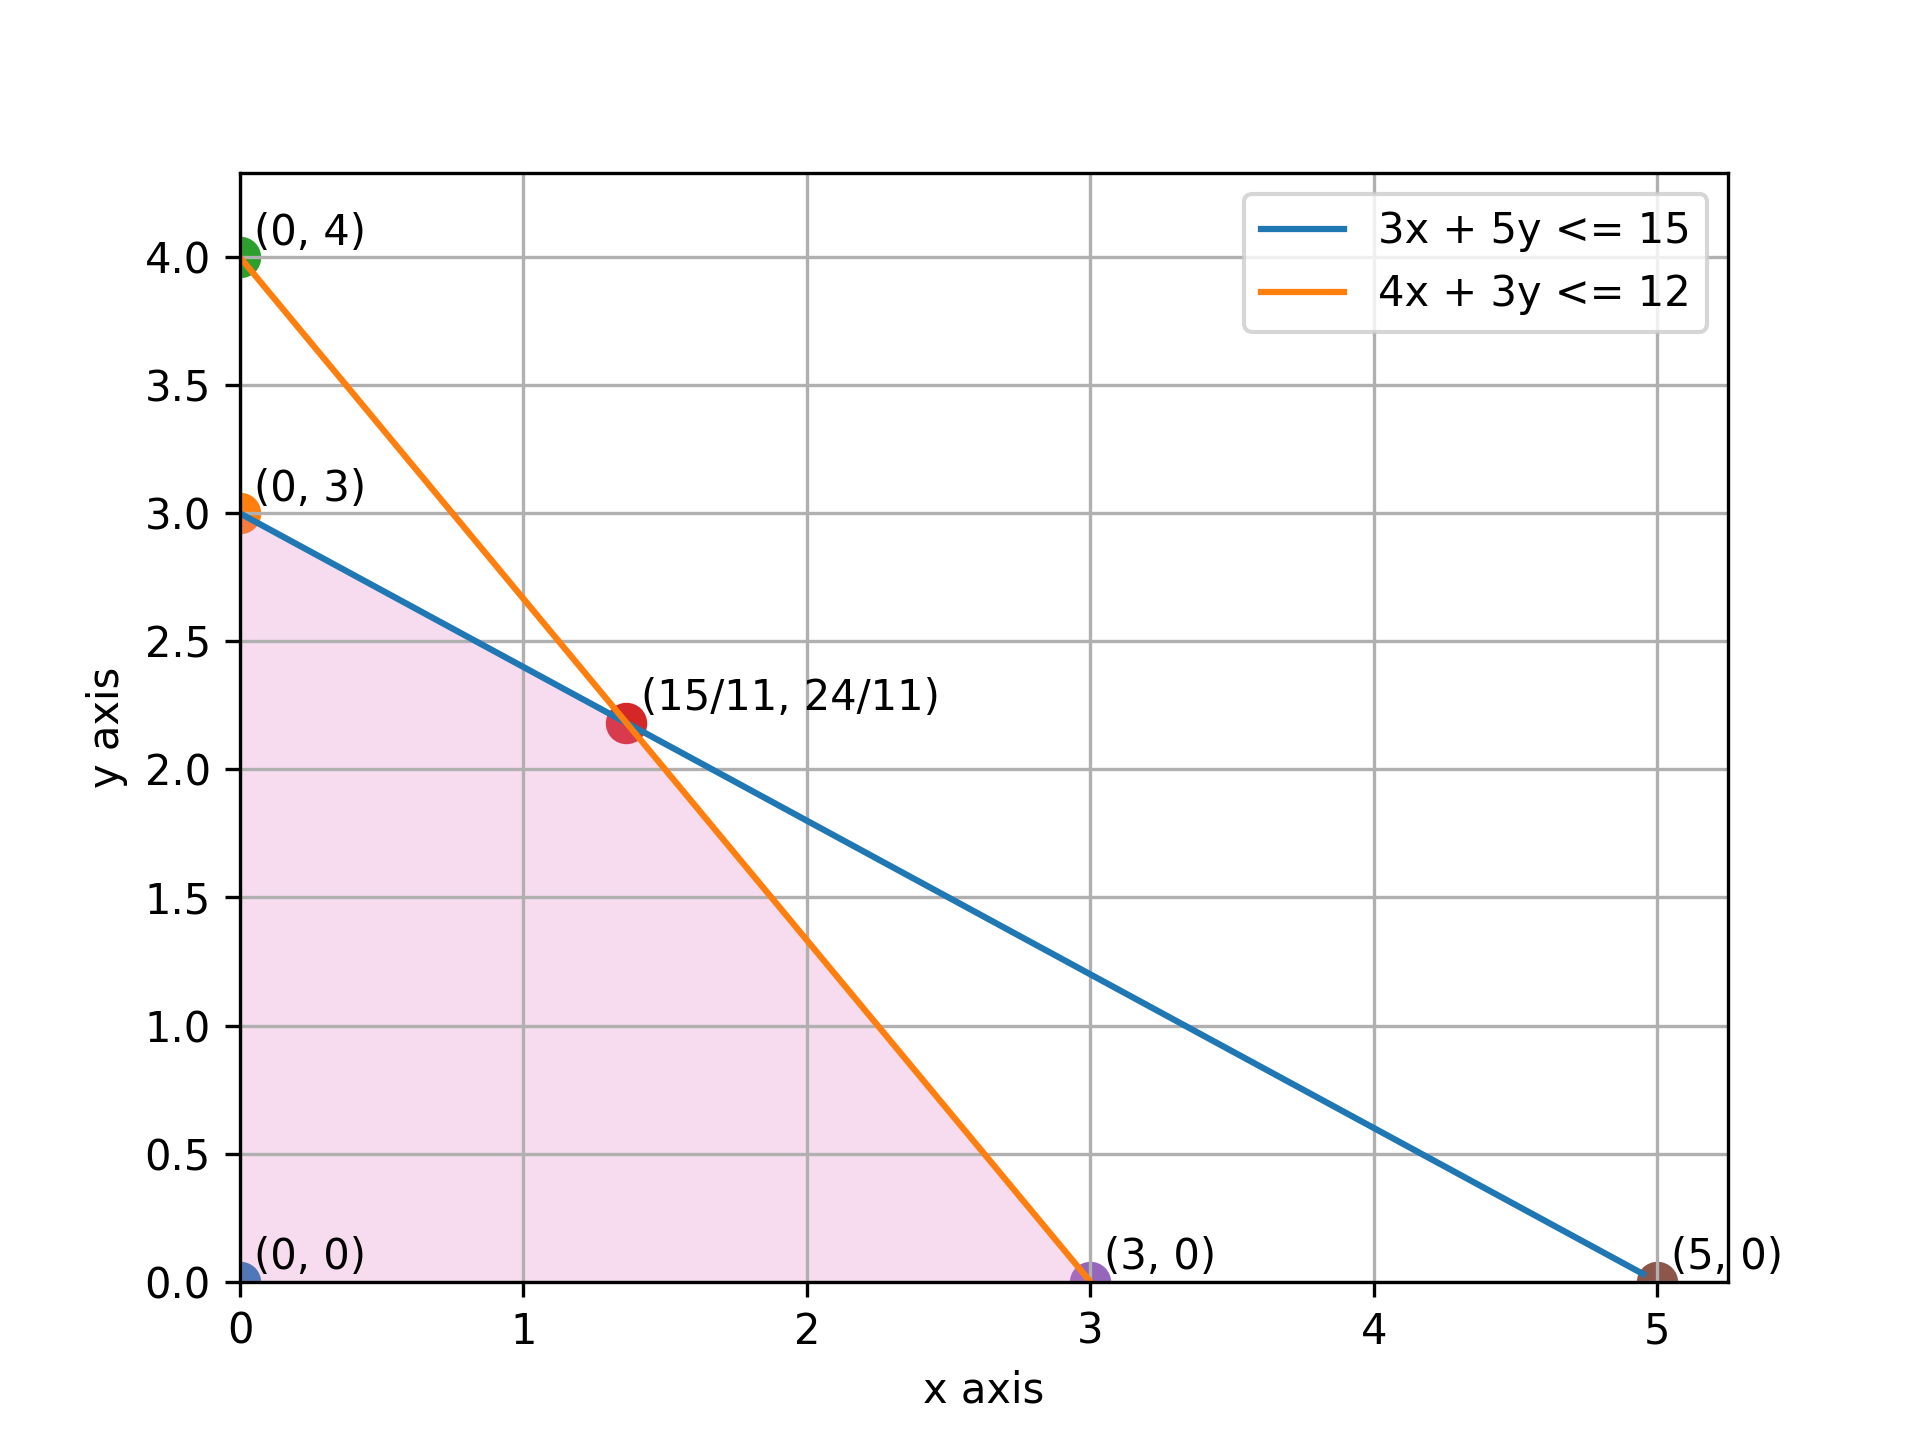
\includegraphics[width=0.6\textwidth]{outputs/graph8.png}
\end{center}
\begin{align*}
Z=15\end{align*}
\begin{align*}
x=3\end{align*}
\begin{align*}
y=0\end{align*}
\begin{align*}
\text{Maximize} \quad & 5x - y\\
\text{subject to} \quad
& 3x + 5y\le15\\
& 4x + 3y\le12\\
& x\ge0,\; y\ge0\end{align*}
Standard Form:\\
\begin{align*}
\text{Maximize} \quad & 5x - y\\
\text{subject to} \quad
& s_{1} + 3x + 5y=15\\
& s_{2} + 4x + 3y=12\\
& x\ge0,\; y\ge0\end{align*}
\begin{align*}
\begin{array}{c|c|c|c|c|c|c|c}
 &  &  & 0 & 0 & 5 & -1 & \\
\hline
\text{BV} & \text{C} & \text{B} & s_{1} & s_{2} & x & y & \text{MR} \\
\hline
s_{1} & 0 & 15 & 1 & 0 & 3 & 5 & 5 \\
s_{2} & 0 & 12 & 0 & 1 & 4 & 3 & 3 \\
\hline
 &  & Z_j-C_j & 0 & 0 & -5 & 1 & \\
\end{array}
\end{align*}
\begin{align*}
\begin{array}{c|c|c|c|c|c|c|c}
 &  &  & 0 & 0 & 5 & -1 & \\
\hline
\text{BV} & \text{C} & \text{B} & s_{1} & s_{2} & x & y & \text{MR} \\
\hline
s_{1} & 0 & 6 & 1 & -\frac{3}{4} & 0 & \frac{11}{4} & 5 \\
x & 5 & 3 & 0 & \frac{1}{4} & 1 & \frac{3}{4} & 3 \\
\hline
 &  & Z_j-C_j & 0 & \frac{5}{4} & 0 & \frac{19}{4} & \\
\end{array}
\end{align*}
\begin{align*}
\left.5x - y\right|_{s_{1}=0,s_{2}=0,x=3,y=0}=15\end{align*}
\begin{align*}
Z=15\end{align*}
\begin{align*}
x=3\end{align*}
\begin{align*}
y=0\end{align*}
\begin{align*}
\text{Maximize} \quad & x_{1} + x_{2}\\
\text{subject to} \quad
& x_{1} + x_{2}\le8\\
& 2x_{1} + x_{2}\le10\\
& x_{1}\ge0,\; x_{2}\ge0\end{align*}
Standard Form:\\
\begin{align*}
\text{Maximize} \quad & x_{1} + x_{2}\\
\text{subject to} \quad
& s_{1} + x_{1} + x_{2}=8\\
& s_{2} + 2x_{1} + x_{2}=10\\
& x_{1}\ge0,\; x_{2}\ge0\end{align*}
\begin{align*}
\begin{array}{c|c|c|c|c|c|c|c}
 &  &  & 0 & 0 & 1 & 1 & \\
\hline
\text{BV} & \text{C} & \text{B} & s_{1} & s_{2} & x_{1} & x_{2} & \text{MR} \\
\hline
s_{1} & 0 & 8 & 1 & 0 & 1 & 1 & 8 \\
s_{2} & 0 & 10 & 0 & 1 & 2 & 1 & 5 \\
\hline
 &  & Z_j-C_j & 0 & 0 & -1 & -1 & \\
\end{array}
\end{align*}
\begin{align*}
\begin{array}{c|c|c|c|c|c|c|c}
 &  &  & 0 & 0 & 1 & 1 & \\
\hline
\text{BV} & \text{C} & \text{B} & s_{1} & s_{2} & x_{1} & x_{2} & \text{MR} \\
\hline
s_{1} & 0 & 3 & 1 & -\frac{1}{2} & 0 & \frac{1}{2} & 6 \\
x_{1} & 1 & 5 & 0 & \frac{1}{2} & 1 & \frac{1}{2} & 10 \\
\hline
 &  & Z_j-C_j & 0 & \frac{1}{2} & 0 & -\frac{1}{2} & \\
\end{array}
\end{align*}
\begin{align*}
5<B_{1}<10\end{align*}
\begin{align*}
8<B_{2}<16\end{align*}
\begin{align*}
\text{Maximize} \quad & -4x - y\\
\text{subject to} \quad
& 3x + y=3\\
& 4x + 3y\ge6\\
& x + 2y\le3\\
& x\ge0,\; y\ge0\end{align*}
Standard Form:\\
\begin{align*}
\text{Maximize} \quad & -4x - y\\
\text{subject to} \quad
& 3x + y=3\\
& -s_{1} + 4x + 3y=6\\
& s_{2} + x + 2y=3\\
& x\ge0,\; y\ge0\end{align*}
\begin{align*}
\begin{array}{c|c|c|c|c|c|c|c|c|c}
 &  &  & -M & -M & 0 & 0 & -4 & -1 & \\
\hline
\text{BV} & \text{C} & \text{B} & A_{1} & A_{2} & s_{1} & s_{2} & x & y & \text{MR} \\
\hline
A_{1} & -M & 3 & 1 & 0 & 0 & 0 & 3 & 1 & 1 \\
A_{2} & -M & 6 & 0 & 1 & -1 & 0 & 4 & 3 & \frac{3}{2} \\
s_{2} & 0 & 3 & 0 & 0 & 0 & 1 & 1 & 2 & 3 \\
\hline
 &  & Z_j-C_j & 0 & 0 & M & 0 & -7M + 4 & -4M + 1 & \\
\end{array}
\end{align*}
\begin{align*}
\begin{array}{c|c|c|c|c|c|c|c|c}
 &  &  & -M & 0 & 0 & -4 & -1 & \\
\hline
\text{BV} & \text{C} & \text{B} & A_{2} & s_{1} & s_{2} & x & y & \text{MR} \\
\hline
x & -4 & 1 & 0 & 0 & 0 & 1 & \frac{1}{3} & 3 \\
A_{2} & -M & 2 & 1 & -1 & 0 & 0 & \frac{5}{3} & \frac{6}{5} \\
s_{2} & 0 & 2 & 0 & 0 & 1 & 0 & \frac{5}{3} & \frac{6}{5} \\
\hline
 &  & Z_j-C_j & 0 & M & 0 & 0 & \dfrac{-5M}{3} - \frac{1}{3} & \\
\end{array}
\end{align*}
\begin{align*}
\begin{array}{c|c|c|c|c|c|c|c}
 &  &  & 0 & 0 & -4 & -1 & \\
\hline
\text{BV} & \text{C} & \text{B} & s_{1} & s_{2} & x & y & \text{MR} \\
\hline
x & -4 & \frac{3}{5} & \frac{1}{5} & 0 & 1 & 0 & 3 \\
y & -1 & \frac{6}{5} & -\frac{3}{5} & 0 & 0 & 1 & - \\
s_{2} & 0 & 0 & 1 & 1 & 0 & 0 & 0 \\
\hline
 &  & Z_j-C_j & -\frac{1}{5} & 0 & 0 & 0 & \\
\end{array}
\end{align*}
\begin{align*}
\begin{array}{c|c|c|c|c|c|c|c}
 &  &  & 0 & 0 & -4 & -1 & \\
\hline
\text{BV} & \text{C} & \text{B} & s_{1} & s_{2} & x & y & \text{MR} \\
\hline
x & -4 & \frac{3}{5} & 0 & -\frac{1}{5} & 1 & 0 & 3 \\
y & -1 & \frac{6}{5} & 0 & \frac{3}{5} & 0 & 1 & - \\
s_{1} & 0 & 0 & 1 & 1 & 0 & 0 & 0 \\
\hline
 &  & Z_j-C_j & 0 & \frac{1}{5} & 0 & 0 & \\
\end{array}
\end{align*}
\begin{align*}
\left.-4x - y\right|_{s_{1}=0,s_{2}=0,x=\frac{3}{5},y=\frac{6}{5}}=-\frac{18}{5}\end{align*}
\begin{align*}
Z=-\frac{18}{5}\end{align*}
\begin{align*}
x=\frac{3}{5}\end{align*}
\begin{align*}
y=\frac{6}{5}\end{align*}
\begin{align*}
\text{Minimize} \quad & x_{1} - 3x_{2} + 2x_{3}\\
\text{subject to} \quad
& 3x_{1} - x_{2} + 2x_{3}\le7\\
& -2x_{1} + 4x_{2}\le12\\
& -4x_{1} + 3x_{2} + 8x_{3}\le10\\
& x_{1}\ge0,\; x_{2}\ge0,\; x_{3}\ge0\end{align*}
Standard Form:\\
\begin{align*}
\text{Maximize} \quad & -x_{1} + 3x_{2} - 2x_{3}\\
\text{subject to} \quad
& s_{1} + 3x_{1} - x_{2} + 2x_{3}=7\\
& s_{2} - 2x_{1} + 4x_{2}=12\\
& s_{3} - 4x_{1} + 3x_{2} + 8x_{3}=10\\
& x_{1}\ge0,\; x_{2}\ge0,\; x_{3}\ge0\end{align*}
\begin{align*}
\begin{array}{c|c|c|c|c|c|c|c|c|c}
 &  &  & 0 & 0 & 0 & -1 & 3 & -2 & \\
\hline
\text{BV} & \text{C} & \text{B} & s_{1} & s_{2} & s_{3} & x_{1} & x_{2} & x_{3} & \text{MR} \\
\hline
s_{1} & 0 & 7 & 1 & 0 & 0 & 3 & -1 & 2 & - \\
s_{2} & 0 & 12 & 0 & 1 & 0 & -2 & 4 & 0 & 3 \\
s_{3} & 0 & 10 & 0 & 0 & 1 & -4 & 3 & 8 & \frac{10}{3} \\
\hline
 &  & Z_j-C_j & 0 & 0 & 0 & 1 & -3 & 2 & \\
\end{array}
\end{align*}
\begin{align*}
\begin{array}{c|c|c|c|c|c|c|c|c|c}
 &  &  & 0 & 0 & 0 & -1 & 3 & -2 & \\
\hline
\text{BV} & \text{C} & \text{B} & s_{1} & s_{2} & s_{3} & x_{1} & x_{2} & x_{3} & \text{MR} \\
\hline
s_{1} & 0 & 10 & 1 & \frac{1}{4} & 0 & \frac{5}{2} & 0 & 2 & 4 \\
x_{2} & 3 & 3 & 0 & \frac{1}{4} & 0 & -\frac{1}{2} & 1 & 0 & - \\
s_{3} & 0 & 1 & 0 & -\frac{3}{4} & 1 & -\frac{5}{2} & 0 & 8 & - \\
\hline
 &  & Z_j-C_j & 0 & \frac{3}{4} & 0 & -\frac{1}{2} & 0 & 2 & \\
\end{array}
\end{align*}
\begin{align*}
\begin{array}{c|c|c|c|c|c|c|c|c|c}
 &  &  & 0 & 0 & 0 & -1 & 3 & -2 & \\
\hline
\text{BV} & \text{C} & \text{B} & s_{1} & s_{2} & s_{3} & x_{1} & x_{2} & x_{3} & \text{MR} \\
\hline
x_{1} & -1 & 4 & \frac{2}{5} & \frac{1}{10} & 0 & 1 & 0 & \frac{4}{5} & 4 \\
x_{2} & 3 & 5 & \frac{1}{5} & \frac{3}{10} & 0 & 0 & 1 & \frac{2}{5} & - \\
s_{3} & 0 & 11 & 1 & -\frac{1}{2} & 1 & 0 & 0 & 10 & - \\
\hline
 &  & Z_j-C_j & \frac{1}{5} & \frac{4}{5} & 0 & 0 & 0 & \frac{12}{5} & \\
\end{array}
\end{align*}
\begin{align*}
\left.-x_{1} + 3x_{2} - 2x_{3}\right|_{s_{1}=0,s_{2}=0,s_{3}=0,x_{1}=4,x_{2}=5,x_{3}=0}=11\end{align*}
\begin{align*}
Z=-11\end{align*}
\begin{align*}
x_{1}=4\end{align*}
\begin{align*}
x_{2}=5\end{align*}
\begin{align*}
x_{3}=0\end{align*}
\begin{align*}
\text{Minimize} \quad & 5x + 6y\\
\text{subject to} \quad
& x + y\ge2\\
& 4x + y\ge4\\
& x\ge0,\; y\ge0\end{align*}
Canonical Form:\\
\begin{align*}
\text{Minimize} \quad & 5x + 6y\\
\text{subject to} \quad
& x + y\ge2\\
& 4x + y\ge4\\
& x\ge0,\; y\ge0\end{align*}
\begin{align*}
\text{Minimize} \quad & 5x + 6y\\
\text{subject to} \quad
& x + y\ge2\\
& 4x + y\ge4\\
& x\ge0,\; y\ge0\end{align*}
Standard Form:\\
\begin{align*}
\text{Maximize} \quad & -5x - 6y\\
\text{subject to} \quad
& s_{1} - x - y=-2\\
& s_{2} - 4x - y=-4\\
& x\ge0,\; y\ge0\end{align*}
\begin{align*}
\begin{array}{c|c|c|c|c|c|c|c}
 &  &  & 0 & 0 & -5 & -6 & \\
\hline
\text{BV} & \text{C} & \text{B} & s_{1} & s_{2} & x & y & \text{MR} \\
\hline
s_{1} & 0 & -2 & 1 & 0 & -1 & -1 \\
s_{2} & 0 & -4 & 0 & 1 & -4 & -1 \\
\hline
 &  & Z_j-C_j & 0 & 0 & 5 & 6 & \\
\end{array}
\end{align*}
\begin{align*}
\left.-5x - 6y\right|_{s_{1}=0,s_{2}=0,x=0,y=0}=0\end{align*}
\begin{align*}
Z=0\end{align*}
\begin{align*}
x=0\end{align*}
\begin{align*}
y=0\end{align*}
\begin{align*}
\text{Maximize} \quad & 3x_{1} + 5x_{2}\\
\text{subject to} \quad
& x_{1} + x_{2}\le1\\
& 2x_{1} + 3x_{2}\le1\\
& x\ge0,\; y\ge0\end{align*}
Standard Form:\\
\begin{align*}
\text{Maximize} \quad & 3x_{1} + 5x_{2}\\
\text{subject to} \quad
& s_{1} + x_{1} + x_{2}=1\\
& s_{2} + 2x_{1} + 3x_{2}=1\\
& x\ge0,\; y\ge0\end{align*}
\begin{align*}
\begin{array}{c|c|c|c|c|c|c|c}
 &  &  & 0 & 0 & 3 & 5 & \\
\hline
\text{BV} & \text{C} & \text{B} & s_{1} & s_{2} & x_{1} & x_{2} & \text{MR} \\
\hline
s_{1} & 0 & 1 & 1 & 0 & 1 & 1 & 1 \\
s_{2} & 0 & 1 & 0 & 1 & 2 & 3 & \frac{1}{3} \\
\hline
 &  & Z_j-C_j & 0 & 0 & -3 & -5 & \\
\end{array}
\end{align*}
\begin{align*}
\infty<C_{x1}<\frac{10}{3}\end{align*}
\begin{align*}
9<C_{x2}<\infty\end{align*}
\begin{align*}
\text{Maximize} \quad & x + 4y\\
\text{subject to} \quad
& 2x + 4y\le7\\
& 5x + 3y\le15\\
& x\ge0,\; y\ge0\end{align*}
\begin{align*}
2x + 4y=7\end{align*}
\begin{align*}
5x + 3y=15\end{align*}
Gauss Elimination:\\
Echelon Form:\\
\begin{align*}
\left(
\begin{array}{cc|c}
2 & 4 & 7\\
5 & 3 & 15\\
\end{array}
\right)_{2\times 3}
\end{align*}
\begin{align*}
\left(
\begin{array}{cc|c}
2 & 4 & 7\\
0 & -7 & -\frac{5}{2}\\
\end{array}
\right)_{2\times 3}
\end{align*}
\begin{align*}
\left(
\begin{array}{cc|c}
2 & 4 & 7\\
0 & -7 & -\frac{5}{2}\\
\end{array}
\right)_{2\times 3}
\end{align*}
\begin{align*}
x=\frac{39}{14}\end{align*}
\begin{align*}
y=\frac{5}{14}\end{align*}
\begin{center}

\includegraphics[width=0.6\textwidth]{outputs/ipp1/graph1.png}
\end{center}
\begin{align*}
Z=7\end{align*}
\begin{align*}
x=0\end{align*}
\begin{align*}
y=7\end{align*}
\begin{align*}
\text{Maximize} \quad & x + 4y\\
\text{subject to} \quad
& 2x + 4y\le7\\
& 5x + 3y\le15\\
& y\le1\\
& x\ge0,\; y\ge0\end{align*}
\begin{align*}
2x + 4y=7\end{align*}
\begin{align*}
5x + 3y=15\end{align*}
Gauss Elimination:\\
Echelon Form:\\
\begin{align*}
\left(
\begin{array}{cc|c}
2 & 4 & 7\\
5 & 3 & 15\\
\end{array}
\right)_{2\times 3}
\end{align*}
\begin{align*}
\left(
\begin{array}{cc|c}
2 & 4 & 7\\
0 & -7 & -\frac{5}{2}\\
\end{array}
\right)_{2\times 3}
\end{align*}
\begin{align*}
\left(
\begin{array}{cc|c}
2 & 4 & 7\\
0 & -7 & -\frac{5}{2}\\
\end{array}
\right)_{2\times 3}
\end{align*}
\begin{align*}
x=\frac{39}{14}\end{align*}
\begin{align*}
y=\frac{5}{14}\end{align*}
\begin{align*}
2x + 4y=7\end{align*}
\begin{align*}
y=1\end{align*}
Gauss Elimination:\\
Echelon Form:\\
\begin{align*}
\left(
\begin{array}{cc|c}
2 & 4 & 7\\
0 & 1 & 1\\
\end{array}
\right)_{2\times 3}
\end{align*}
\begin{align*}
\left(
\begin{array}{cc|c}
2 & 4 & 7\\
0 & 1 & 1\\
\end{array}
\right)_{2\times 3}
\end{align*}
\begin{align*}
\left(
\begin{array}{cc|c}
2 & 4 & 7\\
0 & 1 & 1\\
\end{array}
\right)_{2\times 3}
\end{align*}
\begin{align*}
x=\frac{3}{2}\end{align*}
\begin{align*}
y=1\end{align*}
\begin{align*}
5x + 3y=15\end{align*}
\begin{align*}
y=1\end{align*}
Gauss Elimination:\\
Echelon Form:\\
\begin{align*}
\left(
\begin{array}{cc|c}
5 & 3 & 15\\
0 & 1 & 1\\
\end{array}
\right)_{2\times 3}
\end{align*}
\begin{align*}
\left(
\begin{array}{cc|c}
5 & 3 & 15\\
0 & 1 & 1\\
\end{array}
\right)_{2\times 3}
\end{align*}
\begin{align*}
\left(
\begin{array}{cc|c}
5 & 3 & 15\\
0 & 1 & 1\\
\end{array}
\right)_{2\times 3}
\end{align*}
\begin{align*}
x=\frac{12}{5}\end{align*}
\begin{align*}
y=1\end{align*}
\begin{center}

\includegraphics[width=0.6\textwidth]{outputs/ipp1/graph2.png}
\end{center}
\begin{align*}
Z=11\end{align*}
\begin{align*}
x=3\end{align*}
\begin{align*}
y=1\end{align*}
\begin{align*}
\text{Maximize} \quad & x + 4y\\
\text{subject to} \quad
& 2x + 4y\le7\\
& 5x + 3y\le15\\
& y\ge2\\
& x\ge0,\; y\ge0\end{align*}
\begin{align*}
2x + 4y=7\end{align*}
\begin{align*}
5x + 3y=15\end{align*}
Gauss Elimination:\\
Echelon Form:\\
\begin{align*}
\left(
\begin{array}{cc|c}
2 & 4 & 7\\
5 & 3 & 15\\
\end{array}
\right)_{2\times 3}
\end{align*}
\begin{align*}
\left(
\begin{array}{cc|c}
2 & 4 & 7\\
0 & -7 & -\frac{5}{2}\\
\end{array}
\right)_{2\times 3}
\end{align*}
\begin{align*}
\left(
\begin{array}{cc|c}
2 & 4 & 7\\
0 & -7 & -\frac{5}{2}\\
\end{array}
\right)_{2\times 3}
\end{align*}
\begin{align*}
x=\frac{39}{14}\end{align*}
\begin{align*}
y=\frac{5}{14}\end{align*}
\begin{align*}
2x + 4y=7\end{align*}
\begin{align*}
y=2\end{align*}
Gauss Elimination:\\
Echelon Form:\\
\begin{align*}
\left(
\begin{array}{cc|c}
2 & 4 & 7\\
0 & 1 & 2\\
\end{array}
\right)_{2\times 3}
\end{align*}
\begin{align*}
\left(
\begin{array}{cc|c}
2 & 4 & 7\\
0 & 1 & 2\\
\end{array}
\right)_{2\times 3}
\end{align*}
\begin{align*}
\left(
\begin{array}{cc|c}
2 & 4 & 7\\
0 & 1 & 2\\
\end{array}
\right)_{2\times 3}
\end{align*}
\begin{align*}
x=-\frac{1}{2}\end{align*}
\begin{align*}
y=2\end{align*}
\begin{align*}
5x + 3y=15\end{align*}
\begin{align*}
y=2\end{align*}
Gauss Elimination:\\
Echelon Form:\\
\begin{align*}
\left(
\begin{array}{cc|c}
5 & 3 & 15\\
0 & 1 & 2\\
\end{array}
\right)_{2\times 3}
\end{align*}
\begin{align*}
\left(
\begin{array}{cc|c}
5 & 3 & 15\\
0 & 1 & 2\\
\end{array}
\right)_{2\times 3}
\end{align*}
\begin{align*}
\left(
\begin{array}{cc|c}
5 & 3 & 15\\
0 & 1 & 2\\
\end{array}
\right)_{2\times 3}
\end{align*}
\begin{align*}
x=\frac{9}{5}\end{align*}
\begin{align*}
y=2\end{align*}
\begin{center}
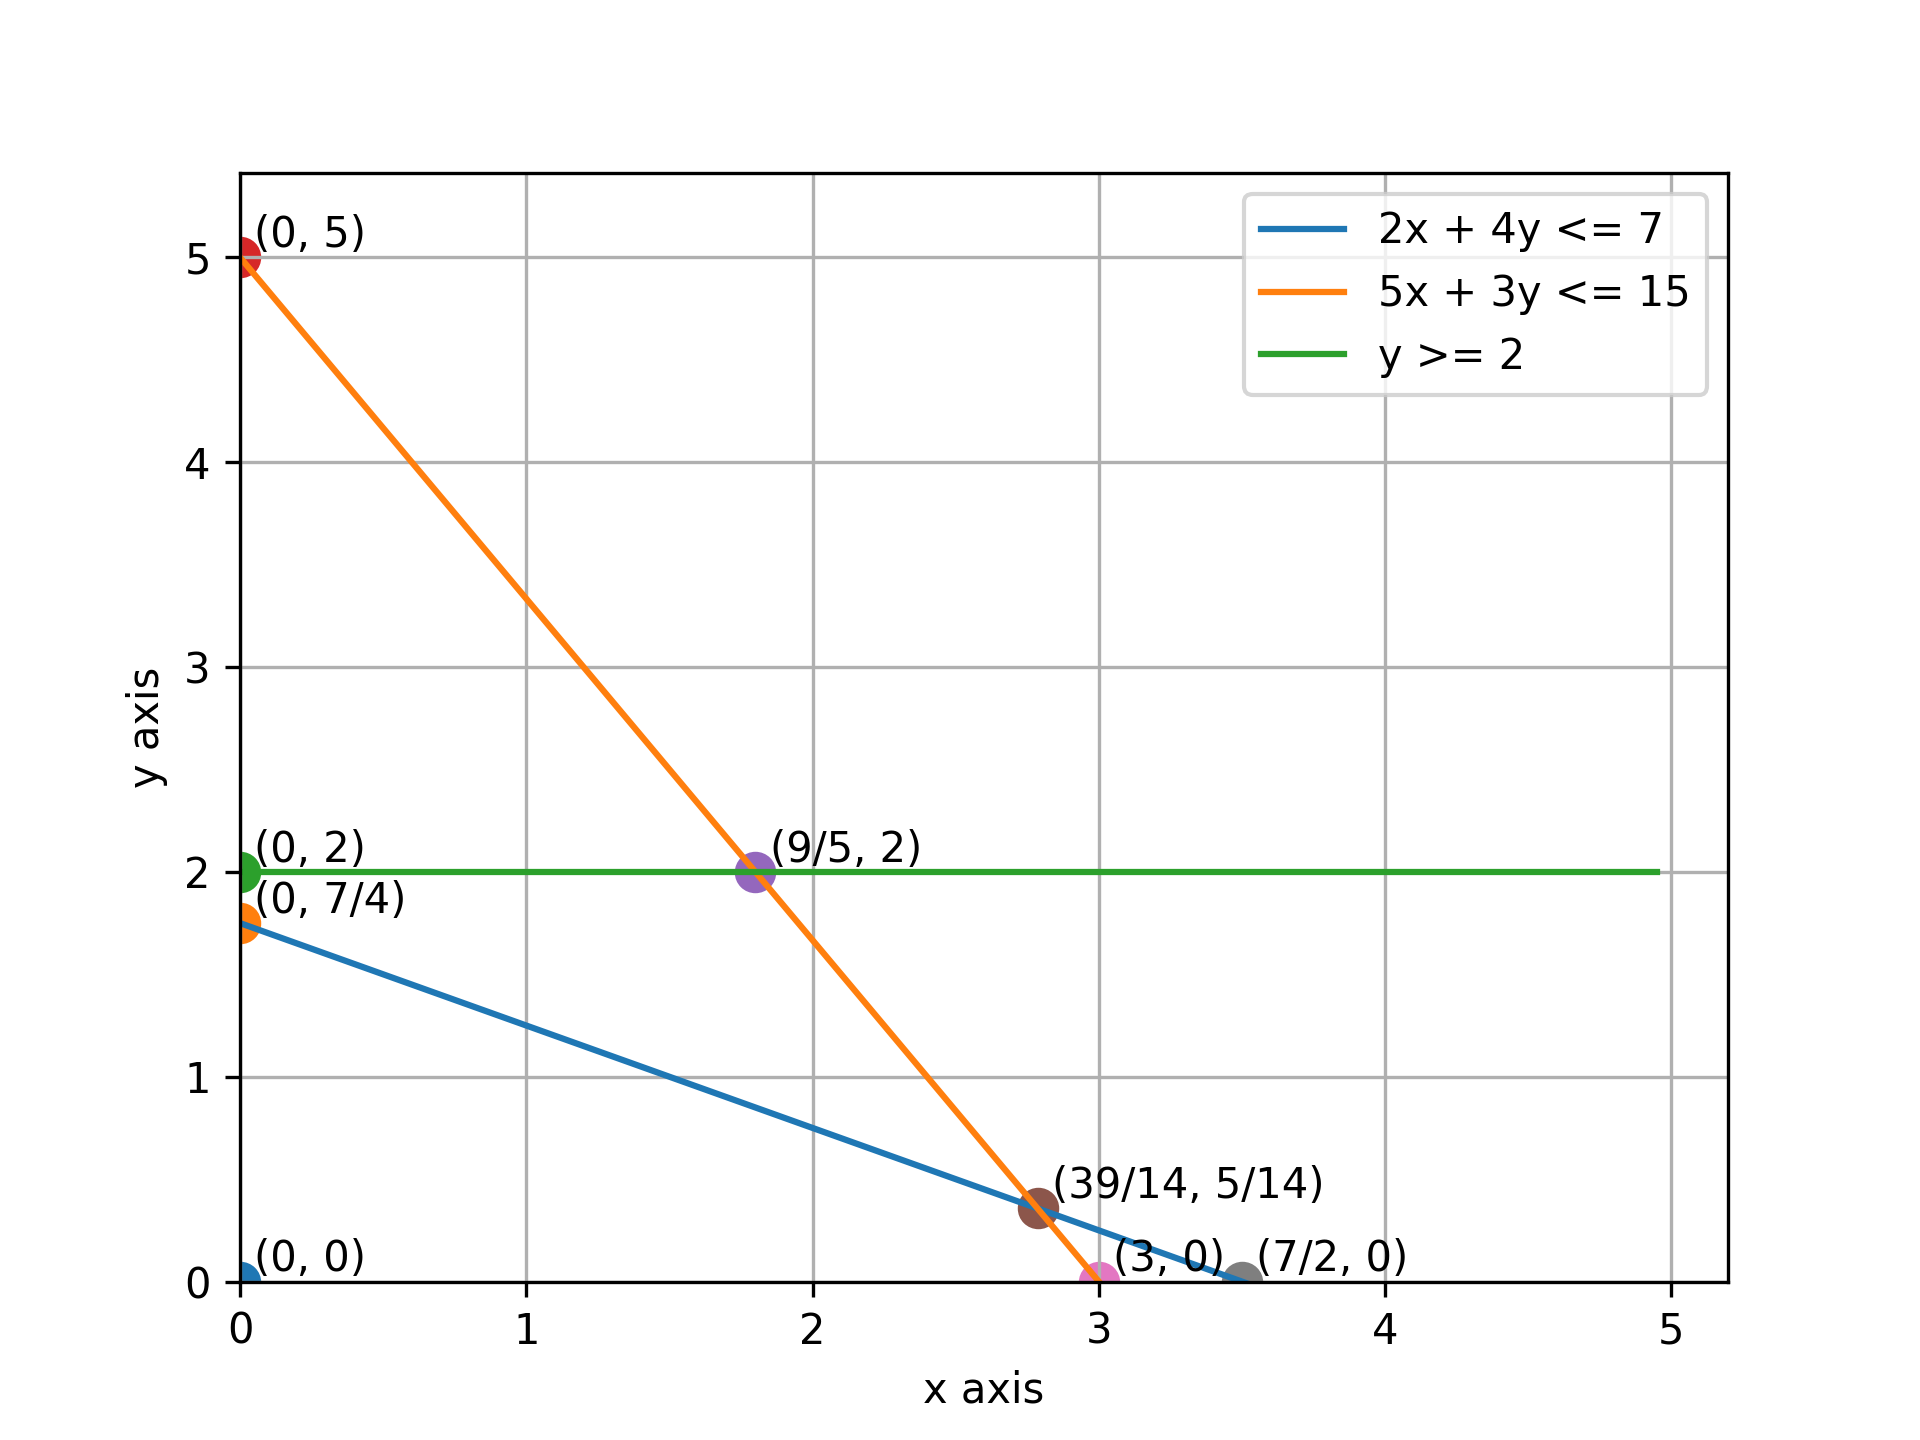
\includegraphics[width=0.6\textwidth]{outputs/ipp1/graph3.png}
\end{center}
Infeasible Solution\\
\begin{align*}
\text{Maximize} \quad & x + 4y\\
\text{subject to} \quad
& 2x + 4y\le7\\
& 5x + 3y\le15\\
& y\le1\\
& x\le1\\
& x\ge0,\; y\ge0\end{align*}
\begin{align*}
2x + 4y=7\end{align*}
\begin{align*}
5x + 3y=15\end{align*}
Gauss Elimination:\\
Echelon Form:\\
\begin{align*}
\left(
\begin{array}{cc|c}
2 & 4 & 7\\
5 & 3 & 15\\
\end{array}
\right)_{2\times 3}
\end{align*}
\begin{align*}
\left(
\begin{array}{cc|c}
2 & 4 & 7\\
0 & -7 & -\frac{5}{2}\\
\end{array}
\right)_{2\times 3}
\end{align*}
\begin{align*}
\left(
\begin{array}{cc|c}
2 & 4 & 7\\
0 & -7 & -\frac{5}{2}\\
\end{array}
\right)_{2\times 3}
\end{align*}
\begin{align*}
x=\frac{39}{14}\end{align*}
\begin{align*}
y=\frac{5}{14}\end{align*}
\begin{align*}
2x + 4y=7\end{align*}
\begin{align*}
y=1\end{align*}
Gauss Elimination:\\
Echelon Form:\\
\begin{align*}
\left(
\begin{array}{cc|c}
2 & 4 & 7\\
0 & 1 & 1\\
\end{array}
\right)_{2\times 3}
\end{align*}
\begin{align*}
\left(
\begin{array}{cc|c}
2 & 4 & 7\\
0 & 1 & 1\\
\end{array}
\right)_{2\times 3}
\end{align*}
\begin{align*}
\left(
\begin{array}{cc|c}
2 & 4 & 7\\
0 & 1 & 1\\
\end{array}
\right)_{2\times 3}
\end{align*}
\begin{align*}
x=\frac{3}{2}\end{align*}
\begin{align*}
y=1\end{align*}
\begin{align*}
2x + 4y=7\end{align*}
\begin{align*}
x=1\end{align*}
Gauss Elimination:\\
Echelon Form:\\
\begin{align*}
\left(
\begin{array}{cc|c}
2 & 4 & 7\\
1 & 0 & 1\\
\end{array}
\right)_{2\times 3}
\end{align*}
\begin{align*}
\left(
\begin{array}{cc|c}
2 & 4 & 7\\
0 & -2 & -\frac{5}{2}\\
\end{array}
\right)_{2\times 3}
\end{align*}
\begin{align*}
\left(
\begin{array}{cc|c}
2 & 4 & 7\\
0 & -2 & -\frac{5}{2}\\
\end{array}
\right)_{2\times 3}
\end{align*}
\begin{align*}
x=1\end{align*}
\begin{align*}
y=\frac{5}{4}\end{align*}
\begin{align*}
5x + 3y=15\end{align*}
\begin{align*}
y=1\end{align*}
Gauss Elimination:\\
Echelon Form:\\
\begin{align*}
\left(
\begin{array}{cc|c}
5 & 3 & 15\\
0 & 1 & 1\\
\end{array}
\right)_{2\times 3}
\end{align*}
\begin{align*}
\left(
\begin{array}{cc|c}
5 & 3 & 15\\
0 & 1 & 1\\
\end{array}
\right)_{2\times 3}
\end{align*}
\begin{align*}
\left(
\begin{array}{cc|c}
5 & 3 & 15\\
0 & 1 & 1\\
\end{array}
\right)_{2\times 3}
\end{align*}
\begin{align*}
x=\frac{12}{5}\end{align*}
\begin{align*}
y=1\end{align*}
\begin{align*}
5x + 3y=15\end{align*}
\begin{align*}
x=1\end{align*}
Gauss Elimination:\\
Echelon Form:\\
\begin{align*}
\left(
\begin{array}{cc|c}
5 & 3 & 15\\
1 & 0 & 1\\
\end{array}
\right)_{2\times 3}
\end{align*}
\begin{align*}
\left(
\begin{array}{cc|c}
5 & 3 & 15\\
0 & -\frac{3}{5} & -2\\
\end{array}
\right)_{2\times 3}
\end{align*}
\begin{align*}
\left(
\begin{array}{cc|c}
5 & 3 & 15\\
0 & -\frac{3}{5} & -2\\
\end{array}
\right)_{2\times 3}
\end{align*}
\begin{align*}
x=1\end{align*}
\begin{align*}
y=\frac{10}{3}\end{align*}
\begin{align*}
y=1\end{align*}
\begin{align*}
x=1\end{align*}
Gauss Elimination:\\
Echelon Form:\\
\begin{align*}
\left(
\begin{array}{cc|c}
0 & 1 & 1\\
1 & 0 & 1\\
\end{array}
\right)_{2\times 3}
\end{align*}
\begin{align*}
\left(
\begin{array}{cc|c}
1 & 0 & 1\\
0 & 1 & 1\\
\end{array}
\right)_{2\times 3}
\end{align*}
\begin{align*}
\left(
\begin{array}{cc|c}
1 & 0 & 1\\
0 & 1 & 1\\
\end{array}
\right)_{2\times 3}
\end{align*}
\begin{align*}
x=1\end{align*}
\begin{align*}
y=1\end{align*}
\begin{center}
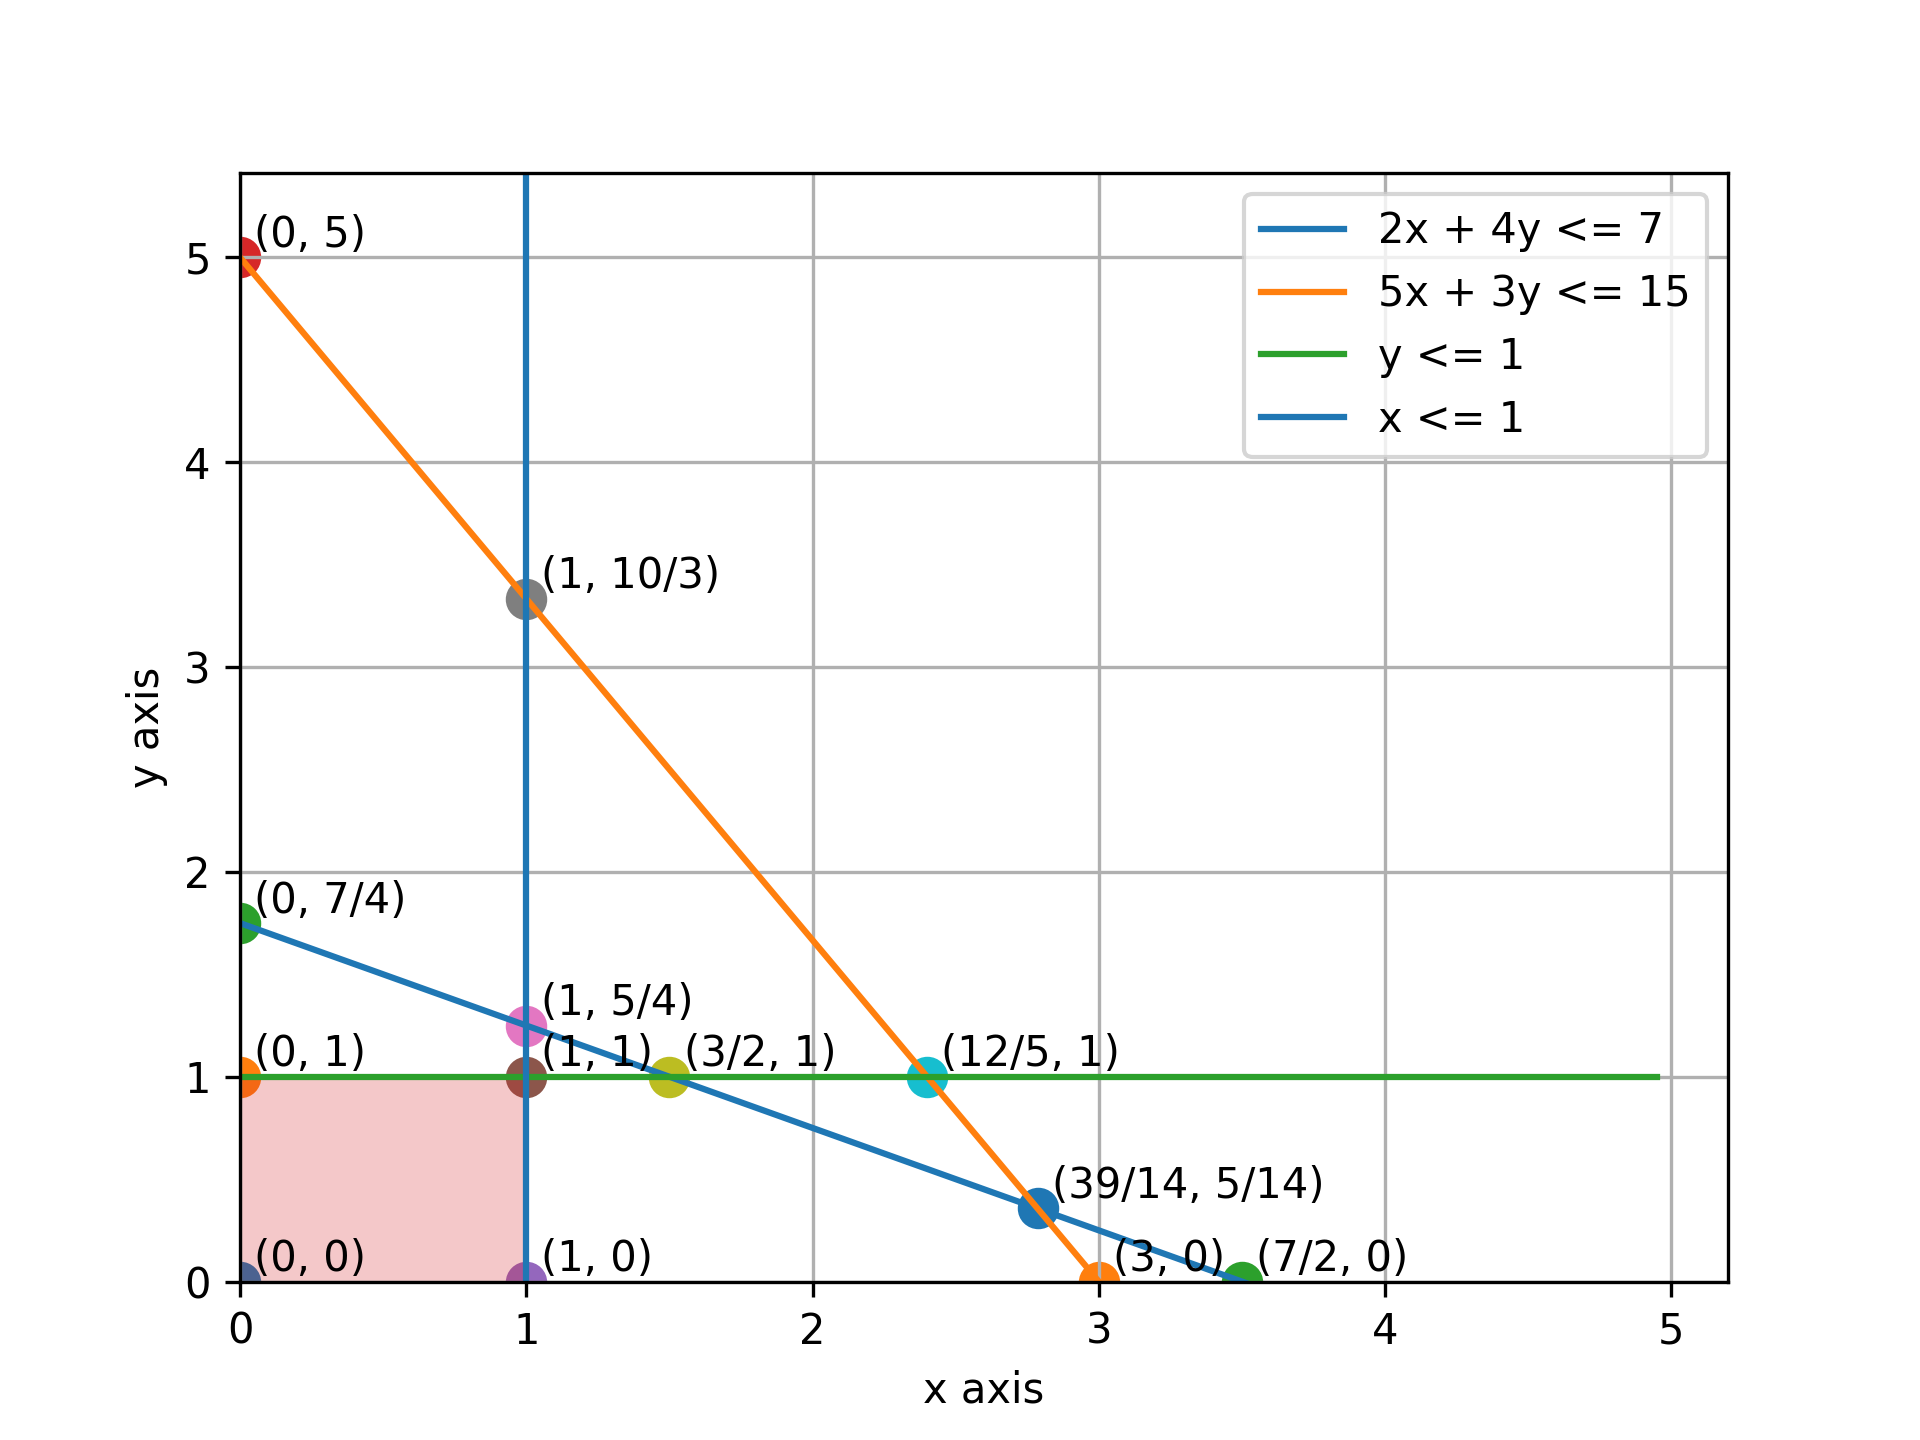
\includegraphics[width=0.6\textwidth]{outputs/ipp1/graph4.png}
\end{center}
\begin{align*}
Z=5\end{align*}
\begin{align*}
x=1\end{align*}
\begin{align*}
y=1\end{align*}
\begin{align*}
\text{Maximize} \quad & x + 4y\\
\text{subject to} \quad
& 2x + 4y\le7\\
& 5x + 3y\le15\\
& y\le1\\
& x\ge2\\
& x\ge0,\; y\ge0\end{align*}
\begin{align*}
2x + 4y=7\end{align*}
\begin{align*}
5x + 3y=15\end{align*}
Gauss Elimination:\\
Echelon Form:\\
\begin{align*}
\left(
\begin{array}{cc|c}
2 & 4 & 7\\
5 & 3 & 15\\
\end{array}
\right)_{2\times 3}
\end{align*}
\begin{align*}
\left(
\begin{array}{cc|c}
2 & 4 & 7\\
0 & -7 & -\frac{5}{2}\\
\end{array}
\right)_{2\times 3}
\end{align*}
\begin{align*}
\left(
\begin{array}{cc|c}
2 & 4 & 7\\
0 & -7 & -\frac{5}{2}\\
\end{array}
\right)_{2\times 3}
\end{align*}
\begin{align*}
x=\frac{39}{14}\end{align*}
\begin{align*}
y=\frac{5}{14}\end{align*}
\begin{align*}
2x + 4y=7\end{align*}
\begin{align*}
y=1\end{align*}
Gauss Elimination:\\
Echelon Form:\\
\begin{align*}
\left(
\begin{array}{cc|c}
2 & 4 & 7\\
0 & 1 & 1\\
\end{array}
\right)_{2\times 3}
\end{align*}
\begin{align*}
\left(
\begin{array}{cc|c}
2 & 4 & 7\\
0 & 1 & 1\\
\end{array}
\right)_{2\times 3}
\end{align*}
\begin{align*}
\left(
\begin{array}{cc|c}
2 & 4 & 7\\
0 & 1 & 1\\
\end{array}
\right)_{2\times 3}
\end{align*}
\begin{align*}
x=\frac{3}{2}\end{align*}
\begin{align*}
y=1\end{align*}
\begin{align*}
2x + 4y=7\end{align*}
\begin{align*}
x=2\end{align*}
Gauss Elimination:\\
Echelon Form:\\
\begin{align*}
\left(
\begin{array}{cc|c}
2 & 4 & 7\\
1 & 0 & 2\\
\end{array}
\right)_{2\times 3}
\end{align*}
\begin{align*}
\left(
\begin{array}{cc|c}
2 & 4 & 7\\
0 & -2 & -\frac{3}{2}\\
\end{array}
\right)_{2\times 3}
\end{align*}
\begin{align*}
\left(
\begin{array}{cc|c}
2 & 4 & 7\\
0 & -2 & -\frac{3}{2}\\
\end{array}
\right)_{2\times 3}
\end{align*}
\begin{align*}
x=2\end{align*}
\begin{align*}
y=\frac{3}{4}\end{align*}
\begin{align*}
5x + 3y=15\end{align*}
\begin{align*}
y=1\end{align*}
Gauss Elimination:\\
Echelon Form:\\
\begin{align*}
\left(
\begin{array}{cc|c}
5 & 3 & 15\\
0 & 1 & 1\\
\end{array}
\right)_{2\times 3}
\end{align*}
\begin{align*}
\left(
\begin{array}{cc|c}
5 & 3 & 15\\
0 & 1 & 1\\
\end{array}
\right)_{2\times 3}
\end{align*}
\begin{align*}
\left(
\begin{array}{cc|c}
5 & 3 & 15\\
0 & 1 & 1\\
\end{array}
\right)_{2\times 3}
\end{align*}
\begin{align*}
x=\frac{12}{5}\end{align*}
\begin{align*}
y=1\end{align*}
\begin{align*}
5x + 3y=15\end{align*}
\begin{align*}
x=2\end{align*}
Gauss Elimination:\\
Echelon Form:\\
\begin{align*}
\left(
\begin{array}{cc|c}
5 & 3 & 15\\
1 & 0 & 2\\
\end{array}
\right)_{2\times 3}
\end{align*}
\begin{align*}
\left(
\begin{array}{cc|c}
5 & 3 & 15\\
0 & -\frac{3}{5} & -1\\
\end{array}
\right)_{2\times 3}
\end{align*}
\begin{align*}
\left(
\begin{array}{cc|c}
5 & 3 & 15\\
0 & -\frac{3}{5} & -1\\
\end{array}
\right)_{2\times 3}
\end{align*}
\begin{align*}
x=2\end{align*}
\begin{align*}
y=\frac{5}{3}\end{align*}
\begin{align*}
y=1\end{align*}
\begin{align*}
x=2\end{align*}
Gauss Elimination:\\
Echelon Form:\\
\begin{align*}
\left(
\begin{array}{cc|c}
0 & 1 & 1\\
1 & 0 & 2\\
\end{array}
\right)_{2\times 3}
\end{align*}
\begin{align*}
\left(
\begin{array}{cc|c}
1 & 0 & 2\\
0 & 1 & 1\\
\end{array}
\right)_{2\times 3}
\end{align*}
\begin{align*}
\left(
\begin{array}{cc|c}
1 & 0 & 2\\
0 & 1 & 1\\
\end{array}
\right)_{2\times 3}
\end{align*}
\begin{align*}
x=2\end{align*}
\begin{align*}
y=1\end{align*}
\begin{center}
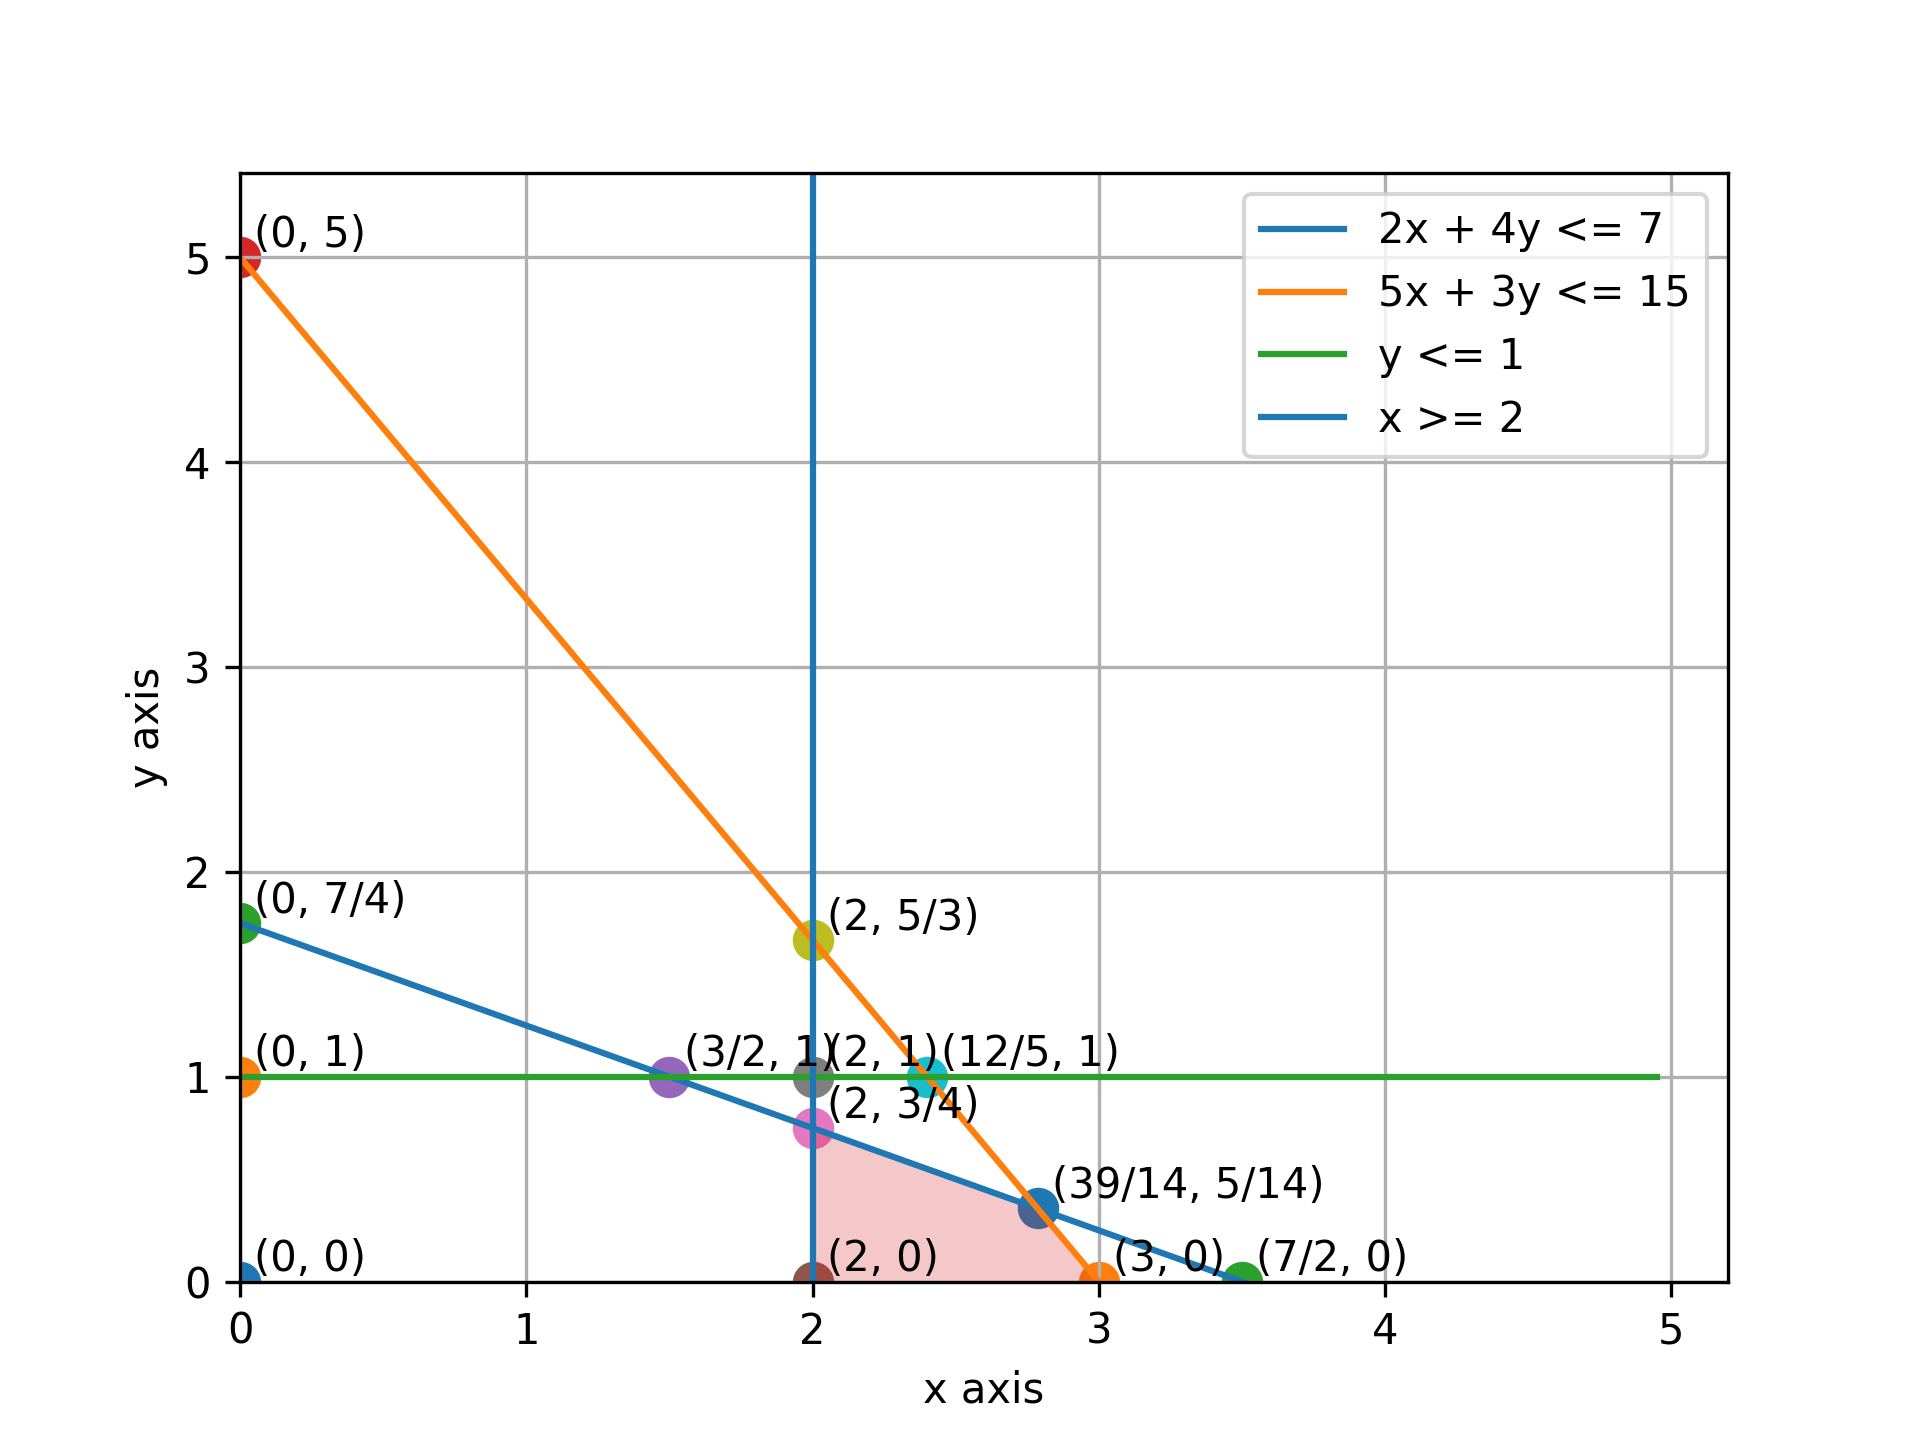
\includegraphics[width=0.6\textwidth]{outputs/ipp1/graph5.png}
\end{center}
\begin{align*}
Z=5\end{align*}
\begin{align*}
x=2\end{align*}
\begin{align*}
y=3\end{align*}
\begin{align*}
\text{Maximize} \quad & x + 4y\\
\text{subject to} \quad
& 2x + 4y\le7\\
& 5x + 3y\le15\\
& y\le1\\
& x\ge2\\
& y\le0\\
& x\ge0,\; y\ge0\end{align*}
\begin{align*}
2x + 4y=7\end{align*}
\begin{align*}
5x + 3y=15\end{align*}
Gauss Elimination:\\
Echelon Form:\\
\begin{align*}
\left(
\begin{array}{cc|c}
2 & 4 & 7\\
5 & 3 & 15\\
\end{array}
\right)_{2\times 3}
\end{align*}
\begin{align*}
\left(
\begin{array}{cc|c}
2 & 4 & 7\\
0 & -7 & -\frac{5}{2}\\
\end{array}
\right)_{2\times 3}
\end{align*}
\begin{align*}
\left(
\begin{array}{cc|c}
2 & 4 & 7\\
0 & -7 & -\frac{5}{2}\\
\end{array}
\right)_{2\times 3}
\end{align*}
\begin{align*}
x=\frac{39}{14}\end{align*}
\begin{align*}
y=\frac{5}{14}\end{align*}
\begin{align*}
2x + 4y=7\end{align*}
\begin{align*}
y=1\end{align*}
Gauss Elimination:\\
Echelon Form:\\
\begin{align*}
\left(
\begin{array}{cc|c}
2 & 4 & 7\\
0 & 1 & 1\\
\end{array}
\right)_{2\times 3}
\end{align*}
\begin{align*}
\left(
\begin{array}{cc|c}
2 & 4 & 7\\
0 & 1 & 1\\
\end{array}
\right)_{2\times 3}
\end{align*}
\begin{align*}
\left(
\begin{array}{cc|c}
2 & 4 & 7\\
0 & 1 & 1\\
\end{array}
\right)_{2\times 3}
\end{align*}
\begin{align*}
x=\frac{3}{2}\end{align*}
\begin{align*}
y=1\end{align*}
\begin{align*}
2x + 4y=7\end{align*}
\begin{align*}
x=2\end{align*}
Gauss Elimination:\\
Echelon Form:\\
\begin{align*}
\left(
\begin{array}{cc|c}
2 & 4 & 7\\
1 & 0 & 2\\
\end{array}
\right)_{2\times 3}
\end{align*}
\begin{align*}
\left(
\begin{array}{cc|c}
2 & 4 & 7\\
0 & -2 & -\frac{3}{2}\\
\end{array}
\right)_{2\times 3}
\end{align*}
\begin{align*}
\left(
\begin{array}{cc|c}
2 & 4 & 7\\
0 & -2 & -\frac{3}{2}\\
\end{array}
\right)_{2\times 3}
\end{align*}
\begin{align*}
x=2\end{align*}
\begin{align*}
y=\frac{3}{4}\end{align*}
\begin{align*}
2x + 4y=7\end{align*}
\begin{align*}
y=0\end{align*}
Gauss Elimination:\\
Echelon Form:\\
\begin{align*}
\left(
\begin{array}{cc|c}
2 & 4 & 7\\
0 & 1 & 0\\
\end{array}
\right)_{2\times 3}
\end{align*}
\begin{align*}
\left(
\begin{array}{cc|c}
2 & 4 & 7\\
0 & 1 & 0\\
\end{array}
\right)_{2\times 3}
\end{align*}
\begin{align*}
\left(
\begin{array}{cc|c}
2 & 4 & 7\\
0 & 1 & 0\\
\end{array}
\right)_{2\times 3}
\end{align*}
\begin{align*}
x=\frac{7}{2}\end{align*}
\begin{align*}
y=0\end{align*}
\begin{align*}
5x + 3y=15\end{align*}
\begin{align*}
y=1\end{align*}
Gauss Elimination:\\
Echelon Form:\\
\begin{align*}
\left(
\begin{array}{cc|c}
5 & 3 & 15\\
0 & 1 & 1\\
\end{array}
\right)_{2\times 3}
\end{align*}
\begin{align*}
\left(
\begin{array}{cc|c}
5 & 3 & 15\\
0 & 1 & 1\\
\end{array}
\right)_{2\times 3}
\end{align*}
\begin{align*}
\left(
\begin{array}{cc|c}
5 & 3 & 15\\
0 & 1 & 1\\
\end{array}
\right)_{2\times 3}
\end{align*}
\begin{align*}
x=\frac{12}{5}\end{align*}
\begin{align*}
y=1\end{align*}
\begin{align*}
5x + 3y=15\end{align*}
\begin{align*}
x=2\end{align*}
Gauss Elimination:\\
Echelon Form:\\
\begin{align*}
\left(
\begin{array}{cc|c}
5 & 3 & 15\\
1 & 0 & 2\\
\end{array}
\right)_{2\times 3}
\end{align*}
\begin{align*}
\left(
\begin{array}{cc|c}
5 & 3 & 15\\
0 & -\frac{3}{5} & -1\\
\end{array}
\right)_{2\times 3}
\end{align*}
\begin{align*}
\left(
\begin{array}{cc|c}
5 & 3 & 15\\
0 & -\frac{3}{5} & -1\\
\end{array}
\right)_{2\times 3}
\end{align*}
\begin{align*}
x=2\end{align*}
\begin{align*}
y=\frac{5}{3}\end{align*}
\begin{align*}
5x + 3y=15\end{align*}
\begin{align*}
y=0\end{align*}
Gauss Elimination:\\
Echelon Form:\\
\begin{align*}
\left(
\begin{array}{cc|c}
5 & 3 & 15\\
0 & 1 & 0\\
\end{array}
\right)_{2\times 3}
\end{align*}
\begin{align*}
\left(
\begin{array}{cc|c}
5 & 3 & 15\\
0 & 1 & 0\\
\end{array}
\right)_{2\times 3}
\end{align*}
\begin{align*}
\left(
\begin{array}{cc|c}
5 & 3 & 15\\
0 & 1 & 0\\
\end{array}
\right)_{2\times 3}
\end{align*}
\begin{align*}
x=3\end{align*}
\begin{align*}
y=0\end{align*}
\begin{align*}
y=1\end{align*}
\begin{align*}
x=2\end{align*}
Gauss Elimination:\\
Echelon Form:\\
\begin{align*}
\left(
\begin{array}{cc|c}
0 & 1 & 1\\
1 & 0 & 2\\
\end{array}
\right)_{2\times 3}
\end{align*}
\begin{align*}
\left(
\begin{array}{cc|c}
1 & 0 & 2\\
0 & 1 & 1\\
\end{array}
\right)_{2\times 3}
\end{align*}
\begin{align*}
\left(
\begin{array}{cc|c}
1 & 0 & 2\\
0 & 1 & 1\\
\end{array}
\right)_{2\times 3}
\end{align*}
\begin{align*}
x=2\end{align*}
\begin{align*}
y=1\end{align*}
\begin{align*}
y=1\end{align*}
\begin{align*}
y=0\end{align*}
Gauss Elimination:\\
Echelon Form:\\
\begin{align*}
\left(
\begin{array}{c|c}
1 & 1\\
1 & 0\\
\end{array}
\right)_{2\times 2}
\end{align*}
\begin{align*}
\left(
\begin{array}{c|c}
1 & 1\\
0 & -1\\
\end{array}
\right)_{2\times 2}
\end{align*}
\begin{align*}
\left(
\begin{array}{c|c}
1 & 1\\
0 & -1\\
\end{array}
\right)_{2\times 2}
\end{align*}
No solution\\
\begin{align*}
x=2\end{align*}
\begin{align*}
y=0\end{align*}
Gauss Elimination:\\
Echelon Form:\\
\begin{align*}
\left(
\begin{array}{cc|c}
1 & 0 & 2\\
0 & 1 & 0\\
\end{array}
\right)_{2\times 3}
\end{align*}
\begin{align*}
\left(
\begin{array}{cc|c}
1 & 0 & 2\\
0 & 1 & 0\\
\end{array}
\right)_{2\times 3}
\end{align*}
\begin{align*}
\left(
\begin{array}{cc|c}
1 & 0 & 2\\
0 & 1 & 0\\
\end{array}
\right)_{2\times 3}
\end{align*}
\begin{align*}
x=2\end{align*}
\begin{align*}
y=0\end{align*}
\begin{center}
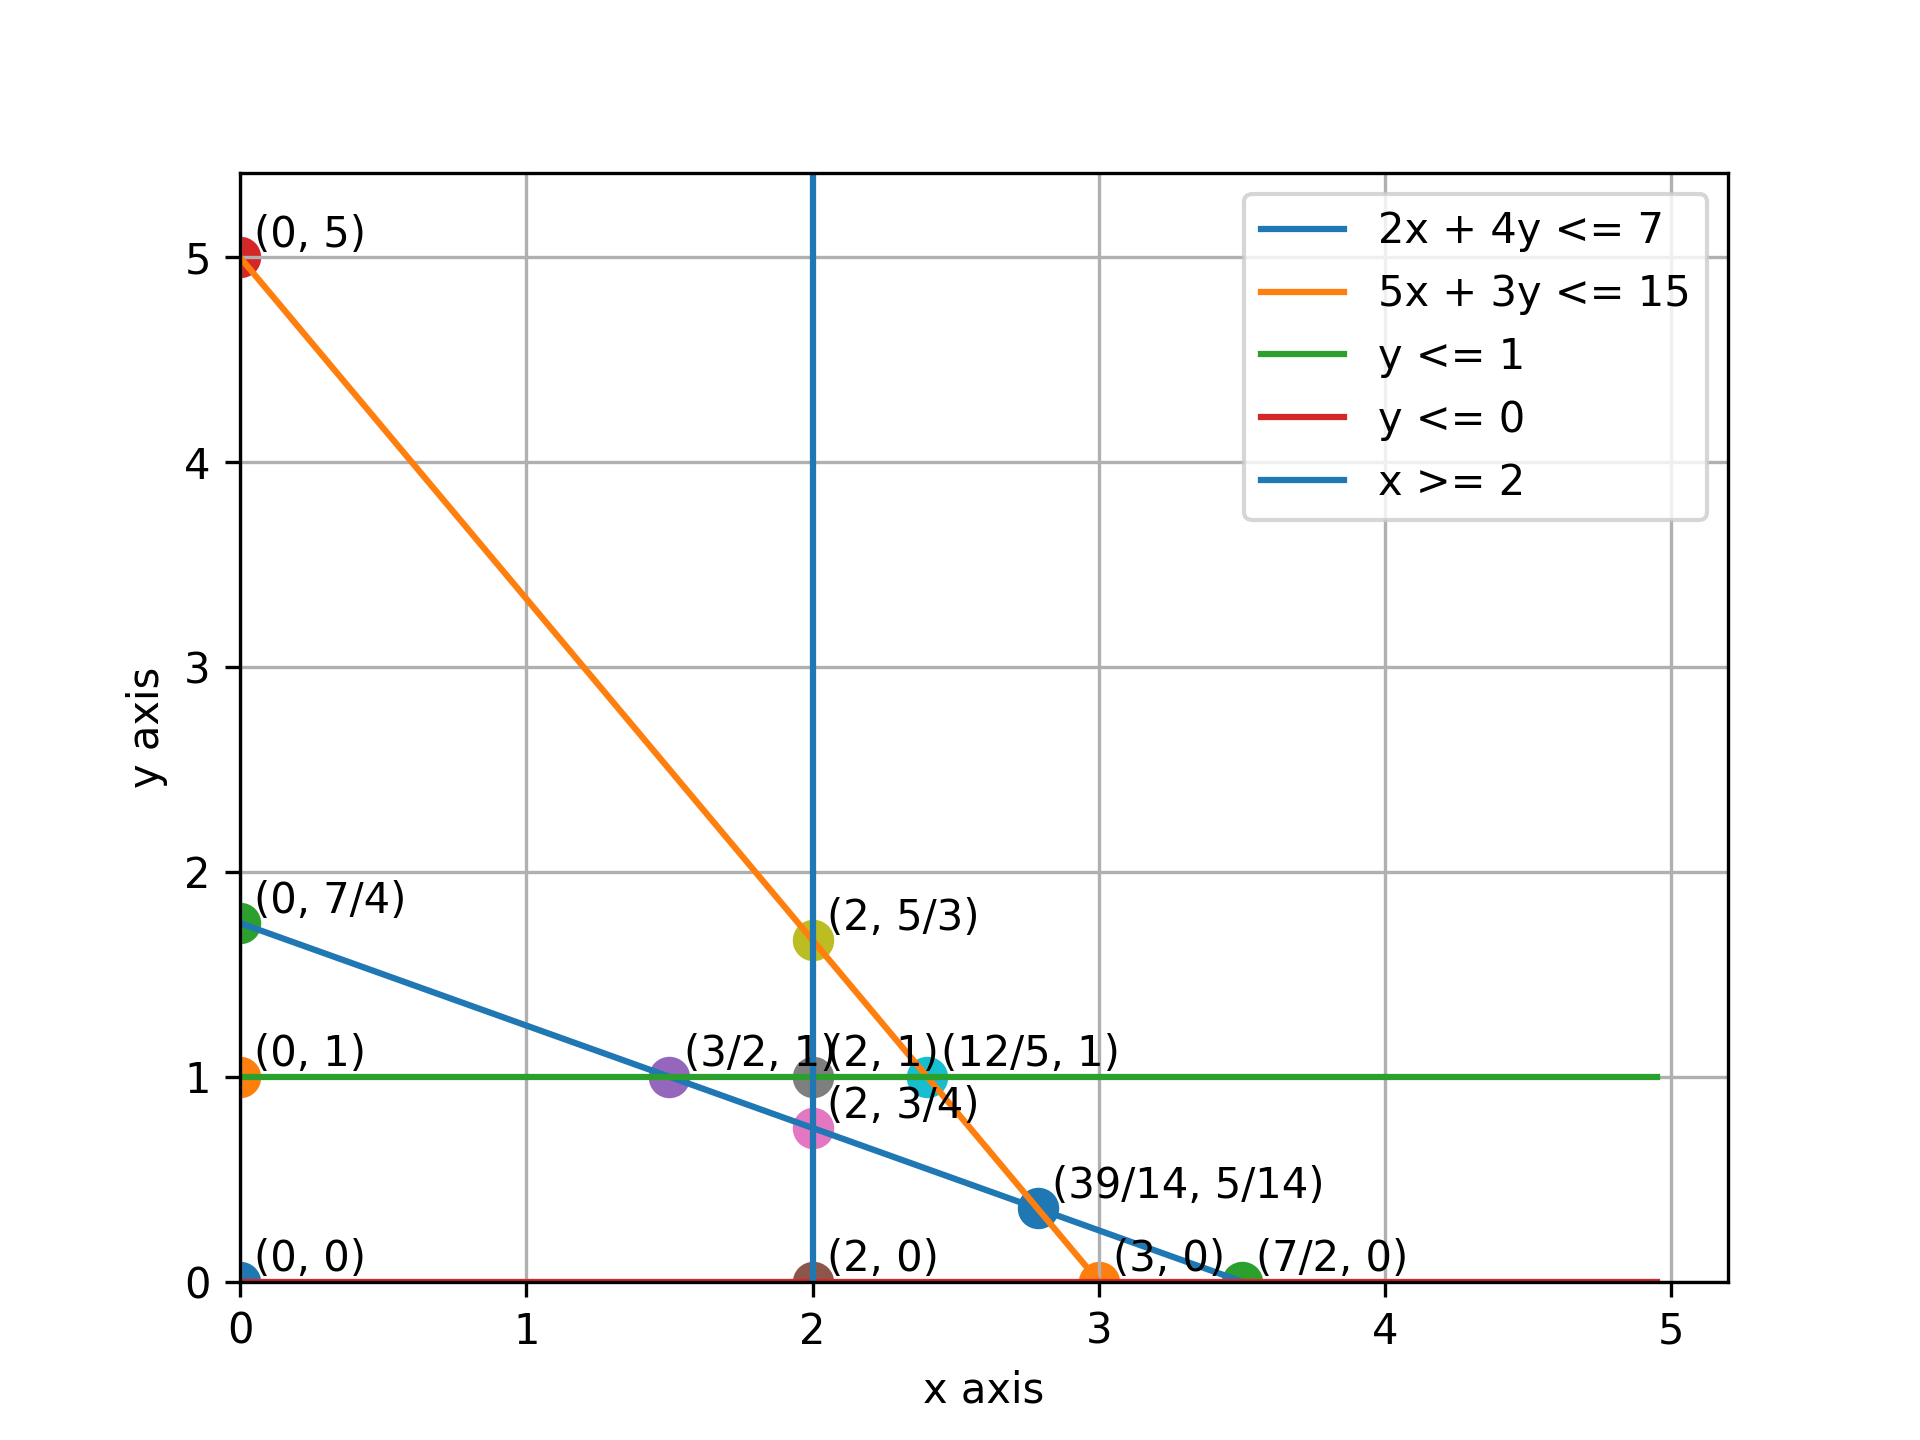
\includegraphics[width=0.6\textwidth]{outputs/ipp1/graph6.png}
\end{center}
\begin{align*}
Z=3\end{align*}
\begin{align*}
x=3\end{align*}
\begin{align*}
y=0\end{align*}
\begin{align*}
\text{Maximize} \quad & x + 4y\\
\text{subject to} \quad
& 2x + 4y\le7\\
& 5x + 3y\le15\\
& y\le1\\
& x\ge2\\
& y\ge1\\
& x\ge0,\; y\ge0\end{align*}
\begin{align*}
2x + 4y=7\end{align*}
\begin{align*}
5x + 3y=15\end{align*}
Gauss Elimination:\\
Echelon Form:\\
\begin{align*}
\left(
\begin{array}{cc|c}
2 & 4 & 7\\
5 & 3 & 15\\
\end{array}
\right)_{2\times 3}
\end{align*}
\begin{align*}
\left(
\begin{array}{cc|c}
2 & 4 & 7\\
0 & -7 & -\frac{5}{2}\\
\end{array}
\right)_{2\times 3}
\end{align*}
\begin{align*}
\left(
\begin{array}{cc|c}
2 & 4 & 7\\
0 & -7 & -\frac{5}{2}\\
\end{array}
\right)_{2\times 3}
\end{align*}
\begin{align*}
x=\frac{39}{14}\end{align*}
\begin{align*}
y=\frac{5}{14}\end{align*}
\begin{align*}
2x + 4y=7\end{align*}
\begin{align*}
y=1\end{align*}
Gauss Elimination:\\
Echelon Form:\\
\begin{align*}
\left(
\begin{array}{cc|c}
2 & 4 & 7\\
0 & 1 & 1\\
\end{array}
\right)_{2\times 3}
\end{align*}
\begin{align*}
\left(
\begin{array}{cc|c}
2 & 4 & 7\\
0 & 1 & 1\\
\end{array}
\right)_{2\times 3}
\end{align*}
\begin{align*}
\left(
\begin{array}{cc|c}
2 & 4 & 7\\
0 & 1 & 1\\
\end{array}
\right)_{2\times 3}
\end{align*}
\begin{align*}
x=\frac{3}{2}\end{align*}
\begin{align*}
y=1\end{align*}
\begin{align*}
2x + 4y=7\end{align*}
\begin{align*}
x=2\end{align*}
Gauss Elimination:\\
Echelon Form:\\
\begin{align*}
\left(
\begin{array}{cc|c}
2 & 4 & 7\\
1 & 0 & 2\\
\end{array}
\right)_{2\times 3}
\end{align*}
\begin{align*}
\left(
\begin{array}{cc|c}
2 & 4 & 7\\
0 & -2 & -\frac{3}{2}\\
\end{array}
\right)_{2\times 3}
\end{align*}
\begin{align*}
\left(
\begin{array}{cc|c}
2 & 4 & 7\\
0 & -2 & -\frac{3}{2}\\
\end{array}
\right)_{2\times 3}
\end{align*}
\begin{align*}
x=2\end{align*}
\begin{align*}
y=\frac{3}{4}\end{align*}
\begin{align*}
2x + 4y=7\end{align*}
\begin{align*}
y=1\end{align*}
Gauss Elimination:\\
Echelon Form:\\
\begin{align*}
\left(
\begin{array}{cc|c}
2 & 4 & 7\\
0 & 1 & 1\\
\end{array}
\right)_{2\times 3}
\end{align*}
\begin{align*}
\left(
\begin{array}{cc|c}
2 & 4 & 7\\
0 & 1 & 1\\
\end{array}
\right)_{2\times 3}
\end{align*}
\begin{align*}
\left(
\begin{array}{cc|c}
2 & 4 & 7\\
0 & 1 & 1\\
\end{array}
\right)_{2\times 3}
\end{align*}
\begin{align*}
x=\frac{3}{2}\end{align*}
\begin{align*}
y=1\end{align*}
\begin{align*}
5x + 3y=15\end{align*}
\begin{align*}
y=1\end{align*}
Gauss Elimination:\\
Echelon Form:\\
\begin{align*}
\left(
\begin{array}{cc|c}
5 & 3 & 15\\
0 & 1 & 1\\
\end{array}
\right)_{2\times 3}
\end{align*}
\begin{align*}
\left(
\begin{array}{cc|c}
5 & 3 & 15\\
0 & 1 & 1\\
\end{array}
\right)_{2\times 3}
\end{align*}
\begin{align*}
\left(
\begin{array}{cc|c}
5 & 3 & 15\\
0 & 1 & 1\\
\end{array}
\right)_{2\times 3}
\end{align*}
\begin{align*}
x=\frac{12}{5}\end{align*}
\begin{align*}
y=1\end{align*}
\begin{align*}
5x + 3y=15\end{align*}
\begin{align*}
x=2\end{align*}
Gauss Elimination:\\
Echelon Form:\\
\begin{align*}
\left(
\begin{array}{cc|c}
5 & 3 & 15\\
1 & 0 & 2\\
\end{array}
\right)_{2\times 3}
\end{align*}
\begin{align*}
\left(
\begin{array}{cc|c}
5 & 3 & 15\\
0 & -\frac{3}{5} & -1\\
\end{array}
\right)_{2\times 3}
\end{align*}
\begin{align*}
\left(
\begin{array}{cc|c}
5 & 3 & 15\\
0 & -\frac{3}{5} & -1\\
\end{array}
\right)_{2\times 3}
\end{align*}
\begin{align*}
x=2\end{align*}
\begin{align*}
y=\frac{5}{3}\end{align*}
\begin{align*}
5x + 3y=15\end{align*}
\begin{align*}
y=1\end{align*}
Gauss Elimination:\\
Echelon Form:\\
\begin{align*}
\left(
\begin{array}{cc|c}
5 & 3 & 15\\
0 & 1 & 1\\
\end{array}
\right)_{2\times 3}
\end{align*}
\begin{align*}
\left(
\begin{array}{cc|c}
5 & 3 & 15\\
0 & 1 & 1\\
\end{array}
\right)_{2\times 3}
\end{align*}
\begin{align*}
\left(
\begin{array}{cc|c}
5 & 3 & 15\\
0 & 1 & 1\\
\end{array}
\right)_{2\times 3}
\end{align*}
\begin{align*}
x=\frac{12}{5}\end{align*}
\begin{align*}
y=1\end{align*}
\begin{align*}
y=1\end{align*}
\begin{align*}
x=2\end{align*}
Gauss Elimination:\\
Echelon Form:\\
\begin{align*}
\left(
\begin{array}{cc|c}
0 & 1 & 1\\
1 & 0 & 2\\
\end{array}
\right)_{2\times 3}
\end{align*}
\begin{align*}
\left(
\begin{array}{cc|c}
1 & 0 & 2\\
0 & 1 & 1\\
\end{array}
\right)_{2\times 3}
\end{align*}
\begin{align*}
\left(
\begin{array}{cc|c}
1 & 0 & 2\\
0 & 1 & 1\\
\end{array}
\right)_{2\times 3}
\end{align*}
\begin{align*}
x=2\end{align*}
\begin{align*}
y=1\end{align*}
\begin{align*}
y=1\end{align*}
\begin{align*}
y=1\end{align*}
Gauss Elimination:\\
Echelon Form:\\
\begin{align*}
\left(
\begin{array}{c|c}
1 & 1\\
1 & 1\\
\end{array}
\right)_{2\times 2}
\end{align*}
\begin{align*}
\left(
\begin{array}{c|c}
1 & 1\\
0 & 0\\
\end{array}
\right)_{2\times 2}
\end{align*}
Infinitely many solutions\\
\begin{align*}
x=2\end{align*}
\begin{align*}
y=1\end{align*}
Gauss Elimination:\\
Echelon Form:\\
\begin{align*}
\left(
\begin{array}{cc|c}
1 & 0 & 2\\
0 & 1 & 1\\
\end{array}
\right)_{2\times 3}
\end{align*}
\begin{align*}
\left(
\begin{array}{cc|c}
1 & 0 & 2\\
0 & 1 & 1\\
\end{array}
\right)_{2\times 3}
\end{align*}
\begin{align*}
\left(
\begin{array}{cc|c}
1 & 0 & 2\\
0 & 1 & 1\\
\end{array}
\right)_{2\times 3}
\end{align*}
\begin{align*}
x=2\end{align*}
\begin{align*}
y=1\end{align*}
\begin{center}
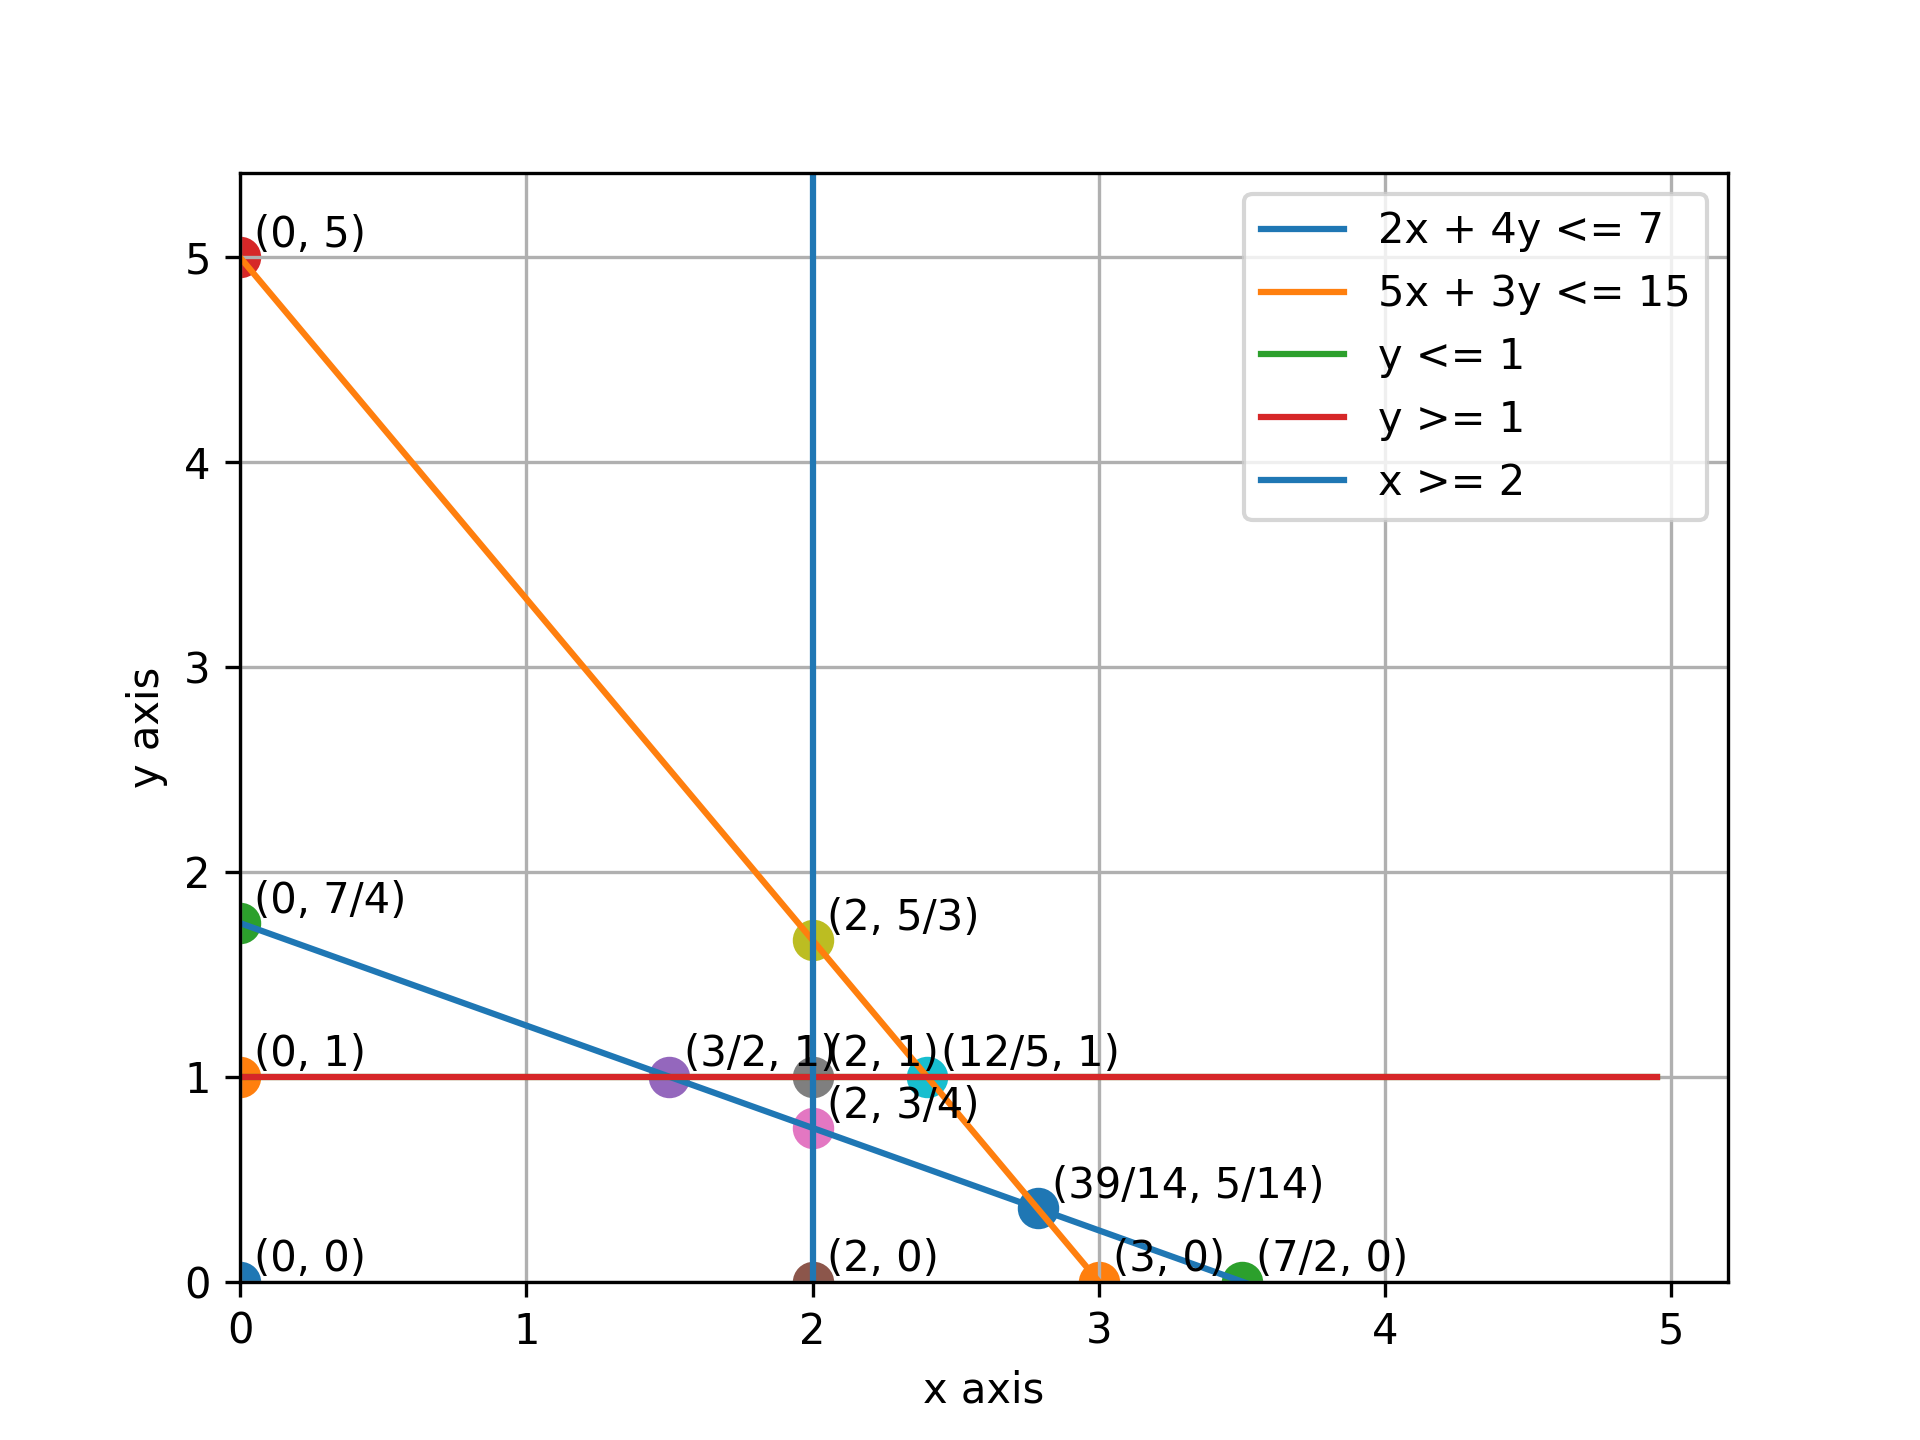
\includegraphics[width=0.6\textwidth]{outputs/ipp1/graph7.png}
\end{center}
Infeasible Solution\\
\begin{align*}
Z=5\end{align*}
\begin{align*}
x=1\end{align*}
\begin{align*}
y=1\end{align*}
\begin{align*}
\text{Maximize} \quad & 7x + 9y\\
\text{subject to} \quad
& -x + 3y\le6\\
& 7x + y\le35\\
& y\le7\\
& x\ge0,\; y\ge0\end{align*}
\begin{align*}
-x + 3y=6\end{align*}
\begin{align*}
7x + y=35\end{align*}
Gauss Elimination:\\
Echelon Form:\\
\begin{align*}
\left(
\begin{array}{cc|c}
-1 & 3 & 6\\
7 & 1 & 35\\
\end{array}
\right)_{2\times 3}
\end{align*}
\begin{align*}
\left(
\begin{array}{cc|c}
-1 & 3 & 6\\
0 & 22 & 77\\
\end{array}
\right)_{2\times 3}
\end{align*}
\begin{align*}
\left(
\begin{array}{cc|c}
-1 & 3 & 6\\
0 & 22 & 77\\
\end{array}
\right)_{2\times 3}
\end{align*}
\begin{align*}
x=\frac{9}{2}\end{align*}
\begin{align*}
y=\frac{7}{2}\end{align*}
\begin{align*}
-x + 3y=6\end{align*}
\begin{align*}
y=7\end{align*}
Gauss Elimination:\\
Echelon Form:\\
\begin{align*}
\left(
\begin{array}{cc|c}
-1 & 3 & 6\\
0 & 1 & 7\\
\end{array}
\right)_{2\times 3}
\end{align*}
\begin{align*}
\left(
\begin{array}{cc|c}
-1 & 3 & 6\\
0 & 1 & 7\\
\end{array}
\right)_{2\times 3}
\end{align*}
\begin{align*}
\left(
\begin{array}{cc|c}
-1 & 3 & 6\\
0 & 1 & 7\\
\end{array}
\right)_{2\times 3}
\end{align*}
\begin{align*}
x=15\end{align*}
\begin{align*}
y=7\end{align*}
\begin{align*}
7x + y=35\end{align*}
\begin{align*}
y=7\end{align*}
Gauss Elimination:\\
Echelon Form:\\
\begin{align*}
\left(
\begin{array}{cc|c}
7 & 1 & 35\\
0 & 1 & 7\\
\end{array}
\right)_{2\times 3}
\end{align*}
\begin{align*}
\left(
\begin{array}{cc|c}
7 & 1 & 35\\
0 & 1 & 7\\
\end{array}
\right)_{2\times 3}
\end{align*}
\begin{align*}
\left(
\begin{array}{cc|c}
7 & 1 & 35\\
0 & 1 & 7\\
\end{array}
\right)_{2\times 3}
\end{align*}
\begin{align*}
x=4\end{align*}
\begin{align*}
y=7\end{align*}
\begin{center}
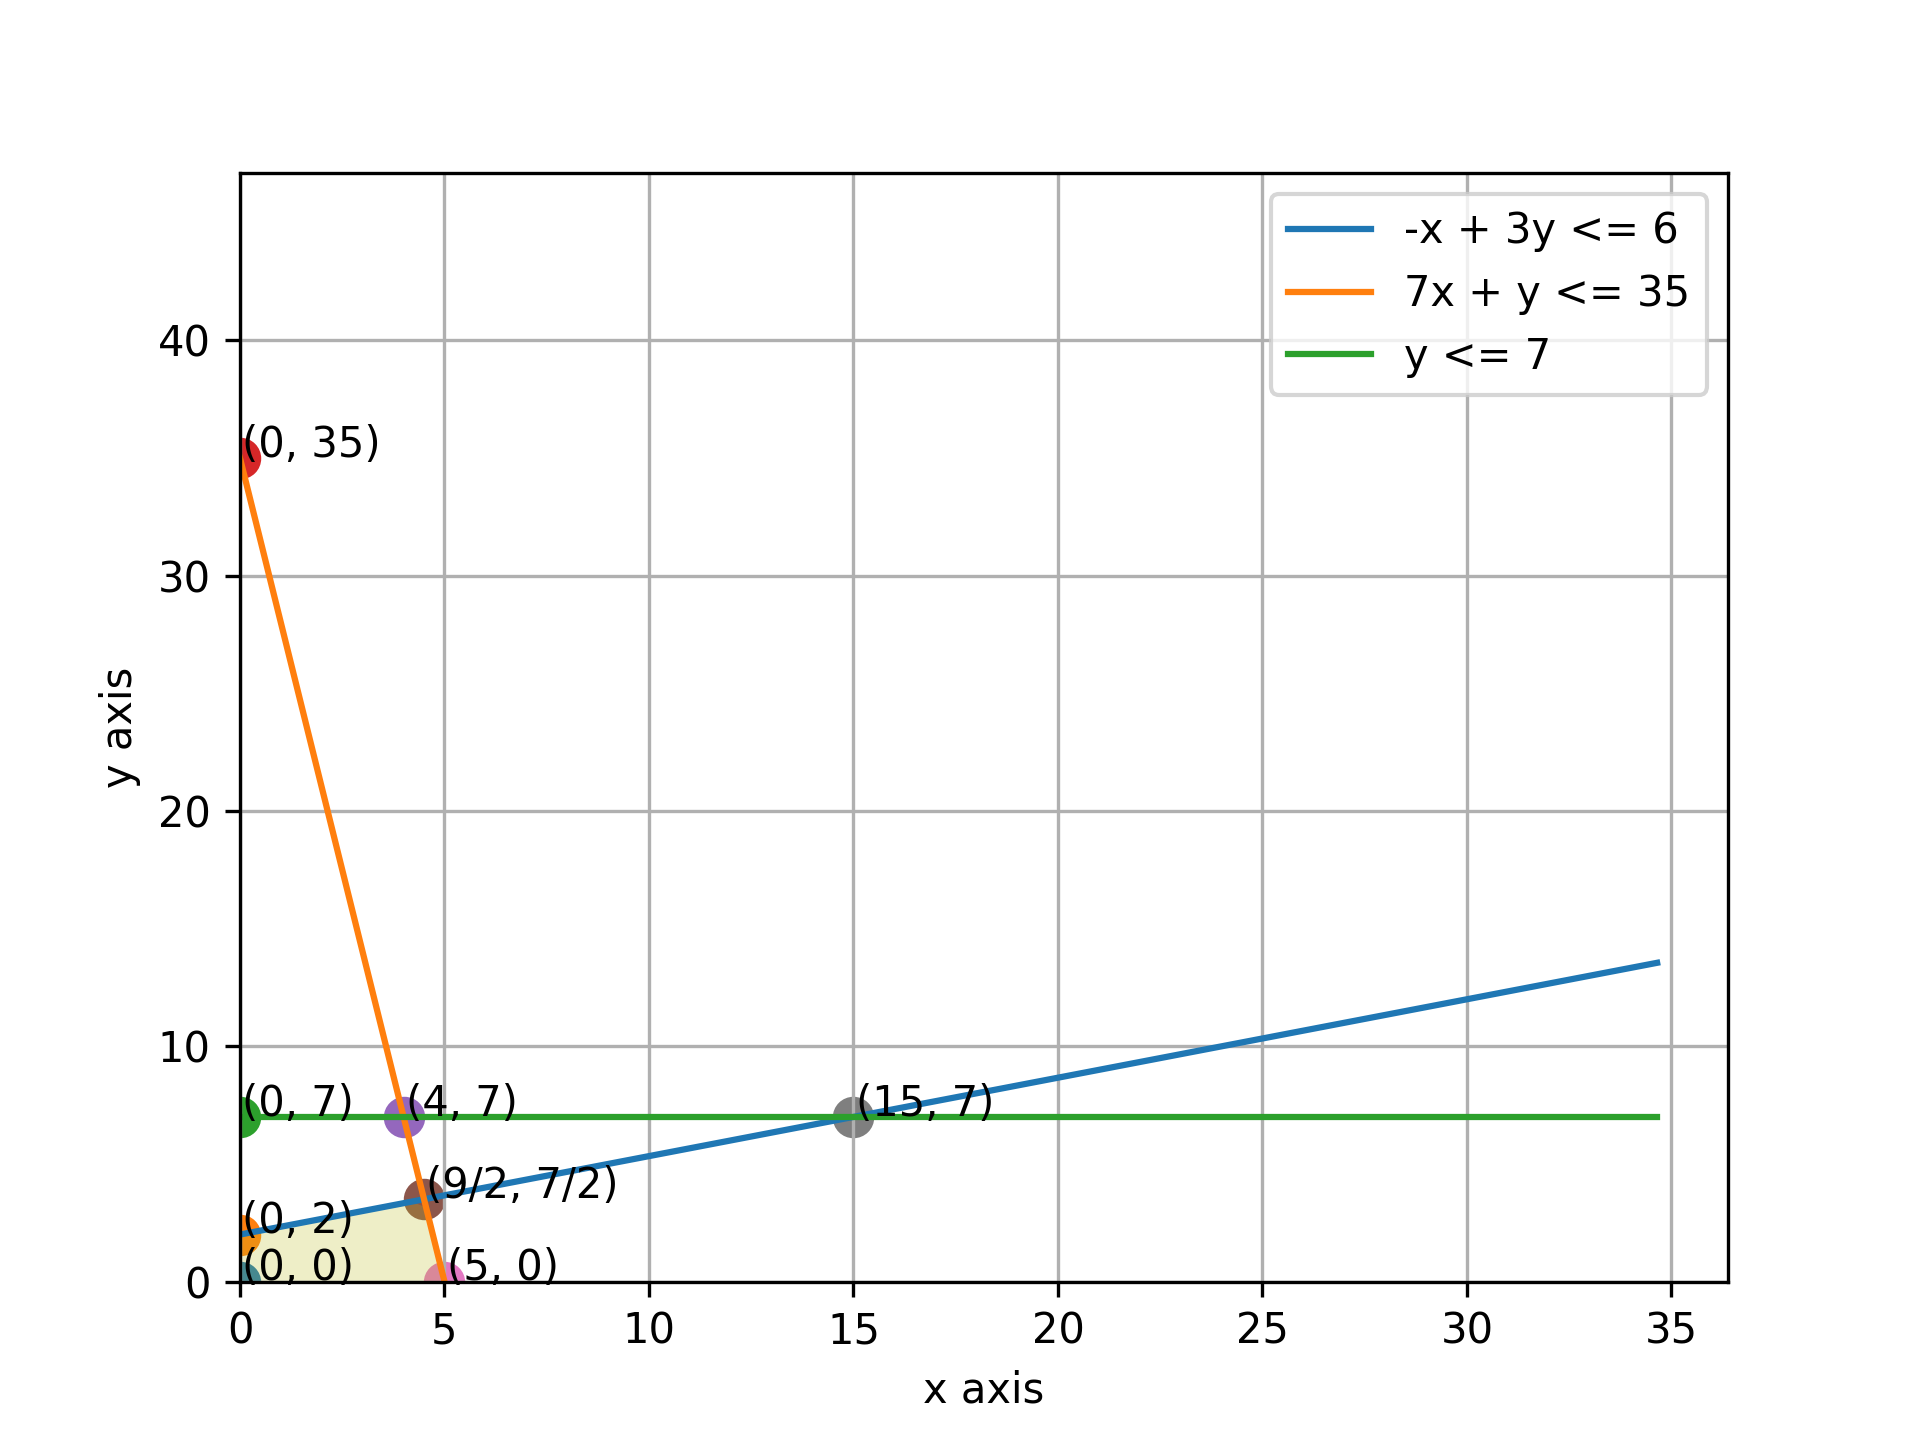
\includegraphics[width=0.6\textwidth]{outputs/ipp2/graph1.png}
\end{center}
\begin{align*}
Z=63\end{align*}
\begin{align*}
x=9\end{align*}
\begin{align*}
y=7\end{align*}
\begin{align*}
\text{Maximize} \quad & 7x + 9y\\
\text{subject to} \quad
& -x + 3y\le6\\
& 7x + y\le35\\
& y\le7\\
& x\le4\\
& x\ge0,\; y\ge0\end{align*}
\begin{align*}
-x + 3y=6\end{align*}
\begin{align*}
7x + y=35\end{align*}
Gauss Elimination:\\
Echelon Form:\\
\begin{align*}
\left(
\begin{array}{cc|c}
-1 & 3 & 6\\
7 & 1 & 35\\
\end{array}
\right)_{2\times 3}
\end{align*}
\begin{align*}
\left(
\begin{array}{cc|c}
-1 & 3 & 6\\
0 & 22 & 77\\
\end{array}
\right)_{2\times 3}
\end{align*}
\begin{align*}
\left(
\begin{array}{cc|c}
-1 & 3 & 6\\
0 & 22 & 77\\
\end{array}
\right)_{2\times 3}
\end{align*}
\begin{align*}
x=\frac{9}{2}\end{align*}
\begin{align*}
y=\frac{7}{2}\end{align*}
\begin{align*}
-x + 3y=6\end{align*}
\begin{align*}
y=7\end{align*}
Gauss Elimination:\\
Echelon Form:\\
\begin{align*}
\left(
\begin{array}{cc|c}
-1 & 3 & 6\\
0 & 1 & 7\\
\end{array}
\right)_{2\times 3}
\end{align*}
\begin{align*}
\left(
\begin{array}{cc|c}
-1 & 3 & 6\\
0 & 1 & 7\\
\end{array}
\right)_{2\times 3}
\end{align*}
\begin{align*}
\left(
\begin{array}{cc|c}
-1 & 3 & 6\\
0 & 1 & 7\\
\end{array}
\right)_{2\times 3}
\end{align*}
\begin{align*}
x=15\end{align*}
\begin{align*}
y=7\end{align*}
\begin{align*}
-x + 3y=6\end{align*}
\begin{align*}
x=4\end{align*}
Gauss Elimination:\\
Echelon Form:\\
\begin{align*}
\left(
\begin{array}{cc|c}
-1 & 3 & 6\\
1 & 0 & 4\\
\end{array}
\right)_{2\times 3}
\end{align*}
\begin{align*}
\left(
\begin{array}{cc|c}
-1 & 3 & 6\\
0 & 3 & 10\\
\end{array}
\right)_{2\times 3}
\end{align*}
\begin{align*}
\left(
\begin{array}{cc|c}
-1 & 3 & 6\\
0 & 3 & 10\\
\end{array}
\right)_{2\times 3}
\end{align*}
\begin{align*}
x=4\end{align*}
\begin{align*}
y=\frac{10}{3}\end{align*}
\begin{align*}
7x + y=35\end{align*}
\begin{align*}
y=7\end{align*}
Gauss Elimination:\\
Echelon Form:\\
\begin{align*}
\left(
\begin{array}{cc|c}
7 & 1 & 35\\
0 & 1 & 7\\
\end{array}
\right)_{2\times 3}
\end{align*}
\begin{align*}
\left(
\begin{array}{cc|c}
7 & 1 & 35\\
0 & 1 & 7\\
\end{array}
\right)_{2\times 3}
\end{align*}
\begin{align*}
\left(
\begin{array}{cc|c}
7 & 1 & 35\\
0 & 1 & 7\\
\end{array}
\right)_{2\times 3}
\end{align*}
\begin{align*}
x=4\end{align*}
\begin{align*}
y=7\end{align*}
\begin{align*}
7x + y=35\end{align*}
\begin{align*}
x=4\end{align*}
Gauss Elimination:\\
Echelon Form:\\
\begin{align*}
\left(
\begin{array}{cc|c}
7 & 1 & 35\\
1 & 0 & 4\\
\end{array}
\right)_{2\times 3}
\end{align*}
\begin{align*}
\left(
\begin{array}{cc|c}
7 & 1 & 35\\
0 & -\frac{1}{7} & -1\\
\end{array}
\right)_{2\times 3}
\end{align*}
\begin{align*}
\left(
\begin{array}{cc|c}
7 & 1 & 35\\
0 & -\frac{1}{7} & -1\\
\end{array}
\right)_{2\times 3}
\end{align*}
\begin{align*}
x=4\end{align*}
\begin{align*}
y=7\end{align*}
\begin{align*}
y=7\end{align*}
\begin{align*}
x=4\end{align*}
Gauss Elimination:\\
Echelon Form:\\
\begin{align*}
\left(
\begin{array}{cc|c}
0 & 1 & 7\\
1 & 0 & 4\\
\end{array}
\right)_{2\times 3}
\end{align*}
\begin{align*}
\left(
\begin{array}{cc|c}
1 & 0 & 4\\
0 & 1 & 7\\
\end{array}
\right)_{2\times 3}
\end{align*}
\begin{align*}
\left(
\begin{array}{cc|c}
1 & 0 & 4\\
0 & 1 & 7\\
\end{array}
\right)_{2\times 3}
\end{align*}
\begin{align*}
x=4\end{align*}
\begin{align*}
y=7\end{align*}
\begin{center}
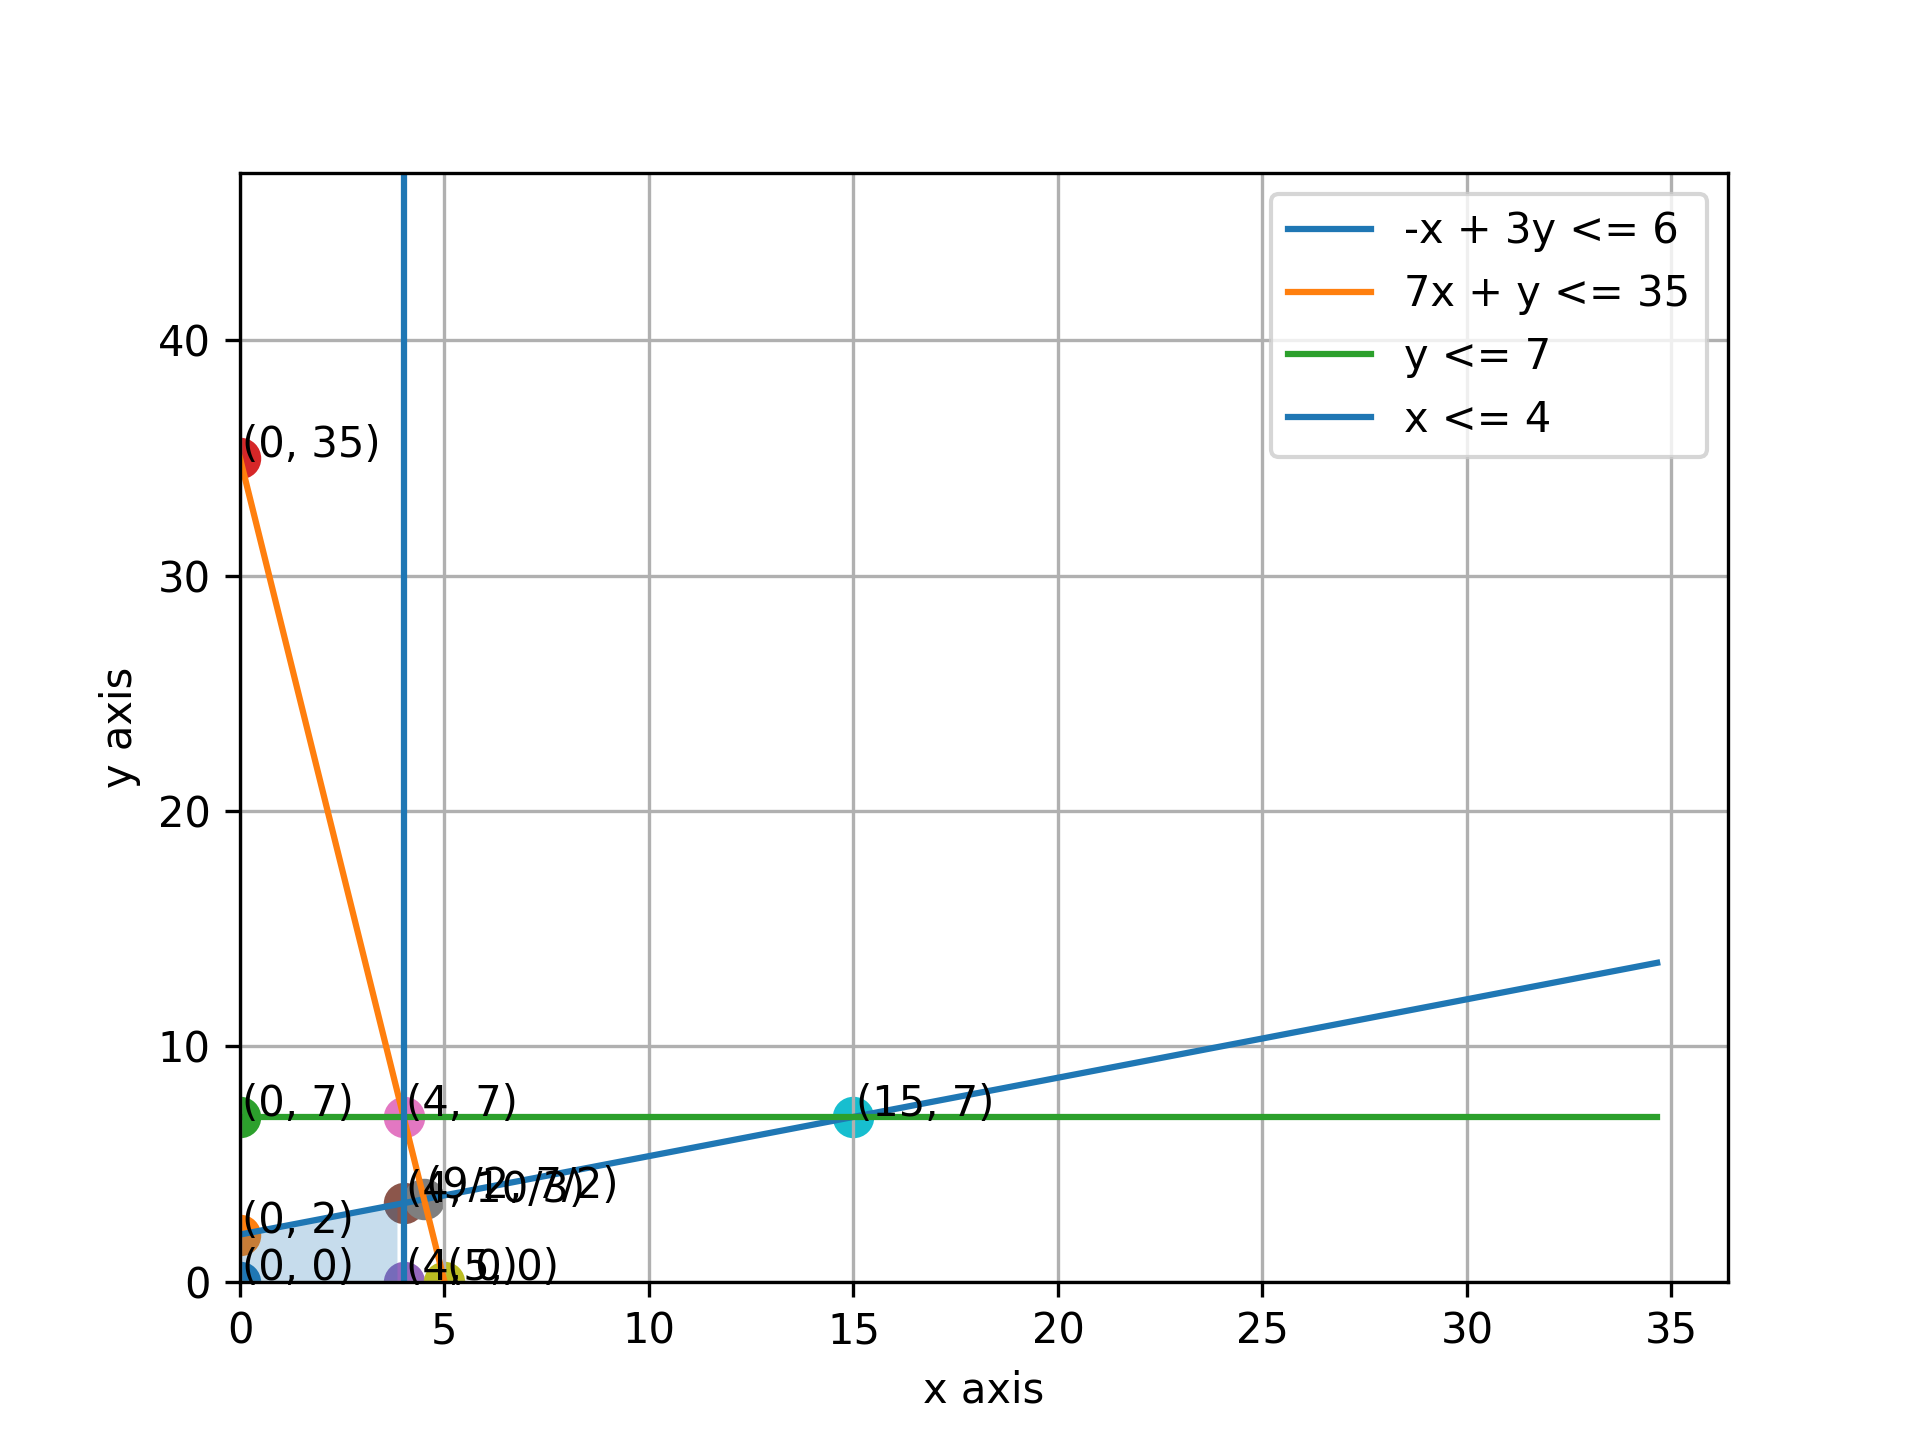
\includegraphics[width=0.6\textwidth]{outputs/ipp2/graph2.png}
\end{center}
\begin{align*}
Z=58\end{align*}
\begin{align*}
x=4\end{align*}
\begin{align*}
y=10\end{align*}
\begin{align*}
\text{Maximize} \quad & 7x + 9y\\
\text{subject to} \quad
& -x + 3y\le6\\
& 7x + y\le35\\
& y\le7\\
& x\ge5\\
& x\ge0,\; y\ge0\end{align*}
\begin{align*}
-x + 3y=6\end{align*}
\begin{align*}
7x + y=35\end{align*}
Gauss Elimination:\\
Echelon Form:\\
\begin{align*}
\left(
\begin{array}{cc|c}
-1 & 3 & 6\\
7 & 1 & 35\\
\end{array}
\right)_{2\times 3}
\end{align*}
\begin{align*}
\left(
\begin{array}{cc|c}
-1 & 3 & 6\\
0 & 22 & 77\\
\end{array}
\right)_{2\times 3}
\end{align*}
\begin{align*}
\left(
\begin{array}{cc|c}
-1 & 3 & 6\\
0 & 22 & 77\\
\end{array}
\right)_{2\times 3}
\end{align*}
\begin{align*}
x=\frac{9}{2}\end{align*}
\begin{align*}
y=\frac{7}{2}\end{align*}
\begin{align*}
-x + 3y=6\end{align*}
\begin{align*}
y=7\end{align*}
Gauss Elimination:\\
Echelon Form:\\
\begin{align*}
\left(
\begin{array}{cc|c}
-1 & 3 & 6\\
0 & 1 & 7\\
\end{array}
\right)_{2\times 3}
\end{align*}
\begin{align*}
\left(
\begin{array}{cc|c}
-1 & 3 & 6\\
0 & 1 & 7\\
\end{array}
\right)_{2\times 3}
\end{align*}
\begin{align*}
\left(
\begin{array}{cc|c}
-1 & 3 & 6\\
0 & 1 & 7\\
\end{array}
\right)_{2\times 3}
\end{align*}
\begin{align*}
x=15\end{align*}
\begin{align*}
y=7\end{align*}
\begin{align*}
-x + 3y=6\end{align*}
\begin{align*}
x=5\end{align*}
Gauss Elimination:\\
Echelon Form:\\
\begin{align*}
\left(
\begin{array}{cc|c}
-1 & 3 & 6\\
1 & 0 & 5\\
\end{array}
\right)_{2\times 3}
\end{align*}
\begin{align*}
\left(
\begin{array}{cc|c}
-1 & 3 & 6\\
0 & 3 & 11\\
\end{array}
\right)_{2\times 3}
\end{align*}
\begin{align*}
\left(
\begin{array}{cc|c}
-1 & 3 & 6\\
0 & 3 & 11\\
\end{array}
\right)_{2\times 3}
\end{align*}
\begin{align*}
x=5\end{align*}
\begin{align*}
y=\frac{11}{3}\end{align*}
\begin{align*}
7x + y=35\end{align*}
\begin{align*}
y=7\end{align*}
Gauss Elimination:\\
Echelon Form:\\
\begin{align*}
\left(
\begin{array}{cc|c}
7 & 1 & 35\\
0 & 1 & 7\\
\end{array}
\right)_{2\times 3}
\end{align*}
\begin{align*}
\left(
\begin{array}{cc|c}
7 & 1 & 35\\
0 & 1 & 7\\
\end{array}
\right)_{2\times 3}
\end{align*}
\begin{align*}
\left(
\begin{array}{cc|c}
7 & 1 & 35\\
0 & 1 & 7\\
\end{array}
\right)_{2\times 3}
\end{align*}
\begin{align*}
x=4\end{align*}
\begin{align*}
y=7\end{align*}
\begin{align*}
7x + y=35\end{align*}
\begin{align*}
x=5\end{align*}
Gauss Elimination:\\
Echelon Form:\\
\begin{align*}
\left(
\begin{array}{cc|c}
7 & 1 & 35\\
1 & 0 & 5\\
\end{array}
\right)_{2\times 3}
\end{align*}
\begin{align*}
\left(
\begin{array}{cc|c}
7 & 1 & 35\\
0 & -\frac{1}{7} & 0\\
\end{array}
\right)_{2\times 3}
\end{align*}
\begin{align*}
\left(
\begin{array}{cc|c}
7 & 1 & 35\\
0 & -\frac{1}{7} & 0\\
\end{array}
\right)_{2\times 3}
\end{align*}
\begin{align*}
x=5\end{align*}
\begin{align*}
y=0\end{align*}
\begin{align*}
y=7\end{align*}
\begin{align*}
x=5\end{align*}
Gauss Elimination:\\
Echelon Form:\\
\begin{align*}
\left(
\begin{array}{cc|c}
0 & 1 & 7\\
1 & 0 & 5\\
\end{array}
\right)_{2\times 3}
\end{align*}
\begin{align*}
\left(
\begin{array}{cc|c}
1 & 0 & 5\\
0 & 1 & 7\\
\end{array}
\right)_{2\times 3}
\end{align*}
\begin{align*}
\left(
\begin{array}{cc|c}
1 & 0 & 5\\
0 & 1 & 7\\
\end{array}
\right)_{2\times 3}
\end{align*}
\begin{align*}
x=5\end{align*}
\begin{align*}
y=7\end{align*}
\begin{center}
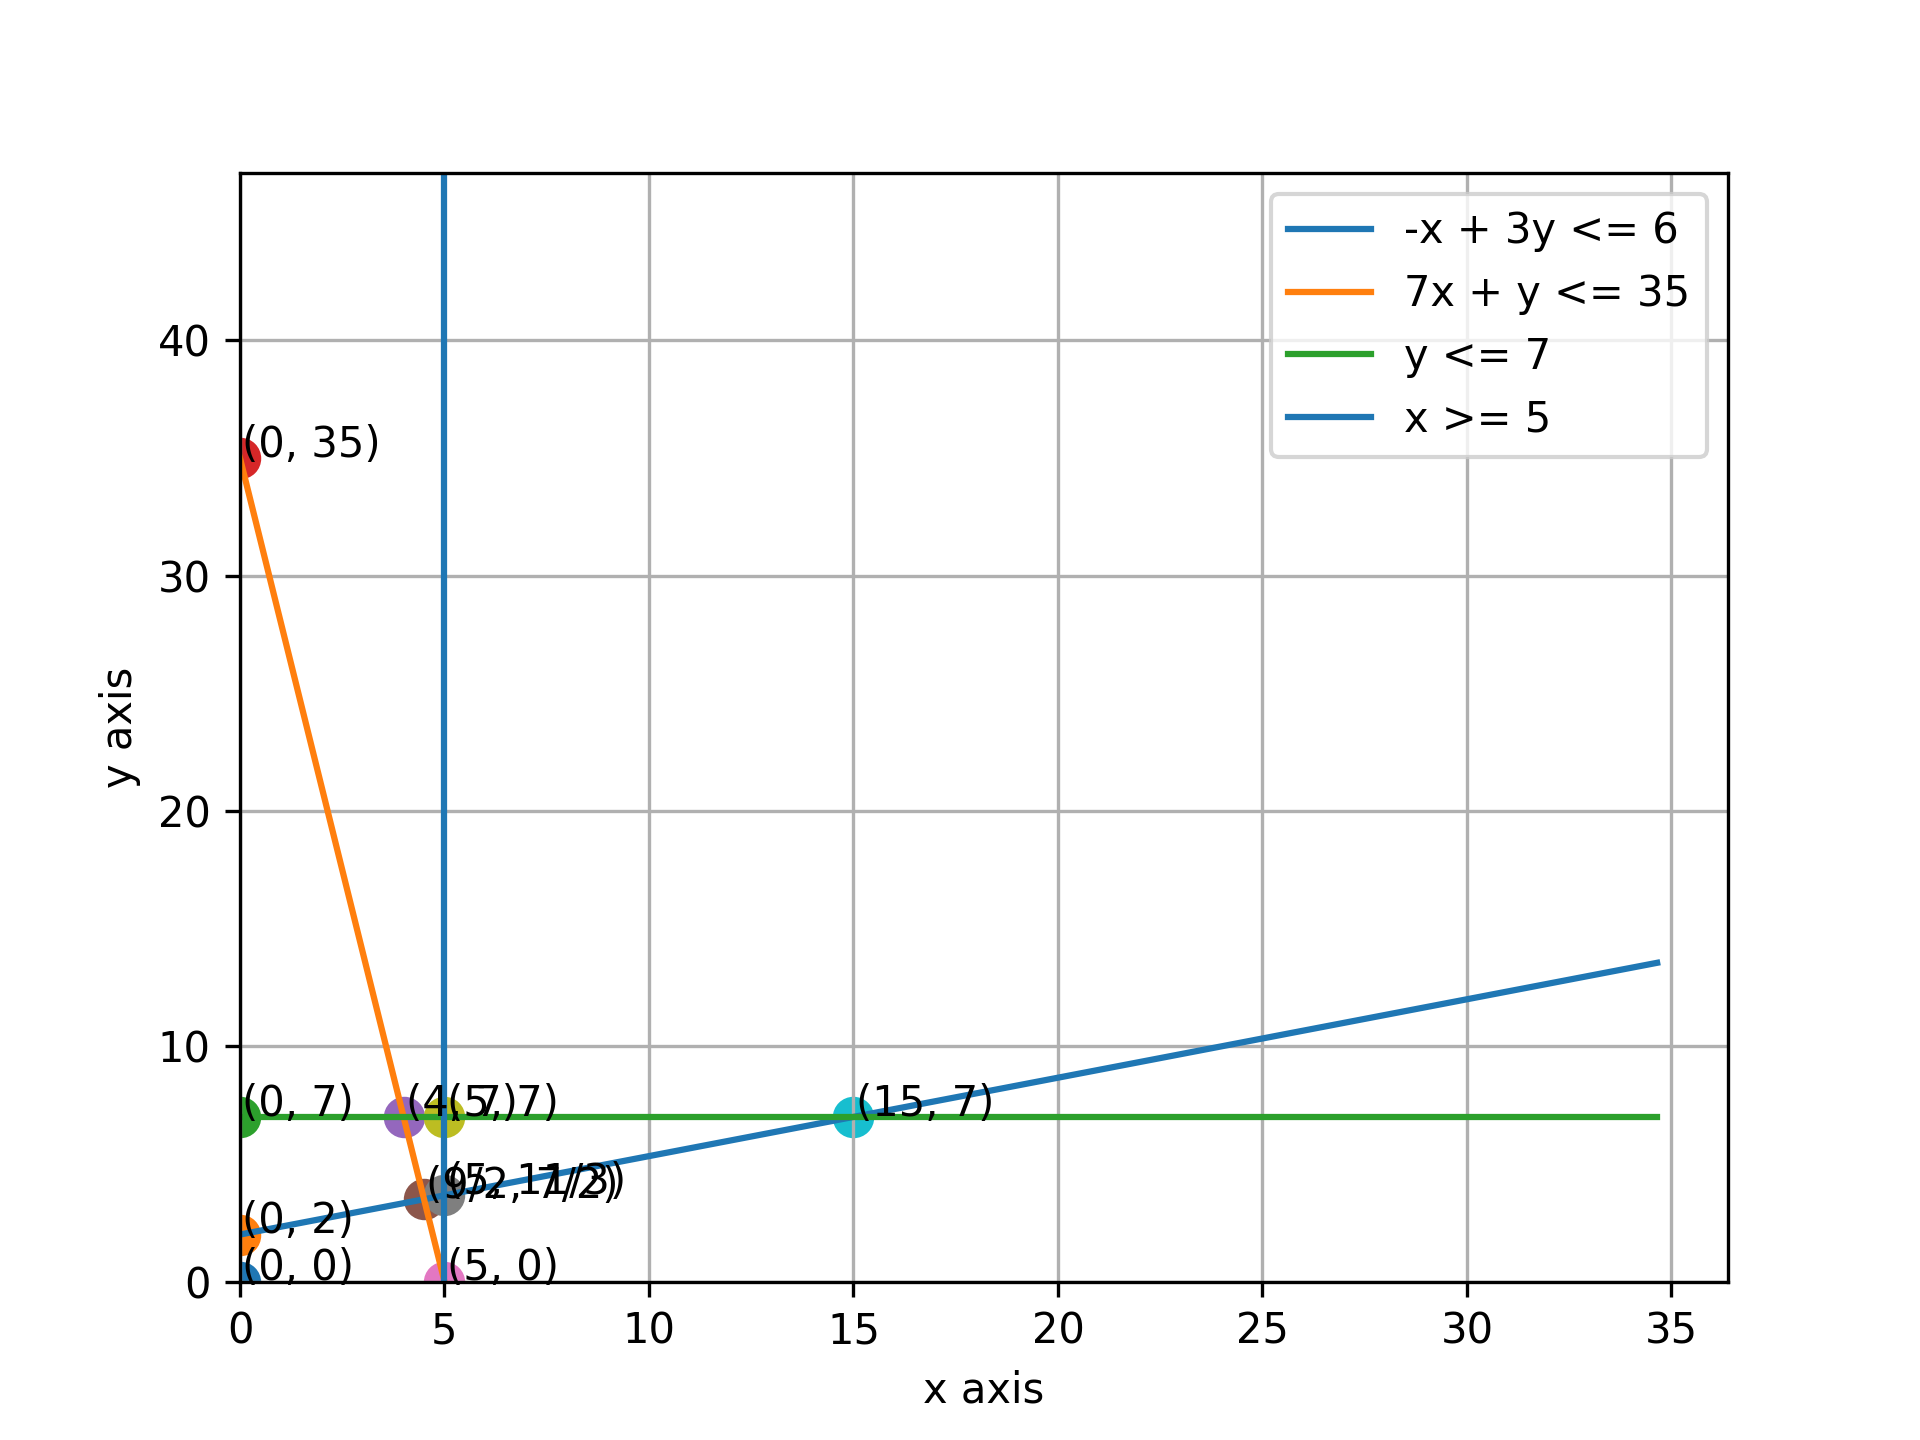
\includegraphics[width=0.6\textwidth]{outputs/ipp2/graph3.png}
\end{center}
\begin{align*}
Z=35\end{align*}
\begin{align*}
x=5\end{align*}
\begin{align*}
y=0\end{align*}
\begin{align*}
\text{Maximize} \quad & 7x + 9y\\
\text{subject to} \quad
& -x + 3y\le6\\
& 7x + y\le35\\
& y\le7\\
& x\le4\\
& y\le3\\
& x\ge0,\; y\ge0\end{align*}
\begin{align*}
-x + 3y=6\end{align*}
\begin{align*}
7x + y=35\end{align*}
Gauss Elimination:\\
Echelon Form:\\
\begin{align*}
\left(
\begin{array}{cc|c}
-1 & 3 & 6\\
7 & 1 & 35\\
\end{array}
\right)_{2\times 3}
\end{align*}
\begin{align*}
\left(
\begin{array}{cc|c}
-1 & 3 & 6\\
0 & 22 & 77\\
\end{array}
\right)_{2\times 3}
\end{align*}
\begin{align*}
\left(
\begin{array}{cc|c}
-1 & 3 & 6\\
0 & 22 & 77\\
\end{array}
\right)_{2\times 3}
\end{align*}
\begin{align*}
x=\frac{9}{2}\end{align*}
\begin{align*}
y=\frac{7}{2}\end{align*}
\begin{align*}
-x + 3y=6\end{align*}
\begin{align*}
y=7\end{align*}
Gauss Elimination:\\
Echelon Form:\\
\begin{align*}
\left(
\begin{array}{cc|c}
-1 & 3 & 6\\
0 & 1 & 7\\
\end{array}
\right)_{2\times 3}
\end{align*}
\begin{align*}
\left(
\begin{array}{cc|c}
-1 & 3 & 6\\
0 & 1 & 7\\
\end{array}
\right)_{2\times 3}
\end{align*}
\begin{align*}
\left(
\begin{array}{cc|c}
-1 & 3 & 6\\
0 & 1 & 7\\
\end{array}
\right)_{2\times 3}
\end{align*}
\begin{align*}
x=15\end{align*}
\begin{align*}
y=7\end{align*}
\begin{align*}
-x + 3y=6\end{align*}
\begin{align*}
x=4\end{align*}
Gauss Elimination:\\
Echelon Form:\\
\begin{align*}
\left(
\begin{array}{cc|c}
-1 & 3 & 6\\
1 & 0 & 4\\
\end{array}
\right)_{2\times 3}
\end{align*}
\begin{align*}
\left(
\begin{array}{cc|c}
-1 & 3 & 6\\
0 & 3 & 10\\
\end{array}
\right)_{2\times 3}
\end{align*}
\begin{align*}
\left(
\begin{array}{cc|c}
-1 & 3 & 6\\
0 & 3 & 10\\
\end{array}
\right)_{2\times 3}
\end{align*}
\begin{align*}
x=4\end{align*}
\begin{align*}
y=\frac{10}{3}\end{align*}
\begin{align*}
-x + 3y=6\end{align*}
\begin{align*}
y=3\end{align*}
Gauss Elimination:\\
Echelon Form:\\
\begin{align*}
\left(
\begin{array}{cc|c}
-1 & 3 & 6\\
0 & 1 & 3\\
\end{array}
\right)_{2\times 3}
\end{align*}
\begin{align*}
\left(
\begin{array}{cc|c}
-1 & 3 & 6\\
0 & 1 & 3\\
\end{array}
\right)_{2\times 3}
\end{align*}
\begin{align*}
\left(
\begin{array}{cc|c}
-1 & 3 & 6\\
0 & 1 & 3\\
\end{array}
\right)_{2\times 3}
\end{align*}
\begin{align*}
x=3\end{align*}
\begin{align*}
y=3\end{align*}
\begin{align*}
7x + y=35\end{align*}
\begin{align*}
y=7\end{align*}
Gauss Elimination:\\
Echelon Form:\\
\begin{align*}
\left(
\begin{array}{cc|c}
7 & 1 & 35\\
0 & 1 & 7\\
\end{array}
\right)_{2\times 3}
\end{align*}
\begin{align*}
\left(
\begin{array}{cc|c}
7 & 1 & 35\\
0 & 1 & 7\\
\end{array}
\right)_{2\times 3}
\end{align*}
\begin{align*}
\left(
\begin{array}{cc|c}
7 & 1 & 35\\
0 & 1 & 7\\
\end{array}
\right)_{2\times 3}
\end{align*}
\begin{align*}
x=4\end{align*}
\begin{align*}
y=7\end{align*}
\begin{align*}
7x + y=35\end{align*}
\begin{align*}
x=4\end{align*}
Gauss Elimination:\\
Echelon Form:\\
\begin{align*}
\left(
\begin{array}{cc|c}
7 & 1 & 35\\
1 & 0 & 4\\
\end{array}
\right)_{2\times 3}
\end{align*}
\begin{align*}
\left(
\begin{array}{cc|c}
7 & 1 & 35\\
0 & -\frac{1}{7} & -1\\
\end{array}
\right)_{2\times 3}
\end{align*}
\begin{align*}
\left(
\begin{array}{cc|c}
7 & 1 & 35\\
0 & -\frac{1}{7} & -1\\
\end{array}
\right)_{2\times 3}
\end{align*}
\begin{align*}
x=4\end{align*}
\begin{align*}
y=7\end{align*}
\begin{align*}
7x + y=35\end{align*}
\begin{align*}
y=3\end{align*}
Gauss Elimination:\\
Echelon Form:\\
\begin{align*}
\left(
\begin{array}{cc|c}
7 & 1 & 35\\
0 & 1 & 3\\
\end{array}
\right)_{2\times 3}
\end{align*}
\begin{align*}
\left(
\begin{array}{cc|c}
7 & 1 & 35\\
0 & 1 & 3\\
\end{array}
\right)_{2\times 3}
\end{align*}
\begin{align*}
\left(
\begin{array}{cc|c}
7 & 1 & 35\\
0 & 1 & 3\\
\end{array}
\right)_{2\times 3}
\end{align*}
\begin{align*}
x=\frac{32}{7}\end{align*}
\begin{align*}
y=3\end{align*}
\begin{align*}
y=7\end{align*}
\begin{align*}
x=4\end{align*}
Gauss Elimination:\\
Echelon Form:\\
\begin{align*}
\left(
\begin{array}{cc|c}
0 & 1 & 7\\
1 & 0 & 4\\
\end{array}
\right)_{2\times 3}
\end{align*}
\begin{align*}
\left(
\begin{array}{cc|c}
1 & 0 & 4\\
0 & 1 & 7\\
\end{array}
\right)_{2\times 3}
\end{align*}
\begin{align*}
\left(
\begin{array}{cc|c}
1 & 0 & 4\\
0 & 1 & 7\\
\end{array}
\right)_{2\times 3}
\end{align*}
\begin{align*}
x=4\end{align*}
\begin{align*}
y=7\end{align*}
\begin{align*}
y=7\end{align*}
\begin{align*}
y=3\end{align*}
Gauss Elimination:\\
Echelon Form:\\
\begin{align*}
\left(
\begin{array}{c|c}
1 & 7\\
1 & 3\\
\end{array}
\right)_{2\times 2}
\end{align*}
\begin{align*}
\left(
\begin{array}{c|c}
1 & 7\\
0 & -4\\
\end{array}
\right)_{2\times 2}
\end{align*}
\begin{align*}
\left(
\begin{array}{c|c}
1 & 7\\
0 & -4\\
\end{array}
\right)_{2\times 2}
\end{align*}
No solution\\
\begin{align*}
x=4\end{align*}
\begin{align*}
y=3\end{align*}
Gauss Elimination:\\
Echelon Form:\\
\begin{align*}
\left(
\begin{array}{cc|c}
1 & 0 & 4\\
0 & 1 & 3\\
\end{array}
\right)_{2\times 3}
\end{align*}
\begin{align*}
\left(
\begin{array}{cc|c}
1 & 0 & 4\\
0 & 1 & 3\\
\end{array}
\right)_{2\times 3}
\end{align*}
\begin{align*}
\left(
\begin{array}{cc|c}
1 & 0 & 4\\
0 & 1 & 3\\
\end{array}
\right)_{2\times 3}
\end{align*}
\begin{align*}
x=4\end{align*}
\begin{align*}
y=3\end{align*}
\begin{center}
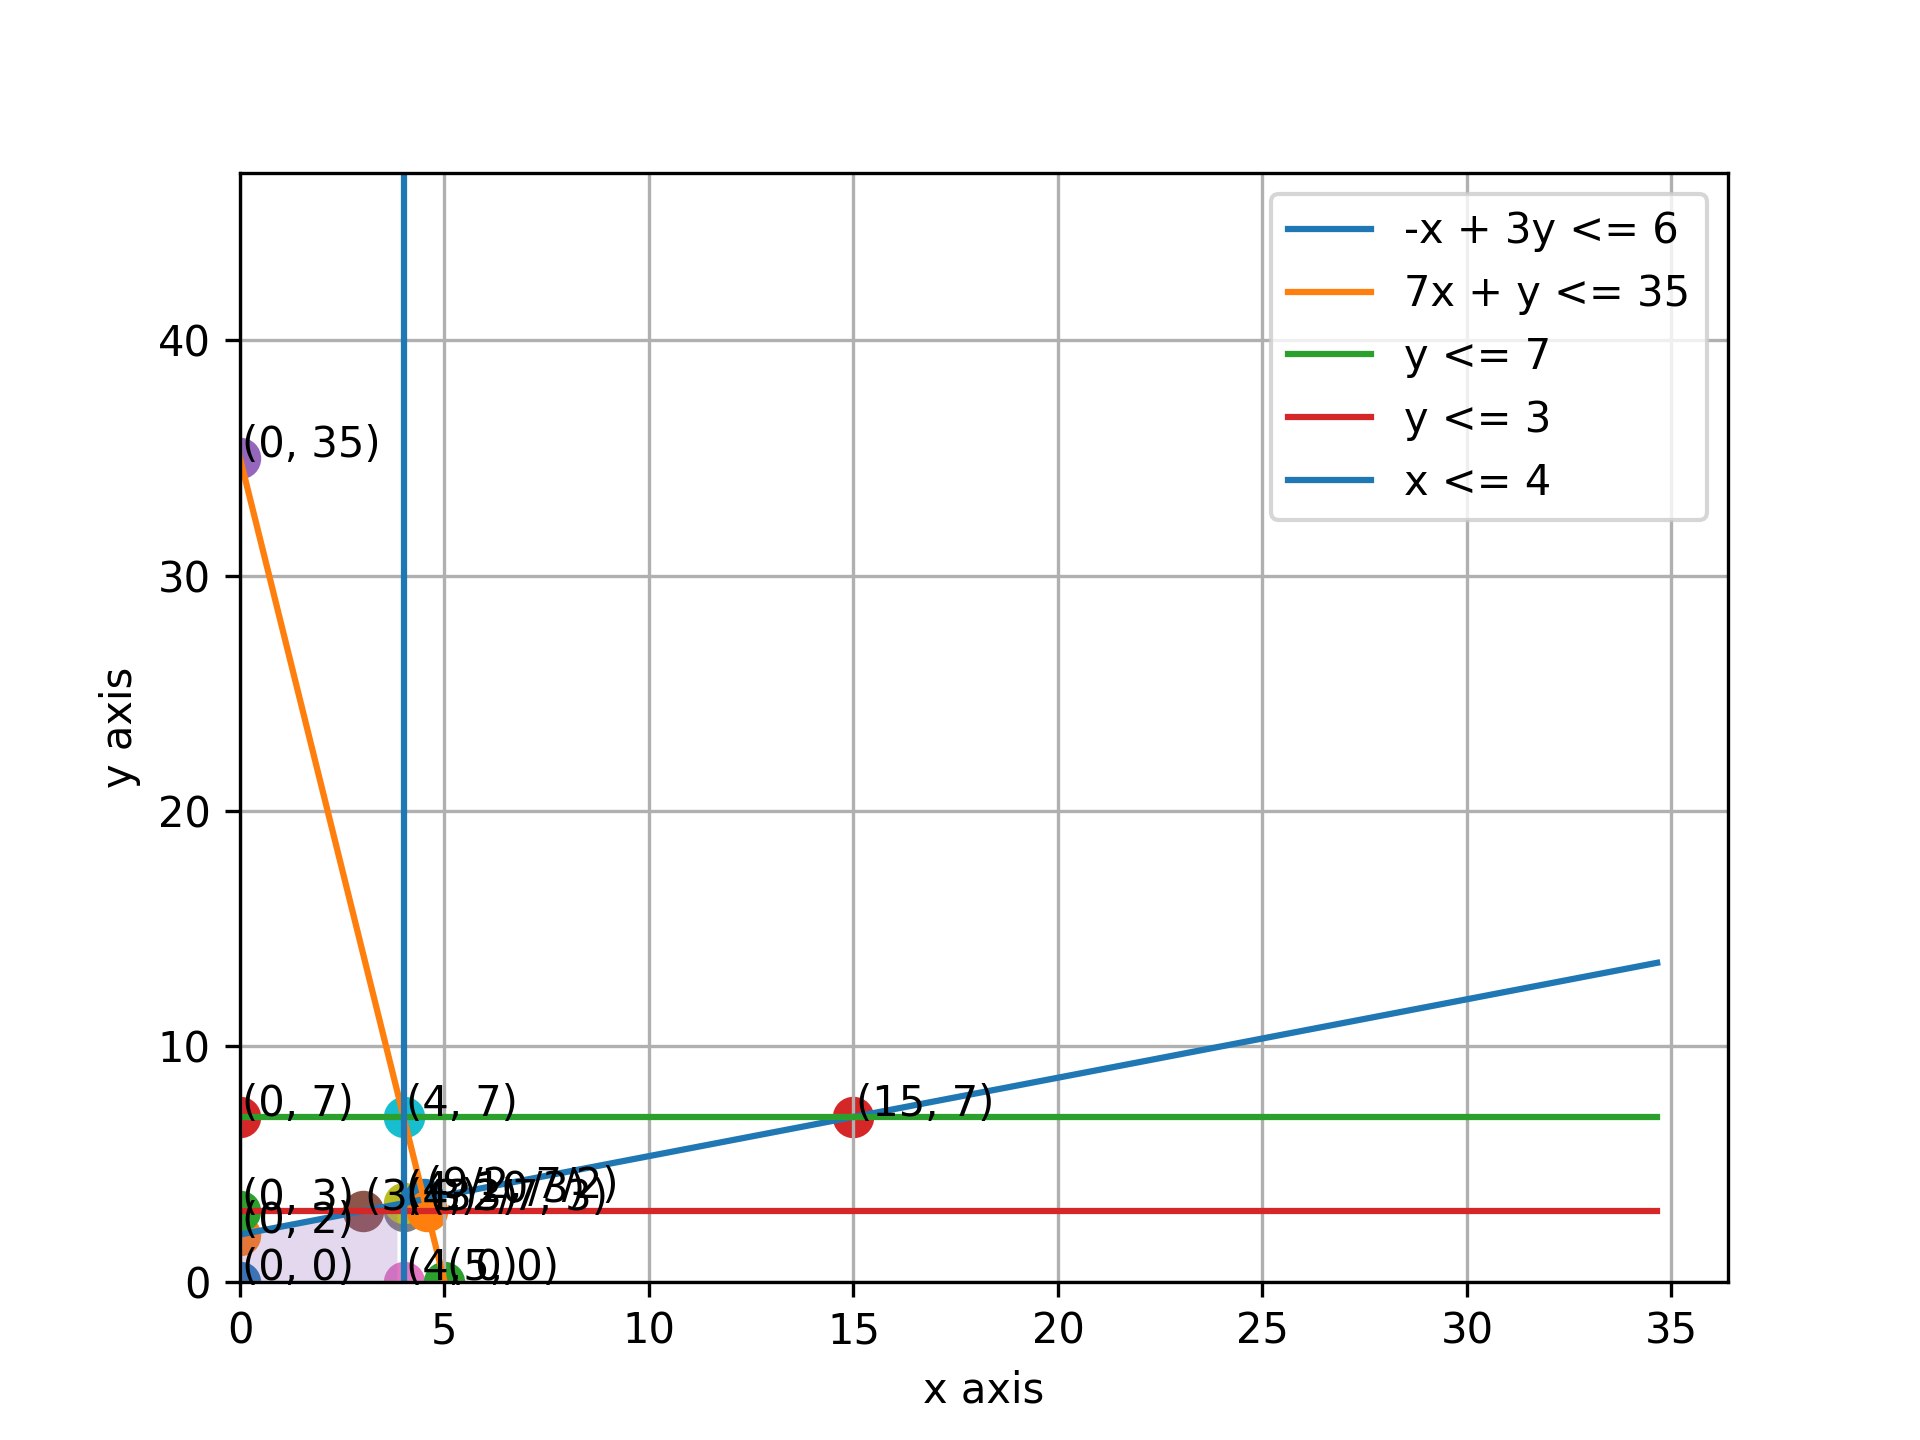
\includegraphics[width=0.6\textwidth]{outputs/ipp2/graph4.png}
\end{center}
\begin{align*}
Z=55\end{align*}
\begin{align*}
x=4\end{align*}
\begin{align*}
y=3\end{align*}
\begin{align*}
\text{Maximize} \quad & 7x + 9y\\
\text{subject to} \quad
& -x + 3y\le6\\
& 7x + y\le35\\
& y\le7\\
& x\le4\\
& y\ge4\\
& x\ge0,\; y\ge0\end{align*}
\begin{align*}
-x + 3y=6\end{align*}
\begin{align*}
7x + y=35\end{align*}
Gauss Elimination:\\
Echelon Form:\\
\begin{align*}
\left(
\begin{array}{cc|c}
-1 & 3 & 6\\
7 & 1 & 35\\
\end{array}
\right)_{2\times 3}
\end{align*}
\begin{align*}
\left(
\begin{array}{cc|c}
-1 & 3 & 6\\
0 & 22 & 77\\
\end{array}
\right)_{2\times 3}
\end{align*}
\begin{align*}
\left(
\begin{array}{cc|c}
-1 & 3 & 6\\
0 & 22 & 77\\
\end{array}
\right)_{2\times 3}
\end{align*}
\begin{align*}
x=\frac{9}{2}\end{align*}
\begin{align*}
y=\frac{7}{2}\end{align*}
\begin{align*}
-x + 3y=6\end{align*}
\begin{align*}
y=7\end{align*}
Gauss Elimination:\\
Echelon Form:\\
\begin{align*}
\left(
\begin{array}{cc|c}
-1 & 3 & 6\\
0 & 1 & 7\\
\end{array}
\right)_{2\times 3}
\end{align*}
\begin{align*}
\left(
\begin{array}{cc|c}
-1 & 3 & 6\\
0 & 1 & 7\\
\end{array}
\right)_{2\times 3}
\end{align*}
\begin{align*}
\left(
\begin{array}{cc|c}
-1 & 3 & 6\\
0 & 1 & 7\\
\end{array}
\right)_{2\times 3}
\end{align*}
\begin{align*}
x=15\end{align*}
\begin{align*}
y=7\end{align*}
\begin{align*}
-x + 3y=6\end{align*}
\begin{align*}
x=4\end{align*}
Gauss Elimination:\\
Echelon Form:\\
\begin{align*}
\left(
\begin{array}{cc|c}
-1 & 3 & 6\\
1 & 0 & 4\\
\end{array}
\right)_{2\times 3}
\end{align*}
\begin{align*}
\left(
\begin{array}{cc|c}
-1 & 3 & 6\\
0 & 3 & 10\\
\end{array}
\right)_{2\times 3}
\end{align*}
\begin{align*}
\left(
\begin{array}{cc|c}
-1 & 3 & 6\\
0 & 3 & 10\\
\end{array}
\right)_{2\times 3}
\end{align*}
\begin{align*}
x=4\end{align*}
\begin{align*}
y=\frac{10}{3}\end{align*}
\begin{align*}
-x + 3y=6\end{align*}
\begin{align*}
y=4\end{align*}
Gauss Elimination:\\
Echelon Form:\\
\begin{align*}
\left(
\begin{array}{cc|c}
-1 & 3 & 6\\
0 & 1 & 4\\
\end{array}
\right)_{2\times 3}
\end{align*}
\begin{align*}
\left(
\begin{array}{cc|c}
-1 & 3 & 6\\
0 & 1 & 4\\
\end{array}
\right)_{2\times 3}
\end{align*}
\begin{align*}
\left(
\begin{array}{cc|c}
-1 & 3 & 6\\
0 & 1 & 4\\
\end{array}
\right)_{2\times 3}
\end{align*}
\begin{align*}
x=6\end{align*}
\begin{align*}
y=4\end{align*}
\begin{align*}
7x + y=35\end{align*}
\begin{align*}
y=7\end{align*}
Gauss Elimination:\\
Echelon Form:\\
\begin{align*}
\left(
\begin{array}{cc|c}
7 & 1 & 35\\
0 & 1 & 7\\
\end{array}
\right)_{2\times 3}
\end{align*}
\begin{align*}
\left(
\begin{array}{cc|c}
7 & 1 & 35\\
0 & 1 & 7\\
\end{array}
\right)_{2\times 3}
\end{align*}
\begin{align*}
\left(
\begin{array}{cc|c}
7 & 1 & 35\\
0 & 1 & 7\\
\end{array}
\right)_{2\times 3}
\end{align*}
\begin{align*}
x=4\end{align*}
\begin{align*}
y=7\end{align*}
\begin{align*}
7x + y=35\end{align*}
\begin{align*}
x=4\end{align*}
Gauss Elimination:\\
Echelon Form:\\
\begin{align*}
\left(
\begin{array}{cc|c}
7 & 1 & 35\\
1 & 0 & 4\\
\end{array}
\right)_{2\times 3}
\end{align*}
\begin{align*}
\left(
\begin{array}{cc|c}
7 & 1 & 35\\
0 & -\frac{1}{7} & -1\\
\end{array}
\right)_{2\times 3}
\end{align*}
\begin{align*}
\left(
\begin{array}{cc|c}
7 & 1 & 35\\
0 & -\frac{1}{7} & -1\\
\end{array}
\right)_{2\times 3}
\end{align*}
\begin{align*}
x=4\end{align*}
\begin{align*}
y=7\end{align*}
\begin{align*}
7x + y=35\end{align*}
\begin{align*}
y=4\end{align*}
Gauss Elimination:\\
Echelon Form:\\
\begin{align*}
\left(
\begin{array}{cc|c}
7 & 1 & 35\\
0 & 1 & 4\\
\end{array}
\right)_{2\times 3}
\end{align*}
\begin{align*}
\left(
\begin{array}{cc|c}
7 & 1 & 35\\
0 & 1 & 4\\
\end{array}
\right)_{2\times 3}
\end{align*}
\begin{align*}
\left(
\begin{array}{cc|c}
7 & 1 & 35\\
0 & 1 & 4\\
\end{array}
\right)_{2\times 3}
\end{align*}
\begin{align*}
x=\frac{31}{7}\end{align*}
\begin{align*}
y=4\end{align*}
\begin{align*}
y=7\end{align*}
\begin{align*}
x=4\end{align*}
Gauss Elimination:\\
Echelon Form:\\
\begin{align*}
\left(
\begin{array}{cc|c}
0 & 1 & 7\\
1 & 0 & 4\\
\end{array}
\right)_{2\times 3}
\end{align*}
\begin{align*}
\left(
\begin{array}{cc|c}
1 & 0 & 4\\
0 & 1 & 7\\
\end{array}
\right)_{2\times 3}
\end{align*}
\begin{align*}
\left(
\begin{array}{cc|c}
1 & 0 & 4\\
0 & 1 & 7\\
\end{array}
\right)_{2\times 3}
\end{align*}
\begin{align*}
x=4\end{align*}
\begin{align*}
y=7\end{align*}
\begin{align*}
y=7\end{align*}
\begin{align*}
y=4\end{align*}
Gauss Elimination:\\
Echelon Form:\\
\begin{align*}
\left(
\begin{array}{c|c}
1 & 7\\
1 & 4\\
\end{array}
\right)_{2\times 2}
\end{align*}
\begin{align*}
\left(
\begin{array}{c|c}
1 & 7\\
0 & -3\\
\end{array}
\right)_{2\times 2}
\end{align*}
\begin{align*}
\left(
\begin{array}{c|c}
1 & 7\\
0 & -3\\
\end{array}
\right)_{2\times 2}
\end{align*}
No solution\\
\begin{align*}
x=4\end{align*}
\begin{align*}
y=4\end{align*}
Gauss Elimination:\\
Echelon Form:\\
\begin{align*}
\left(
\begin{array}{cc|c}
1 & 0 & 4\\
0 & 1 & 4\\
\end{array}
\right)_{2\times 3}
\end{align*}
\begin{align*}
\left(
\begin{array}{cc|c}
1 & 0 & 4\\
0 & 1 & 4\\
\end{array}
\right)_{2\times 3}
\end{align*}
\begin{align*}
\left(
\begin{array}{cc|c}
1 & 0 & 4\\
0 & 1 & 4\\
\end{array}
\right)_{2\times 3}
\end{align*}
\begin{align*}
x=4\end{align*}
\begin{align*}
y=4\end{align*}
\begin{center}
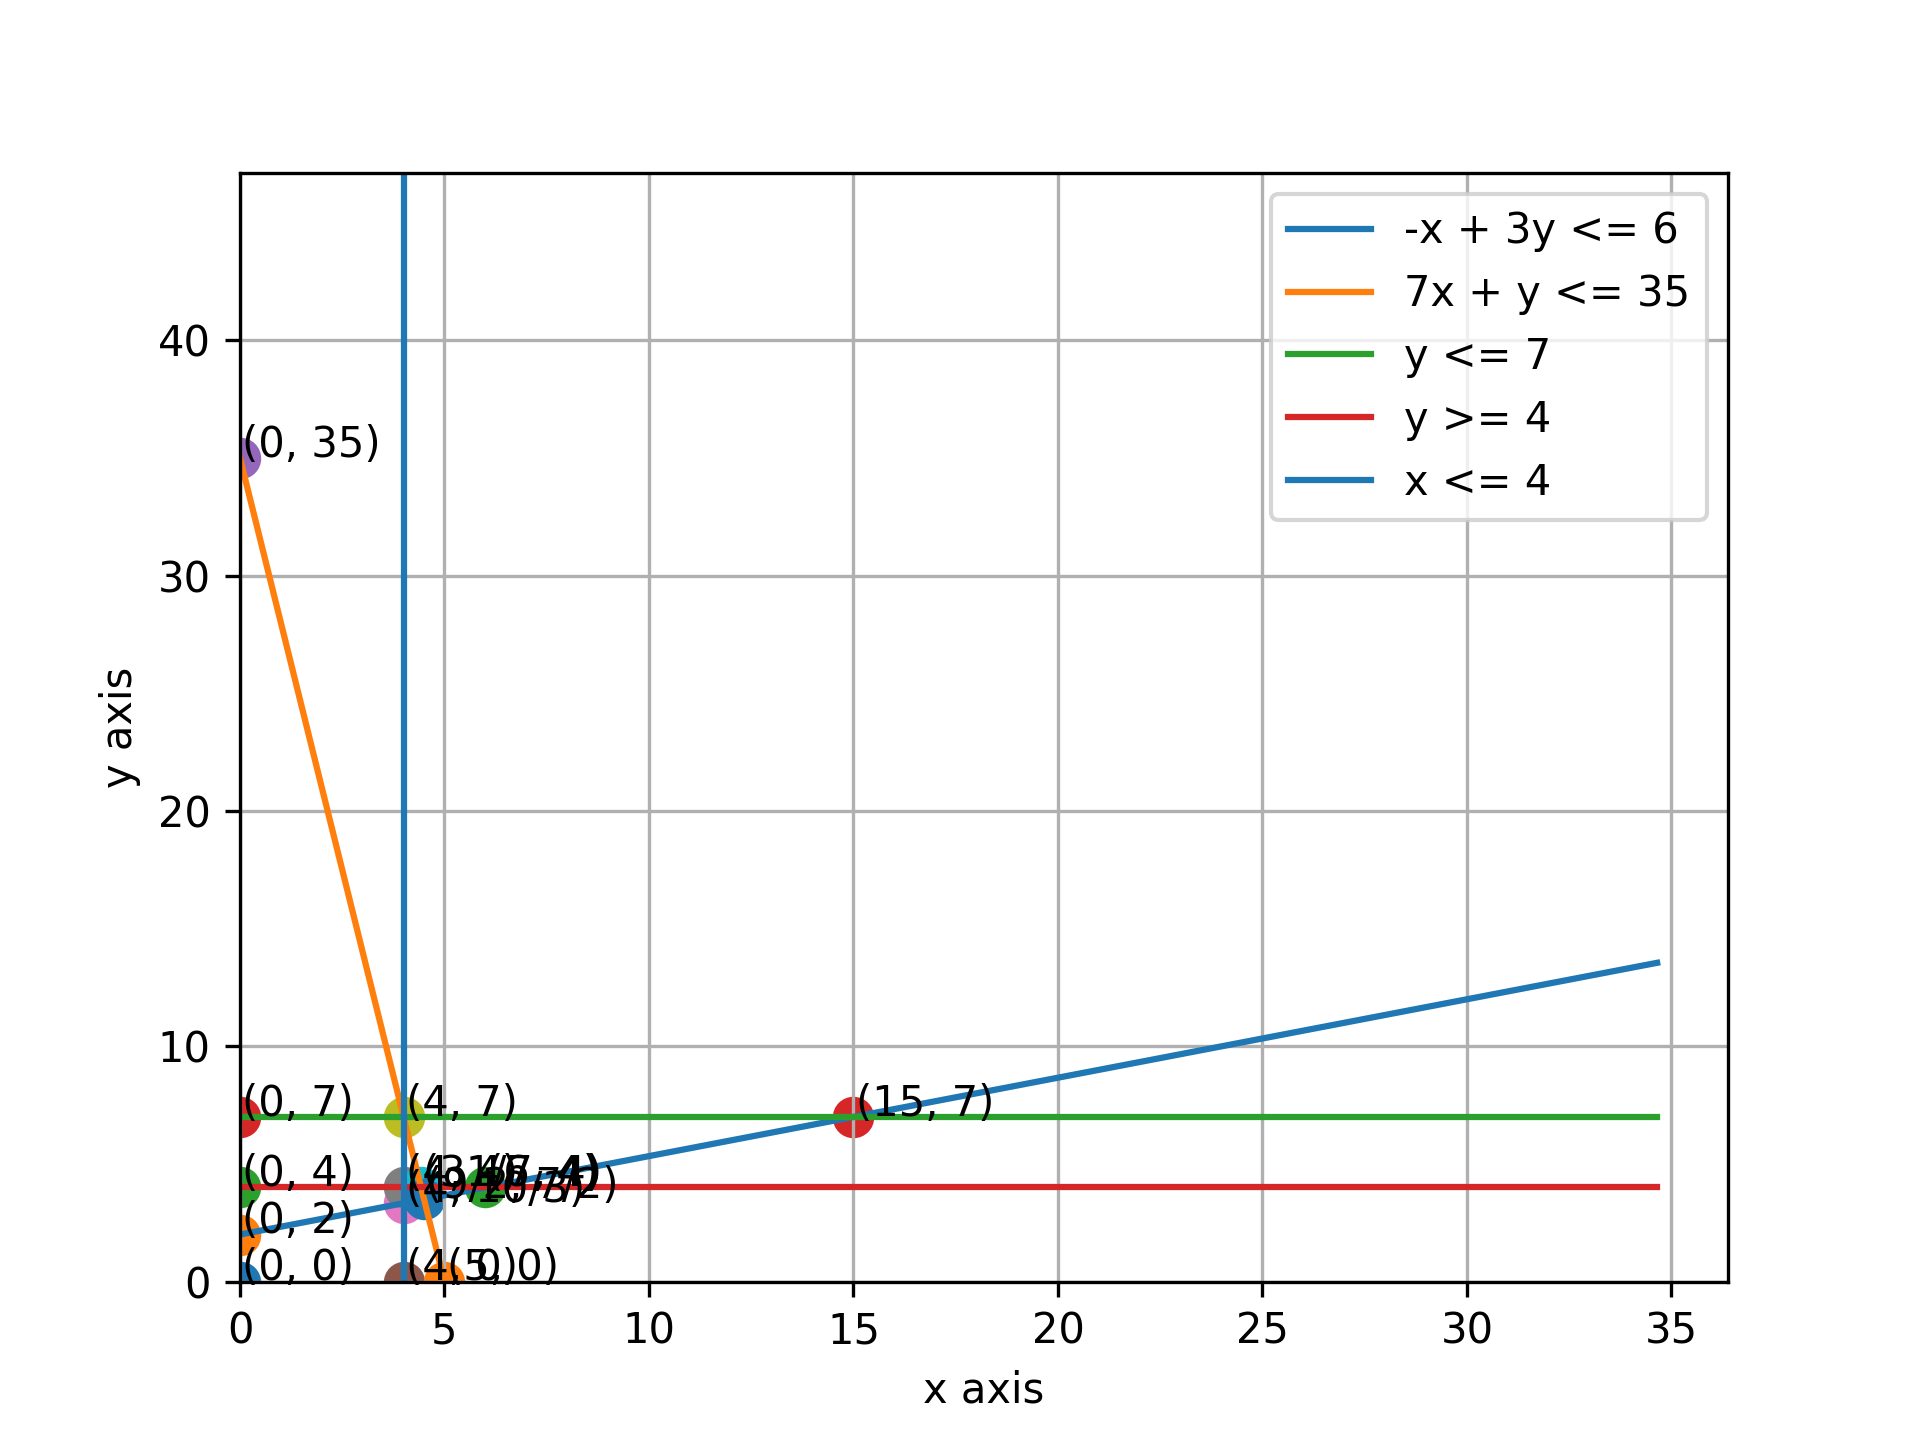
\includegraphics[width=0.6\textwidth]{outputs/ipp2/graph5.png}
\end{center}
Infeasible Solution\\
\begin{align*}
Z=55\end{align*}
\begin{align*}
x=4\end{align*}
\begin{align*}
y=3\end{align*}
\begin{align*}
\text{Maximize} \quad & 2x + 3y\\
\text{subject to} \quad
& 6x + 5y\le12\\
& 4x + 3y\le14\\
& x\ge0,\; y\ge0\end{align*}
\begin{align*}
6x + 5y=12\end{align*}
\begin{align*}
4x + 3y=14\end{align*}
Gauss Elimination:\\
Echelon Form:\\
\begin{align*}
\left(
\begin{array}{cc|c}
6 & 5 & 12\\
4 & 3 & 14\\
\end{array}
\right)_{2\times 3}
\end{align*}
\begin{align*}
\left(
\begin{array}{cc|c}
6 & 5 & 12\\
0 & -\frac{1}{3} & 6\\
\end{array}
\right)_{2\times 3}
\end{align*}
\begin{align*}
\left(
\begin{array}{cc|c}
6 & 5 & 12\\
0 & -\frac{1}{3} & 6\\
\end{array}
\right)_{2\times 3}
\end{align*}
\begin{align*}
x=17\end{align*}
\begin{align*}
y=-18\end{align*}
\begin{center}
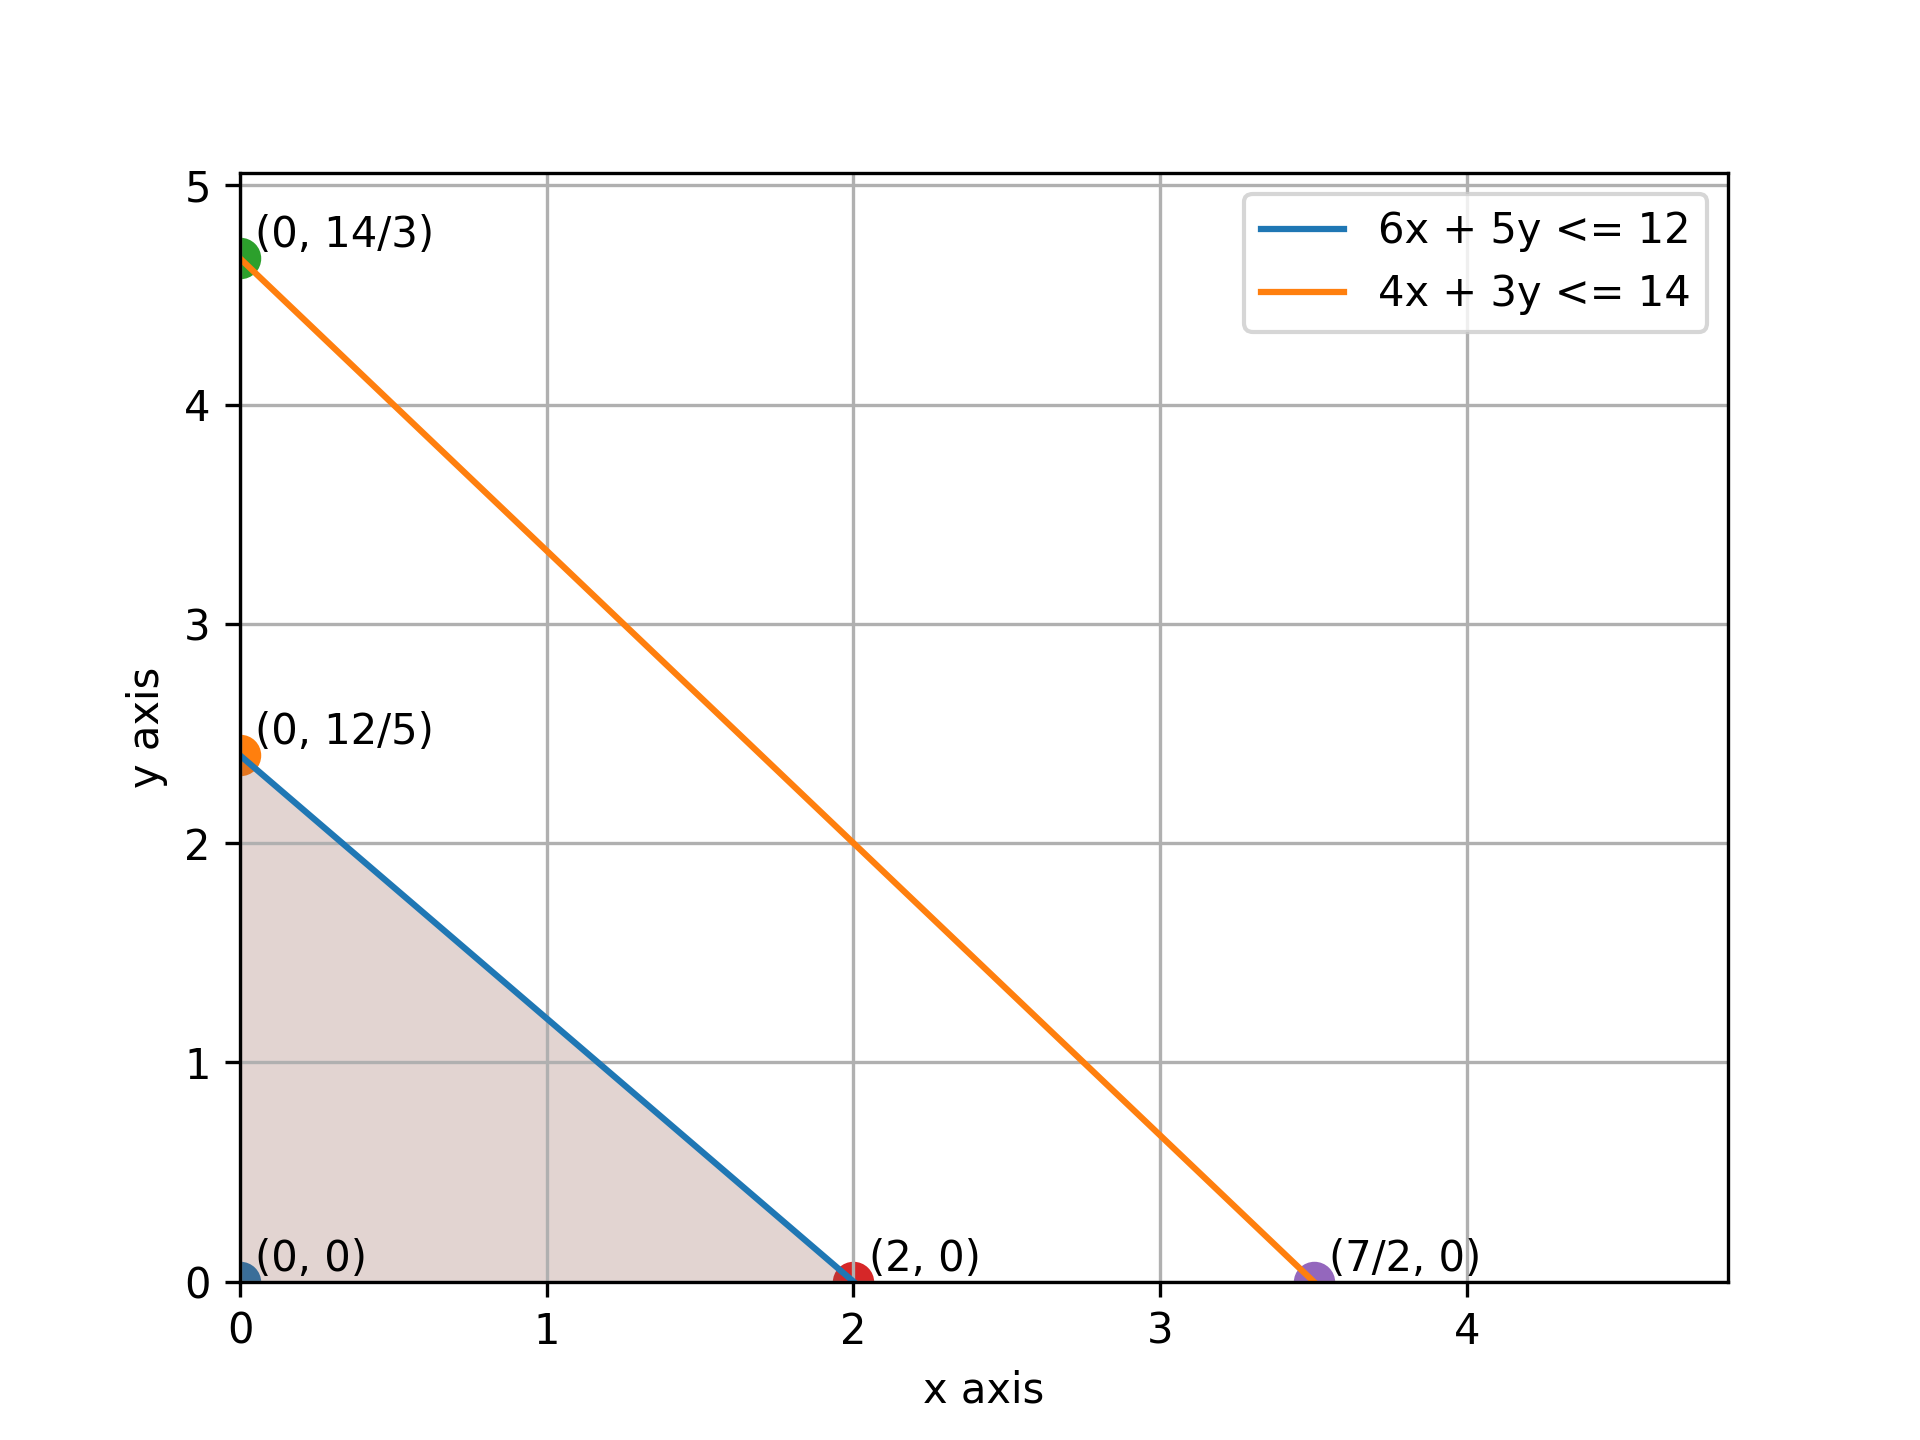
\includegraphics[width=0.6\textwidth]{outputs/ipp3/graph1.png}
\end{center}
\begin{align*}
Z=36\end{align*}
\begin{align*}
x=0\end{align*}
\begin{align*}
y=12\end{align*}
\begin{align*}
\text{Maximize} \quad & 2x + 3y\\
\text{subject to} \quad
& 6x + 5y\le12\\
& 4x + 3y\le14\\
& y\le2\\
& x\ge0,\; y\ge0\end{align*}
\begin{align*}
6x + 5y=12\end{align*}
\begin{align*}
4x + 3y=14\end{align*}
Gauss Elimination:\\
Echelon Form:\\
\begin{align*}
\left(
\begin{array}{cc|c}
6 & 5 & 12\\
4 & 3 & 14\\
\end{array}
\right)_{2\times 3}
\end{align*}
\begin{align*}
\left(
\begin{array}{cc|c}
6 & 5 & 12\\
0 & -\frac{1}{3} & 6\\
\end{array}
\right)_{2\times 3}
\end{align*}
\begin{align*}
\left(
\begin{array}{cc|c}
6 & 5 & 12\\
0 & -\frac{1}{3} & 6\\
\end{array}
\right)_{2\times 3}
\end{align*}
\begin{align*}
x=17\end{align*}
\begin{align*}
y=-18\end{align*}
\begin{align*}
6x + 5y=12\end{align*}
\begin{align*}
y=2\end{align*}
Gauss Elimination:\\
Echelon Form:\\
\begin{align*}
\left(
\begin{array}{cc|c}
6 & 5 & 12\\
0 & 1 & 2\\
\end{array}
\right)_{2\times 3}
\end{align*}
\begin{align*}
\left(
\begin{array}{cc|c}
6 & 5 & 12\\
0 & 1 & 2\\
\end{array}
\right)_{2\times 3}
\end{align*}
\begin{align*}
\left(
\begin{array}{cc|c}
6 & 5 & 12\\
0 & 1 & 2\\
\end{array}
\right)_{2\times 3}
\end{align*}
\begin{align*}
x=\frac{1}{3}\end{align*}
\begin{align*}
y=2\end{align*}
\begin{align*}
4x + 3y=14\end{align*}
\begin{align*}
y=2\end{align*}
Gauss Elimination:\\
Echelon Form:\\
\begin{align*}
\left(
\begin{array}{cc|c}
4 & 3 & 14\\
0 & 1 & 2\\
\end{array}
\right)_{2\times 3}
\end{align*}
\begin{align*}
\left(
\begin{array}{cc|c}
4 & 3 & 14\\
0 & 1 & 2\\
\end{array}
\right)_{2\times 3}
\end{align*}
\begin{align*}
\left(
\begin{array}{cc|c}
4 & 3 & 14\\
0 & 1 & 2\\
\end{array}
\right)_{2\times 3}
\end{align*}
\begin{align*}
x=2\end{align*}
\begin{align*}
y=2\end{align*}
\begin{center}
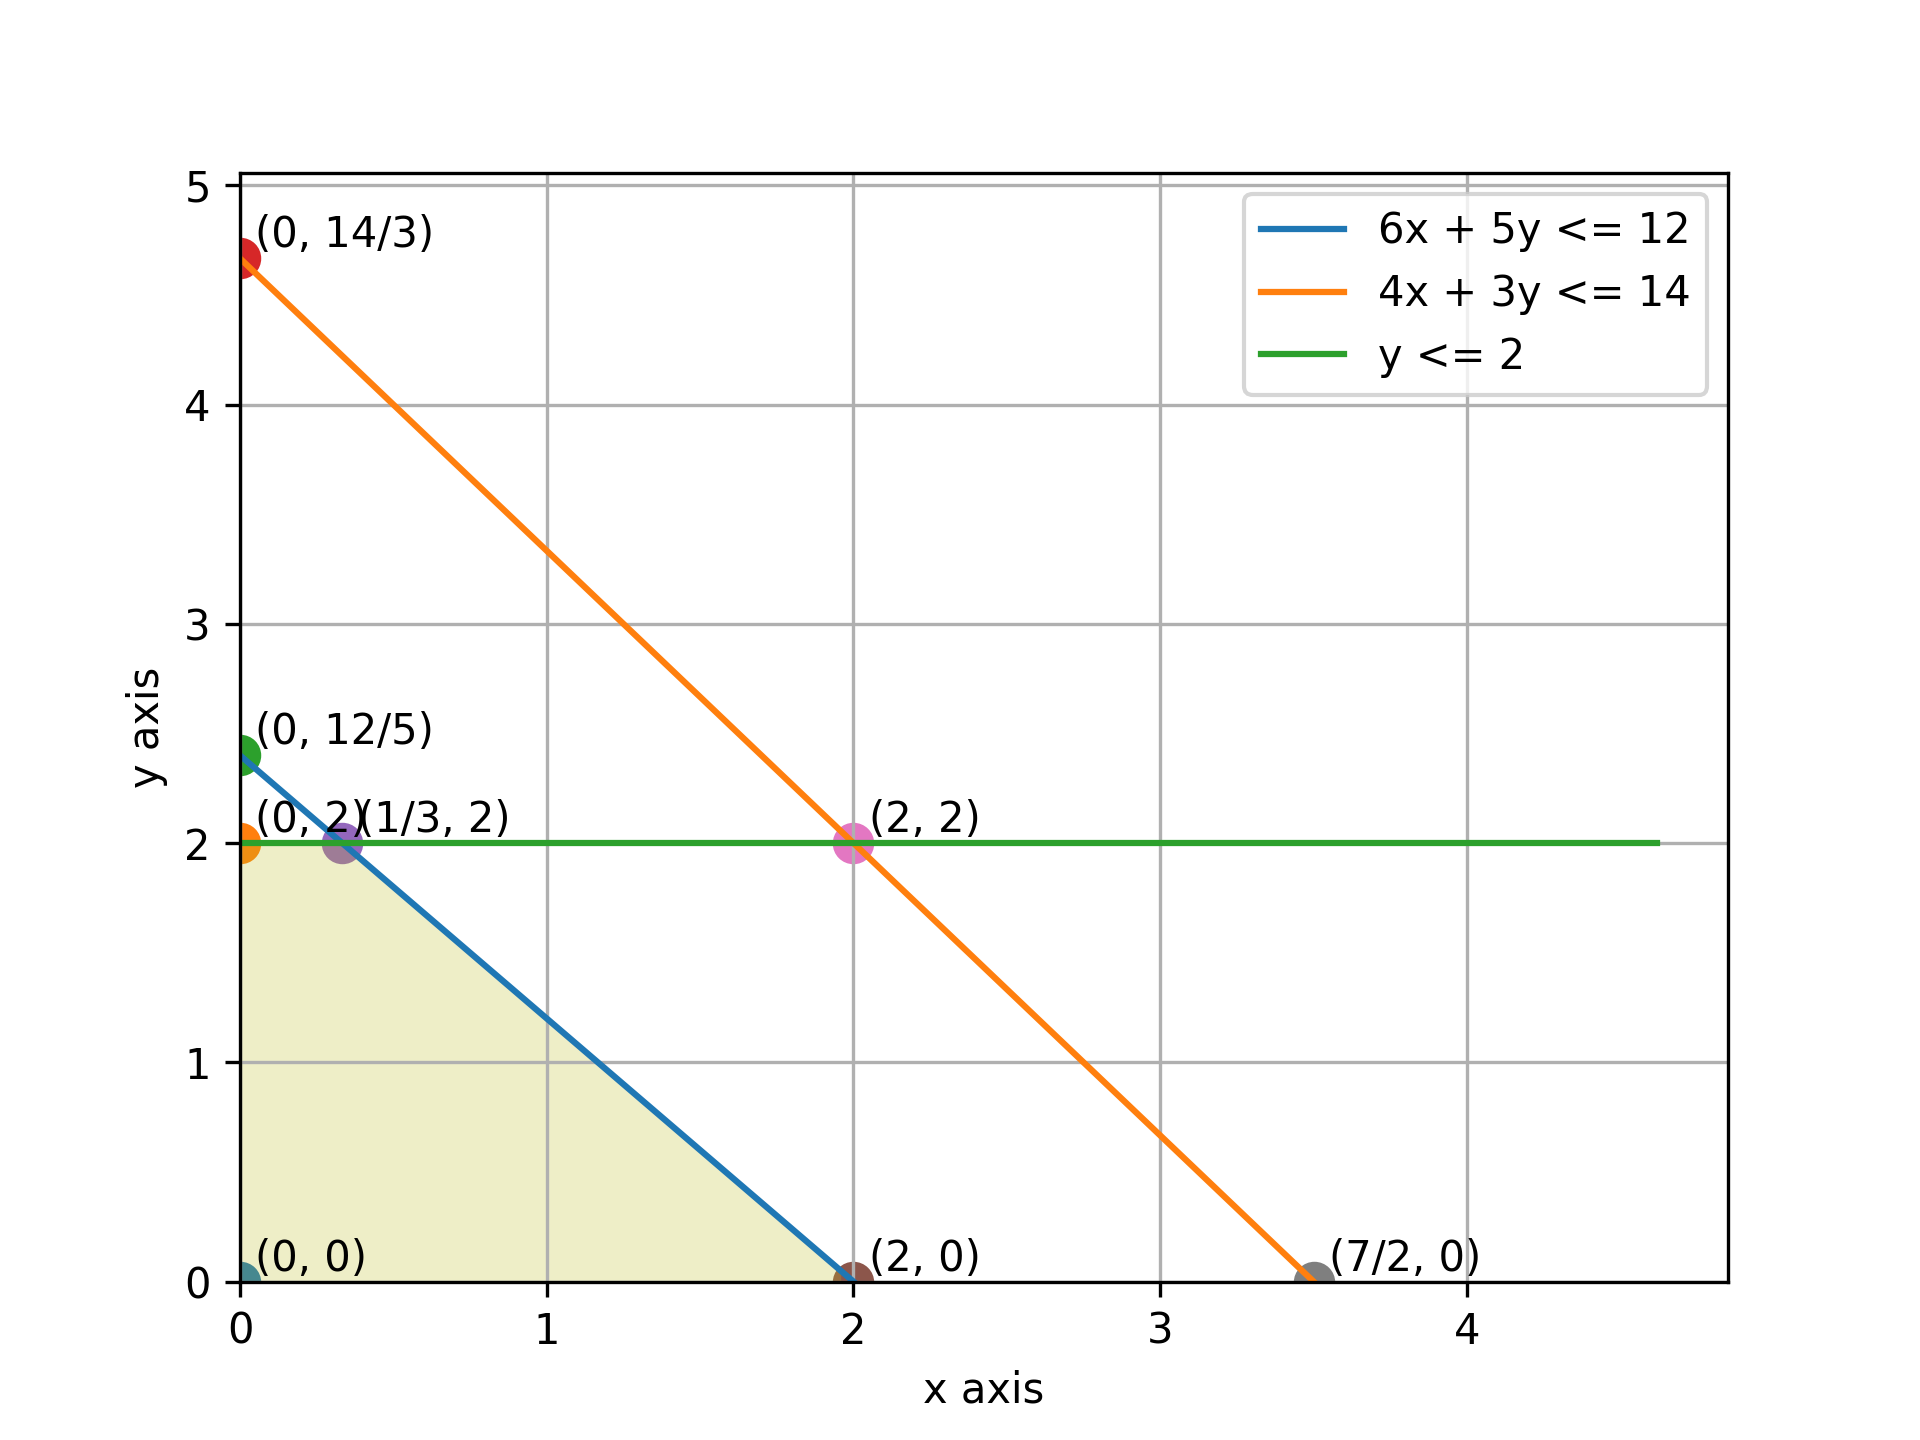
\includegraphics[width=0.6\textwidth]{outputs/ipp3/graph2.png}
\end{center}
\begin{align*}
Z=20\end{align*}
\begin{align*}
x=1\end{align*}
\begin{align*}
y=2\end{align*}
\begin{align*}
\text{Maximize} \quad & 2x + 3y\\
\text{subject to} \quad
& 6x + 5y\le12\\
& 4x + 3y\le14\\
& y\ge3\\
& x\ge0,\; y\ge0\end{align*}
\begin{align*}
6x + 5y=12\end{align*}
\begin{align*}
4x + 3y=14\end{align*}
Gauss Elimination:\\
Echelon Form:\\
\begin{align*}
\left(
\begin{array}{cc|c}
6 & 5 & 12\\
4 & 3 & 14\\
\end{array}
\right)_{2\times 3}
\end{align*}
\begin{align*}
\left(
\begin{array}{cc|c}
6 & 5 & 12\\
0 & -\frac{1}{3} & 6\\
\end{array}
\right)_{2\times 3}
\end{align*}
\begin{align*}
\left(
\begin{array}{cc|c}
6 & 5 & 12\\
0 & -\frac{1}{3} & 6\\
\end{array}
\right)_{2\times 3}
\end{align*}
\begin{align*}
x=17\end{align*}
\begin{align*}
y=-18\end{align*}
\begin{align*}
6x + 5y=12\end{align*}
\begin{align*}
y=3\end{align*}
Gauss Elimination:\\
Echelon Form:\\
\begin{align*}
\left(
\begin{array}{cc|c}
6 & 5 & 12\\
0 & 1 & 3\\
\end{array}
\right)_{2\times 3}
\end{align*}
\begin{align*}
\left(
\begin{array}{cc|c}
6 & 5 & 12\\
0 & 1 & 3\\
\end{array}
\right)_{2\times 3}
\end{align*}
\begin{align*}
\left(
\begin{array}{cc|c}
6 & 5 & 12\\
0 & 1 & 3\\
\end{array}
\right)_{2\times 3}
\end{align*}
\begin{align*}
x=-\frac{1}{2}\end{align*}
\begin{align*}
y=3\end{align*}
\begin{align*}
4x + 3y=14\end{align*}
\begin{align*}
y=3\end{align*}
Gauss Elimination:\\
Echelon Form:\\
\begin{align*}
\left(
\begin{array}{cc|c}
4 & 3 & 14\\
0 & 1 & 3\\
\end{array}
\right)_{2\times 3}
\end{align*}
\begin{align*}
\left(
\begin{array}{cc|c}
4 & 3 & 14\\
0 & 1 & 3\\
\end{array}
\right)_{2\times 3}
\end{align*}
\begin{align*}
\left(
\begin{array}{cc|c}
4 & 3 & 14\\
0 & 1 & 3\\
\end{array}
\right)_{2\times 3}
\end{align*}
\begin{align*}
x=\frac{5}{4}\end{align*}
\begin{align*}
y=3\end{align*}
\begin{center}
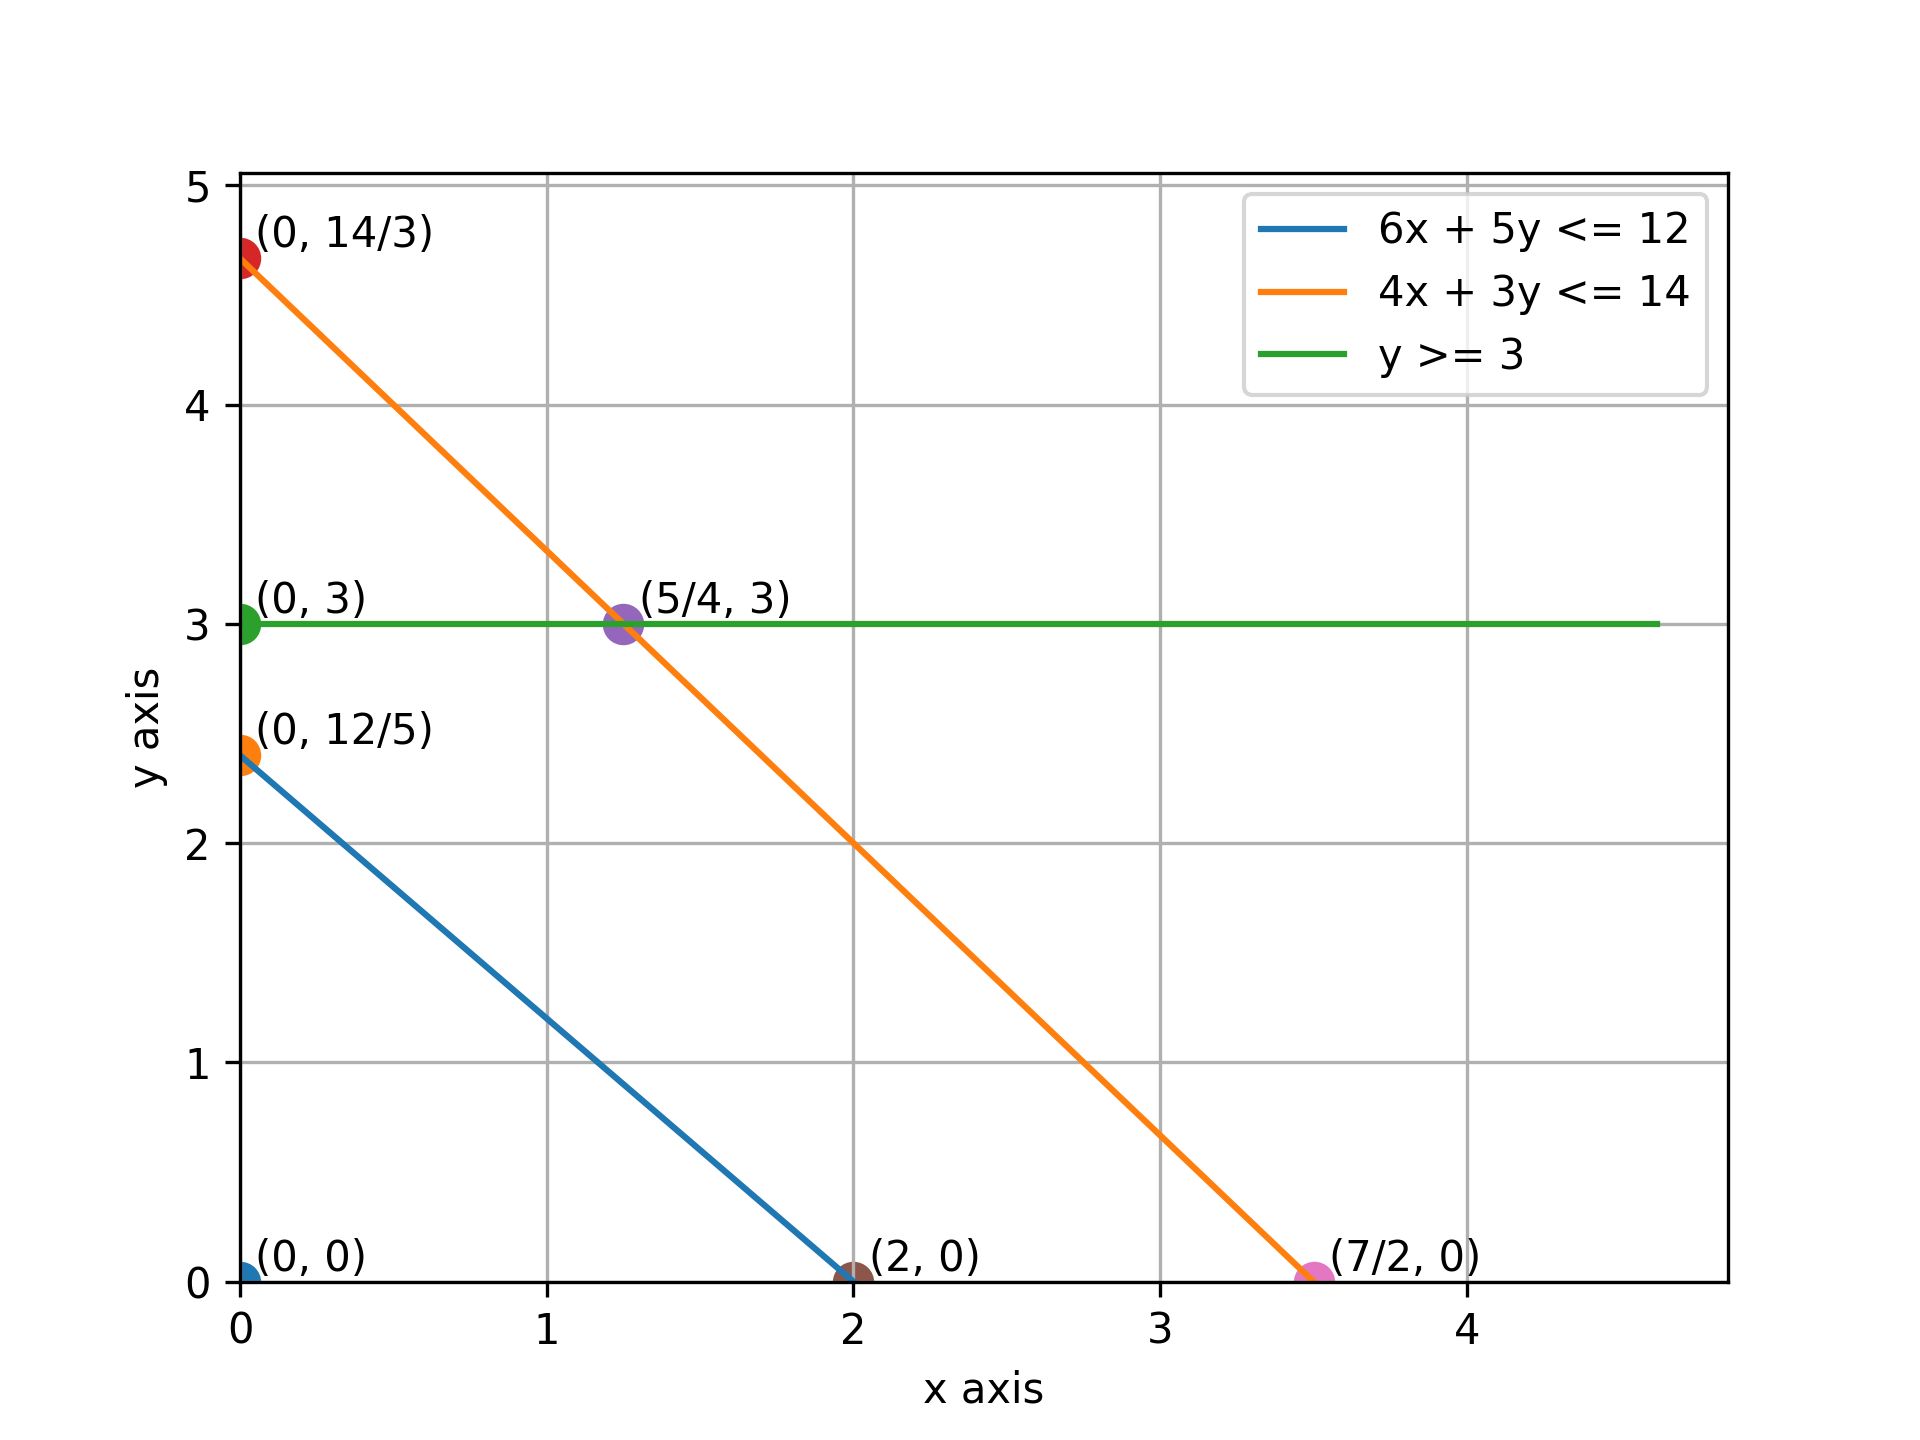
\includegraphics[width=0.6\textwidth]{outputs/ipp3/graph3.png}
\end{center}
Infeasible Solution\\
\begin{align*}
\text{Maximize} \quad & 2x + 3y\\
\text{subject to} \quad
& 6x + 5y\le12\\
& 4x + 3y\le14\\
& y\le2\\
& x\le0\\
& x\ge0,\; y\ge0\end{align*}
\begin{align*}
6x + 5y=12\end{align*}
\begin{align*}
4x + 3y=14\end{align*}
Gauss Elimination:\\
Echelon Form:\\
\begin{align*}
\left(
\begin{array}{cc|c}
6 & 5 & 12\\
4 & 3 & 14\\
\end{array}
\right)_{2\times 3}
\end{align*}
\begin{align*}
\left(
\begin{array}{cc|c}
6 & 5 & 12\\
0 & -\frac{1}{3} & 6\\
\end{array}
\right)_{2\times 3}
\end{align*}
\begin{align*}
\left(
\begin{array}{cc|c}
6 & 5 & 12\\
0 & -\frac{1}{3} & 6\\
\end{array}
\right)_{2\times 3}
\end{align*}
\begin{align*}
x=17\end{align*}
\begin{align*}
y=-18\end{align*}
\begin{align*}
6x + 5y=12\end{align*}
\begin{align*}
y=2\end{align*}
Gauss Elimination:\\
Echelon Form:\\
\begin{align*}
\left(
\begin{array}{cc|c}
6 & 5 & 12\\
0 & 1 & 2\\
\end{array}
\right)_{2\times 3}
\end{align*}
\begin{align*}
\left(
\begin{array}{cc|c}
6 & 5 & 12\\
0 & 1 & 2\\
\end{array}
\right)_{2\times 3}
\end{align*}
\begin{align*}
\left(
\begin{array}{cc|c}
6 & 5 & 12\\
0 & 1 & 2\\
\end{array}
\right)_{2\times 3}
\end{align*}
\begin{align*}
x=\frac{1}{3}\end{align*}
\begin{align*}
y=2\end{align*}
\begin{align*}
6x + 5y=12\end{align*}
\begin{align*}
x=0\end{align*}
Gauss Elimination:\\
Echelon Form:\\
\begin{align*}
\left(
\begin{array}{cc|c}
6 & 5 & 12\\
1 & 0 & 0\\
\end{array}
\right)_{2\times 3}
\end{align*}
\begin{align*}
\left(
\begin{array}{cc|c}
6 & 5 & 12\\
0 & -\frac{5}{6} & -2\\
\end{array}
\right)_{2\times 3}
\end{align*}
\begin{align*}
\left(
\begin{array}{cc|c}
6 & 5 & 12\\
0 & -\frac{5}{6} & -2\\
\end{array}
\right)_{2\times 3}
\end{align*}
\begin{align*}
x=0\end{align*}
\begin{align*}
y=\frac{12}{5}\end{align*}
\begin{align*}
4x + 3y=14\end{align*}
\begin{align*}
y=2\end{align*}
Gauss Elimination:\\
Echelon Form:\\
\begin{align*}
\left(
\begin{array}{cc|c}
4 & 3 & 14\\
0 & 1 & 2\\
\end{array}
\right)_{2\times 3}
\end{align*}
\begin{align*}
\left(
\begin{array}{cc|c}
4 & 3 & 14\\
0 & 1 & 2\\
\end{array}
\right)_{2\times 3}
\end{align*}
\begin{align*}
\left(
\begin{array}{cc|c}
4 & 3 & 14\\
0 & 1 & 2\\
\end{array}
\right)_{2\times 3}
\end{align*}
\begin{align*}
x=2\end{align*}
\begin{align*}
y=2\end{align*}
\begin{align*}
4x + 3y=14\end{align*}
\begin{align*}
x=0\end{align*}
Gauss Elimination:\\
Echelon Form:\\
\begin{align*}
\left(
\begin{array}{cc|c}
4 & 3 & 14\\
1 & 0 & 0\\
\end{array}
\right)_{2\times 3}
\end{align*}
\begin{align*}
\left(
\begin{array}{cc|c}
4 & 3 & 14\\
0 & -\frac{3}{4} & -\frac{7}{2}\\
\end{array}
\right)_{2\times 3}
\end{align*}
\begin{align*}
\left(
\begin{array}{cc|c}
4 & 3 & 14\\
0 & -\frac{3}{4} & -\frac{7}{2}\\
\end{array}
\right)_{2\times 3}
\end{align*}
\begin{align*}
x=0\end{align*}
\begin{align*}
y=\frac{14}{3}\end{align*}
\begin{align*}
y=2\end{align*}
\begin{align*}
x=0\end{align*}
Gauss Elimination:\\
Echelon Form:\\
\begin{align*}
\left(
\begin{array}{cc|c}
0 & 1 & 2\\
1 & 0 & 0\\
\end{array}
\right)_{2\times 3}
\end{align*}
\begin{align*}
\left(
\begin{array}{cc|c}
1 & 0 & 0\\
0 & 1 & 2\\
\end{array}
\right)_{2\times 3}
\end{align*}
\begin{align*}
\left(
\begin{array}{cc|c}
1 & 0 & 0\\
0 & 1 & 2\\
\end{array}
\right)_{2\times 3}
\end{align*}
\begin{align*}
x=0\end{align*}
\begin{align*}
y=2\end{align*}
\begin{center}
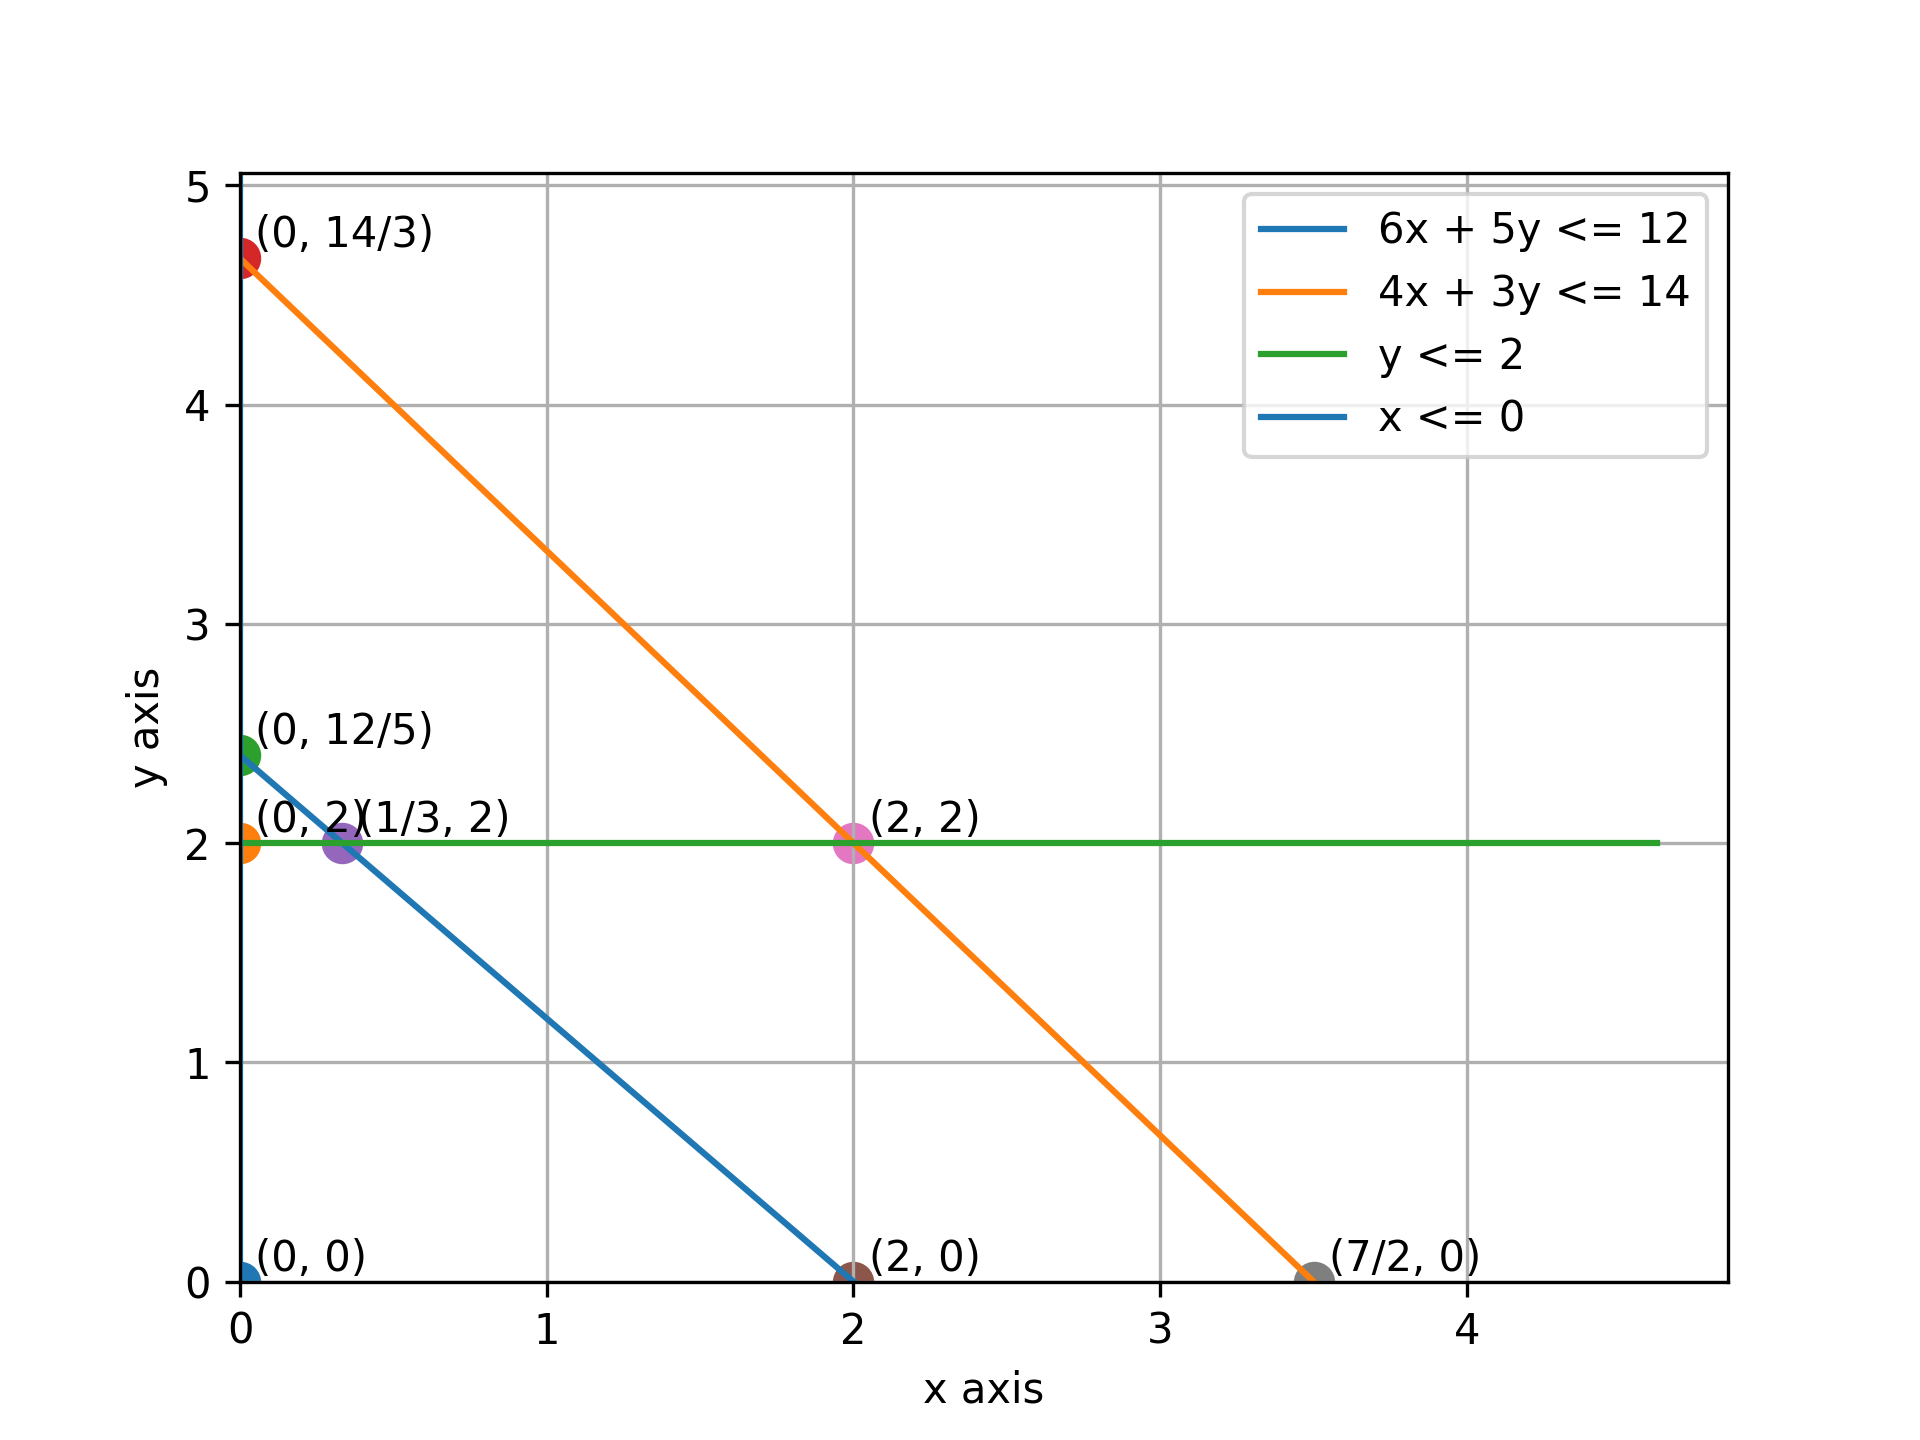
\includegraphics[width=0.6\textwidth]{outputs/ipp3/graph4.png}
\end{center}
\begin{align*}
Z=6\end{align*}
\begin{align*}
x=0\end{align*}
\begin{align*}
y=2\end{align*}
\begin{align*}
\text{Maximize} \quad & 2x + 3y\\
\text{subject to} \quad
& 6x + 5y\le12\\
& 4x + 3y\le14\\
& y\le2\\
& x\ge1\\
& x\ge0,\; y\ge0\end{align*}
\begin{align*}
6x + 5y=12\end{align*}
\begin{align*}
4x + 3y=14\end{align*}
Gauss Elimination:\\
Echelon Form:\\
\begin{align*}
\left(
\begin{array}{cc|c}
6 & 5 & 12\\
4 & 3 & 14\\
\end{array}
\right)_{2\times 3}
\end{align*}
\begin{align*}
\left(
\begin{array}{cc|c}
6 & 5 & 12\\
0 & -\frac{1}{3} & 6\\
\end{array}
\right)_{2\times 3}
\end{align*}
\begin{align*}
\left(
\begin{array}{cc|c}
6 & 5 & 12\\
0 & -\frac{1}{3} & 6\\
\end{array}
\right)_{2\times 3}
\end{align*}
\begin{align*}
x=17\end{align*}
\begin{align*}
y=-18\end{align*}
\begin{align*}
6x + 5y=12\end{align*}
\begin{align*}
y=2\end{align*}
Gauss Elimination:\\
Echelon Form:\\
\begin{align*}
\left(
\begin{array}{cc|c}
6 & 5 & 12\\
0 & 1 & 2\\
\end{array}
\right)_{2\times 3}
\end{align*}
\begin{align*}
\left(
\begin{array}{cc|c}
6 & 5 & 12\\
0 & 1 & 2\\
\end{array}
\right)_{2\times 3}
\end{align*}
\begin{align*}
\left(
\begin{array}{cc|c}
6 & 5 & 12\\
0 & 1 & 2\\
\end{array}
\right)_{2\times 3}
\end{align*}
\begin{align*}
x=\frac{1}{3}\end{align*}
\begin{align*}
y=2\end{align*}
\begin{align*}
6x + 5y=12\end{align*}
\begin{align*}
x=1\end{align*}
Gauss Elimination:\\
Echelon Form:\\
\begin{align*}
\left(
\begin{array}{cc|c}
6 & 5 & 12\\
1 & 0 & 1\\
\end{array}
\right)_{2\times 3}
\end{align*}
\begin{align*}
\left(
\begin{array}{cc|c}
6 & 5 & 12\\
0 & -\frac{5}{6} & -1\\
\end{array}
\right)_{2\times 3}
\end{align*}
\begin{align*}
\left(
\begin{array}{cc|c}
6 & 5 & 12\\
0 & -\frac{5}{6} & -1\\
\end{array}
\right)_{2\times 3}
\end{align*}
\begin{align*}
x=1\end{align*}
\begin{align*}
y=\frac{6}{5}\end{align*}
\begin{align*}
4x + 3y=14\end{align*}
\begin{align*}
y=2\end{align*}
Gauss Elimination:\\
Echelon Form:\\
\begin{align*}
\left(
\begin{array}{cc|c}
4 & 3 & 14\\
0 & 1 & 2\\
\end{array}
\right)_{2\times 3}
\end{align*}
\begin{align*}
\left(
\begin{array}{cc|c}
4 & 3 & 14\\
0 & 1 & 2\\
\end{array}
\right)_{2\times 3}
\end{align*}
\begin{align*}
\left(
\begin{array}{cc|c}
4 & 3 & 14\\
0 & 1 & 2\\
\end{array}
\right)_{2\times 3}
\end{align*}
\begin{align*}
x=2\end{align*}
\begin{align*}
y=2\end{align*}
\begin{align*}
4x + 3y=14\end{align*}
\begin{align*}
x=1\end{align*}
Gauss Elimination:\\
Echelon Form:\\
\begin{align*}
\left(
\begin{array}{cc|c}
4 & 3 & 14\\
1 & 0 & 1\\
\end{array}
\right)_{2\times 3}
\end{align*}
\begin{align*}
\left(
\begin{array}{cc|c}
4 & 3 & 14\\
0 & -\frac{3}{4} & -\frac{5}{2}\\
\end{array}
\right)_{2\times 3}
\end{align*}
\begin{align*}
\left(
\begin{array}{cc|c}
4 & 3 & 14\\
0 & -\frac{3}{4} & -\frac{5}{2}\\
\end{array}
\right)_{2\times 3}
\end{align*}
\begin{align*}
x=1\end{align*}
\begin{align*}
y=\frac{10}{3}\end{align*}
\begin{align*}
y=2\end{align*}
\begin{align*}
x=1\end{align*}
Gauss Elimination:\\
Echelon Form:\\
\begin{align*}
\left(
\begin{array}{cc|c}
0 & 1 & 2\\
1 & 0 & 1\\
\end{array}
\right)_{2\times 3}
\end{align*}
\begin{align*}
\left(
\begin{array}{cc|c}
1 & 0 & 1\\
0 & 1 & 2\\
\end{array}
\right)_{2\times 3}
\end{align*}
\begin{align*}
\left(
\begin{array}{cc|c}
1 & 0 & 1\\
0 & 1 & 2\\
\end{array}
\right)_{2\times 3}
\end{align*}
\begin{align*}
x=1\end{align*}
\begin{align*}
y=2\end{align*}
\begin{center}
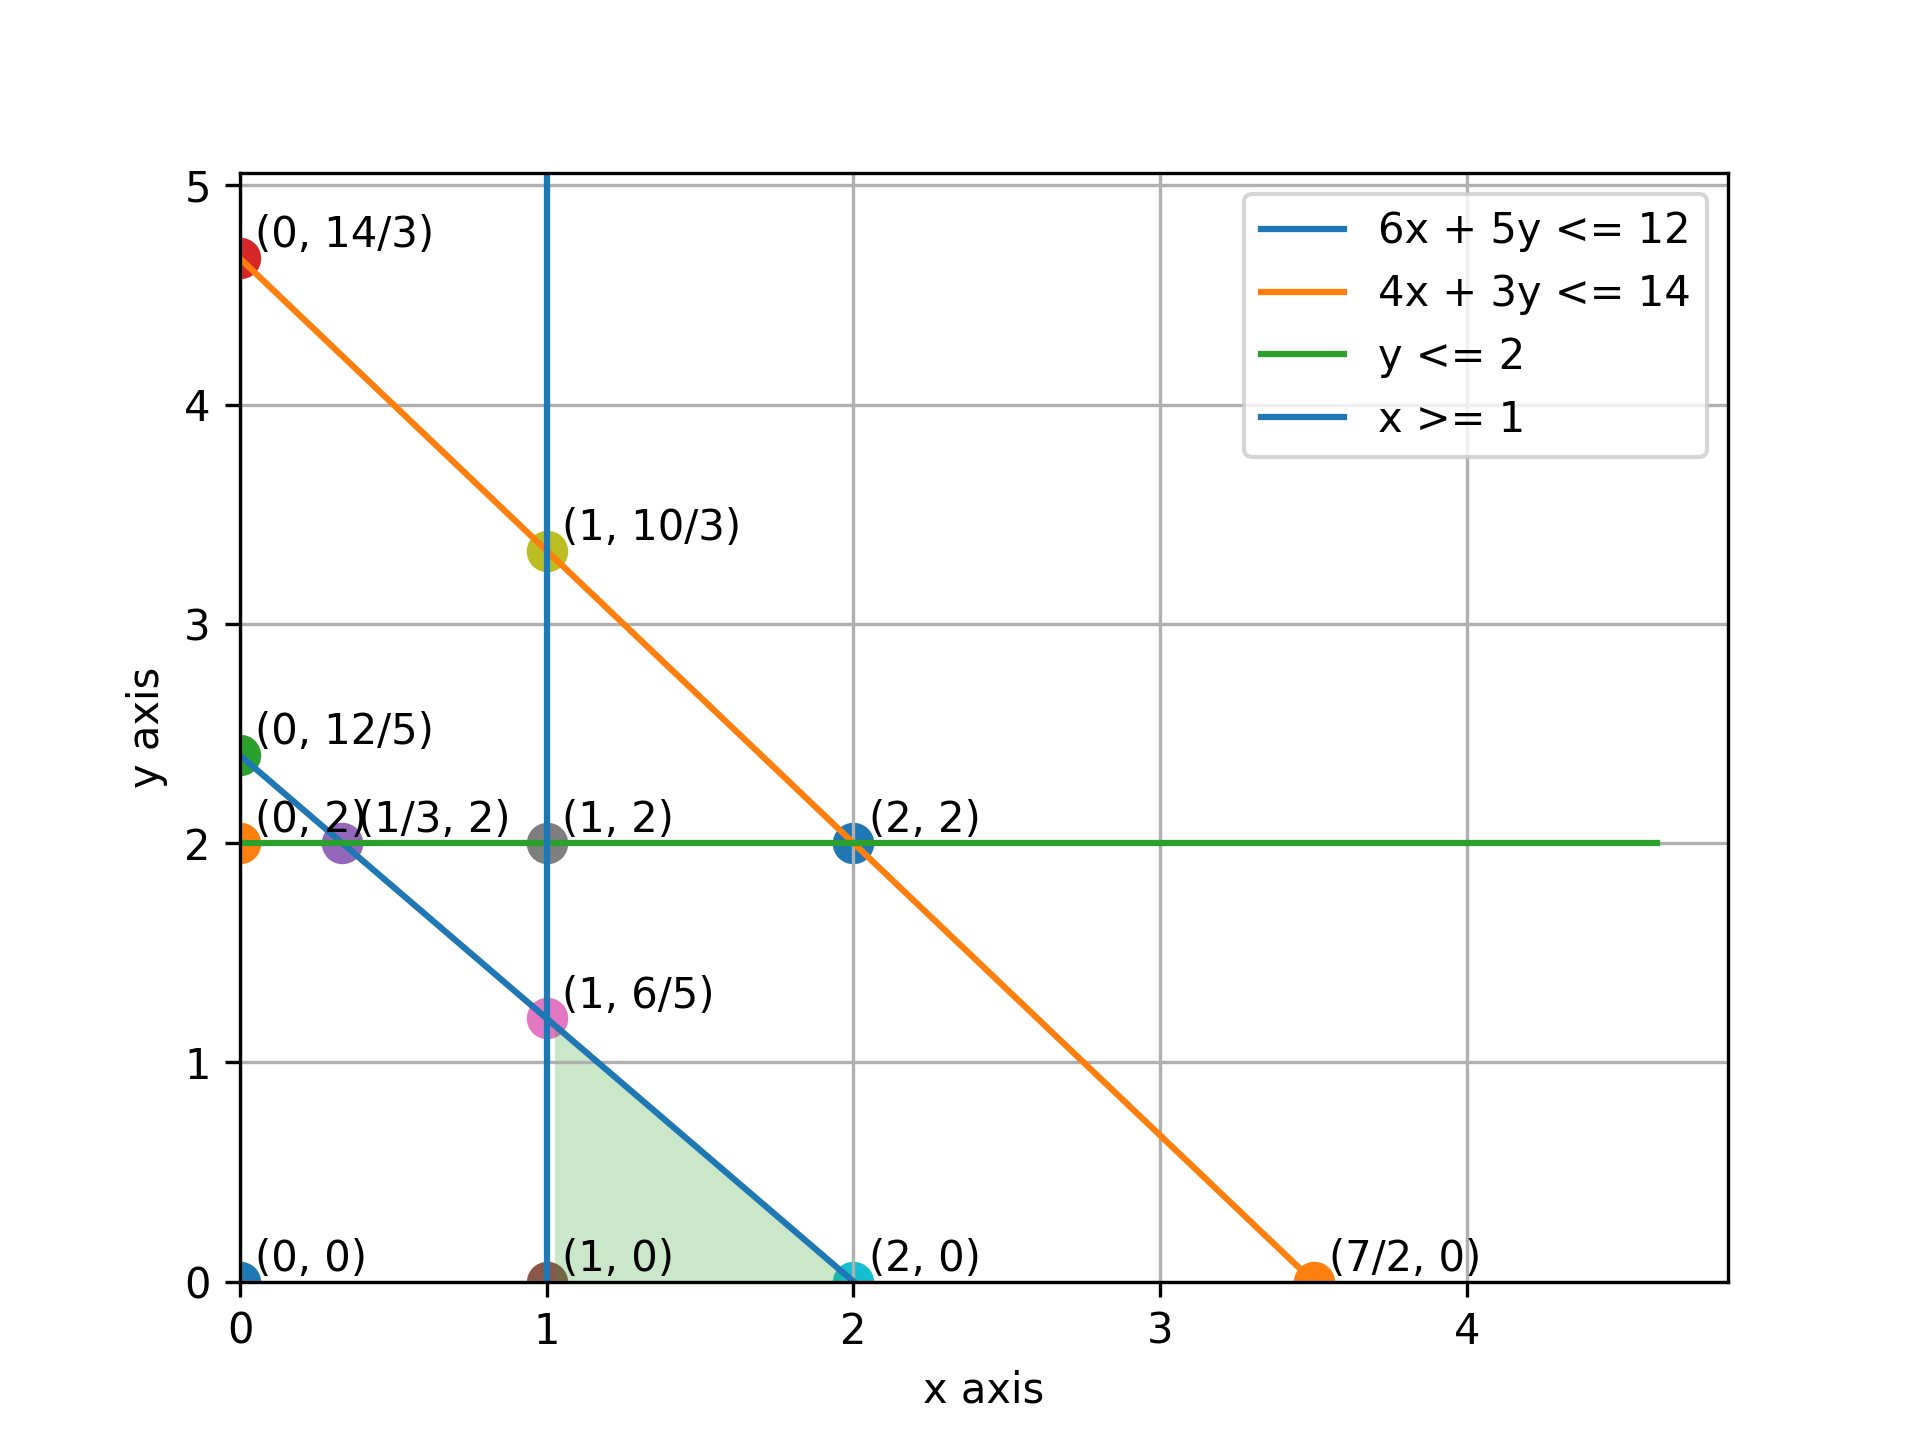
\includegraphics[width=0.6\textwidth]{outputs/ipp3/graph5.png}
\end{center}
\begin{align*}
Z=28\end{align*}
\begin{align*}
x=1\end{align*}
\begin{align*}
y=6\end{align*}
\begin{align*}
\text{Maximize} \quad & 2x + 3y\\
\text{subject to} \quad
& 6x + 5y\le12\\
& 4x + 3y\le14\\
& y\le2\\
& x\ge1\\
& y\le1\\
& x\ge0,\; y\ge0\end{align*}
\begin{align*}
6x + 5y=12\end{align*}
\begin{align*}
4x + 3y=14\end{align*}
Gauss Elimination:\\
Echelon Form:\\
\begin{align*}
\left(
\begin{array}{cc|c}
6 & 5 & 12\\
4 & 3 & 14\\
\end{array}
\right)_{2\times 3}
\end{align*}
\begin{align*}
\left(
\begin{array}{cc|c}
6 & 5 & 12\\
0 & -\frac{1}{3} & 6\\
\end{array}
\right)_{2\times 3}
\end{align*}
\begin{align*}
\left(
\begin{array}{cc|c}
6 & 5 & 12\\
0 & -\frac{1}{3} & 6\\
\end{array}
\right)_{2\times 3}
\end{align*}
\begin{align*}
x=17\end{align*}
\begin{align*}
y=-18\end{align*}
\begin{align*}
6x + 5y=12\end{align*}
\begin{align*}
y=2\end{align*}
Gauss Elimination:\\
Echelon Form:\\
\begin{align*}
\left(
\begin{array}{cc|c}
6 & 5 & 12\\
0 & 1 & 2\\
\end{array}
\right)_{2\times 3}
\end{align*}
\begin{align*}
\left(
\begin{array}{cc|c}
6 & 5 & 12\\
0 & 1 & 2\\
\end{array}
\right)_{2\times 3}
\end{align*}
\begin{align*}
\left(
\begin{array}{cc|c}
6 & 5 & 12\\
0 & 1 & 2\\
\end{array}
\right)_{2\times 3}
\end{align*}
\begin{align*}
x=\frac{1}{3}\end{align*}
\begin{align*}
y=2\end{align*}
\begin{align*}
6x + 5y=12\end{align*}
\begin{align*}
x=1\end{align*}
Gauss Elimination:\\
Echelon Form:\\
\begin{align*}
\left(
\begin{array}{cc|c}
6 & 5 & 12\\
1 & 0 & 1\\
\end{array}
\right)_{2\times 3}
\end{align*}
\begin{align*}
\left(
\begin{array}{cc|c}
6 & 5 & 12\\
0 & -\frac{5}{6} & -1\\
\end{array}
\right)_{2\times 3}
\end{align*}
\begin{align*}
\left(
\begin{array}{cc|c}
6 & 5 & 12\\
0 & -\frac{5}{6} & -1\\
\end{array}
\right)_{2\times 3}
\end{align*}
\begin{align*}
x=1\end{align*}
\begin{align*}
y=\frac{6}{5}\end{align*}
\begin{align*}
6x + 5y=12\end{align*}
\begin{align*}
y=1\end{align*}
Gauss Elimination:\\
Echelon Form:\\
\begin{align*}
\left(
\begin{array}{cc|c}
6 & 5 & 12\\
0 & 1 & 1\\
\end{array}
\right)_{2\times 3}
\end{align*}
\begin{align*}
\left(
\begin{array}{cc|c}
6 & 5 & 12\\
0 & 1 & 1\\
\end{array}
\right)_{2\times 3}
\end{align*}
\begin{align*}
\left(
\begin{array}{cc|c}
6 & 5 & 12\\
0 & 1 & 1\\
\end{array}
\right)_{2\times 3}
\end{align*}
\begin{align*}
x=\frac{7}{6}\end{align*}
\begin{align*}
y=1\end{align*}
\begin{align*}
4x + 3y=14\end{align*}
\begin{align*}
y=2\end{align*}
Gauss Elimination:\\
Echelon Form:\\
\begin{align*}
\left(
\begin{array}{cc|c}
4 & 3 & 14\\
0 & 1 & 2\\
\end{array}
\right)_{2\times 3}
\end{align*}
\begin{align*}
\left(
\begin{array}{cc|c}
4 & 3 & 14\\
0 & 1 & 2\\
\end{array}
\right)_{2\times 3}
\end{align*}
\begin{align*}
\left(
\begin{array}{cc|c}
4 & 3 & 14\\
0 & 1 & 2\\
\end{array}
\right)_{2\times 3}
\end{align*}
\begin{align*}
x=2\end{align*}
\begin{align*}
y=2\end{align*}
\begin{align*}
4x + 3y=14\end{align*}
\begin{align*}
x=1\end{align*}
Gauss Elimination:\\
Echelon Form:\\
\begin{align*}
\left(
\begin{array}{cc|c}
4 & 3 & 14\\
1 & 0 & 1\\
\end{array}
\right)_{2\times 3}
\end{align*}
\begin{align*}
\left(
\begin{array}{cc|c}
4 & 3 & 14\\
0 & -\frac{3}{4} & -\frac{5}{2}\\
\end{array}
\right)_{2\times 3}
\end{align*}
\begin{align*}
\left(
\begin{array}{cc|c}
4 & 3 & 14\\
0 & -\frac{3}{4} & -\frac{5}{2}\\
\end{array}
\right)_{2\times 3}
\end{align*}
\begin{align*}
x=1\end{align*}
\begin{align*}
y=\frac{10}{3}\end{align*}
\begin{align*}
4x + 3y=14\end{align*}
\begin{align*}
y=1\end{align*}
Gauss Elimination:\\
Echelon Form:\\
\begin{align*}
\left(
\begin{array}{cc|c}
4 & 3 & 14\\
0 & 1 & 1\\
\end{array}
\right)_{2\times 3}
\end{align*}
\begin{align*}
\left(
\begin{array}{cc|c}
4 & 3 & 14\\
0 & 1 & 1\\
\end{array}
\right)_{2\times 3}
\end{align*}
\begin{align*}
\left(
\begin{array}{cc|c}
4 & 3 & 14\\
0 & 1 & 1\\
\end{array}
\right)_{2\times 3}
\end{align*}
\begin{align*}
x=\frac{11}{4}\end{align*}
\begin{align*}
y=1\end{align*}
\begin{align*}
y=2\end{align*}
\begin{align*}
x=1\end{align*}
Gauss Elimination:\\
Echelon Form:\\
\begin{align*}
\left(
\begin{array}{cc|c}
0 & 1 & 2\\
1 & 0 & 1\\
\end{array}
\right)_{2\times 3}
\end{align*}
\begin{align*}
\left(
\begin{array}{cc|c}
1 & 0 & 1\\
0 & 1 & 2\\
\end{array}
\right)_{2\times 3}
\end{align*}
\begin{align*}
\left(
\begin{array}{cc|c}
1 & 0 & 1\\
0 & 1 & 2\\
\end{array}
\right)_{2\times 3}
\end{align*}
\begin{align*}
x=1\end{align*}
\begin{align*}
y=2\end{align*}
\begin{align*}
y=2\end{align*}
\begin{align*}
y=1\end{align*}
Gauss Elimination:\\
Echelon Form:\\
\begin{align*}
\left(
\begin{array}{c|c}
1 & 2\\
1 & 1\\
\end{array}
\right)_{2\times 2}
\end{align*}
\begin{align*}
\left(
\begin{array}{c|c}
1 & 2\\
0 & -1\\
\end{array}
\right)_{2\times 2}
\end{align*}
\begin{align*}
\left(
\begin{array}{c|c}
1 & 2\\
0 & -1\\
\end{array}
\right)_{2\times 2}
\end{align*}
No solution\\
\begin{align*}
x=1\end{align*}
\begin{align*}
y=1\end{align*}
Gauss Elimination:\\
Echelon Form:\\
\begin{align*}
\left(
\begin{array}{cc|c}
1 & 0 & 1\\
0 & 1 & 1\\
\end{array}
\right)_{2\times 3}
\end{align*}
\begin{align*}
\left(
\begin{array}{cc|c}
1 & 0 & 1\\
0 & 1 & 1\\
\end{array}
\right)_{2\times 3}
\end{align*}
\begin{align*}
\left(
\begin{array}{cc|c}
1 & 0 & 1\\
0 & 1 & 1\\
\end{array}
\right)_{2\times 3}
\end{align*}
\begin{align*}
x=1\end{align*}
\begin{align*}
y=1\end{align*}
\begin{center}
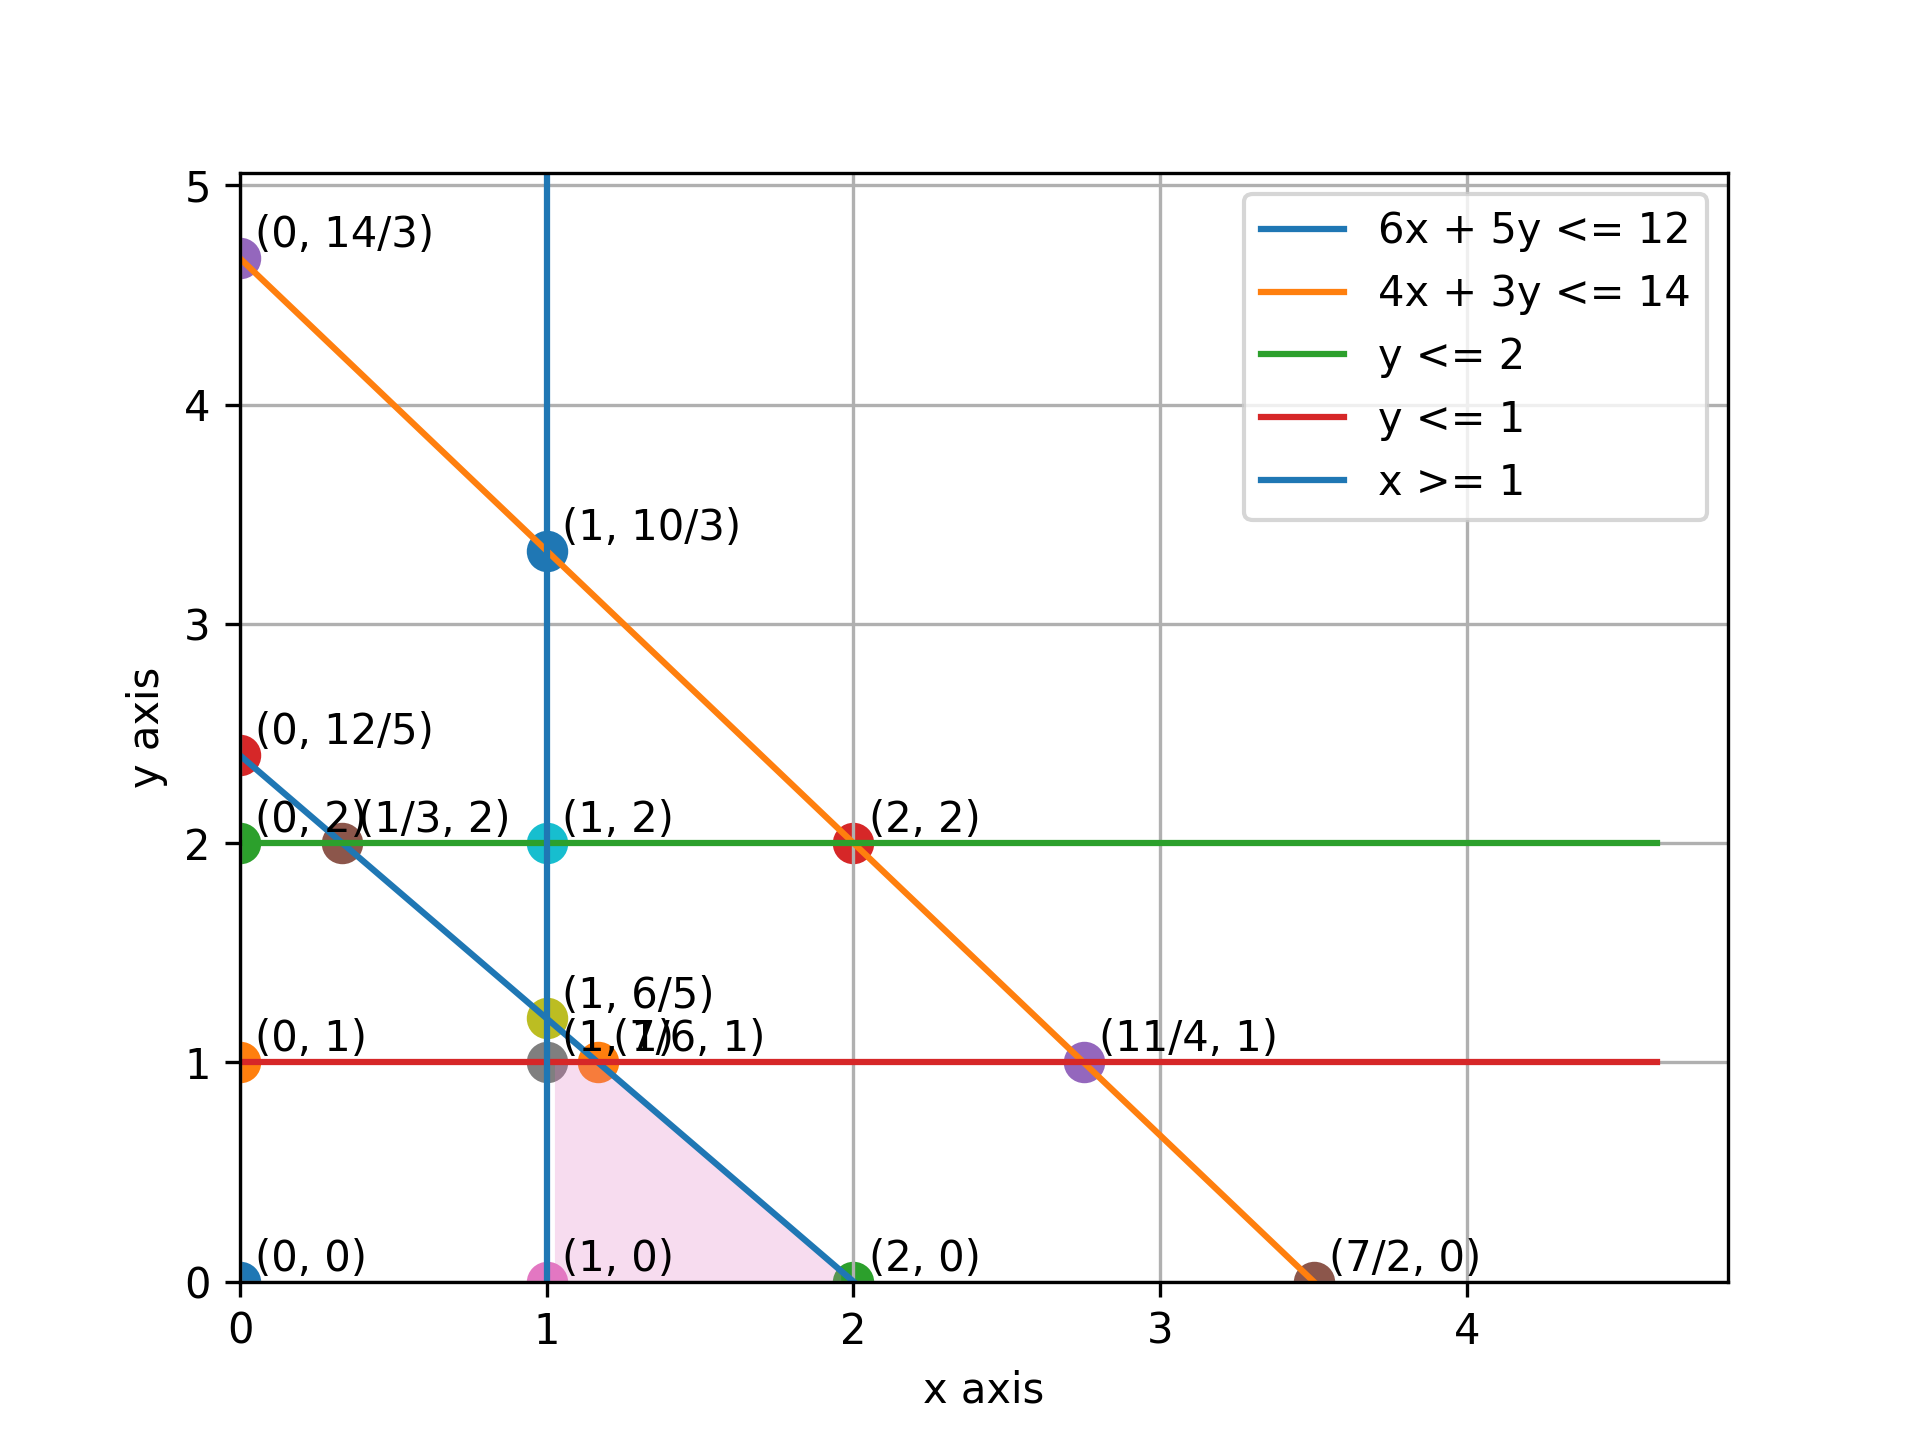
\includegraphics[width=0.6\textwidth]{outputs/ipp3/graph6.png}
\end{center}
\begin{align*}
Z=16\end{align*}
\begin{align*}
x=7\end{align*}
\begin{align*}
y=1\end{align*}
\begin{align*}
\text{Maximize} \quad & 2x + 3y\\
\text{subject to} \quad
& 6x + 5y\le12\\
& 4x + 3y\le14\\
& y\le2\\
& x\ge1\\
& y\ge2\\
& x\ge0,\; y\ge0\end{align*}
\begin{align*}
6x + 5y=12\end{align*}
\begin{align*}
4x + 3y=14\end{align*}
Gauss Elimination:\\
Echelon Form:\\
\begin{align*}
\left(
\begin{array}{cc|c}
6 & 5 & 12\\
4 & 3 & 14\\
\end{array}
\right)_{2\times 3}
\end{align*}
\begin{align*}
\left(
\begin{array}{cc|c}
6 & 5 & 12\\
0 & -\frac{1}{3} & 6\\
\end{array}
\right)_{2\times 3}
\end{align*}
\begin{align*}
\left(
\begin{array}{cc|c}
6 & 5 & 12\\
0 & -\frac{1}{3} & 6\\
\end{array}
\right)_{2\times 3}
\end{align*}
\begin{align*}
x=17\end{align*}
\begin{align*}
y=-18\end{align*}
\begin{align*}
6x + 5y=12\end{align*}
\begin{align*}
y=2\end{align*}
Gauss Elimination:\\
Echelon Form:\\
\begin{align*}
\left(
\begin{array}{cc|c}
6 & 5 & 12\\
0 & 1 & 2\\
\end{array}
\right)_{2\times 3}
\end{align*}
\begin{align*}
\left(
\begin{array}{cc|c}
6 & 5 & 12\\
0 & 1 & 2\\
\end{array}
\right)_{2\times 3}
\end{align*}
\begin{align*}
\left(
\begin{array}{cc|c}
6 & 5 & 12\\
0 & 1 & 2\\
\end{array}
\right)_{2\times 3}
\end{align*}
\begin{align*}
x=\frac{1}{3}\end{align*}
\begin{align*}
y=2\end{align*}
\begin{align*}
6x + 5y=12\end{align*}
\begin{align*}
x=1\end{align*}
Gauss Elimination:\\
Echelon Form:\\
\begin{align*}
\left(
\begin{array}{cc|c}
6 & 5 & 12\\
1 & 0 & 1\\
\end{array}
\right)_{2\times 3}
\end{align*}
\begin{align*}
\left(
\begin{array}{cc|c}
6 & 5 & 12\\
0 & -\frac{5}{6} & -1\\
\end{array}
\right)_{2\times 3}
\end{align*}
\begin{align*}
\left(
\begin{array}{cc|c}
6 & 5 & 12\\
0 & -\frac{5}{6} & -1\\
\end{array}
\right)_{2\times 3}
\end{align*}
\begin{align*}
x=1\end{align*}
\begin{align*}
y=\frac{6}{5}\end{align*}
\begin{align*}
6x + 5y=12\end{align*}
\begin{align*}
y=2\end{align*}
Gauss Elimination:\\
Echelon Form:\\
\begin{align*}
\left(
\begin{array}{cc|c}
6 & 5 & 12\\
0 & 1 & 2\\
\end{array}
\right)_{2\times 3}
\end{align*}
\begin{align*}
\left(
\begin{array}{cc|c}
6 & 5 & 12\\
0 & 1 & 2\\
\end{array}
\right)_{2\times 3}
\end{align*}
\begin{align*}
\left(
\begin{array}{cc|c}
6 & 5 & 12\\
0 & 1 & 2\\
\end{array}
\right)_{2\times 3}
\end{align*}
\begin{align*}
x=\frac{1}{3}\end{align*}
\begin{align*}
y=2\end{align*}
\begin{align*}
4x + 3y=14\end{align*}
\begin{align*}
y=2\end{align*}
Gauss Elimination:\\
Echelon Form:\\
\begin{align*}
\left(
\begin{array}{cc|c}
4 & 3 & 14\\
0 & 1 & 2\\
\end{array}
\right)_{2\times 3}
\end{align*}
\begin{align*}
\left(
\begin{array}{cc|c}
4 & 3 & 14\\
0 & 1 & 2\\
\end{array}
\right)_{2\times 3}
\end{align*}
\begin{align*}
\left(
\begin{array}{cc|c}
4 & 3 & 14\\
0 & 1 & 2\\
\end{array}
\right)_{2\times 3}
\end{align*}
\begin{align*}
x=2\end{align*}
\begin{align*}
y=2\end{align*}
\begin{align*}
4x + 3y=14\end{align*}
\begin{align*}
x=1\end{align*}
Gauss Elimination:\\
Echelon Form:\\
\begin{align*}
\left(
\begin{array}{cc|c}
4 & 3 & 14\\
1 & 0 & 1\\
\end{array}
\right)_{2\times 3}
\end{align*}
\begin{align*}
\left(
\begin{array}{cc|c}
4 & 3 & 14\\
0 & -\frac{3}{4} & -\frac{5}{2}\\
\end{array}
\right)_{2\times 3}
\end{align*}
\begin{align*}
\left(
\begin{array}{cc|c}
4 & 3 & 14\\
0 & -\frac{3}{4} & -\frac{5}{2}\\
\end{array}
\right)_{2\times 3}
\end{align*}
\begin{align*}
x=1\end{align*}
\begin{align*}
y=\frac{10}{3}\end{align*}
\begin{align*}
4x + 3y=14\end{align*}
\begin{align*}
y=2\end{align*}
Gauss Elimination:\\
Echelon Form:\\
\begin{align*}
\left(
\begin{array}{cc|c}
4 & 3 & 14\\
0 & 1 & 2\\
\end{array}
\right)_{2\times 3}
\end{align*}
\begin{align*}
\left(
\begin{array}{cc|c}
4 & 3 & 14\\
0 & 1 & 2\\
\end{array}
\right)_{2\times 3}
\end{align*}
\begin{align*}
\left(
\begin{array}{cc|c}
4 & 3 & 14\\
0 & 1 & 2\\
\end{array}
\right)_{2\times 3}
\end{align*}
\begin{align*}
x=2\end{align*}
\begin{align*}
y=2\end{align*}
\begin{align*}
y=2\end{align*}
\begin{align*}
x=1\end{align*}
Gauss Elimination:\\
Echelon Form:\\
\begin{align*}
\left(
\begin{array}{cc|c}
0 & 1 & 2\\
1 & 0 & 1\\
\end{array}
\right)_{2\times 3}
\end{align*}
\begin{align*}
\left(
\begin{array}{cc|c}
1 & 0 & 1\\
0 & 1 & 2\\
\end{array}
\right)_{2\times 3}
\end{align*}
\begin{align*}
\left(
\begin{array}{cc|c}
1 & 0 & 1\\
0 & 1 & 2\\
\end{array}
\right)_{2\times 3}
\end{align*}
\begin{align*}
x=1\end{align*}
\begin{align*}
y=2\end{align*}
\begin{align*}
y=2\end{align*}
\begin{align*}
y=2\end{align*}
Gauss Elimination:\\
Echelon Form:\\
\begin{align*}
\left(
\begin{array}{c|c}
1 & 2\\
1 & 2\\
\end{array}
\right)_{2\times 2}
\end{align*}
\begin{align*}
\left(
\begin{array}{c|c}
1 & 2\\
0 & 0\\
\end{array}
\right)_{2\times 2}
\end{align*}
Infinitely many solutions\\
\begin{align*}
x=1\end{align*}
\begin{align*}
y=2\end{align*}
Gauss Elimination:\\
Echelon Form:\\
\begin{align*}
\left(
\begin{array}{cc|c}
1 & 0 & 1\\
0 & 1 & 2\\
\end{array}
\right)_{2\times 3}
\end{align*}
\begin{align*}
\left(
\begin{array}{cc|c}
1 & 0 & 1\\
0 & 1 & 2\\
\end{array}
\right)_{2\times 3}
\end{align*}
\begin{align*}
\left(
\begin{array}{cc|c}
1 & 0 & 1\\
0 & 1 & 2\\
\end{array}
\right)_{2\times 3}
\end{align*}
\begin{align*}
x=1\end{align*}
\begin{align*}
y=2\end{align*}
\begin{center}
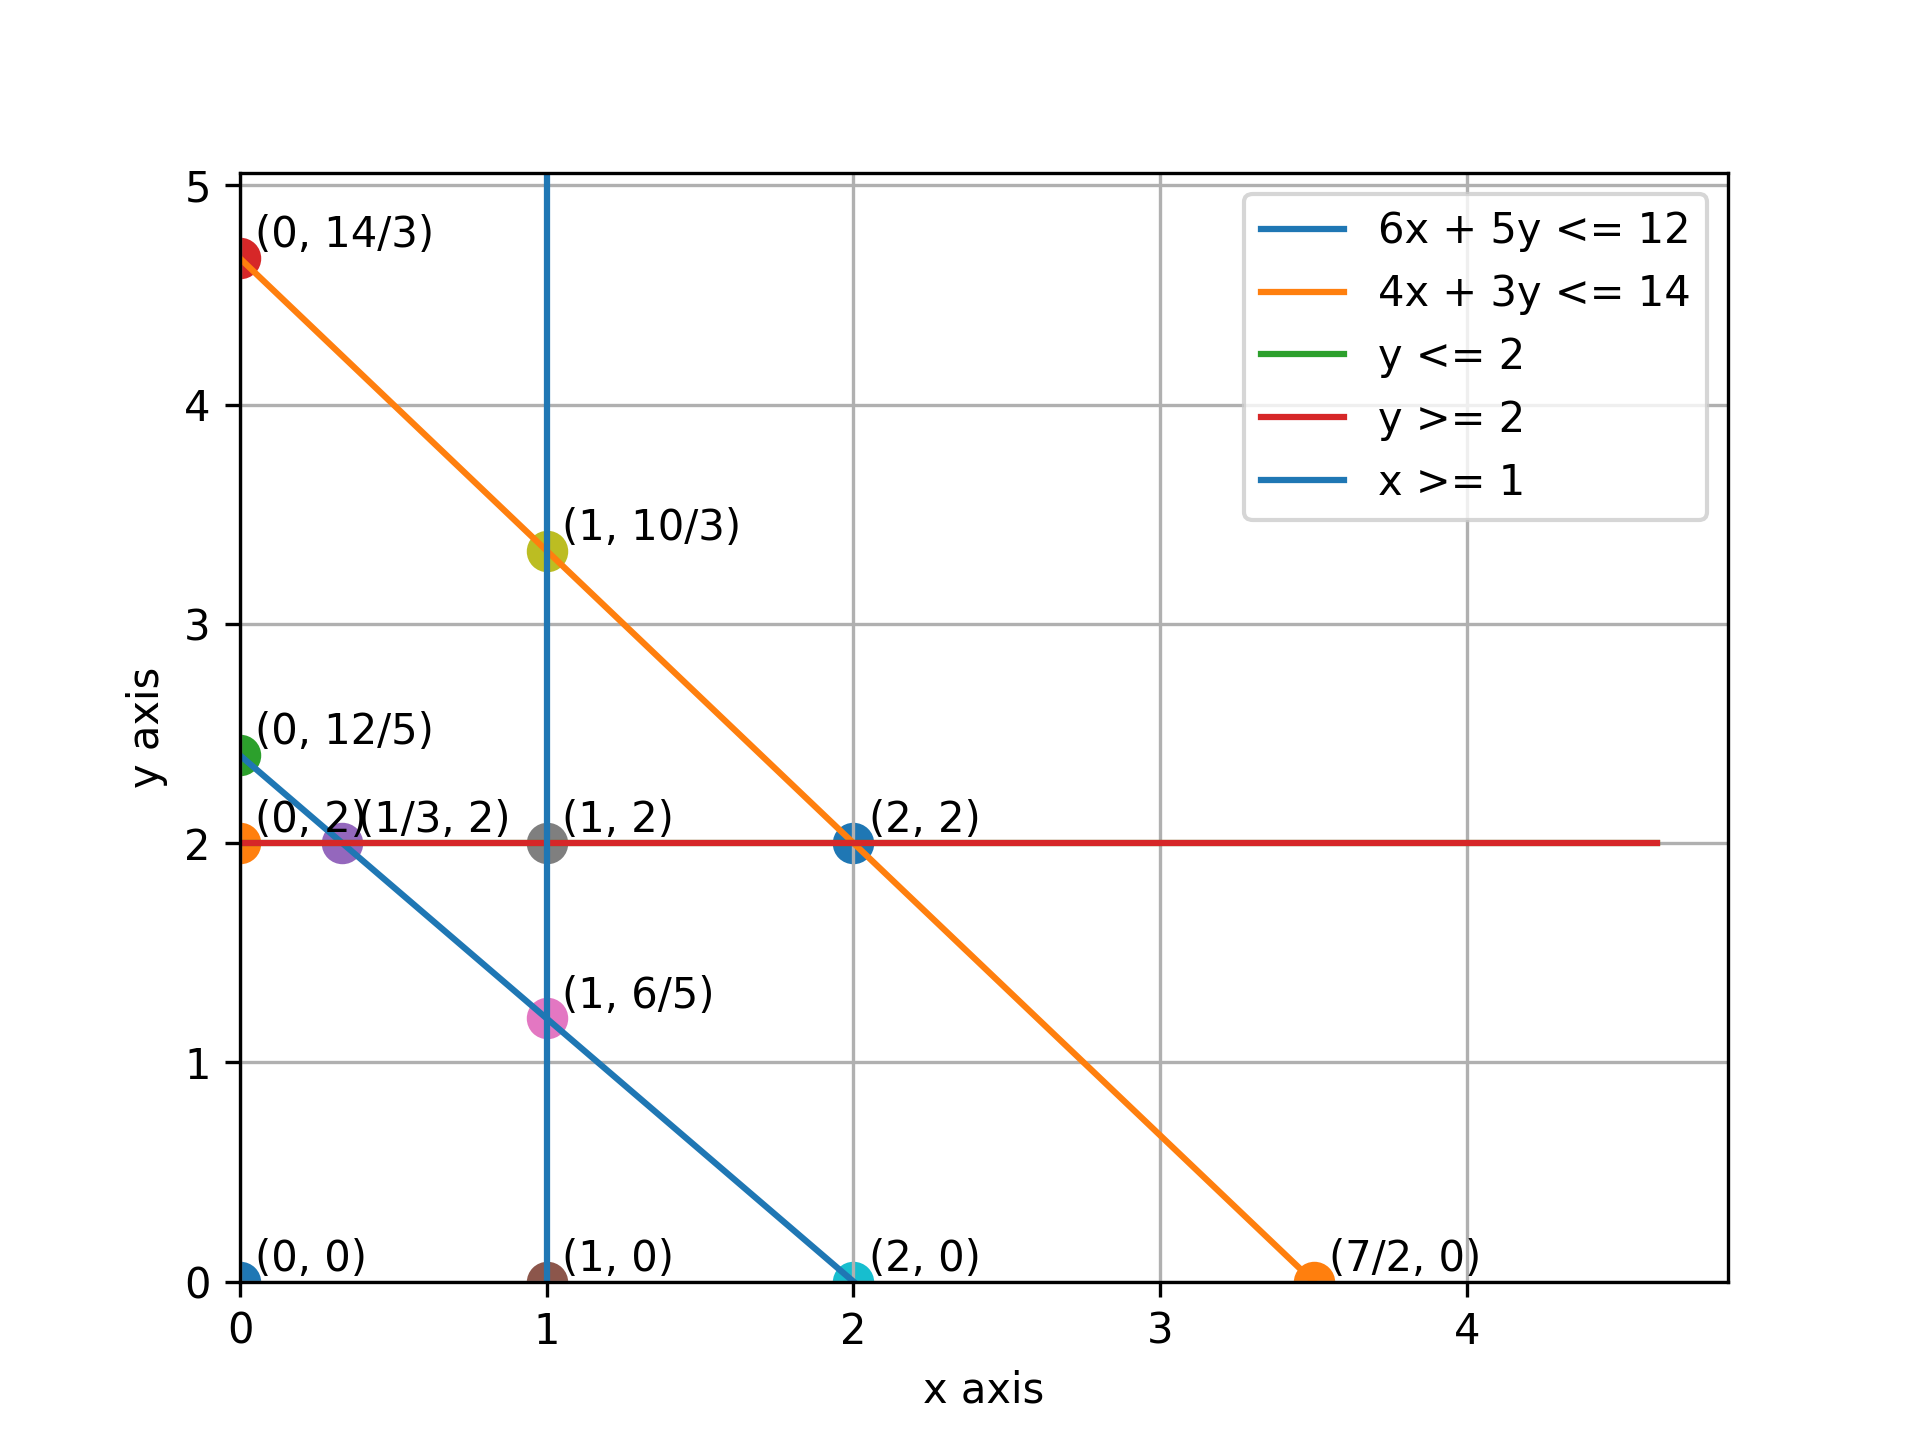
\includegraphics[width=0.6\textwidth]{outputs/ipp3/graph7.png}
\end{center}
Infeasible Solution\\
\begin{align*}
\text{Maximize} \quad & 2x + 3y\\
\text{subject to} \quad
& 6x + 5y\le12\\
& 4x + 3y\le14\\
& y\le2\\
& x\ge1\\
& y\le1\\
& x\le1\\
& x\ge0,\; y\ge0\end{align*}
\begin{align*}
6x + 5y=12\end{align*}
\begin{align*}
4x + 3y=14\end{align*}
Gauss Elimination:\\
Echelon Form:\\
\begin{align*}
\left(
\begin{array}{cc|c}
6 & 5 & 12\\
4 & 3 & 14\\
\end{array}
\right)_{2\times 3}
\end{align*}
\begin{align*}
\left(
\begin{array}{cc|c}
6 & 5 & 12\\
0 & -\frac{1}{3} & 6\\
\end{array}
\right)_{2\times 3}
\end{align*}
\begin{align*}
\left(
\begin{array}{cc|c}
6 & 5 & 12\\
0 & -\frac{1}{3} & 6\\
\end{array}
\right)_{2\times 3}
\end{align*}
\begin{align*}
x=17\end{align*}
\begin{align*}
y=-18\end{align*}
\begin{align*}
6x + 5y=12\end{align*}
\begin{align*}
y=2\end{align*}
Gauss Elimination:\\
Echelon Form:\\
\begin{align*}
\left(
\begin{array}{cc|c}
6 & 5 & 12\\
0 & 1 & 2\\
\end{array}
\right)_{2\times 3}
\end{align*}
\begin{align*}
\left(
\begin{array}{cc|c}
6 & 5 & 12\\
0 & 1 & 2\\
\end{array}
\right)_{2\times 3}
\end{align*}
\begin{align*}
\left(
\begin{array}{cc|c}
6 & 5 & 12\\
0 & 1 & 2\\
\end{array}
\right)_{2\times 3}
\end{align*}
\begin{align*}
x=\frac{1}{3}\end{align*}
\begin{align*}
y=2\end{align*}
\begin{align*}
6x + 5y=12\end{align*}
\begin{align*}
x=1\end{align*}
Gauss Elimination:\\
Echelon Form:\\
\begin{align*}
\left(
\begin{array}{cc|c}
6 & 5 & 12\\
1 & 0 & 1\\
\end{array}
\right)_{2\times 3}
\end{align*}
\begin{align*}
\left(
\begin{array}{cc|c}
6 & 5 & 12\\
0 & -\frac{5}{6} & -1\\
\end{array}
\right)_{2\times 3}
\end{align*}
\begin{align*}
\left(
\begin{array}{cc|c}
6 & 5 & 12\\
0 & -\frac{5}{6} & -1\\
\end{array}
\right)_{2\times 3}
\end{align*}
\begin{align*}
x=1\end{align*}
\begin{align*}
y=\frac{6}{5}\end{align*}
\begin{align*}
6x + 5y=12\end{align*}
\begin{align*}
y=1\end{align*}
Gauss Elimination:\\
Echelon Form:\\
\begin{align*}
\left(
\begin{array}{cc|c}
6 & 5 & 12\\
0 & 1 & 1\\
\end{array}
\right)_{2\times 3}
\end{align*}
\begin{align*}
\left(
\begin{array}{cc|c}
6 & 5 & 12\\
0 & 1 & 1\\
\end{array}
\right)_{2\times 3}
\end{align*}
\begin{align*}
\left(
\begin{array}{cc|c}
6 & 5 & 12\\
0 & 1 & 1\\
\end{array}
\right)_{2\times 3}
\end{align*}
\begin{align*}
x=\frac{7}{6}\end{align*}
\begin{align*}
y=1\end{align*}
\begin{align*}
6x + 5y=12\end{align*}
\begin{align*}
x=1\end{align*}
Gauss Elimination:\\
Echelon Form:\\
\begin{align*}
\left(
\begin{array}{cc|c}
6 & 5 & 12\\
1 & 0 & 1\\
\end{array}
\right)_{2\times 3}
\end{align*}
\begin{align*}
\left(
\begin{array}{cc|c}
6 & 5 & 12\\
0 & -\frac{5}{6} & -1\\
\end{array}
\right)_{2\times 3}
\end{align*}
\begin{align*}
\left(
\begin{array}{cc|c}
6 & 5 & 12\\
0 & -\frac{5}{6} & -1\\
\end{array}
\right)_{2\times 3}
\end{align*}
\begin{align*}
x=1\end{align*}
\begin{align*}
y=\frac{6}{5}\end{align*}
\begin{align*}
4x + 3y=14\end{align*}
\begin{align*}
y=2\end{align*}
Gauss Elimination:\\
Echelon Form:\\
\begin{align*}
\left(
\begin{array}{cc|c}
4 & 3 & 14\\
0 & 1 & 2\\
\end{array}
\right)_{2\times 3}
\end{align*}
\begin{align*}
\left(
\begin{array}{cc|c}
4 & 3 & 14\\
0 & 1 & 2\\
\end{array}
\right)_{2\times 3}
\end{align*}
\begin{align*}
\left(
\begin{array}{cc|c}
4 & 3 & 14\\
0 & 1 & 2\\
\end{array}
\right)_{2\times 3}
\end{align*}
\begin{align*}
x=2\end{align*}
\begin{align*}
y=2\end{align*}
\begin{align*}
4x + 3y=14\end{align*}
\begin{align*}
x=1\end{align*}
Gauss Elimination:\\
Echelon Form:\\
\begin{align*}
\left(
\begin{array}{cc|c}
4 & 3 & 14\\
1 & 0 & 1\\
\end{array}
\right)_{2\times 3}
\end{align*}
\begin{align*}
\left(
\begin{array}{cc|c}
4 & 3 & 14\\
0 & -\frac{3}{4} & -\frac{5}{2}\\
\end{array}
\right)_{2\times 3}
\end{align*}
\begin{align*}
\left(
\begin{array}{cc|c}
4 & 3 & 14\\
0 & -\frac{3}{4} & -\frac{5}{2}\\
\end{array}
\right)_{2\times 3}
\end{align*}
\begin{align*}
x=1\end{align*}
\begin{align*}
y=\frac{10}{3}\end{align*}
\begin{align*}
4x + 3y=14\end{align*}
\begin{align*}
y=1\end{align*}
Gauss Elimination:\\
Echelon Form:\\
\begin{align*}
\left(
\begin{array}{cc|c}
4 & 3 & 14\\
0 & 1 & 1\\
\end{array}
\right)_{2\times 3}
\end{align*}
\begin{align*}
\left(
\begin{array}{cc|c}
4 & 3 & 14\\
0 & 1 & 1\\
\end{array}
\right)_{2\times 3}
\end{align*}
\begin{align*}
\left(
\begin{array}{cc|c}
4 & 3 & 14\\
0 & 1 & 1\\
\end{array}
\right)_{2\times 3}
\end{align*}
\begin{align*}
x=\frac{11}{4}\end{align*}
\begin{align*}
y=1\end{align*}
\begin{align*}
4x + 3y=14\end{align*}
\begin{align*}
x=1\end{align*}
Gauss Elimination:\\
Echelon Form:\\
\begin{align*}
\left(
\begin{array}{cc|c}
4 & 3 & 14\\
1 & 0 & 1\\
\end{array}
\right)_{2\times 3}
\end{align*}
\begin{align*}
\left(
\begin{array}{cc|c}
4 & 3 & 14\\
0 & -\frac{3}{4} & -\frac{5}{2}\\
\end{array}
\right)_{2\times 3}
\end{align*}
\begin{align*}
\left(
\begin{array}{cc|c}
4 & 3 & 14\\
0 & -\frac{3}{4} & -\frac{5}{2}\\
\end{array}
\right)_{2\times 3}
\end{align*}
\begin{align*}
x=1\end{align*}
\begin{align*}
y=\frac{10}{3}\end{align*}
\begin{align*}
y=2\end{align*}
\begin{align*}
x=1\end{align*}
Gauss Elimination:\\
Echelon Form:\\
\begin{align*}
\left(
\begin{array}{cc|c}
0 & 1 & 2\\
1 & 0 & 1\\
\end{array}
\right)_{2\times 3}
\end{align*}
\begin{align*}
\left(
\begin{array}{cc|c}
1 & 0 & 1\\
0 & 1 & 2\\
\end{array}
\right)_{2\times 3}
\end{align*}
\begin{align*}
\left(
\begin{array}{cc|c}
1 & 0 & 1\\
0 & 1 & 2\\
\end{array}
\right)_{2\times 3}
\end{align*}
\begin{align*}
x=1\end{align*}
\begin{align*}
y=2\end{align*}
\begin{align*}
y=2\end{align*}
\begin{align*}
y=1\end{align*}
Gauss Elimination:\\
Echelon Form:\\
\begin{align*}
\left(
\begin{array}{c|c}
1 & 2\\
1 & 1\\
\end{array}
\right)_{2\times 2}
\end{align*}
\begin{align*}
\left(
\begin{array}{c|c}
1 & 2\\
0 & -1\\
\end{array}
\right)_{2\times 2}
\end{align*}
\begin{align*}
\left(
\begin{array}{c|c}
1 & 2\\
0 & -1\\
\end{array}
\right)_{2\times 2}
\end{align*}
No solution\\
\begin{align*}
y=2\end{align*}
\begin{align*}
x=1\end{align*}
Gauss Elimination:\\
Echelon Form:\\
\begin{align*}
\left(
\begin{array}{cc|c}
0 & 1 & 2\\
1 & 0 & 1\\
\end{array}
\right)_{2\times 3}
\end{align*}
\begin{align*}
\left(
\begin{array}{cc|c}
1 & 0 & 1\\
0 & 1 & 2\\
\end{array}
\right)_{2\times 3}
\end{align*}
\begin{align*}
\left(
\begin{array}{cc|c}
1 & 0 & 1\\
0 & 1 & 2\\
\end{array}
\right)_{2\times 3}
\end{align*}
\begin{align*}
x=1\end{align*}
\begin{align*}
y=2\end{align*}
\begin{align*}
x=1\end{align*}
\begin{align*}
y=1\end{align*}
Gauss Elimination:\\
Echelon Form:\\
\begin{align*}
\left(
\begin{array}{cc|c}
1 & 0 & 1\\
0 & 1 & 1\\
\end{array}
\right)_{2\times 3}
\end{align*}
\begin{align*}
\left(
\begin{array}{cc|c}
1 & 0 & 1\\
0 & 1 & 1\\
\end{array}
\right)_{2\times 3}
\end{align*}
\begin{align*}
\left(
\begin{array}{cc|c}
1 & 0 & 1\\
0 & 1 & 1\\
\end{array}
\right)_{2\times 3}
\end{align*}
\begin{align*}
x=1\end{align*}
\begin{align*}
y=1\end{align*}
\begin{align*}
x=1\end{align*}
\begin{align*}
x=1\end{align*}
Gauss Elimination:\\
Echelon Form:\\
\begin{align*}
\left(
\begin{array}{c|c}
1 & 1\\
1 & 1\\
\end{array}
\right)_{2\times 2}
\end{align*}
\begin{align*}
\left(
\begin{array}{c|c}
1 & 1\\
0 & 0\\
\end{array}
\right)_{2\times 2}
\end{align*}
Infinitely many solutions\\
\begin{align*}
y=1\end{align*}
\begin{align*}
x=1\end{align*}
Gauss Elimination:\\
Echelon Form:\\
\begin{align*}
\left(
\begin{array}{cc|c}
0 & 1 & 1\\
1 & 0 & 1\\
\end{array}
\right)_{2\times 3}
\end{align*}
\begin{align*}
\left(
\begin{array}{cc|c}
1 & 0 & 1\\
0 & 1 & 1\\
\end{array}
\right)_{2\times 3}
\end{align*}
\begin{align*}
\left(
\begin{array}{cc|c}
1 & 0 & 1\\
0 & 1 & 1\\
\end{array}
\right)_{2\times 3}
\end{align*}
\begin{align*}
x=1\end{align*}
\begin{align*}
y=1\end{align*}
\begin{center}
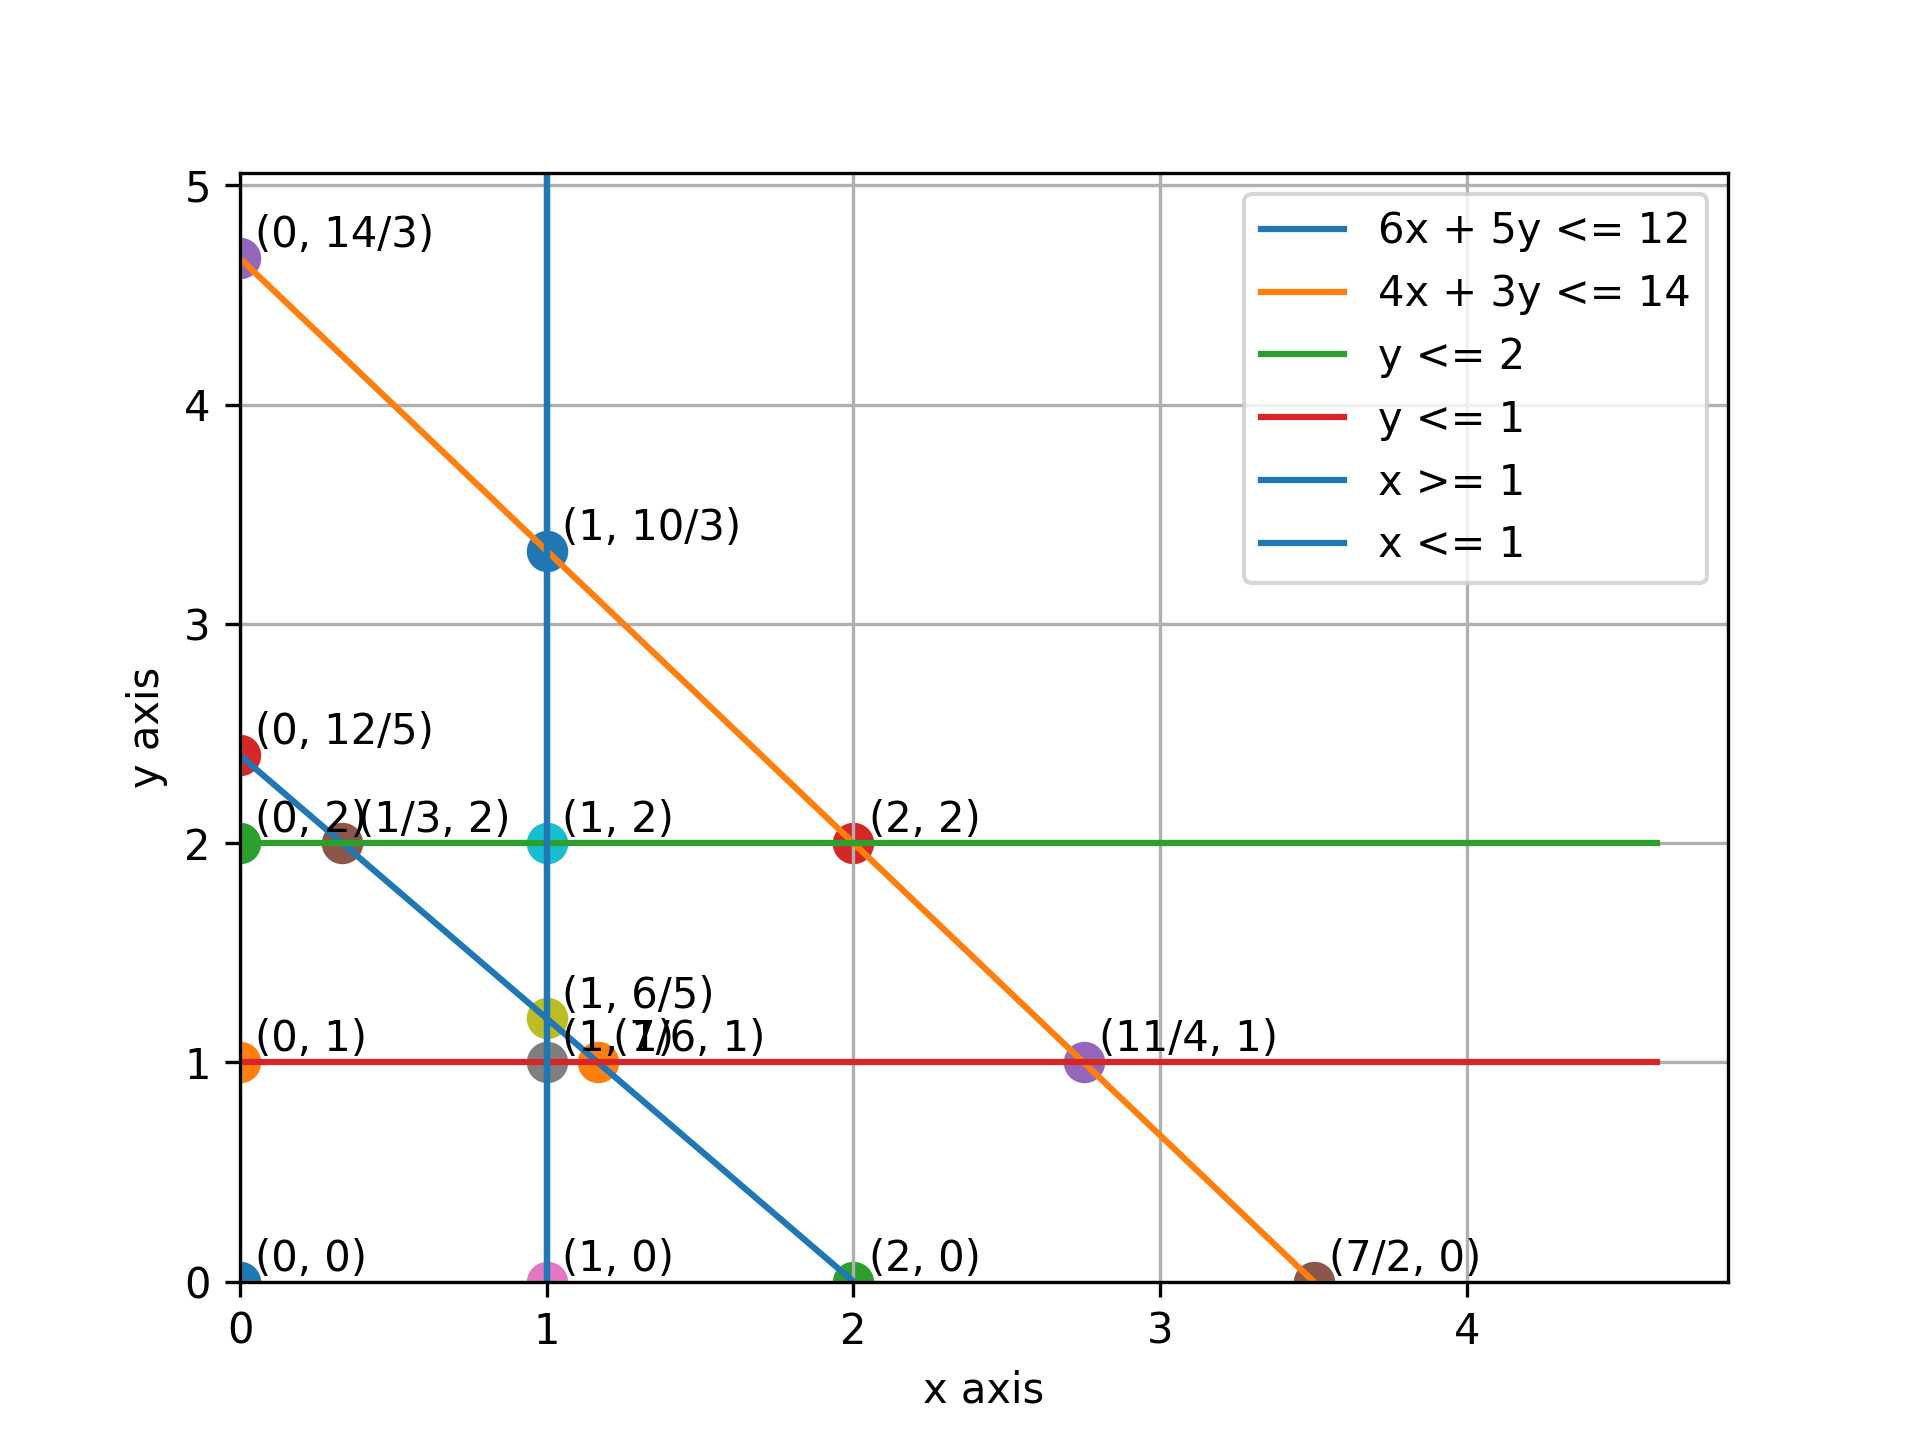
\includegraphics[width=0.6\textwidth]{outputs/ipp3/graph8.png}
\end{center}
\begin{align*}
Z=5\end{align*}
\begin{align*}
x=1\end{align*}
\begin{align*}
y=1\end{align*}
\begin{align*}
\text{Maximize} \quad & 2x + 3y\\
\text{subject to} \quad
& 6x + 5y\le12\\
& 4x + 3y\le14\\
& y\le2\\
& x\ge1\\
& y\le1\\
& x\ge2\\
& x\ge0,\; y\ge0\end{align*}
\begin{align*}
6x + 5y=12\end{align*}
\begin{align*}
4x + 3y=14\end{align*}
Gauss Elimination:\\
Echelon Form:\\
\begin{align*}
\left(
\begin{array}{cc|c}
6 & 5 & 12\\
4 & 3 & 14\\
\end{array}
\right)_{2\times 3}
\end{align*}
\begin{align*}
\left(
\begin{array}{cc|c}
6 & 5 & 12\\
0 & -\frac{1}{3} & 6\\
\end{array}
\right)_{2\times 3}
\end{align*}
\begin{align*}
\left(
\begin{array}{cc|c}
6 & 5 & 12\\
0 & -\frac{1}{3} & 6\\
\end{array}
\right)_{2\times 3}
\end{align*}
\begin{align*}
x=17\end{align*}
\begin{align*}
y=-18\end{align*}
\begin{align*}
6x + 5y=12\end{align*}
\begin{align*}
y=2\end{align*}
Gauss Elimination:\\
Echelon Form:\\
\begin{align*}
\left(
\begin{array}{cc|c}
6 & 5 & 12\\
0 & 1 & 2\\
\end{array}
\right)_{2\times 3}
\end{align*}
\begin{align*}
\left(
\begin{array}{cc|c}
6 & 5 & 12\\
0 & 1 & 2\\
\end{array}
\right)_{2\times 3}
\end{align*}
\begin{align*}
\left(
\begin{array}{cc|c}
6 & 5 & 12\\
0 & 1 & 2\\
\end{array}
\right)_{2\times 3}
\end{align*}
\begin{align*}
x=\frac{1}{3}\end{align*}
\begin{align*}
y=2\end{align*}
\begin{align*}
6x + 5y=12\end{align*}
\begin{align*}
x=1\end{align*}
Gauss Elimination:\\
Echelon Form:\\
\begin{align*}
\left(
\begin{array}{cc|c}
6 & 5 & 12\\
1 & 0 & 1\\
\end{array}
\right)_{2\times 3}
\end{align*}
\begin{align*}
\left(
\begin{array}{cc|c}
6 & 5 & 12\\
0 & -\frac{5}{6} & -1\\
\end{array}
\right)_{2\times 3}
\end{align*}
\begin{align*}
\left(
\begin{array}{cc|c}
6 & 5 & 12\\
0 & -\frac{5}{6} & -1\\
\end{array}
\right)_{2\times 3}
\end{align*}
\begin{align*}
x=1\end{align*}
\begin{align*}
y=\frac{6}{5}\end{align*}
\begin{align*}
6x + 5y=12\end{align*}
\begin{align*}
y=1\end{align*}
Gauss Elimination:\\
Echelon Form:\\
\begin{align*}
\left(
\begin{array}{cc|c}
6 & 5 & 12\\
0 & 1 & 1\\
\end{array}
\right)_{2\times 3}
\end{align*}
\begin{align*}
\left(
\begin{array}{cc|c}
6 & 5 & 12\\
0 & 1 & 1\\
\end{array}
\right)_{2\times 3}
\end{align*}
\begin{align*}
\left(
\begin{array}{cc|c}
6 & 5 & 12\\
0 & 1 & 1\\
\end{array}
\right)_{2\times 3}
\end{align*}
\begin{align*}
x=\frac{7}{6}\end{align*}
\begin{align*}
y=1\end{align*}
\begin{align*}
6x + 5y=12\end{align*}
\begin{align*}
x=2\end{align*}
Gauss Elimination:\\
Echelon Form:\\
\begin{align*}
\left(
\begin{array}{cc|c}
6 & 5 & 12\\
1 & 0 & 2\\
\end{array}
\right)_{2\times 3}
\end{align*}
\begin{align*}
\left(
\begin{array}{cc|c}
6 & 5 & 12\\
0 & -\frac{5}{6} & 0\\
\end{array}
\right)_{2\times 3}
\end{align*}
\begin{align*}
\left(
\begin{array}{cc|c}
6 & 5 & 12\\
0 & -\frac{5}{6} & 0\\
\end{array}
\right)_{2\times 3}
\end{align*}
\begin{align*}
x=2\end{align*}
\begin{align*}
y=0\end{align*}
\begin{align*}
4x + 3y=14\end{align*}
\begin{align*}
y=2\end{align*}
Gauss Elimination:\\
Echelon Form:\\
\begin{align*}
\left(
\begin{array}{cc|c}
4 & 3 & 14\\
0 & 1 & 2\\
\end{array}
\right)_{2\times 3}
\end{align*}
\begin{align*}
\left(
\begin{array}{cc|c}
4 & 3 & 14\\
0 & 1 & 2\\
\end{array}
\right)_{2\times 3}
\end{align*}
\begin{align*}
\left(
\begin{array}{cc|c}
4 & 3 & 14\\
0 & 1 & 2\\
\end{array}
\right)_{2\times 3}
\end{align*}
\begin{align*}
x=2\end{align*}
\begin{align*}
y=2\end{align*}
\begin{align*}
4x + 3y=14\end{align*}
\begin{align*}
x=1\end{align*}
Gauss Elimination:\\
Echelon Form:\\
\begin{align*}
\left(
\begin{array}{cc|c}
4 & 3 & 14\\
1 & 0 & 1\\
\end{array}
\right)_{2\times 3}
\end{align*}
\begin{align*}
\left(
\begin{array}{cc|c}
4 & 3 & 14\\
0 & -\frac{3}{4} & -\frac{5}{2}\\
\end{array}
\right)_{2\times 3}
\end{align*}
\begin{align*}
\left(
\begin{array}{cc|c}
4 & 3 & 14\\
0 & -\frac{3}{4} & -\frac{5}{2}\\
\end{array}
\right)_{2\times 3}
\end{align*}
\begin{align*}
x=1\end{align*}
\begin{align*}
y=\frac{10}{3}\end{align*}
\begin{align*}
4x + 3y=14\end{align*}
\begin{align*}
y=1\end{align*}
Gauss Elimination:\\
Echelon Form:\\
\begin{align*}
\left(
\begin{array}{cc|c}
4 & 3 & 14\\
0 & 1 & 1\\
\end{array}
\right)_{2\times 3}
\end{align*}
\begin{align*}
\left(
\begin{array}{cc|c}
4 & 3 & 14\\
0 & 1 & 1\\
\end{array}
\right)_{2\times 3}
\end{align*}
\begin{align*}
\left(
\begin{array}{cc|c}
4 & 3 & 14\\
0 & 1 & 1\\
\end{array}
\right)_{2\times 3}
\end{align*}
\begin{align*}
x=\frac{11}{4}\end{align*}
\begin{align*}
y=1\end{align*}
\begin{align*}
4x + 3y=14\end{align*}
\begin{align*}
x=2\end{align*}
Gauss Elimination:\\
Echelon Form:\\
\begin{align*}
\left(
\begin{array}{cc|c}
4 & 3 & 14\\
1 & 0 & 2\\
\end{array}
\right)_{2\times 3}
\end{align*}
\begin{align*}
\left(
\begin{array}{cc|c}
4 & 3 & 14\\
0 & -\frac{3}{4} & -\frac{3}{2}\\
\end{array}
\right)_{2\times 3}
\end{align*}
\begin{align*}
\left(
\begin{array}{cc|c}
4 & 3 & 14\\
0 & -\frac{3}{4} & -\frac{3}{2}\\
\end{array}
\right)_{2\times 3}
\end{align*}
\begin{align*}
x=2\end{align*}
\begin{align*}
y=2\end{align*}
\begin{align*}
y=2\end{align*}
\begin{align*}
x=1\end{align*}
Gauss Elimination:\\
Echelon Form:\\
\begin{align*}
\left(
\begin{array}{cc|c}
0 & 1 & 2\\
1 & 0 & 1\\
\end{array}
\right)_{2\times 3}
\end{align*}
\begin{align*}
\left(
\begin{array}{cc|c}
1 & 0 & 1\\
0 & 1 & 2\\
\end{array}
\right)_{2\times 3}
\end{align*}
\begin{align*}
\left(
\begin{array}{cc|c}
1 & 0 & 1\\
0 & 1 & 2\\
\end{array}
\right)_{2\times 3}
\end{align*}
\begin{align*}
x=1\end{align*}
\begin{align*}
y=2\end{align*}
\begin{align*}
y=2\end{align*}
\begin{align*}
y=1\end{align*}
Gauss Elimination:\\
Echelon Form:\\
\begin{align*}
\left(
\begin{array}{c|c}
1 & 2\\
1 & 1\\
\end{array}
\right)_{2\times 2}
\end{align*}
\begin{align*}
\left(
\begin{array}{c|c}
1 & 2\\
0 & -1\\
\end{array}
\right)_{2\times 2}
\end{align*}
\begin{align*}
\left(
\begin{array}{c|c}
1 & 2\\
0 & -1\\
\end{array}
\right)_{2\times 2}
\end{align*}
No solution\\
\begin{align*}
y=2\end{align*}
\begin{align*}
x=2\end{align*}
Gauss Elimination:\\
Echelon Form:\\
\begin{align*}
\left(
\begin{array}{cc|c}
0 & 1 & 2\\
1 & 0 & 2\\
\end{array}
\right)_{2\times 3}
\end{align*}
\begin{align*}
\left(
\begin{array}{cc|c}
1 & 0 & 2\\
0 & 1 & 2\\
\end{array}
\right)_{2\times 3}
\end{align*}
\begin{align*}
\left(
\begin{array}{cc|c}
1 & 0 & 2\\
0 & 1 & 2\\
\end{array}
\right)_{2\times 3}
\end{align*}
\begin{align*}
x=2\end{align*}
\begin{align*}
y=2\end{align*}
\begin{align*}
x=1\end{align*}
\begin{align*}
y=1\end{align*}
Gauss Elimination:\\
Echelon Form:\\
\begin{align*}
\left(
\begin{array}{cc|c}
1 & 0 & 1\\
0 & 1 & 1\\
\end{array}
\right)_{2\times 3}
\end{align*}
\begin{align*}
\left(
\begin{array}{cc|c}
1 & 0 & 1\\
0 & 1 & 1\\
\end{array}
\right)_{2\times 3}
\end{align*}
\begin{align*}
\left(
\begin{array}{cc|c}
1 & 0 & 1\\
0 & 1 & 1\\
\end{array}
\right)_{2\times 3}
\end{align*}
\begin{align*}
x=1\end{align*}
\begin{align*}
y=1\end{align*}
\begin{align*}
x=1\end{align*}
\begin{align*}
x=2\end{align*}
Gauss Elimination:\\
Echelon Form:\\
\begin{align*}
\left(
\begin{array}{c|c}
1 & 1\\
1 & 2\\
\end{array}
\right)_{2\times 2}
\end{align*}
\begin{align*}
\left(
\begin{array}{c|c}
1 & 1\\
0 & 1\\
\end{array}
\right)_{2\times 2}
\end{align*}
\begin{align*}
\left(
\begin{array}{c|c}
1 & 1\\
0 & 1\\
\end{array}
\right)_{2\times 2}
\end{align*}
No solution\\
\begin{align*}
y=1\end{align*}
\begin{align*}
x=2\end{align*}
Gauss Elimination:\\
Echelon Form:\\
\begin{align*}
\left(
\begin{array}{cc|c}
0 & 1 & 1\\
1 & 0 & 2\\
\end{array}
\right)_{2\times 3}
\end{align*}
\begin{align*}
\left(
\begin{array}{cc|c}
1 & 0 & 2\\
0 & 1 & 1\\
\end{array}
\right)_{2\times 3}
\end{align*}
\begin{align*}
\left(
\begin{array}{cc|c}
1 & 0 & 2\\
0 & 1 & 1\\
\end{array}
\right)_{2\times 3}
\end{align*}
\begin{align*}
x=2\end{align*}
\begin{align*}
y=1\end{align*}
\begin{center}
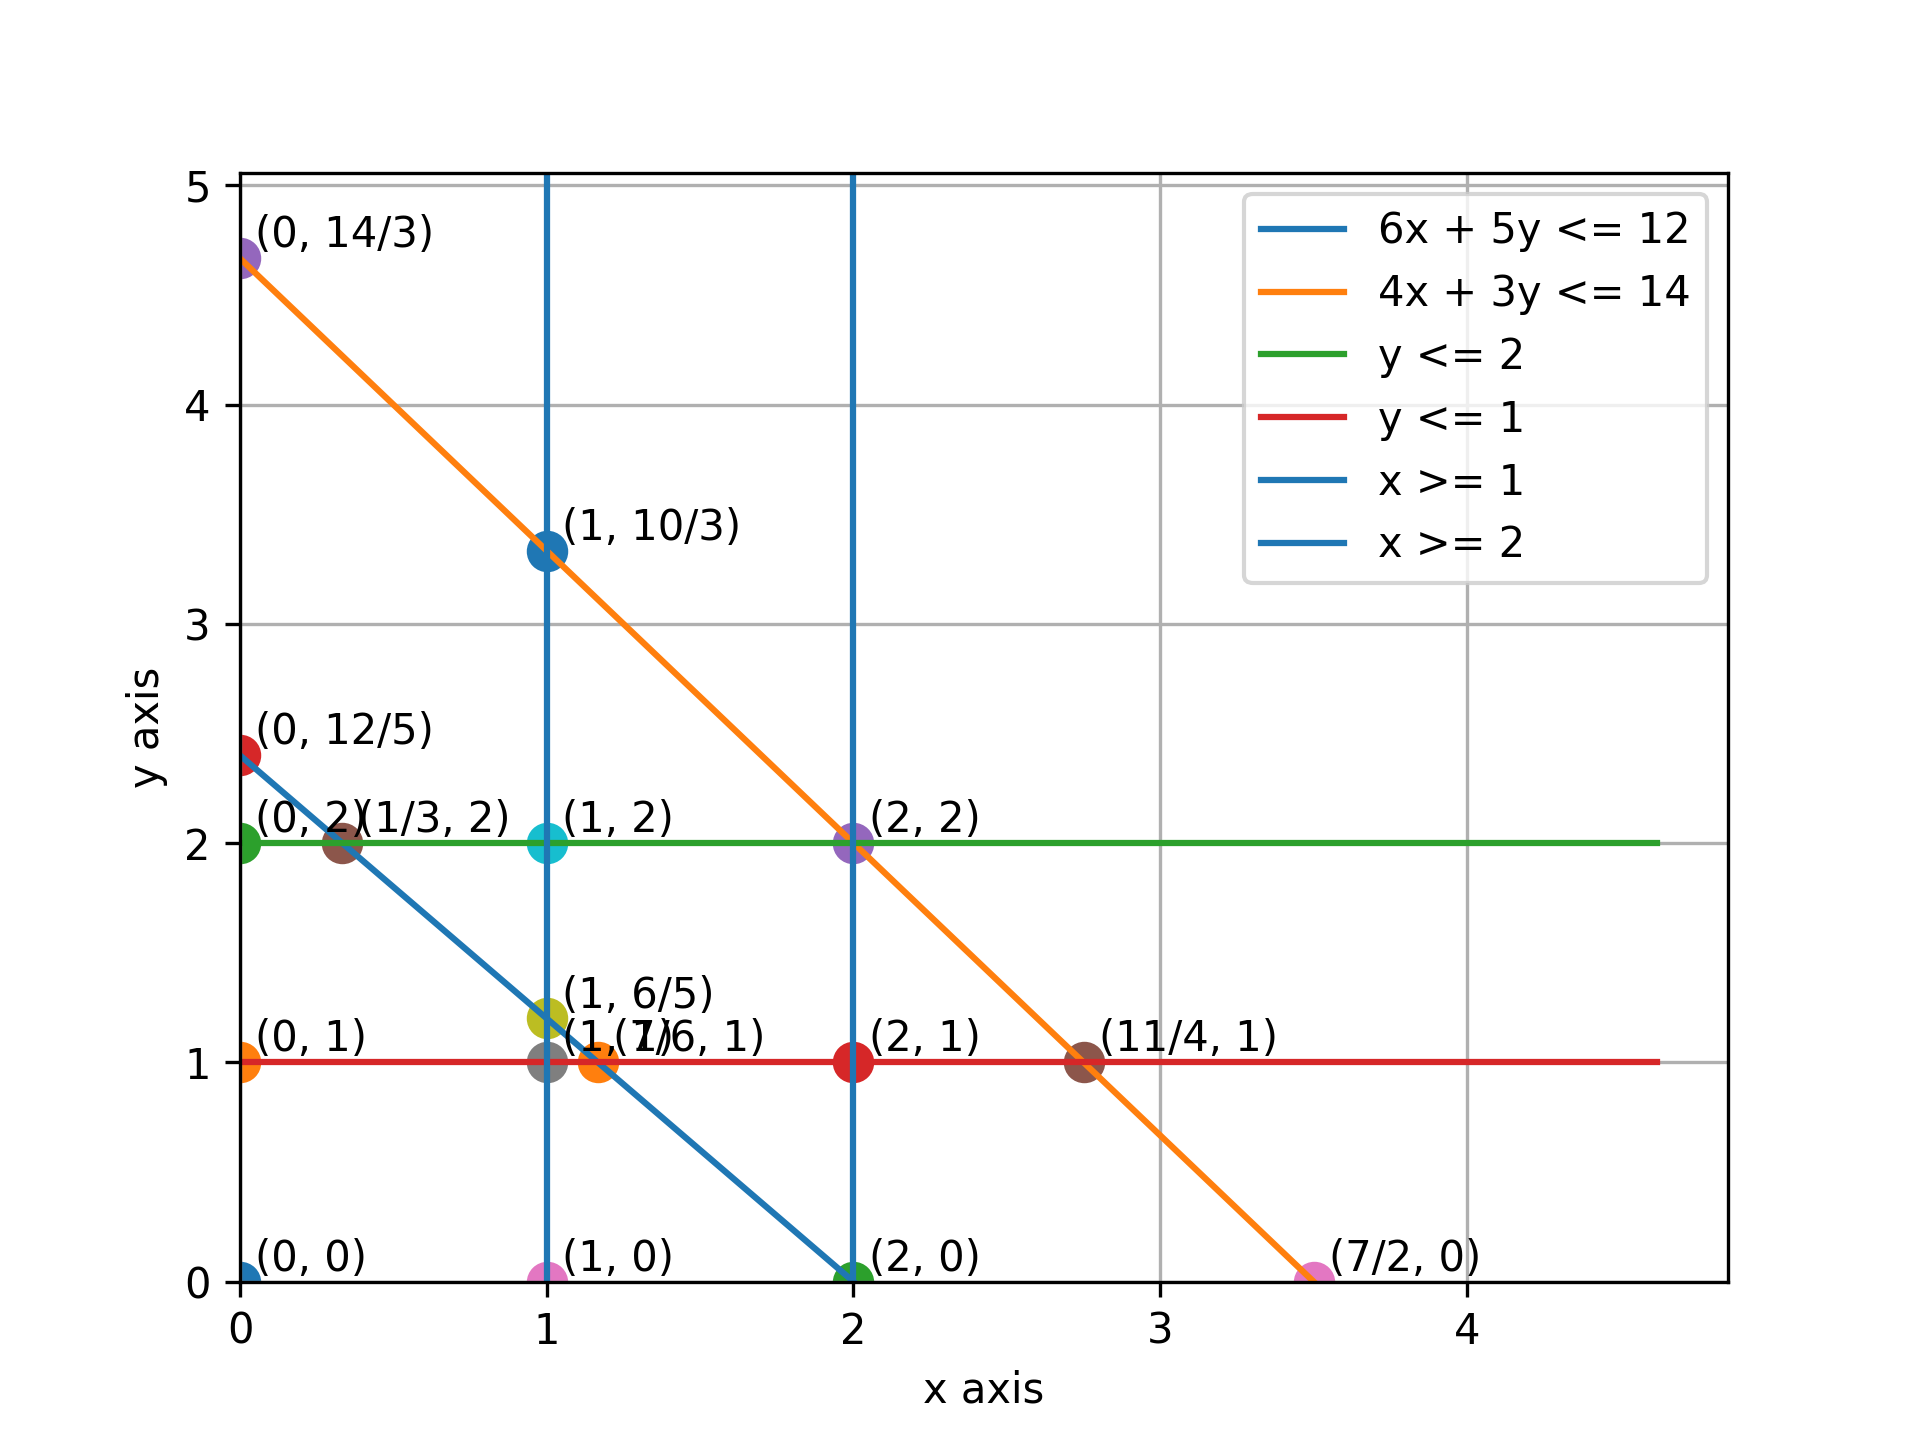
\includegraphics[width=0.6\textwidth]{outputs/ipp3/graph9.png}
\end{center}
\begin{align*}
Z=4\end{align*}
\begin{align*}
x=2\end{align*}
\begin{align*}
y=0\end{align*}
\begin{align*}
Z=6\end{align*}
\begin{align*}
x=0\end{align*}
\begin{align*}
y=2\end{align*}
\begin{align*}
\text{Maximize} \quad & 3x + 4y\\
\text{subject to} \quad
& 3x - y\le12\\
& 3x + 11y\le66\\
& x\ge0,\; y\ge0\end{align*}
\begin{align*}
3x - y=12\end{align*}
\begin{align*}
3x + 11y=66\end{align*}
Gauss Elimination:\\
Echelon Form:\\
\begin{align*}
\left(
\begin{array}{cc|c}
3 & -1 & 12\\
3 & 11 & 66\\
\end{array}
\right)_{2\times 3}
\end{align*}
\begin{align*}
\left(
\begin{array}{cc|c}
3 & -1 & 12\\
0 & 12 & 54\\
\end{array}
\right)_{2\times 3}
\end{align*}
\begin{align*}
\left(
\begin{array}{cc|c}
3 & -1 & 12\\
0 & 12 & 54\\
\end{array}
\right)_{2\times 3}
\end{align*}
\begin{align*}
x=\frac{11}{2}\end{align*}
\begin{align*}
y=\frac{9}{2}\end{align*}
\begin{center}
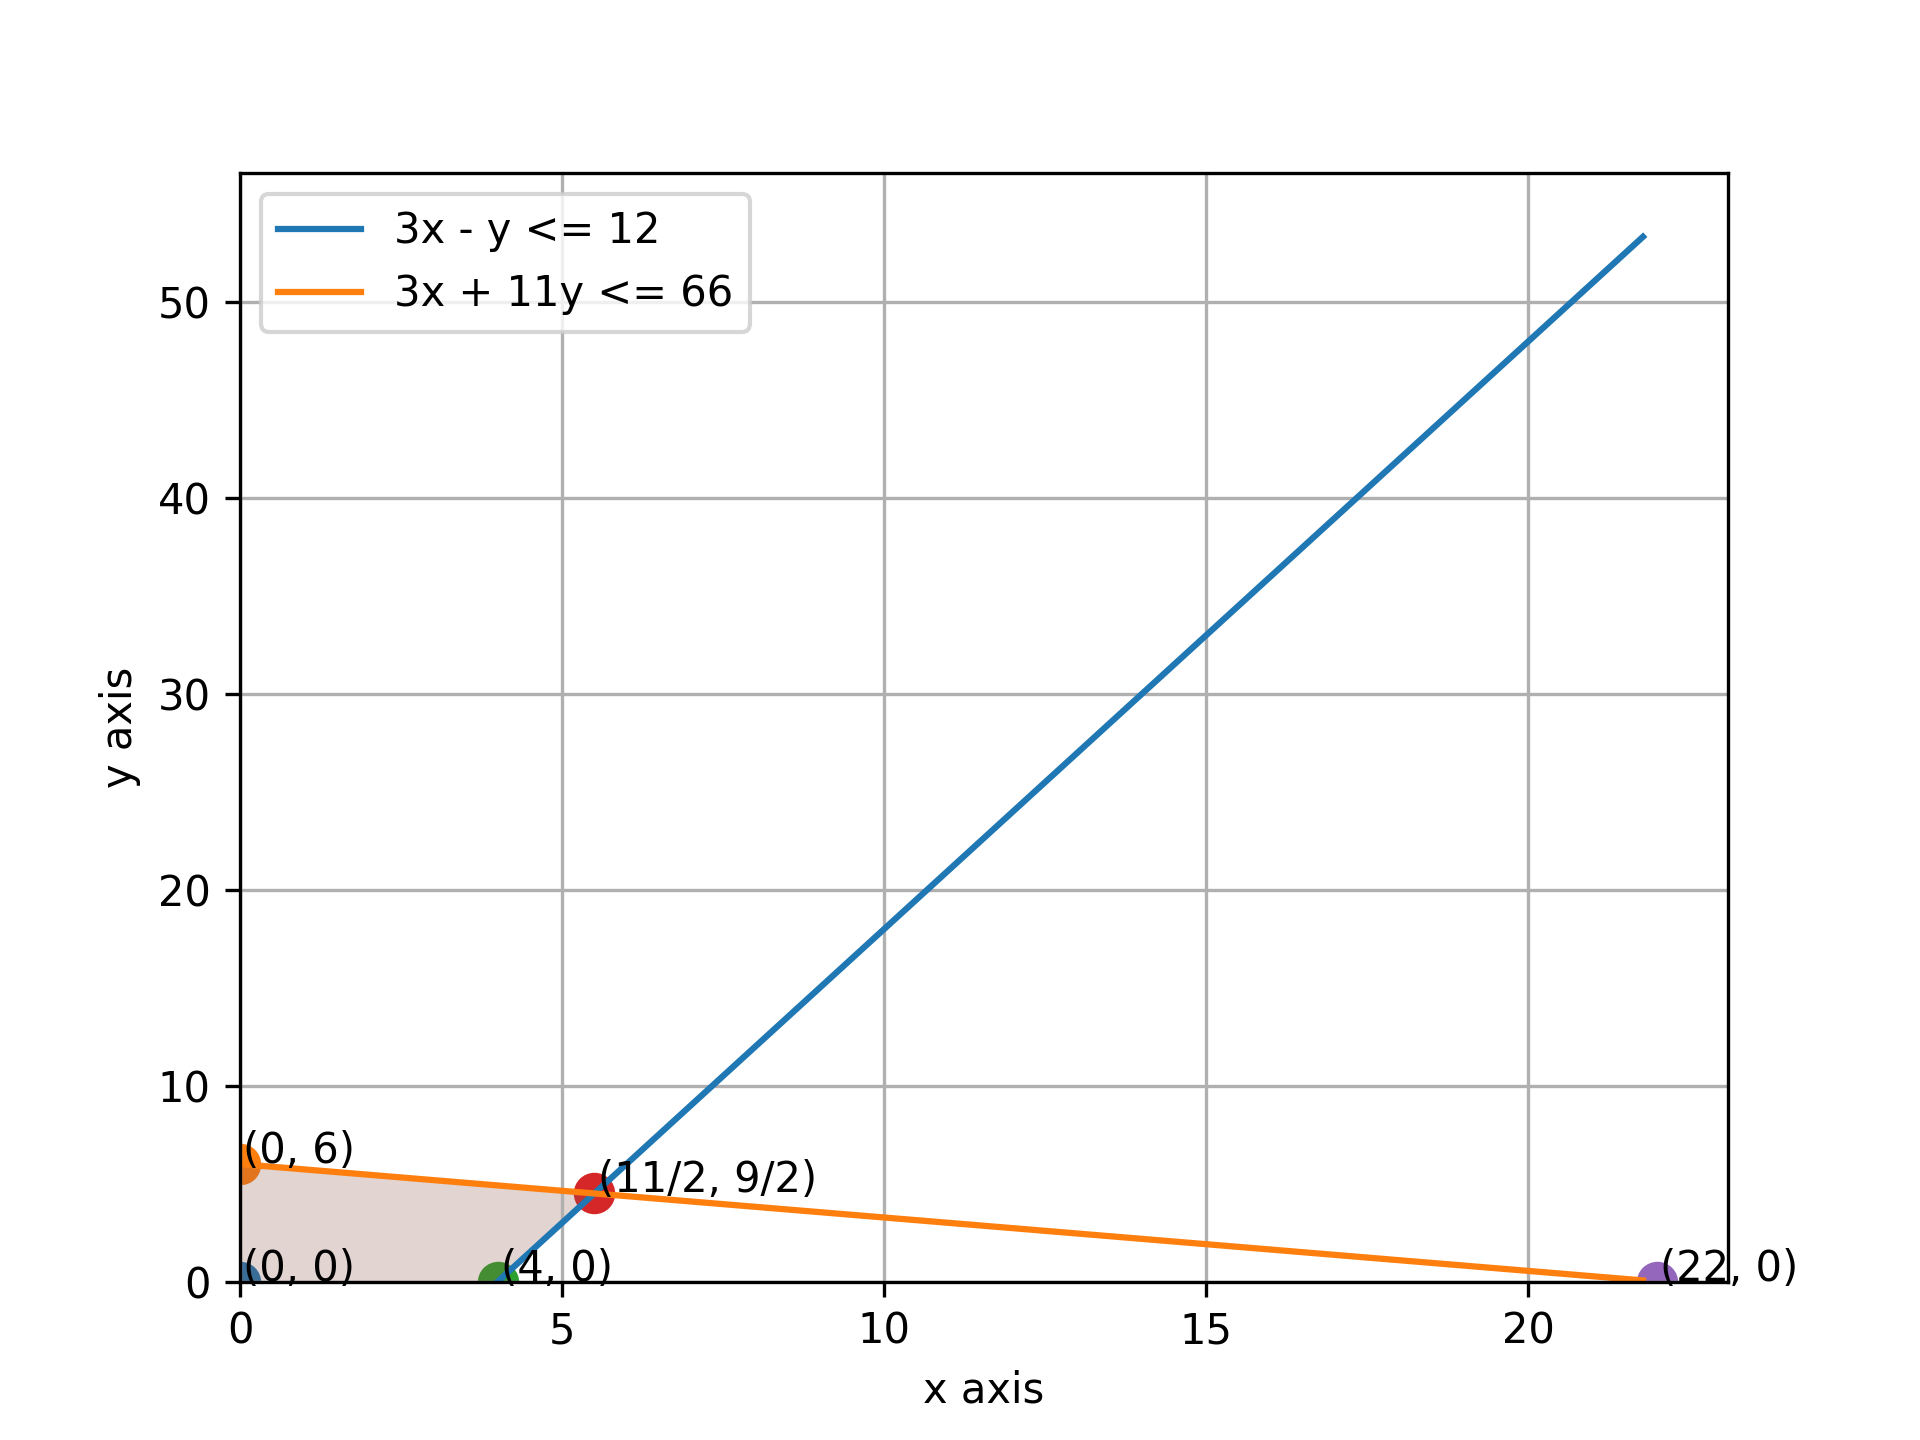
\includegraphics[width=0.6\textwidth]{outputs/ipp4/graph1.png}
\end{center}
\begin{align*}
Z=69\end{align*}
\begin{align*}
x=11\end{align*}
\begin{align*}
y=9\end{align*}
\begin{align*}
\text{Maximize} \quad & 3x + 4y\\
\text{subject to} \quad
& 3x - y\le12\\
& 3x + 11y\le66\\
& x\le5\\
& x\ge0,\; y\ge0\end{align*}
\begin{align*}
3x - y=12\end{align*}
\begin{align*}
3x + 11y=66\end{align*}
Gauss Elimination:\\
Echelon Form:\\
\begin{align*}
\left(
\begin{array}{cc|c}
3 & -1 & 12\\
3 & 11 & 66\\
\end{array}
\right)_{2\times 3}
\end{align*}
\begin{align*}
\left(
\begin{array}{cc|c}
3 & -1 & 12\\
0 & 12 & 54\\
\end{array}
\right)_{2\times 3}
\end{align*}
\begin{align*}
\left(
\begin{array}{cc|c}
3 & -1 & 12\\
0 & 12 & 54\\
\end{array}
\right)_{2\times 3}
\end{align*}
\begin{align*}
x=\frac{11}{2}\end{align*}
\begin{align*}
y=\frac{9}{2}\end{align*}
\begin{align*}
3x - y=12\end{align*}
\begin{align*}
x=5\end{align*}
Gauss Elimination:\\
Echelon Form:\\
\begin{align*}
\left(
\begin{array}{cc|c}
3 & -1 & 12\\
1 & 0 & 5\\
\end{array}
\right)_{2\times 3}
\end{align*}
\begin{align*}
\left(
\begin{array}{cc|c}
3 & -1 & 12\\
0 & \frac{1}{3} & 1\\
\end{array}
\right)_{2\times 3}
\end{align*}
\begin{align*}
\left(
\begin{array}{cc|c}
3 & -1 & 12\\
0 & \frac{1}{3} & 1\\
\end{array}
\right)_{2\times 3}
\end{align*}
\begin{align*}
x=5\end{align*}
\begin{align*}
y=3\end{align*}
\begin{align*}
3x + 11y=66\end{align*}
\begin{align*}
x=5\end{align*}
Gauss Elimination:\\
Echelon Form:\\
\begin{align*}
\left(
\begin{array}{cc|c}
3 & 11 & 66\\
1 & 0 & 5\\
\end{array}
\right)_{2\times 3}
\end{align*}
\begin{align*}
\left(
\begin{array}{cc|c}
3 & 11 & 66\\
0 & -\frac{11}{3} & -17\\
\end{array}
\right)_{2\times 3}
\end{align*}
\begin{align*}
\left(
\begin{array}{cc|c}
3 & 11 & 66\\
0 & -\frac{11}{3} & -17\\
\end{array}
\right)_{2\times 3}
\end{align*}
\begin{align*}
x=5\end{align*}
\begin{align*}
y=\frac{51}{11}\end{align*}
\begin{center}
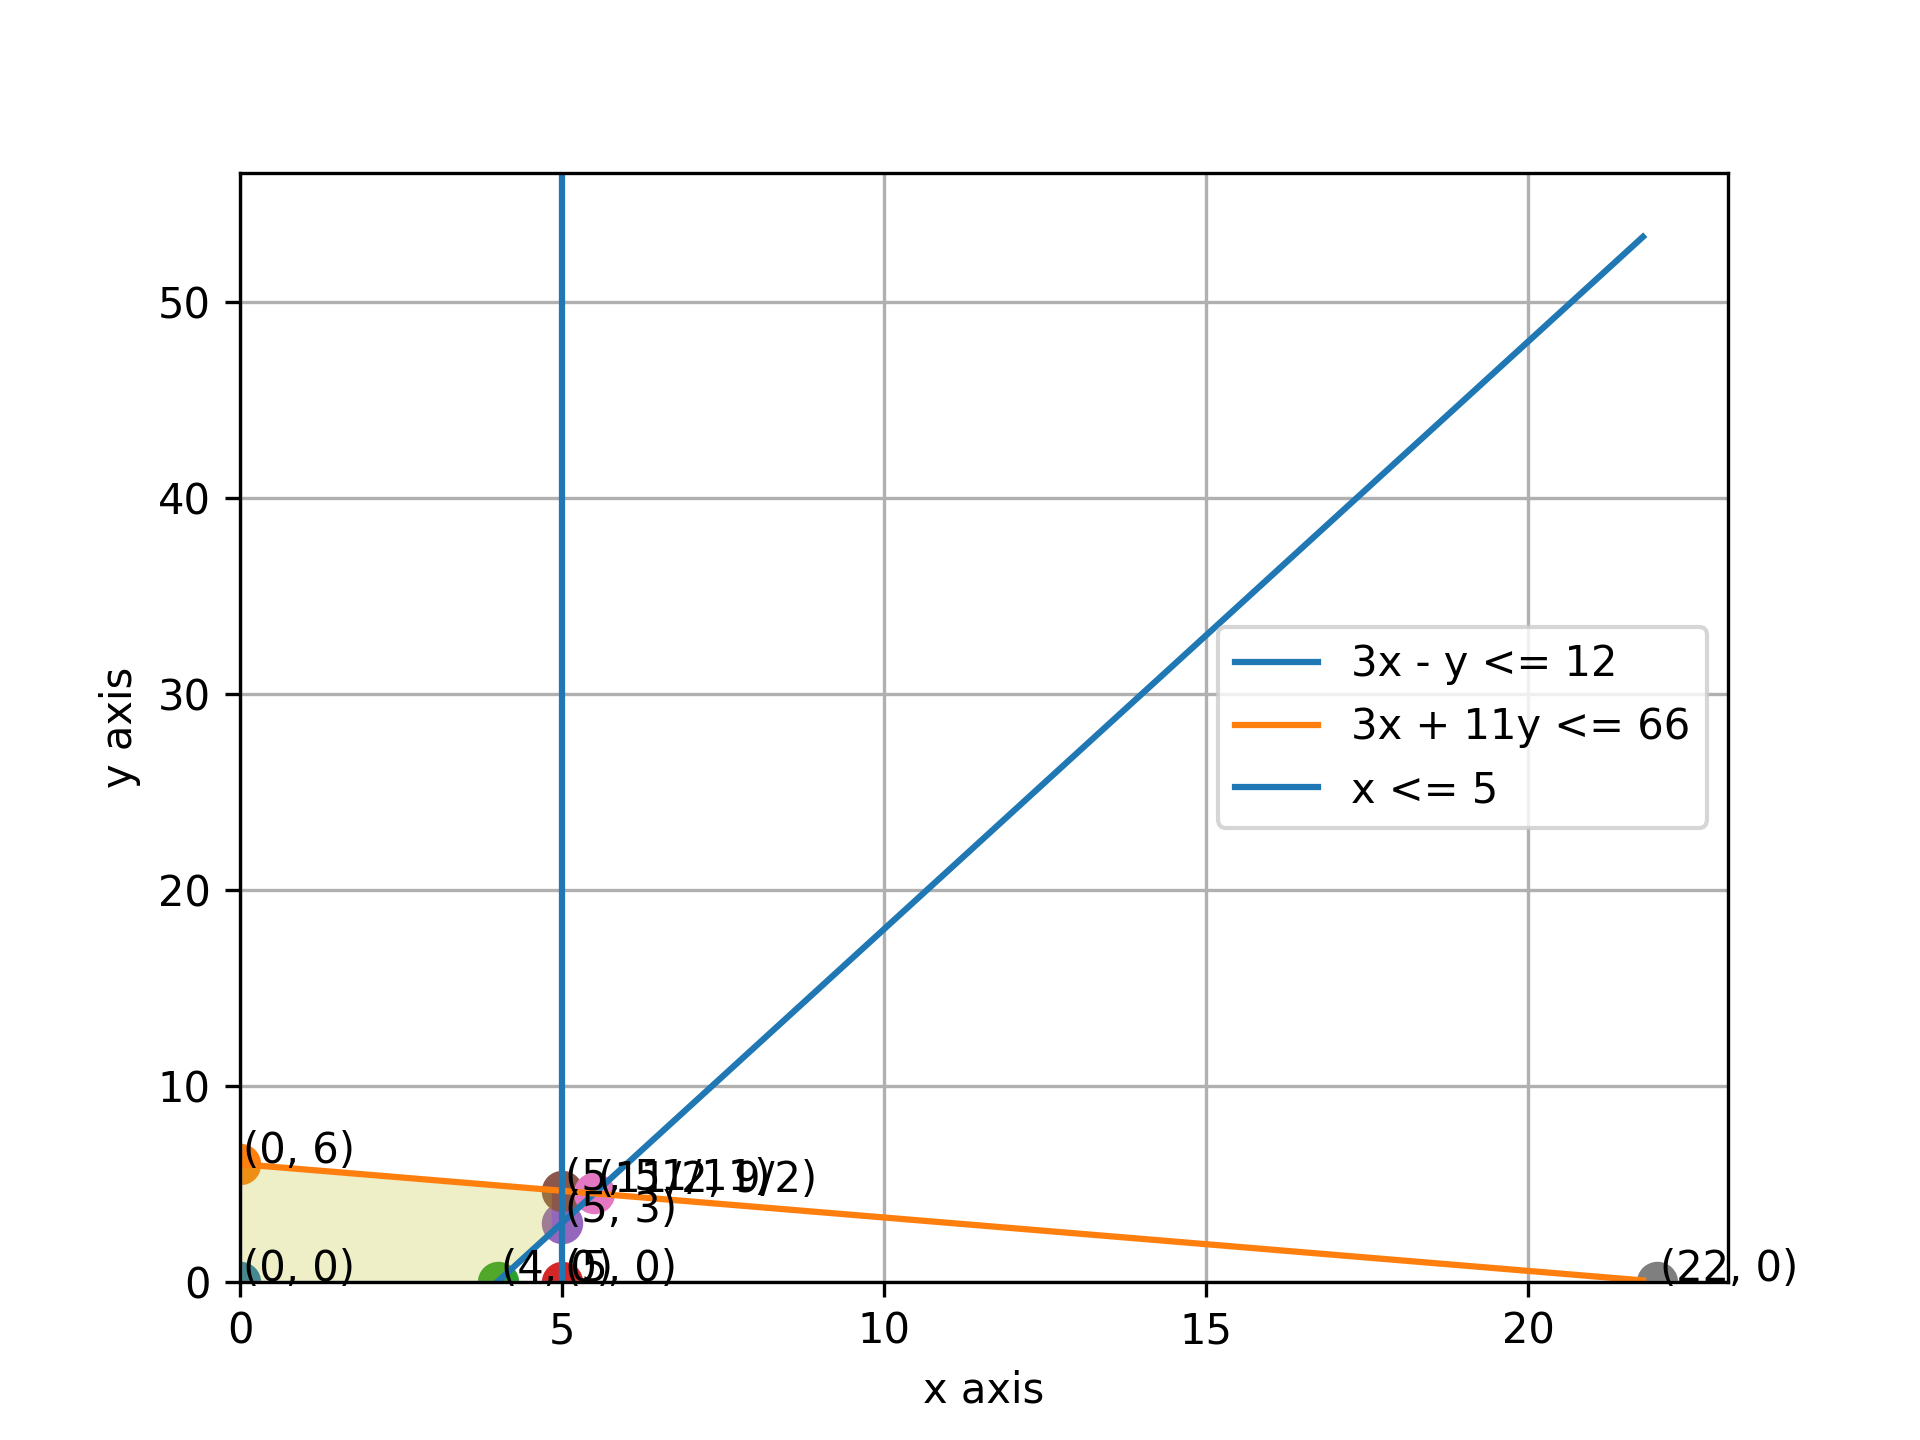
\includegraphics[width=0.6\textwidth]{outputs/ipp4/graph2.png}
\end{center}
\begin{align*}
Z=369\end{align*}
\begin{align*}
x=5\end{align*}
\begin{align*}
y=51\end{align*}
\begin{align*}
\text{Maximize} \quad & 3x + 4y\\
\text{subject to} \quad
& 3x - y\le12\\
& 3x + 11y\le66\\
& x\ge6\\
& x\ge0,\; y\ge0\end{align*}
\begin{align*}
3x - y=12\end{align*}
\begin{align*}
3x + 11y=66\end{align*}
Gauss Elimination:\\
Echelon Form:\\
\begin{align*}
\left(
\begin{array}{cc|c}
3 & -1 & 12\\
3 & 11 & 66\\
\end{array}
\right)_{2\times 3}
\end{align*}
\begin{align*}
\left(
\begin{array}{cc|c}
3 & -1 & 12\\
0 & 12 & 54\\
\end{array}
\right)_{2\times 3}
\end{align*}
\begin{align*}
\left(
\begin{array}{cc|c}
3 & -1 & 12\\
0 & 12 & 54\\
\end{array}
\right)_{2\times 3}
\end{align*}
\begin{align*}
x=\frac{11}{2}\end{align*}
\begin{align*}
y=\frac{9}{2}\end{align*}
\begin{align*}
3x - y=12\end{align*}
\begin{align*}
x=6\end{align*}
Gauss Elimination:\\
Echelon Form:\\
\begin{align*}
\left(
\begin{array}{cc|c}
3 & -1 & 12\\
1 & 0 & 6\\
\end{array}
\right)_{2\times 3}
\end{align*}
\begin{align*}
\left(
\begin{array}{cc|c}
3 & -1 & 12\\
0 & \frac{1}{3} & 2\\
\end{array}
\right)_{2\times 3}
\end{align*}
\begin{align*}
\left(
\begin{array}{cc|c}
3 & -1 & 12\\
0 & \frac{1}{3} & 2\\
\end{array}
\right)_{2\times 3}
\end{align*}
\begin{align*}
x=6\end{align*}
\begin{align*}
y=6\end{align*}
\begin{align*}
3x + 11y=66\end{align*}
\begin{align*}
x=6\end{align*}
Gauss Elimination:\\
Echelon Form:\\
\begin{align*}
\left(
\begin{array}{cc|c}
3 & 11 & 66\\
1 & 0 & 6\\
\end{array}
\right)_{2\times 3}
\end{align*}
\begin{align*}
\left(
\begin{array}{cc|c}
3 & 11 & 66\\
0 & -\frac{11}{3} & -16\\
\end{array}
\right)_{2\times 3}
\end{align*}
\begin{align*}
\left(
\begin{array}{cc|c}
3 & 11 & 66\\
0 & -\frac{11}{3} & -16\\
\end{array}
\right)_{2\times 3}
\end{align*}
\begin{align*}
x=6\end{align*}
\begin{align*}
y=\frac{48}{11}\end{align*}
\begin{center}
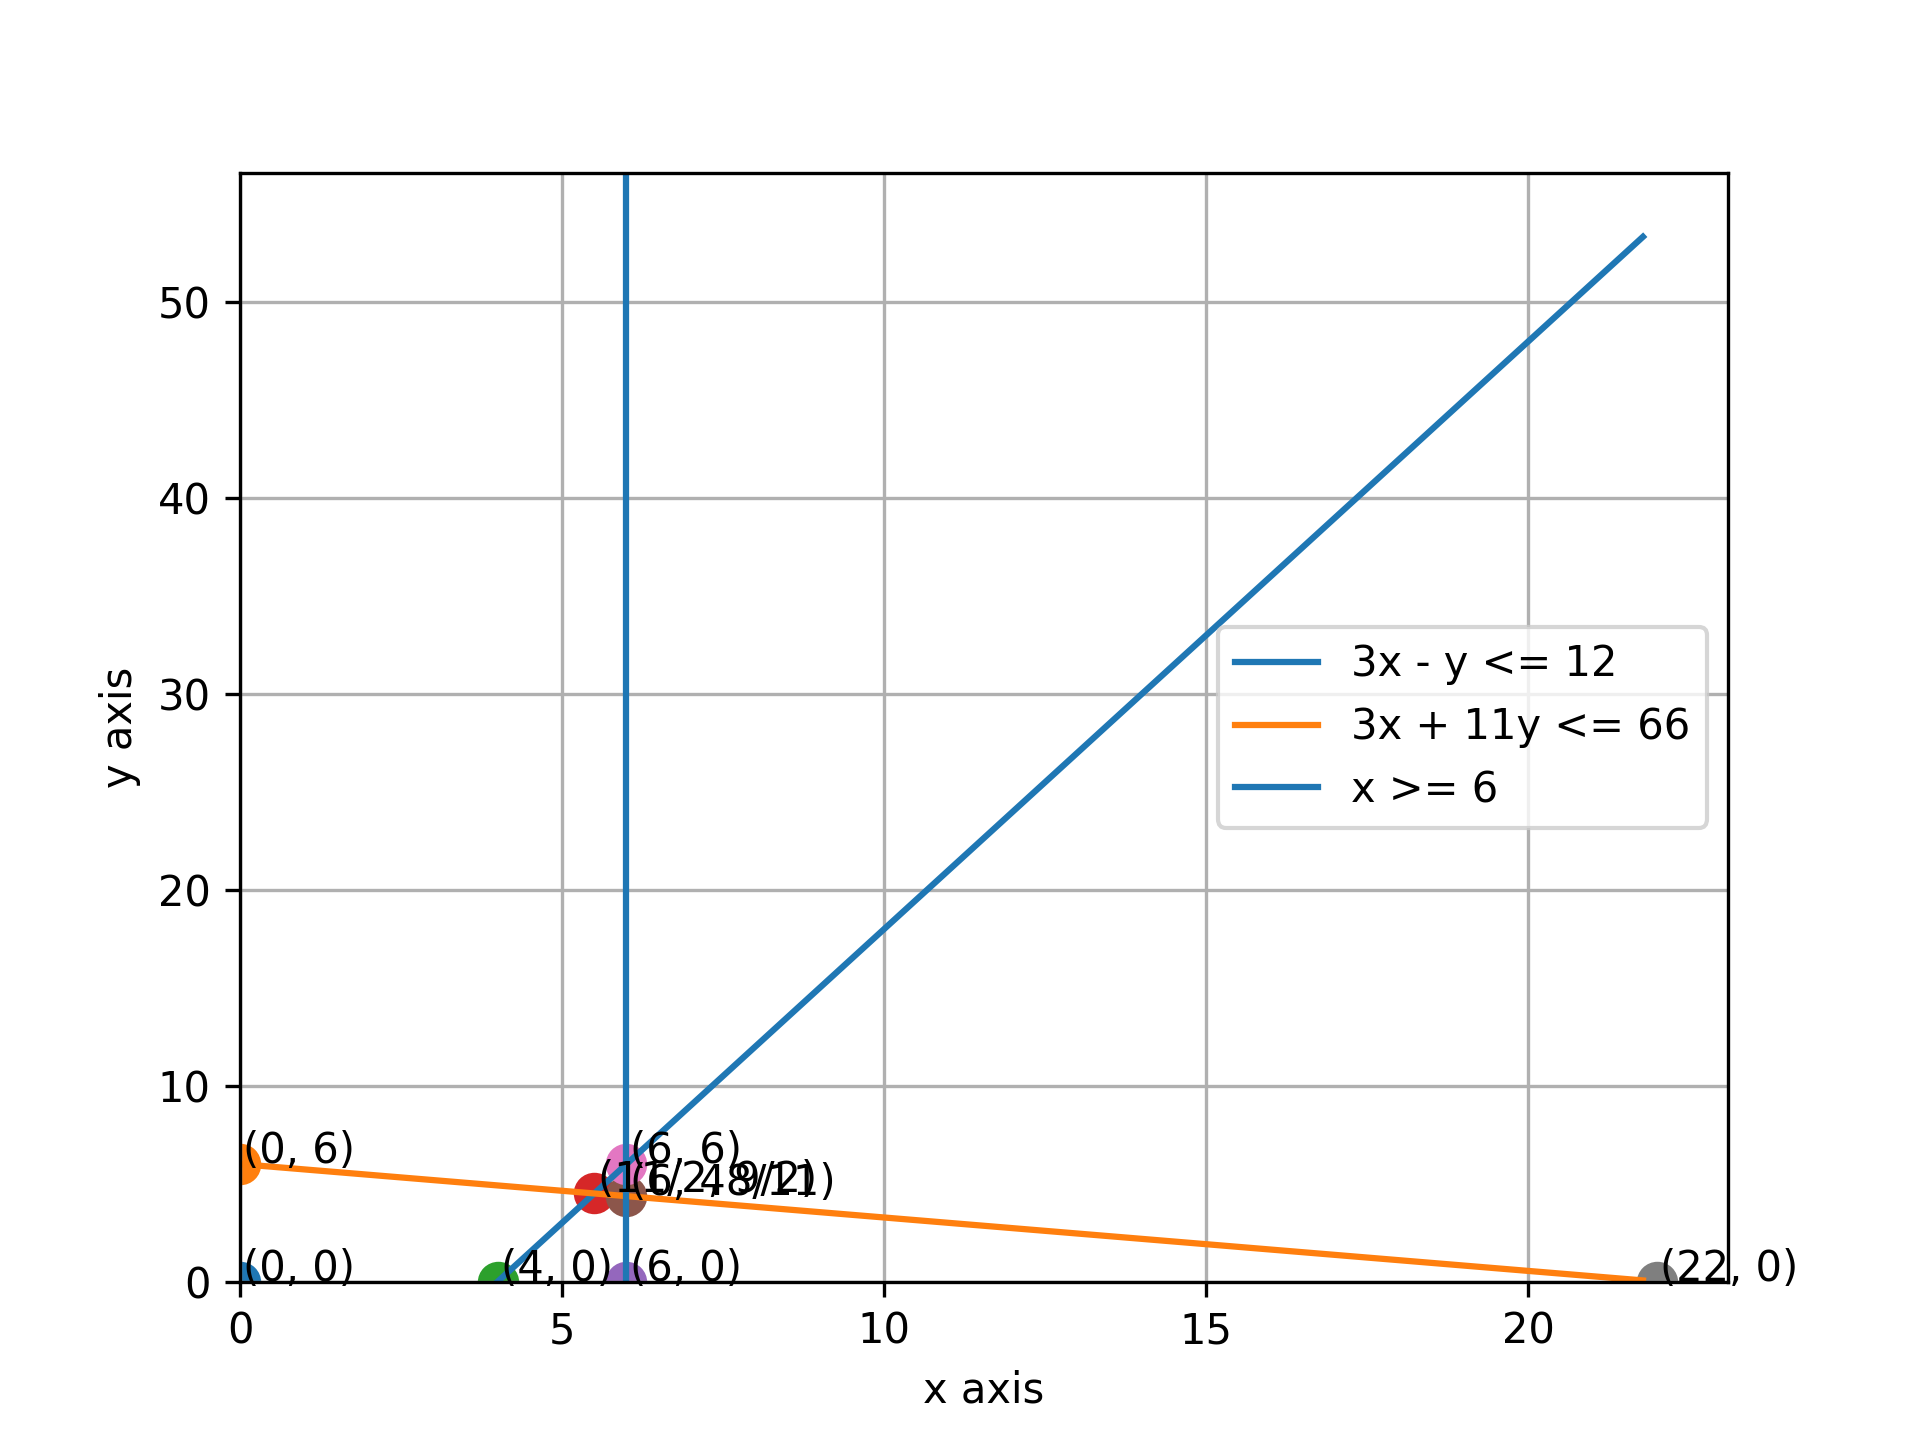
\includegraphics[width=0.6\textwidth]{outputs/ipp4/graph3.png}
\end{center}
Infeasible Solution\\
\begin{align*}
\text{Maximize} \quad & 3x + 4y\\
\text{subject to} \quad
& 3x - y\le12\\
& 3x + 11y\le66\\
& x\le5\\
& y\le4\\
& x\ge0,\; y\ge0\end{align*}
\begin{align*}
3x - y=12\end{align*}
\begin{align*}
3x + 11y=66\end{align*}
Gauss Elimination:\\
Echelon Form:\\
\begin{align*}
\left(
\begin{array}{cc|c}
3 & -1 & 12\\
3 & 11 & 66\\
\end{array}
\right)_{2\times 3}
\end{align*}
\begin{align*}
\left(
\begin{array}{cc|c}
3 & -1 & 12\\
0 & 12 & 54\\
\end{array}
\right)_{2\times 3}
\end{align*}
\begin{align*}
\left(
\begin{array}{cc|c}
3 & -1 & 12\\
0 & 12 & 54\\
\end{array}
\right)_{2\times 3}
\end{align*}
\begin{align*}
x=\frac{11}{2}\end{align*}
\begin{align*}
y=\frac{9}{2}\end{align*}
\begin{align*}
3x - y=12\end{align*}
\begin{align*}
x=5\end{align*}
Gauss Elimination:\\
Echelon Form:\\
\begin{align*}
\left(
\begin{array}{cc|c}
3 & -1 & 12\\
1 & 0 & 5\\
\end{array}
\right)_{2\times 3}
\end{align*}
\begin{align*}
\left(
\begin{array}{cc|c}
3 & -1 & 12\\
0 & \frac{1}{3} & 1\\
\end{array}
\right)_{2\times 3}
\end{align*}
\begin{align*}
\left(
\begin{array}{cc|c}
3 & -1 & 12\\
0 & \frac{1}{3} & 1\\
\end{array}
\right)_{2\times 3}
\end{align*}
\begin{align*}
x=5\end{align*}
\begin{align*}
y=3\end{align*}
\begin{align*}
3x - y=12\end{align*}
\begin{align*}
y=4\end{align*}
Gauss Elimination:\\
Echelon Form:\\
\begin{align*}
\left(
\begin{array}{cc|c}
3 & -1 & 12\\
0 & 1 & 4\\
\end{array}
\right)_{2\times 3}
\end{align*}
\begin{align*}
\left(
\begin{array}{cc|c}
3 & -1 & 12\\
0 & 1 & 4\\
\end{array}
\right)_{2\times 3}
\end{align*}
\begin{align*}
\left(
\begin{array}{cc|c}
3 & -1 & 12\\
0 & 1 & 4\\
\end{array}
\right)_{2\times 3}
\end{align*}
\begin{align*}
x=\frac{16}{3}\end{align*}
\begin{align*}
y=4\end{align*}
\begin{align*}
3x + 11y=66\end{align*}
\begin{align*}
x=5\end{align*}
Gauss Elimination:\\
Echelon Form:\\
\begin{align*}
\left(
\begin{array}{cc|c}
3 & 11 & 66\\
1 & 0 & 5\\
\end{array}
\right)_{2\times 3}
\end{align*}
\begin{align*}
\left(
\begin{array}{cc|c}
3 & 11 & 66\\
0 & -\frac{11}{3} & -17\\
\end{array}
\right)_{2\times 3}
\end{align*}
\begin{align*}
\left(
\begin{array}{cc|c}
3 & 11 & 66\\
0 & -\frac{11}{3} & -17\\
\end{array}
\right)_{2\times 3}
\end{align*}
\begin{align*}
x=5\end{align*}
\begin{align*}
y=\frac{51}{11}\end{align*}
\begin{align*}
3x + 11y=66\end{align*}
\begin{align*}
y=4\end{align*}
Gauss Elimination:\\
Echelon Form:\\
\begin{align*}
\left(
\begin{array}{cc|c}
3 & 11 & 66\\
0 & 1 & 4\\
\end{array}
\right)_{2\times 3}
\end{align*}
\begin{align*}
\left(
\begin{array}{cc|c}
3 & 11 & 66\\
0 & 1 & 4\\
\end{array}
\right)_{2\times 3}
\end{align*}
\begin{align*}
\left(
\begin{array}{cc|c}
3 & 11 & 66\\
0 & 1 & 4\\
\end{array}
\right)_{2\times 3}
\end{align*}
\begin{align*}
x=\frac{22}{3}\end{align*}
\begin{align*}
y=4\end{align*}
\begin{align*}
x=5\end{align*}
\begin{align*}
y=4\end{align*}
Gauss Elimination:\\
Echelon Form:\\
\begin{align*}
\left(
\begin{array}{cc|c}
1 & 0 & 5\\
0 & 1 & 4\\
\end{array}
\right)_{2\times 3}
\end{align*}
\begin{align*}
\left(
\begin{array}{cc|c}
1 & 0 & 5\\
0 & 1 & 4\\
\end{array}
\right)_{2\times 3}
\end{align*}
\begin{align*}
\left(
\begin{array}{cc|c}
1 & 0 & 5\\
0 & 1 & 4\\
\end{array}
\right)_{2\times 3}
\end{align*}
\begin{align*}
x=5\end{align*}
\begin{align*}
y=4\end{align*}
\begin{center}
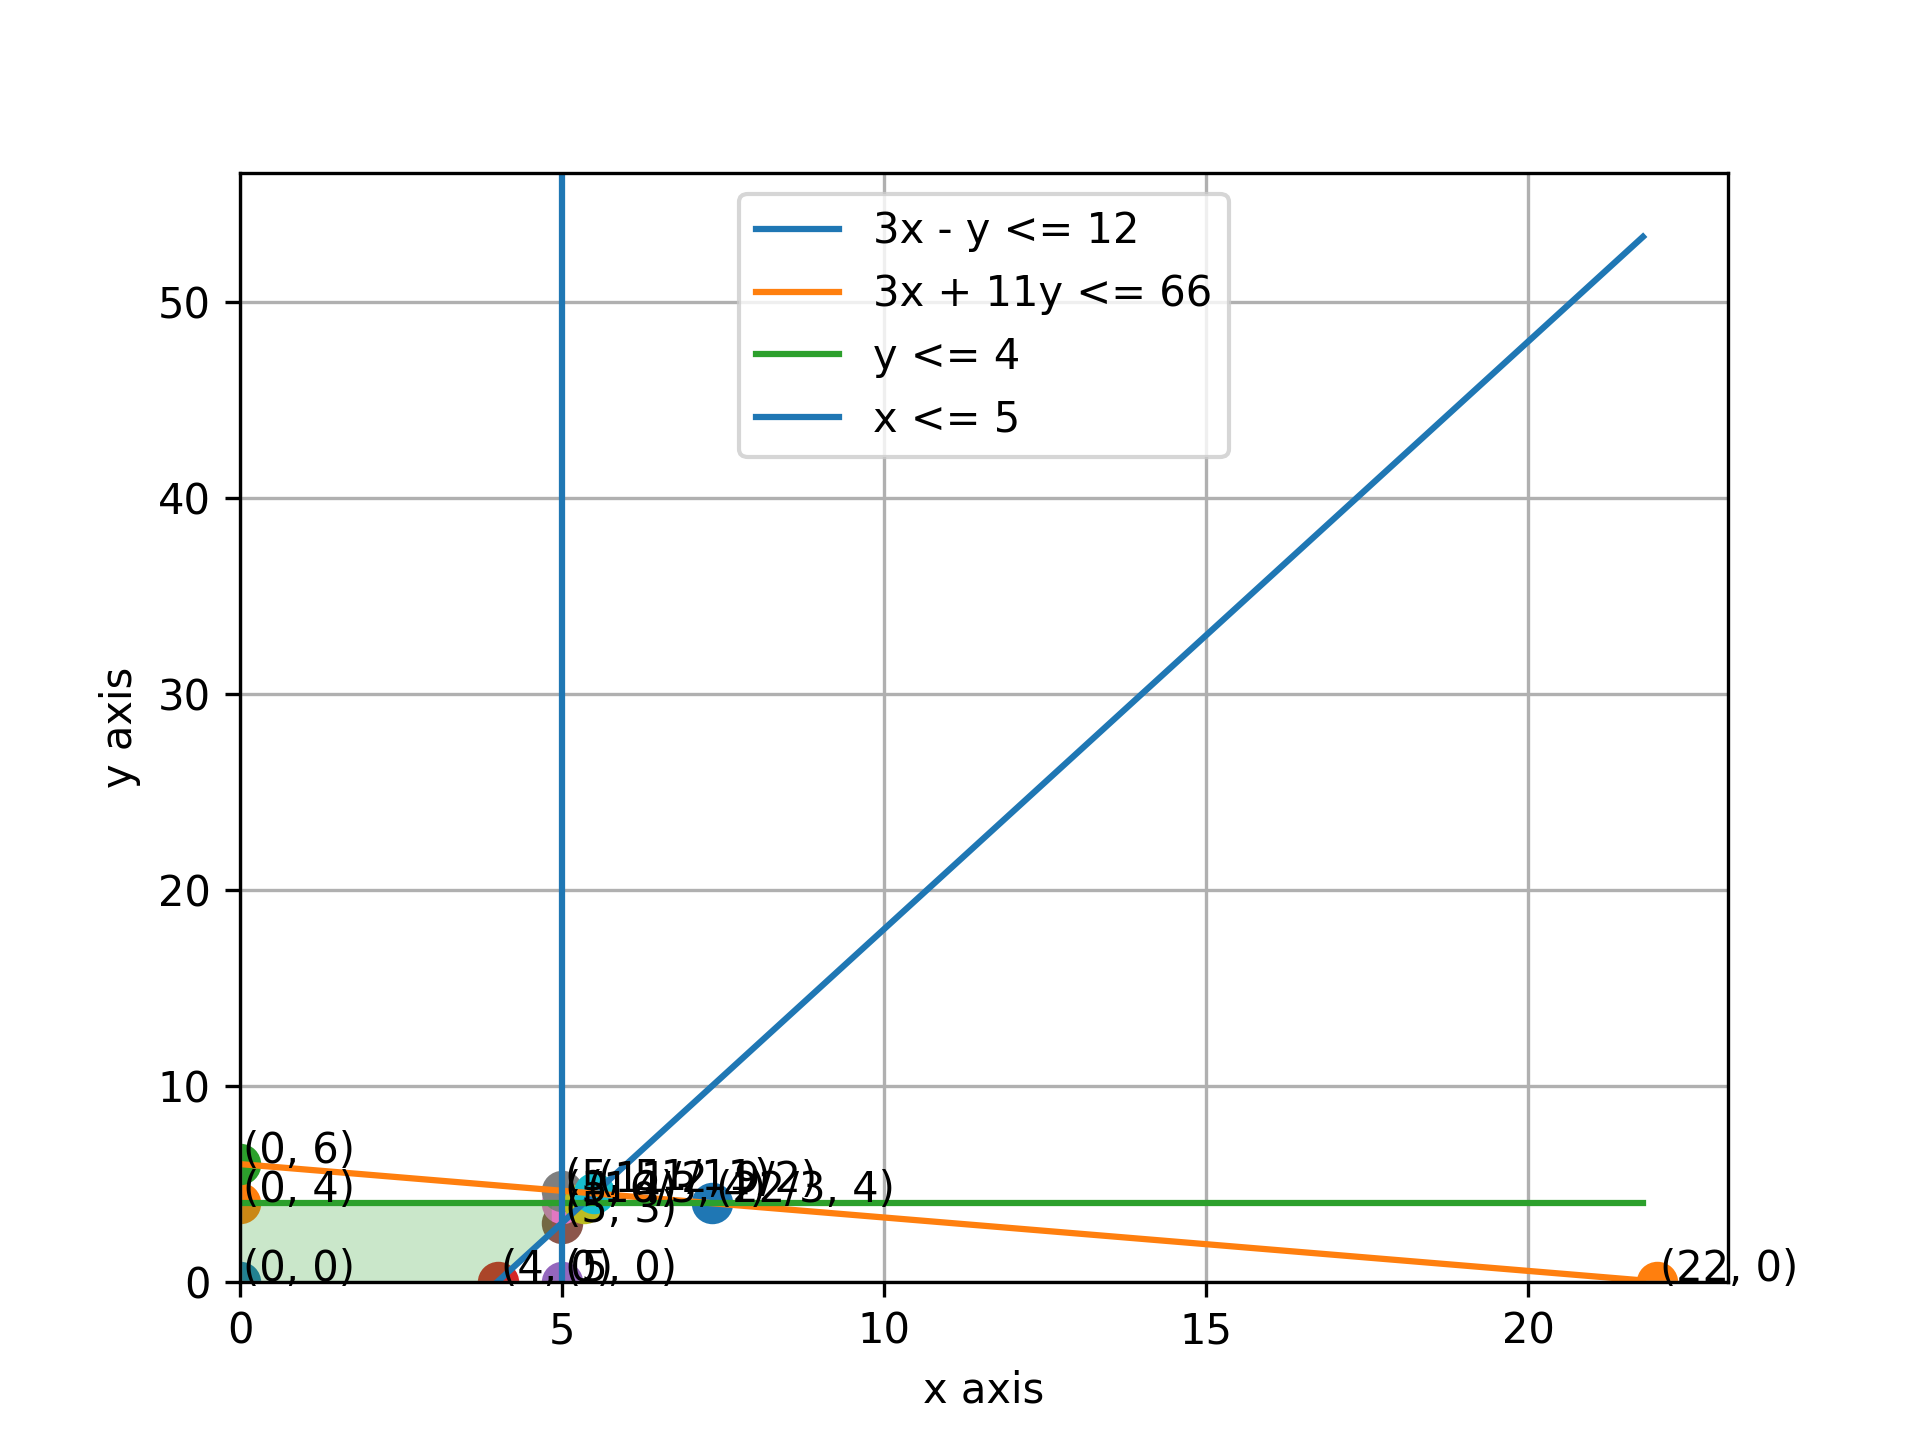
\includegraphics[width=0.6\textwidth]{outputs/ipp4/graph4.png}
\end{center}
\begin{align*}
Z=31\end{align*}
\begin{align*}
x=5\end{align*}
\begin{align*}
y=4\end{align*}
\begin{align*}
\text{Maximize} \quad & 3x + 4y\\
\text{subject to} \quad
& 3x - y\le12\\
& 3x + 11y\le66\\
& x\le5\\
& y\ge5\\
& x\ge0,\; y\ge0\end{align*}
\begin{align*}
3x - y=12\end{align*}
\begin{align*}
3x + 11y=66\end{align*}
Gauss Elimination:\\
Echelon Form:\\
\begin{align*}
\left(
\begin{array}{cc|c}
3 & -1 & 12\\
3 & 11 & 66\\
\end{array}
\right)_{2\times 3}
\end{align*}
\begin{align*}
\left(
\begin{array}{cc|c}
3 & -1 & 12\\
0 & 12 & 54\\
\end{array}
\right)_{2\times 3}
\end{align*}
\begin{align*}
\left(
\begin{array}{cc|c}
3 & -1 & 12\\
0 & 12 & 54\\
\end{array}
\right)_{2\times 3}
\end{align*}
\begin{align*}
x=\frac{11}{2}\end{align*}
\begin{align*}
y=\frac{9}{2}\end{align*}
\begin{align*}
3x - y=12\end{align*}
\begin{align*}
x=5\end{align*}
Gauss Elimination:\\
Echelon Form:\\
\begin{align*}
\left(
\begin{array}{cc|c}
3 & -1 & 12\\
1 & 0 & 5\\
\end{array}
\right)_{2\times 3}
\end{align*}
\begin{align*}
\left(
\begin{array}{cc|c}
3 & -1 & 12\\
0 & \frac{1}{3} & 1\\
\end{array}
\right)_{2\times 3}
\end{align*}
\begin{align*}
\left(
\begin{array}{cc|c}
3 & -1 & 12\\
0 & \frac{1}{3} & 1\\
\end{array}
\right)_{2\times 3}
\end{align*}
\begin{align*}
x=5\end{align*}
\begin{align*}
y=3\end{align*}
\begin{align*}
3x - y=12\end{align*}
\begin{align*}
y=5\end{align*}
Gauss Elimination:\\
Echelon Form:\\
\begin{align*}
\left(
\begin{array}{cc|c}
3 & -1 & 12\\
0 & 1 & 5\\
\end{array}
\right)_{2\times 3}
\end{align*}
\begin{align*}
\left(
\begin{array}{cc|c}
3 & -1 & 12\\
0 & 1 & 5\\
\end{array}
\right)_{2\times 3}
\end{align*}
\begin{align*}
\left(
\begin{array}{cc|c}
3 & -1 & 12\\
0 & 1 & 5\\
\end{array}
\right)_{2\times 3}
\end{align*}
\begin{align*}
x=\frac{17}{3}\end{align*}
\begin{align*}
y=5\end{align*}
\begin{align*}
3x + 11y=66\end{align*}
\begin{align*}
x=5\end{align*}
Gauss Elimination:\\
Echelon Form:\\
\begin{align*}
\left(
\begin{array}{cc|c}
3 & 11 & 66\\
1 & 0 & 5\\
\end{array}
\right)_{2\times 3}
\end{align*}
\begin{align*}
\left(
\begin{array}{cc|c}
3 & 11 & 66\\
0 & -\frac{11}{3} & -17\\
\end{array}
\right)_{2\times 3}
\end{align*}
\begin{align*}
\left(
\begin{array}{cc|c}
3 & 11 & 66\\
0 & -\frac{11}{3} & -17\\
\end{array}
\right)_{2\times 3}
\end{align*}
\begin{align*}
x=5\end{align*}
\begin{align*}
y=\frac{51}{11}\end{align*}
\begin{align*}
3x + 11y=66\end{align*}
\begin{align*}
y=5\end{align*}
Gauss Elimination:\\
Echelon Form:\\
\begin{align*}
\left(
\begin{array}{cc|c}
3 & 11 & 66\\
0 & 1 & 5\\
\end{array}
\right)_{2\times 3}
\end{align*}
\begin{align*}
\left(
\begin{array}{cc|c}
3 & 11 & 66\\
0 & 1 & 5\\
\end{array}
\right)_{2\times 3}
\end{align*}
\begin{align*}
\left(
\begin{array}{cc|c}
3 & 11 & 66\\
0 & 1 & 5\\
\end{array}
\right)_{2\times 3}
\end{align*}
\begin{align*}
x=\frac{11}{3}\end{align*}
\begin{align*}
y=5\end{align*}
\begin{align*}
x=5\end{align*}
\begin{align*}
y=5\end{align*}
Gauss Elimination:\\
Echelon Form:\\
\begin{align*}
\left(
\begin{array}{cc|c}
1 & 0 & 5\\
0 & 1 & 5\\
\end{array}
\right)_{2\times 3}
\end{align*}
\begin{align*}
\left(
\begin{array}{cc|c}
1 & 0 & 5\\
0 & 1 & 5\\
\end{array}
\right)_{2\times 3}
\end{align*}
\begin{align*}
\left(
\begin{array}{cc|c}
1 & 0 & 5\\
0 & 1 & 5\\
\end{array}
\right)_{2\times 3}
\end{align*}
\begin{align*}
x=5\end{align*}
\begin{align*}
y=5\end{align*}
\begin{center}
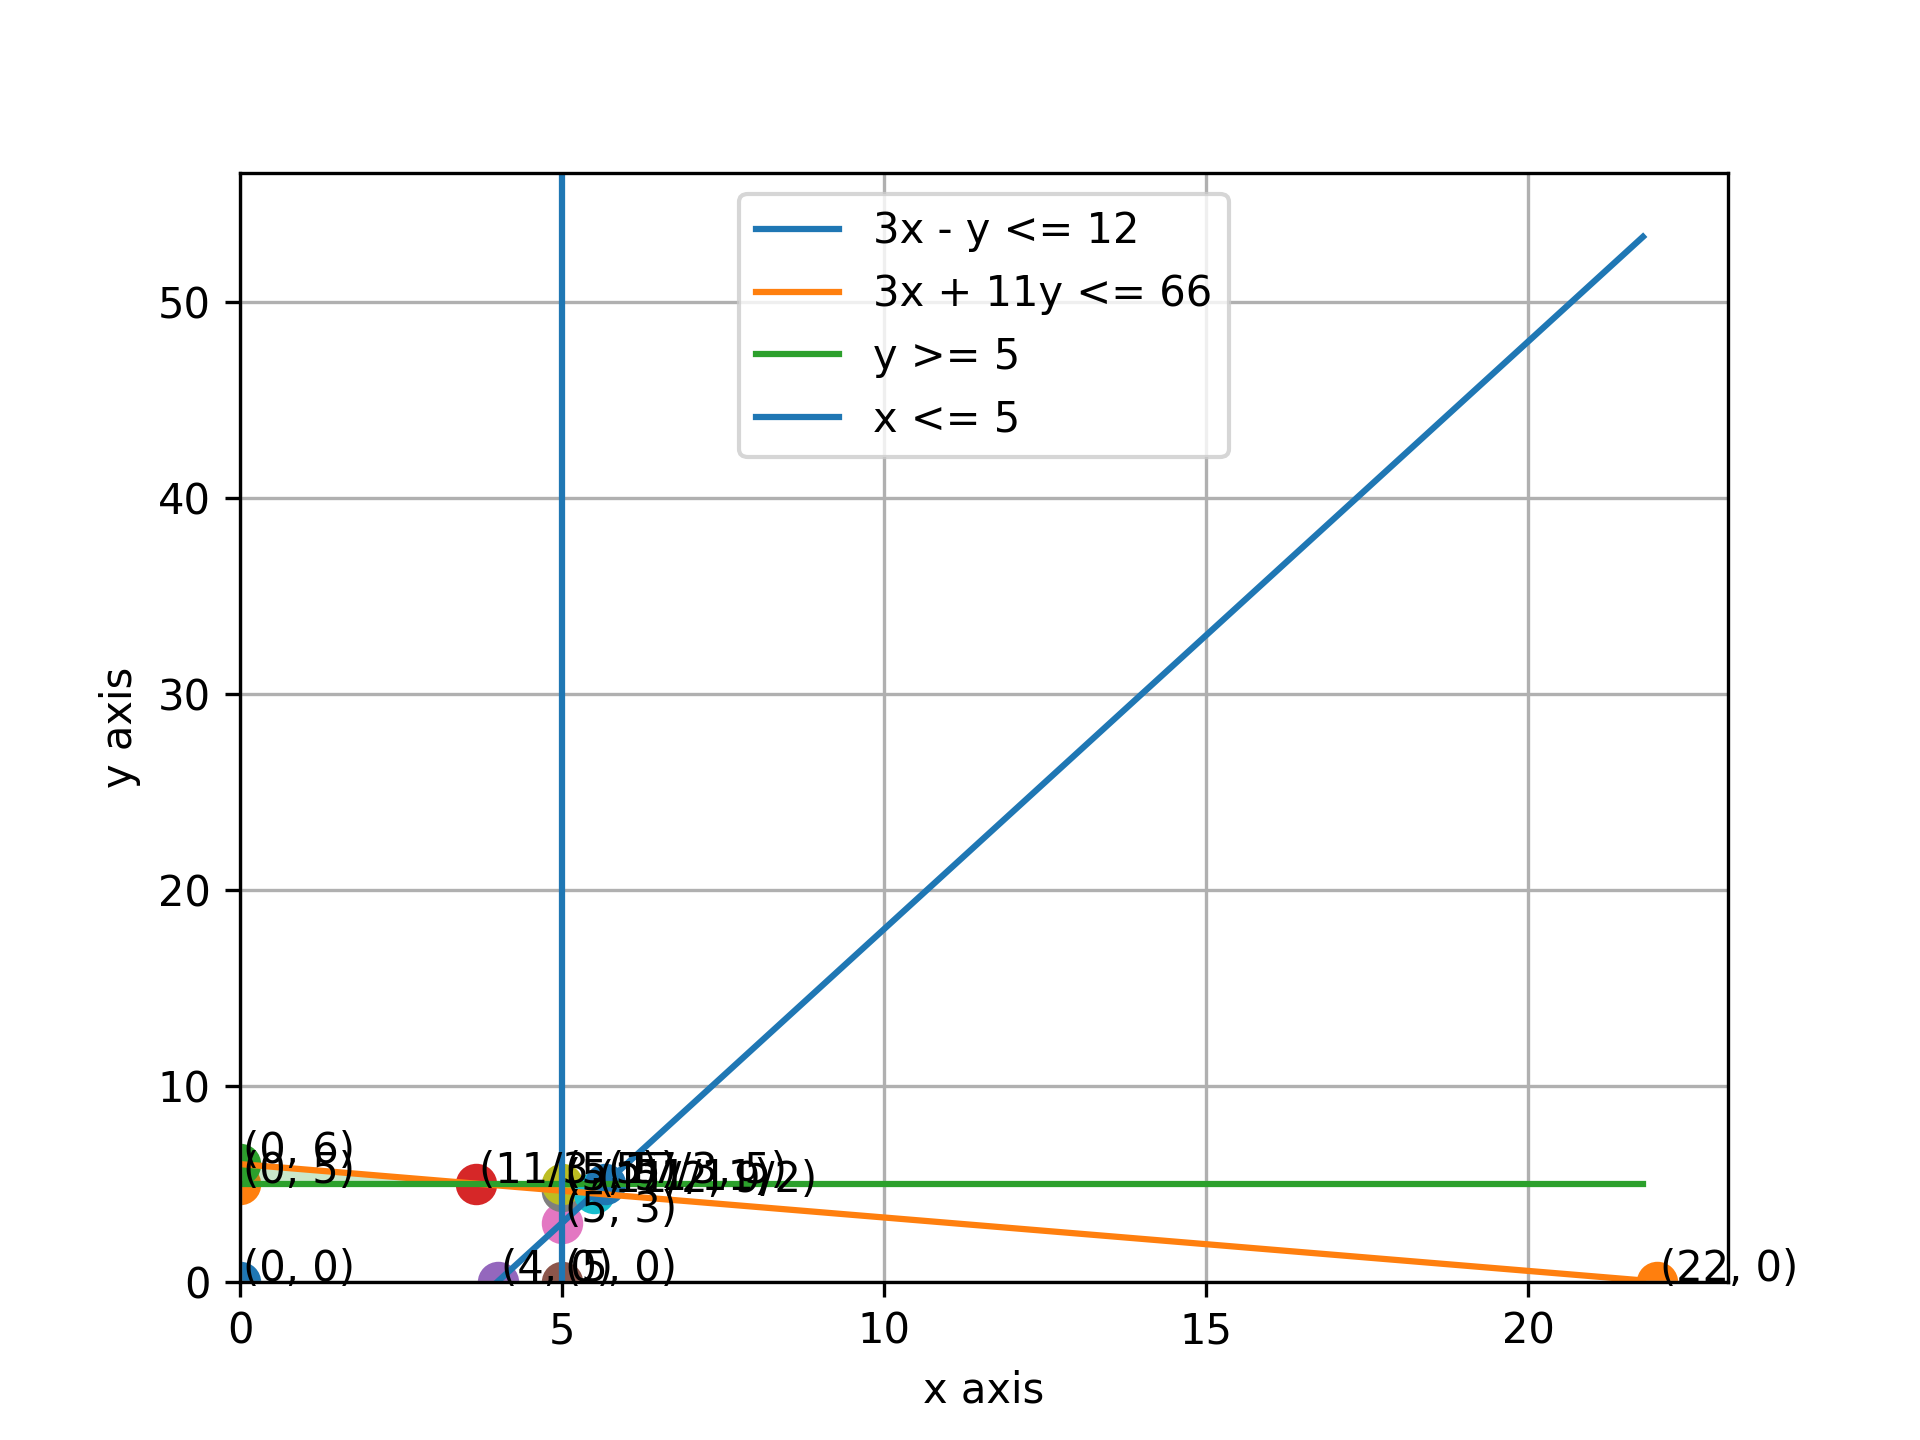
\includegraphics[width=0.6\textwidth]{outputs/ipp4/graph5.png}
\end{center}
\begin{align*}
Z=31\end{align*}
\begin{align*}
x=11\end{align*}
\begin{align*}
y=5\end{align*}
\begin{align*}
\text{Maximize} \quad & 3x + 4y\\
\text{subject to} \quad
& 3x - y\le12\\
& 3x + 11y\le66\\
& x\le5\\
& y\ge5\\
& x\le3\\
& x\ge0,\; y\ge0\end{align*}
\begin{align*}
3x - y=12\end{align*}
\begin{align*}
3x + 11y=66\end{align*}
Gauss Elimination:\\
Echelon Form:\\
\begin{align*}
\left(
\begin{array}{cc|c}
3 & -1 & 12\\
3 & 11 & 66\\
\end{array}
\right)_{2\times 3}
\end{align*}
\begin{align*}
\left(
\begin{array}{cc|c}
3 & -1 & 12\\
0 & 12 & 54\\
\end{array}
\right)_{2\times 3}
\end{align*}
\begin{align*}
\left(
\begin{array}{cc|c}
3 & -1 & 12\\
0 & 12 & 54\\
\end{array}
\right)_{2\times 3}
\end{align*}
\begin{align*}
x=\frac{11}{2}\end{align*}
\begin{align*}
y=\frac{9}{2}\end{align*}
\begin{align*}
3x - y=12\end{align*}
\begin{align*}
x=5\end{align*}
Gauss Elimination:\\
Echelon Form:\\
\begin{align*}
\left(
\begin{array}{cc|c}
3 & -1 & 12\\
1 & 0 & 5\\
\end{array}
\right)_{2\times 3}
\end{align*}
\begin{align*}
\left(
\begin{array}{cc|c}
3 & -1 & 12\\
0 & \frac{1}{3} & 1\\
\end{array}
\right)_{2\times 3}
\end{align*}
\begin{align*}
\left(
\begin{array}{cc|c}
3 & -1 & 12\\
0 & \frac{1}{3} & 1\\
\end{array}
\right)_{2\times 3}
\end{align*}
\begin{align*}
x=5\end{align*}
\begin{align*}
y=3\end{align*}
\begin{align*}
3x - y=12\end{align*}
\begin{align*}
y=5\end{align*}
Gauss Elimination:\\
Echelon Form:\\
\begin{align*}
\left(
\begin{array}{cc|c}
3 & -1 & 12\\
0 & 1 & 5\\
\end{array}
\right)_{2\times 3}
\end{align*}
\begin{align*}
\left(
\begin{array}{cc|c}
3 & -1 & 12\\
0 & 1 & 5\\
\end{array}
\right)_{2\times 3}
\end{align*}
\begin{align*}
\left(
\begin{array}{cc|c}
3 & -1 & 12\\
0 & 1 & 5\\
\end{array}
\right)_{2\times 3}
\end{align*}
\begin{align*}
x=\frac{17}{3}\end{align*}
\begin{align*}
y=5\end{align*}
\begin{align*}
3x - y=12\end{align*}
\begin{align*}
x=3\end{align*}
Gauss Elimination:\\
Echelon Form:\\
\begin{align*}
\left(
\begin{array}{cc|c}
3 & -1 & 12\\
1 & 0 & 3\\
\end{array}
\right)_{2\times 3}
\end{align*}
\begin{align*}
\left(
\begin{array}{cc|c}
3 & -1 & 12\\
0 & \frac{1}{3} & -1\\
\end{array}
\right)_{2\times 3}
\end{align*}
\begin{align*}
\left(
\begin{array}{cc|c}
3 & -1 & 12\\
0 & \frac{1}{3} & -1\\
\end{array}
\right)_{2\times 3}
\end{align*}
\begin{align*}
x=3\end{align*}
\begin{align*}
y=-3\end{align*}
\begin{align*}
3x + 11y=66\end{align*}
\begin{align*}
x=5\end{align*}
Gauss Elimination:\\
Echelon Form:\\
\begin{align*}
\left(
\begin{array}{cc|c}
3 & 11 & 66\\
1 & 0 & 5\\
\end{array}
\right)_{2\times 3}
\end{align*}
\begin{align*}
\left(
\begin{array}{cc|c}
3 & 11 & 66\\
0 & -\frac{11}{3} & -17\\
\end{array}
\right)_{2\times 3}
\end{align*}
\begin{align*}
\left(
\begin{array}{cc|c}
3 & 11 & 66\\
0 & -\frac{11}{3} & -17\\
\end{array}
\right)_{2\times 3}
\end{align*}
\begin{align*}
x=5\end{align*}
\begin{align*}
y=\frac{51}{11}\end{align*}
\begin{align*}
3x + 11y=66\end{align*}
\begin{align*}
y=5\end{align*}
Gauss Elimination:\\
Echelon Form:\\
\begin{align*}
\left(
\begin{array}{cc|c}
3 & 11 & 66\\
0 & 1 & 5\\
\end{array}
\right)_{2\times 3}
\end{align*}
\begin{align*}
\left(
\begin{array}{cc|c}
3 & 11 & 66\\
0 & 1 & 5\\
\end{array}
\right)_{2\times 3}
\end{align*}
\begin{align*}
\left(
\begin{array}{cc|c}
3 & 11 & 66\\
0 & 1 & 5\\
\end{array}
\right)_{2\times 3}
\end{align*}
\begin{align*}
x=\frac{11}{3}\end{align*}
\begin{align*}
y=5\end{align*}
\begin{align*}
3x + 11y=66\end{align*}
\begin{align*}
x=3\end{align*}
Gauss Elimination:\\
Echelon Form:\\
\begin{align*}
\left(
\begin{array}{cc|c}
3 & 11 & 66\\
1 & 0 & 3\\
\end{array}
\right)_{2\times 3}
\end{align*}
\begin{align*}
\left(
\begin{array}{cc|c}
3 & 11 & 66\\
0 & -\frac{11}{3} & -19\\
\end{array}
\right)_{2\times 3}
\end{align*}
\begin{align*}
\left(
\begin{array}{cc|c}
3 & 11 & 66\\
0 & -\frac{11}{3} & -19\\
\end{array}
\right)_{2\times 3}
\end{align*}
\begin{align*}
x=3\end{align*}
\begin{align*}
y=\frac{57}{11}\end{align*}
\begin{align*}
x=5\end{align*}
\begin{align*}
y=5\end{align*}
Gauss Elimination:\\
Echelon Form:\\
\begin{align*}
\left(
\begin{array}{cc|c}
1 & 0 & 5\\
0 & 1 & 5\\
\end{array}
\right)_{2\times 3}
\end{align*}
\begin{align*}
\left(
\begin{array}{cc|c}
1 & 0 & 5\\
0 & 1 & 5\\
\end{array}
\right)_{2\times 3}
\end{align*}
\begin{align*}
\left(
\begin{array}{cc|c}
1 & 0 & 5\\
0 & 1 & 5\\
\end{array}
\right)_{2\times 3}
\end{align*}
\begin{align*}
x=5\end{align*}
\begin{align*}
y=5\end{align*}
\begin{align*}
x=5\end{align*}
\begin{align*}
x=3\end{align*}
Gauss Elimination:\\
Echelon Form:\\
\begin{align*}
\left(
\begin{array}{c|c}
1 & 5\\
1 & 3\\
\end{array}
\right)_{2\times 2}
\end{align*}
\begin{align*}
\left(
\begin{array}{c|c}
1 & 5\\
0 & -2\\
\end{array}
\right)_{2\times 2}
\end{align*}
\begin{align*}
\left(
\begin{array}{c|c}
1 & 5\\
0 & -2\\
\end{array}
\right)_{2\times 2}
\end{align*}
No solution\\
\begin{align*}
y=5\end{align*}
\begin{align*}
x=3\end{align*}
Gauss Elimination:\\
Echelon Form:\\
\begin{align*}
\left(
\begin{array}{cc|c}
0 & 1 & 5\\
1 & 0 & 3\\
\end{array}
\right)_{2\times 3}
\end{align*}
\begin{align*}
\left(
\begin{array}{cc|c}
1 & 0 & 3\\
0 & 1 & 5\\
\end{array}
\right)_{2\times 3}
\end{align*}
\begin{align*}
\left(
\begin{array}{cc|c}
1 & 0 & 3\\
0 & 1 & 5\\
\end{array}
\right)_{2\times 3}
\end{align*}
\begin{align*}
x=3\end{align*}
\begin{align*}
y=5\end{align*}
\begin{center}
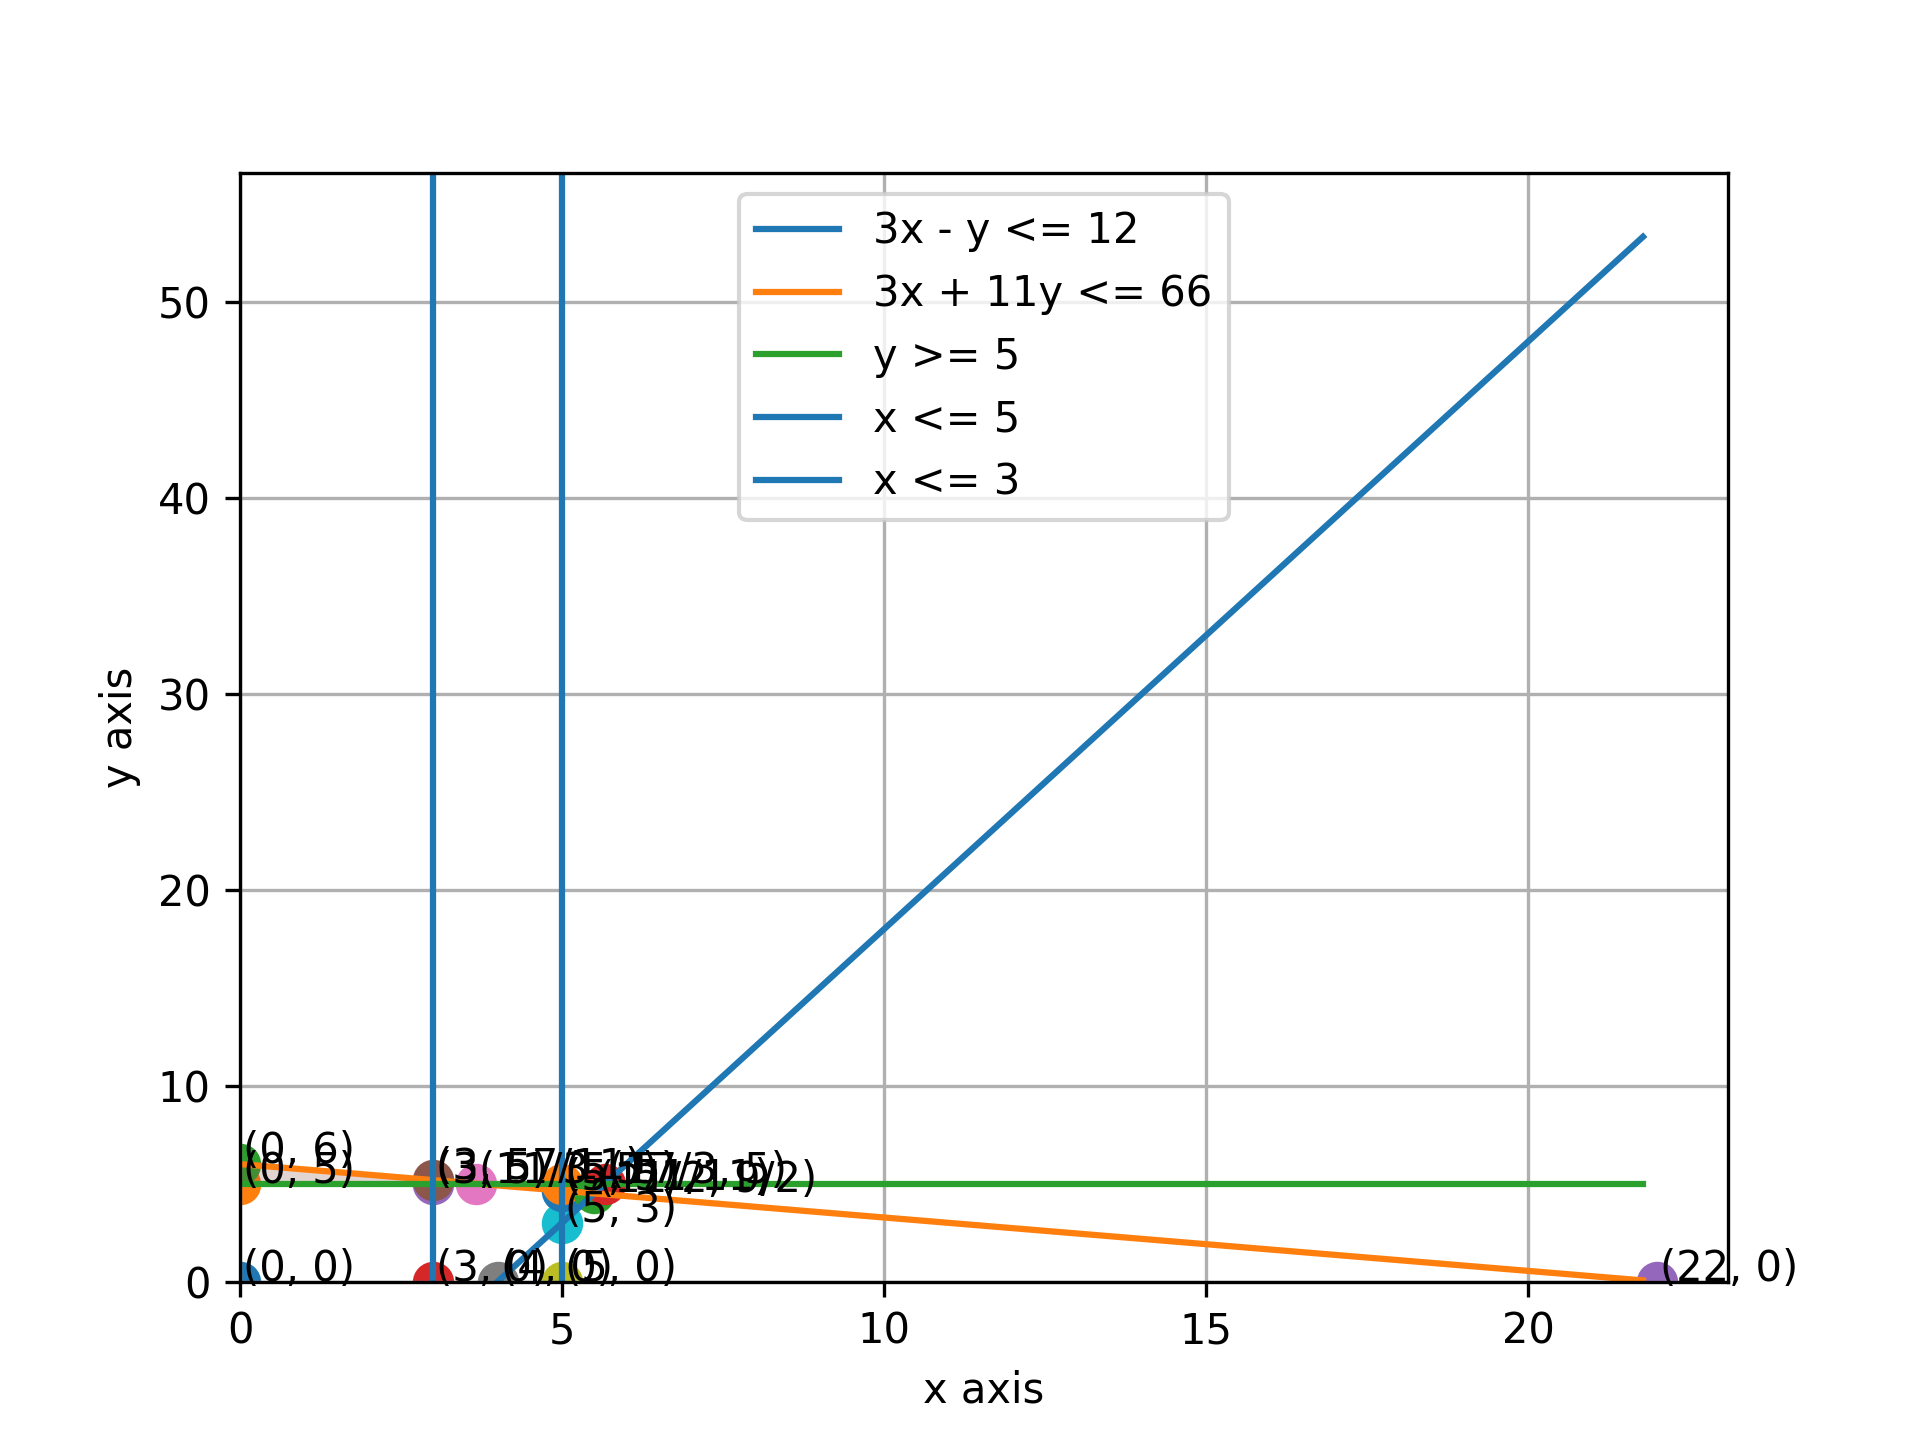
\includegraphics[width=0.6\textwidth]{outputs/ipp4/graph6.png}
\end{center}
\begin{align*}
Z=327\end{align*}
\begin{align*}
x=3\end{align*}
\begin{align*}
y=57\end{align*}
\begin{align*}
\text{Maximize} \quad & 3x + 4y\\
\text{subject to} \quad
& 3x - y\le12\\
& 3x + 11y\le66\\
& x\le5\\
& y\ge5\\
& x\ge4\\
& x\ge0,\; y\ge0\end{align*}
\begin{align*}
3x - y=12\end{align*}
\begin{align*}
3x + 11y=66\end{align*}
Gauss Elimination:\\
Echelon Form:\\
\begin{align*}
\left(
\begin{array}{cc|c}
3 & -1 & 12\\
3 & 11 & 66\\
\end{array}
\right)_{2\times 3}
\end{align*}
\begin{align*}
\left(
\begin{array}{cc|c}
3 & -1 & 12\\
0 & 12 & 54\\
\end{array}
\right)_{2\times 3}
\end{align*}
\begin{align*}
\left(
\begin{array}{cc|c}
3 & -1 & 12\\
0 & 12 & 54\\
\end{array}
\right)_{2\times 3}
\end{align*}
\begin{align*}
x=\frac{11}{2}\end{align*}
\begin{align*}
y=\frac{9}{2}\end{align*}
\begin{align*}
3x - y=12\end{align*}
\begin{align*}
x=5\end{align*}
Gauss Elimination:\\
Echelon Form:\\
\begin{align*}
\left(
\begin{array}{cc|c}
3 & -1 & 12\\
1 & 0 & 5\\
\end{array}
\right)_{2\times 3}
\end{align*}
\begin{align*}
\left(
\begin{array}{cc|c}
3 & -1 & 12\\
0 & \frac{1}{3} & 1\\
\end{array}
\right)_{2\times 3}
\end{align*}
\begin{align*}
\left(
\begin{array}{cc|c}
3 & -1 & 12\\
0 & \frac{1}{3} & 1\\
\end{array}
\right)_{2\times 3}
\end{align*}
\begin{align*}
x=5\end{align*}
\begin{align*}
y=3\end{align*}
\begin{align*}
3x - y=12\end{align*}
\begin{align*}
y=5\end{align*}
Gauss Elimination:\\
Echelon Form:\\
\begin{align*}
\left(
\begin{array}{cc|c}
3 & -1 & 12\\
0 & 1 & 5\\
\end{array}
\right)_{2\times 3}
\end{align*}
\begin{align*}
\left(
\begin{array}{cc|c}
3 & -1 & 12\\
0 & 1 & 5\\
\end{array}
\right)_{2\times 3}
\end{align*}
\begin{align*}
\left(
\begin{array}{cc|c}
3 & -1 & 12\\
0 & 1 & 5\\
\end{array}
\right)_{2\times 3}
\end{align*}
\begin{align*}
x=\frac{17}{3}\end{align*}
\begin{align*}
y=5\end{align*}
\begin{align*}
3x - y=12\end{align*}
\begin{align*}
x=4\end{align*}
Gauss Elimination:\\
Echelon Form:\\
\begin{align*}
\left(
\begin{array}{cc|c}
3 & -1 & 12\\
1 & 0 & 4\\
\end{array}
\right)_{2\times 3}
\end{align*}
\begin{align*}
\left(
\begin{array}{cc|c}
3 & -1 & 12\\
0 & \frac{1}{3} & 0\\
\end{array}
\right)_{2\times 3}
\end{align*}
\begin{align*}
\left(
\begin{array}{cc|c}
3 & -1 & 12\\
0 & \frac{1}{3} & 0\\
\end{array}
\right)_{2\times 3}
\end{align*}
\begin{align*}
x=4\end{align*}
\begin{align*}
y=0\end{align*}
\begin{align*}
3x + 11y=66\end{align*}
\begin{align*}
x=5\end{align*}
Gauss Elimination:\\
Echelon Form:\\
\begin{align*}
\left(
\begin{array}{cc|c}
3 & 11 & 66\\
1 & 0 & 5\\
\end{array}
\right)_{2\times 3}
\end{align*}
\begin{align*}
\left(
\begin{array}{cc|c}
3 & 11 & 66\\
0 & -\frac{11}{3} & -17\\
\end{array}
\right)_{2\times 3}
\end{align*}
\begin{align*}
\left(
\begin{array}{cc|c}
3 & 11 & 66\\
0 & -\frac{11}{3} & -17\\
\end{array}
\right)_{2\times 3}
\end{align*}
\begin{align*}
x=5\end{align*}
\begin{align*}
y=\frac{51}{11}\end{align*}
\begin{align*}
3x + 11y=66\end{align*}
\begin{align*}
y=5\end{align*}
Gauss Elimination:\\
Echelon Form:\\
\begin{align*}
\left(
\begin{array}{cc|c}
3 & 11 & 66\\
0 & 1 & 5\\
\end{array}
\right)_{2\times 3}
\end{align*}
\begin{align*}
\left(
\begin{array}{cc|c}
3 & 11 & 66\\
0 & 1 & 5\\
\end{array}
\right)_{2\times 3}
\end{align*}
\begin{align*}
\left(
\begin{array}{cc|c}
3 & 11 & 66\\
0 & 1 & 5\\
\end{array}
\right)_{2\times 3}
\end{align*}
\begin{align*}
x=\frac{11}{3}\end{align*}
\begin{align*}
y=5\end{align*}
\begin{align*}
3x + 11y=66\end{align*}
\begin{align*}
x=4\end{align*}
Gauss Elimination:\\
Echelon Form:\\
\begin{align*}
\left(
\begin{array}{cc|c}
3 & 11 & 66\\
1 & 0 & 4\\
\end{array}
\right)_{2\times 3}
\end{align*}
\begin{align*}
\left(
\begin{array}{cc|c}
3 & 11 & 66\\
0 & -\frac{11}{3} & -18\\
\end{array}
\right)_{2\times 3}
\end{align*}
\begin{align*}
\left(
\begin{array}{cc|c}
3 & 11 & 66\\
0 & -\frac{11}{3} & -18\\
\end{array}
\right)_{2\times 3}
\end{align*}
\begin{align*}
x=4\end{align*}
\begin{align*}
y=\frac{54}{11}\end{align*}
\begin{align*}
x=5\end{align*}
\begin{align*}
y=5\end{align*}
Gauss Elimination:\\
Echelon Form:\\
\begin{align*}
\left(
\begin{array}{cc|c}
1 & 0 & 5\\
0 & 1 & 5\\
\end{array}
\right)_{2\times 3}
\end{align*}
\begin{align*}
\left(
\begin{array}{cc|c}
1 & 0 & 5\\
0 & 1 & 5\\
\end{array}
\right)_{2\times 3}
\end{align*}
\begin{align*}
\left(
\begin{array}{cc|c}
1 & 0 & 5\\
0 & 1 & 5\\
\end{array}
\right)_{2\times 3}
\end{align*}
\begin{align*}
x=5\end{align*}
\begin{align*}
y=5\end{align*}
\begin{align*}
x=5\end{align*}
\begin{align*}
x=4\end{align*}
Gauss Elimination:\\
Echelon Form:\\
\begin{align*}
\left(
\begin{array}{c|c}
1 & 5\\
1 & 4\\
\end{array}
\right)_{2\times 2}
\end{align*}
\begin{align*}
\left(
\begin{array}{c|c}
1 & 5\\
0 & -1\\
\end{array}
\right)_{2\times 2}
\end{align*}
\begin{align*}
\left(
\begin{array}{c|c}
1 & 5\\
0 & -1\\
\end{array}
\right)_{2\times 2}
\end{align*}
No solution\\
\begin{align*}
y=5\end{align*}
\begin{align*}
x=4\end{align*}
Gauss Elimination:\\
Echelon Form:\\
\begin{align*}
\left(
\begin{array}{cc|c}
0 & 1 & 5\\
1 & 0 & 4\\
\end{array}
\right)_{2\times 3}
\end{align*}
\begin{align*}
\left(
\begin{array}{cc|c}
1 & 0 & 4\\
0 & 1 & 5\\
\end{array}
\right)_{2\times 3}
\end{align*}
\begin{align*}
\left(
\begin{array}{cc|c}
1 & 0 & 4\\
0 & 1 & 5\\
\end{array}
\right)_{2\times 3}
\end{align*}
\begin{align*}
x=4\end{align*}
\begin{align*}
y=5\end{align*}
\begin{center}
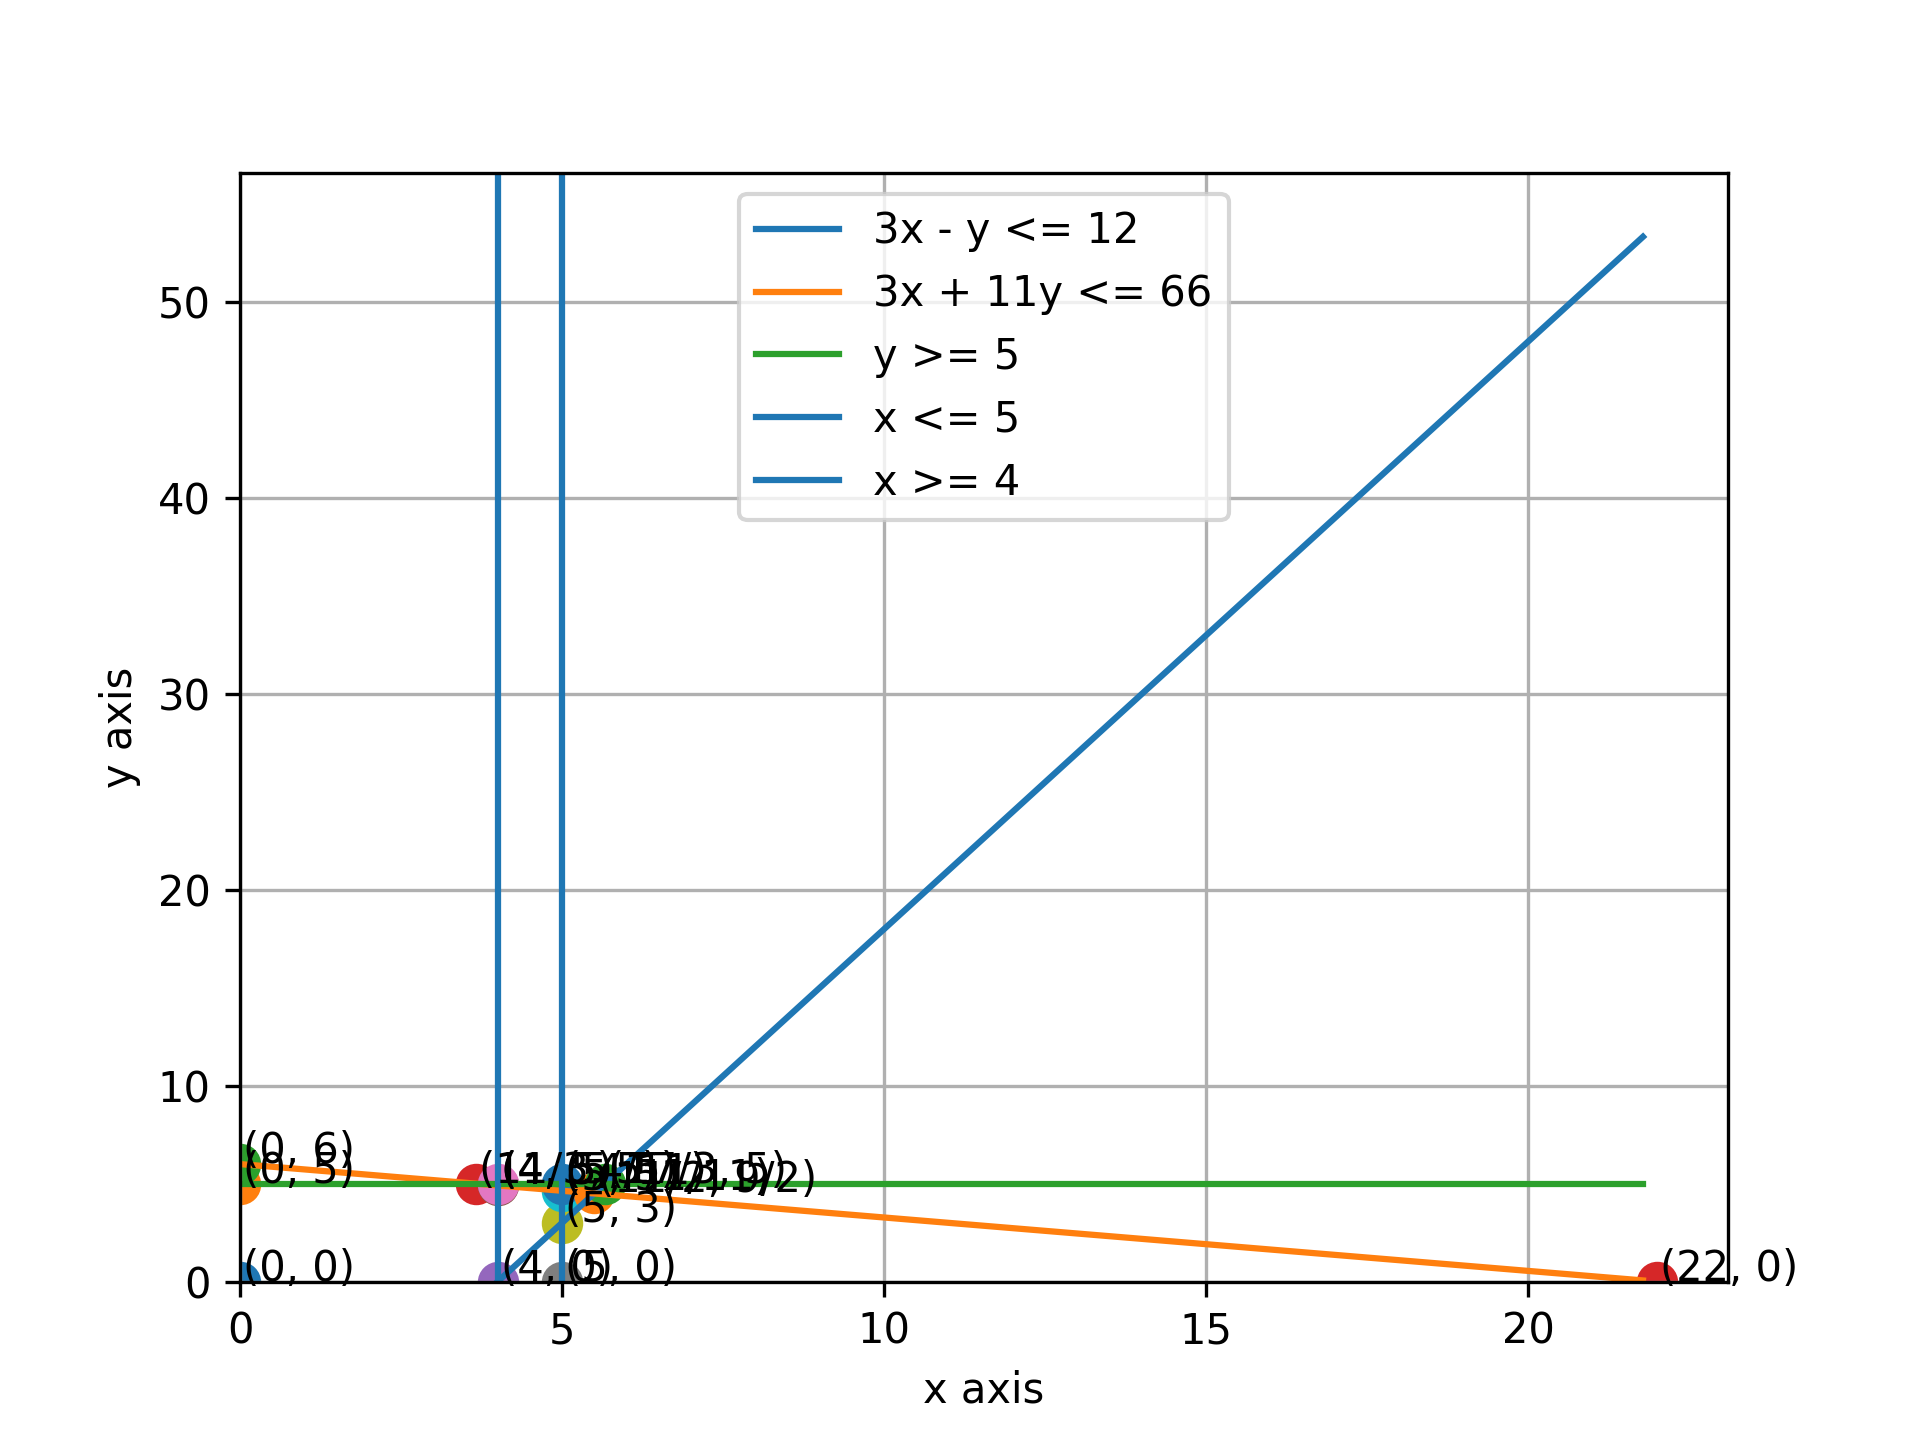
\includegraphics[width=0.6\textwidth]{outputs/ipp4/graph7.png}
\end{center}
Infeasible Solution\\
\begin{align*}
\text{Maximize} \quad & 3x + 4y\\
\text{subject to} \quad
& 3x - y\le12\\
& 3x + 11y\le66\\
& x\le5\\
& y\ge5\\
& x\le3\\
& y\le5\\
& x\ge0,\; y\ge0\end{align*}
\begin{align*}
3x - y=12\end{align*}
\begin{align*}
3x + 11y=66\end{align*}
Gauss Elimination:\\
Echelon Form:\\
\begin{align*}
\left(
\begin{array}{cc|c}
3 & -1 & 12\\
3 & 11 & 66\\
\end{array}
\right)_{2\times 3}
\end{align*}
\begin{align*}
\left(
\begin{array}{cc|c}
3 & -1 & 12\\
0 & 12 & 54\\
\end{array}
\right)_{2\times 3}
\end{align*}
\begin{align*}
\left(
\begin{array}{cc|c}
3 & -1 & 12\\
0 & 12 & 54\\
\end{array}
\right)_{2\times 3}
\end{align*}
\begin{align*}
x=\frac{11}{2}\end{align*}
\begin{align*}
y=\frac{9}{2}\end{align*}
\begin{align*}
3x - y=12\end{align*}
\begin{align*}
x=5\end{align*}
Gauss Elimination:\\
Echelon Form:\\
\begin{align*}
\left(
\begin{array}{cc|c}
3 & -1 & 12\\
1 & 0 & 5\\
\end{array}
\right)_{2\times 3}
\end{align*}
\begin{align*}
\left(
\begin{array}{cc|c}
3 & -1 & 12\\
0 & \frac{1}{3} & 1\\
\end{array}
\right)_{2\times 3}
\end{align*}
\begin{align*}
\left(
\begin{array}{cc|c}
3 & -1 & 12\\
0 & \frac{1}{3} & 1\\
\end{array}
\right)_{2\times 3}
\end{align*}
\begin{align*}
x=5\end{align*}
\begin{align*}
y=3\end{align*}
\begin{align*}
3x - y=12\end{align*}
\begin{align*}
y=5\end{align*}
Gauss Elimination:\\
Echelon Form:\\
\begin{align*}
\left(
\begin{array}{cc|c}
3 & -1 & 12\\
0 & 1 & 5\\
\end{array}
\right)_{2\times 3}
\end{align*}
\begin{align*}
\left(
\begin{array}{cc|c}
3 & -1 & 12\\
0 & 1 & 5\\
\end{array}
\right)_{2\times 3}
\end{align*}
\begin{align*}
\left(
\begin{array}{cc|c}
3 & -1 & 12\\
0 & 1 & 5\\
\end{array}
\right)_{2\times 3}
\end{align*}
\begin{align*}
x=\frac{17}{3}\end{align*}
\begin{align*}
y=5\end{align*}
\begin{align*}
3x - y=12\end{align*}
\begin{align*}
x=3\end{align*}
Gauss Elimination:\\
Echelon Form:\\
\begin{align*}
\left(
\begin{array}{cc|c}
3 & -1 & 12\\
1 & 0 & 3\\
\end{array}
\right)_{2\times 3}
\end{align*}
\begin{align*}
\left(
\begin{array}{cc|c}
3 & -1 & 12\\
0 & \frac{1}{3} & -1\\
\end{array}
\right)_{2\times 3}
\end{align*}
\begin{align*}
\left(
\begin{array}{cc|c}
3 & -1 & 12\\
0 & \frac{1}{3} & -1\\
\end{array}
\right)_{2\times 3}
\end{align*}
\begin{align*}
x=3\end{align*}
\begin{align*}
y=-3\end{align*}
\begin{align*}
3x - y=12\end{align*}
\begin{align*}
y=5\end{align*}
Gauss Elimination:\\
Echelon Form:\\
\begin{align*}
\left(
\begin{array}{cc|c}
3 & -1 & 12\\
0 & 1 & 5\\
\end{array}
\right)_{2\times 3}
\end{align*}
\begin{align*}
\left(
\begin{array}{cc|c}
3 & -1 & 12\\
0 & 1 & 5\\
\end{array}
\right)_{2\times 3}
\end{align*}
\begin{align*}
\left(
\begin{array}{cc|c}
3 & -1 & 12\\
0 & 1 & 5\\
\end{array}
\right)_{2\times 3}
\end{align*}
\begin{align*}
x=\frac{17}{3}\end{align*}
\begin{align*}
y=5\end{align*}
\begin{align*}
3x + 11y=66\end{align*}
\begin{align*}
x=5\end{align*}
Gauss Elimination:\\
Echelon Form:\\
\begin{align*}
\left(
\begin{array}{cc|c}
3 & 11 & 66\\
1 & 0 & 5\\
\end{array}
\right)_{2\times 3}
\end{align*}
\begin{align*}
\left(
\begin{array}{cc|c}
3 & 11 & 66\\
0 & -\frac{11}{3} & -17\\
\end{array}
\right)_{2\times 3}
\end{align*}
\begin{align*}
\left(
\begin{array}{cc|c}
3 & 11 & 66\\
0 & -\frac{11}{3} & -17\\
\end{array}
\right)_{2\times 3}
\end{align*}
\begin{align*}
x=5\end{align*}
\begin{align*}
y=\frac{51}{11}\end{align*}
\begin{align*}
3x + 11y=66\end{align*}
\begin{align*}
y=5\end{align*}
Gauss Elimination:\\
Echelon Form:\\
\begin{align*}
\left(
\begin{array}{cc|c}
3 & 11 & 66\\
0 & 1 & 5\\
\end{array}
\right)_{2\times 3}
\end{align*}
\begin{align*}
\left(
\begin{array}{cc|c}
3 & 11 & 66\\
0 & 1 & 5\\
\end{array}
\right)_{2\times 3}
\end{align*}
\begin{align*}
\left(
\begin{array}{cc|c}
3 & 11 & 66\\
0 & 1 & 5\\
\end{array}
\right)_{2\times 3}
\end{align*}
\begin{align*}
x=\frac{11}{3}\end{align*}
\begin{align*}
y=5\end{align*}
\begin{align*}
3x + 11y=66\end{align*}
\begin{align*}
x=3\end{align*}
Gauss Elimination:\\
Echelon Form:\\
\begin{align*}
\left(
\begin{array}{cc|c}
3 & 11 & 66\\
1 & 0 & 3\\
\end{array}
\right)_{2\times 3}
\end{align*}
\begin{align*}
\left(
\begin{array}{cc|c}
3 & 11 & 66\\
0 & -\frac{11}{3} & -19\\
\end{array}
\right)_{2\times 3}
\end{align*}
\begin{align*}
\left(
\begin{array}{cc|c}
3 & 11 & 66\\
0 & -\frac{11}{3} & -19\\
\end{array}
\right)_{2\times 3}
\end{align*}
\begin{align*}
x=3\end{align*}
\begin{align*}
y=\frac{57}{11}\end{align*}
\begin{align*}
3x + 11y=66\end{align*}
\begin{align*}
y=5\end{align*}
Gauss Elimination:\\
Echelon Form:\\
\begin{align*}
\left(
\begin{array}{cc|c}
3 & 11 & 66\\
0 & 1 & 5\\
\end{array}
\right)_{2\times 3}
\end{align*}
\begin{align*}
\left(
\begin{array}{cc|c}
3 & 11 & 66\\
0 & 1 & 5\\
\end{array}
\right)_{2\times 3}
\end{align*}
\begin{align*}
\left(
\begin{array}{cc|c}
3 & 11 & 66\\
0 & 1 & 5\\
\end{array}
\right)_{2\times 3}
\end{align*}
\begin{align*}
x=\frac{11}{3}\end{align*}
\begin{align*}
y=5\end{align*}
\begin{align*}
x=5\end{align*}
\begin{align*}
y=5\end{align*}
Gauss Elimination:\\
Echelon Form:\\
\begin{align*}
\left(
\begin{array}{cc|c}
1 & 0 & 5\\
0 & 1 & 5\\
\end{array}
\right)_{2\times 3}
\end{align*}
\begin{align*}
\left(
\begin{array}{cc|c}
1 & 0 & 5\\
0 & 1 & 5\\
\end{array}
\right)_{2\times 3}
\end{align*}
\begin{align*}
\left(
\begin{array}{cc|c}
1 & 0 & 5\\
0 & 1 & 5\\
\end{array}
\right)_{2\times 3}
\end{align*}
\begin{align*}
x=5\end{align*}
\begin{align*}
y=5\end{align*}
\begin{align*}
x=5\end{align*}
\begin{align*}
x=3\end{align*}
Gauss Elimination:\\
Echelon Form:\\
\begin{align*}
\left(
\begin{array}{c|c}
1 & 5\\
1 & 3\\
\end{array}
\right)_{2\times 2}
\end{align*}
\begin{align*}
\left(
\begin{array}{c|c}
1 & 5\\
0 & -2\\
\end{array}
\right)_{2\times 2}
\end{align*}
\begin{align*}
\left(
\begin{array}{c|c}
1 & 5\\
0 & -2\\
\end{array}
\right)_{2\times 2}
\end{align*}
No solution\\
\begin{align*}
x=5\end{align*}
\begin{align*}
y=5\end{align*}
Gauss Elimination:\\
Echelon Form:\\
\begin{align*}
\left(
\begin{array}{cc|c}
1 & 0 & 5\\
0 & 1 & 5\\
\end{array}
\right)_{2\times 3}
\end{align*}
\begin{align*}
\left(
\begin{array}{cc|c}
1 & 0 & 5\\
0 & 1 & 5\\
\end{array}
\right)_{2\times 3}
\end{align*}
\begin{align*}
\left(
\begin{array}{cc|c}
1 & 0 & 5\\
0 & 1 & 5\\
\end{array}
\right)_{2\times 3}
\end{align*}
\begin{align*}
x=5\end{align*}
\begin{align*}
y=5\end{align*}
\begin{align*}
y=5\end{align*}
\begin{align*}
x=3\end{align*}
Gauss Elimination:\\
Echelon Form:\\
\begin{align*}
\left(
\begin{array}{cc|c}
0 & 1 & 5\\
1 & 0 & 3\\
\end{array}
\right)_{2\times 3}
\end{align*}
\begin{align*}
\left(
\begin{array}{cc|c}
1 & 0 & 3\\
0 & 1 & 5\\
\end{array}
\right)_{2\times 3}
\end{align*}
\begin{align*}
\left(
\begin{array}{cc|c}
1 & 0 & 3\\
0 & 1 & 5\\
\end{array}
\right)_{2\times 3}
\end{align*}
\begin{align*}
x=3\end{align*}
\begin{align*}
y=5\end{align*}
\begin{align*}
y=5\end{align*}
\begin{align*}
y=5\end{align*}
Gauss Elimination:\\
Echelon Form:\\
\begin{align*}
\left(
\begin{array}{c|c}
1 & 5\\
1 & 5\\
\end{array}
\right)_{2\times 2}
\end{align*}
\begin{align*}
\left(
\begin{array}{c|c}
1 & 5\\
0 & 0\\
\end{array}
\right)_{2\times 2}
\end{align*}
Infinitely many solutions\\
\begin{align*}
x=3\end{align*}
\begin{align*}
y=5\end{align*}
Gauss Elimination:\\
Echelon Form:\\
\begin{align*}
\left(
\begin{array}{cc|c}
1 & 0 & 3\\
0 & 1 & 5\\
\end{array}
\right)_{2\times 3}
\end{align*}
\begin{align*}
\left(
\begin{array}{cc|c}
1 & 0 & 3\\
0 & 1 & 5\\
\end{array}
\right)_{2\times 3}
\end{align*}
\begin{align*}
\left(
\begin{array}{cc|c}
1 & 0 & 3\\
0 & 1 & 5\\
\end{array}
\right)_{2\times 3}
\end{align*}
\begin{align*}
x=3\end{align*}
\begin{align*}
y=5\end{align*}
\begin{center}
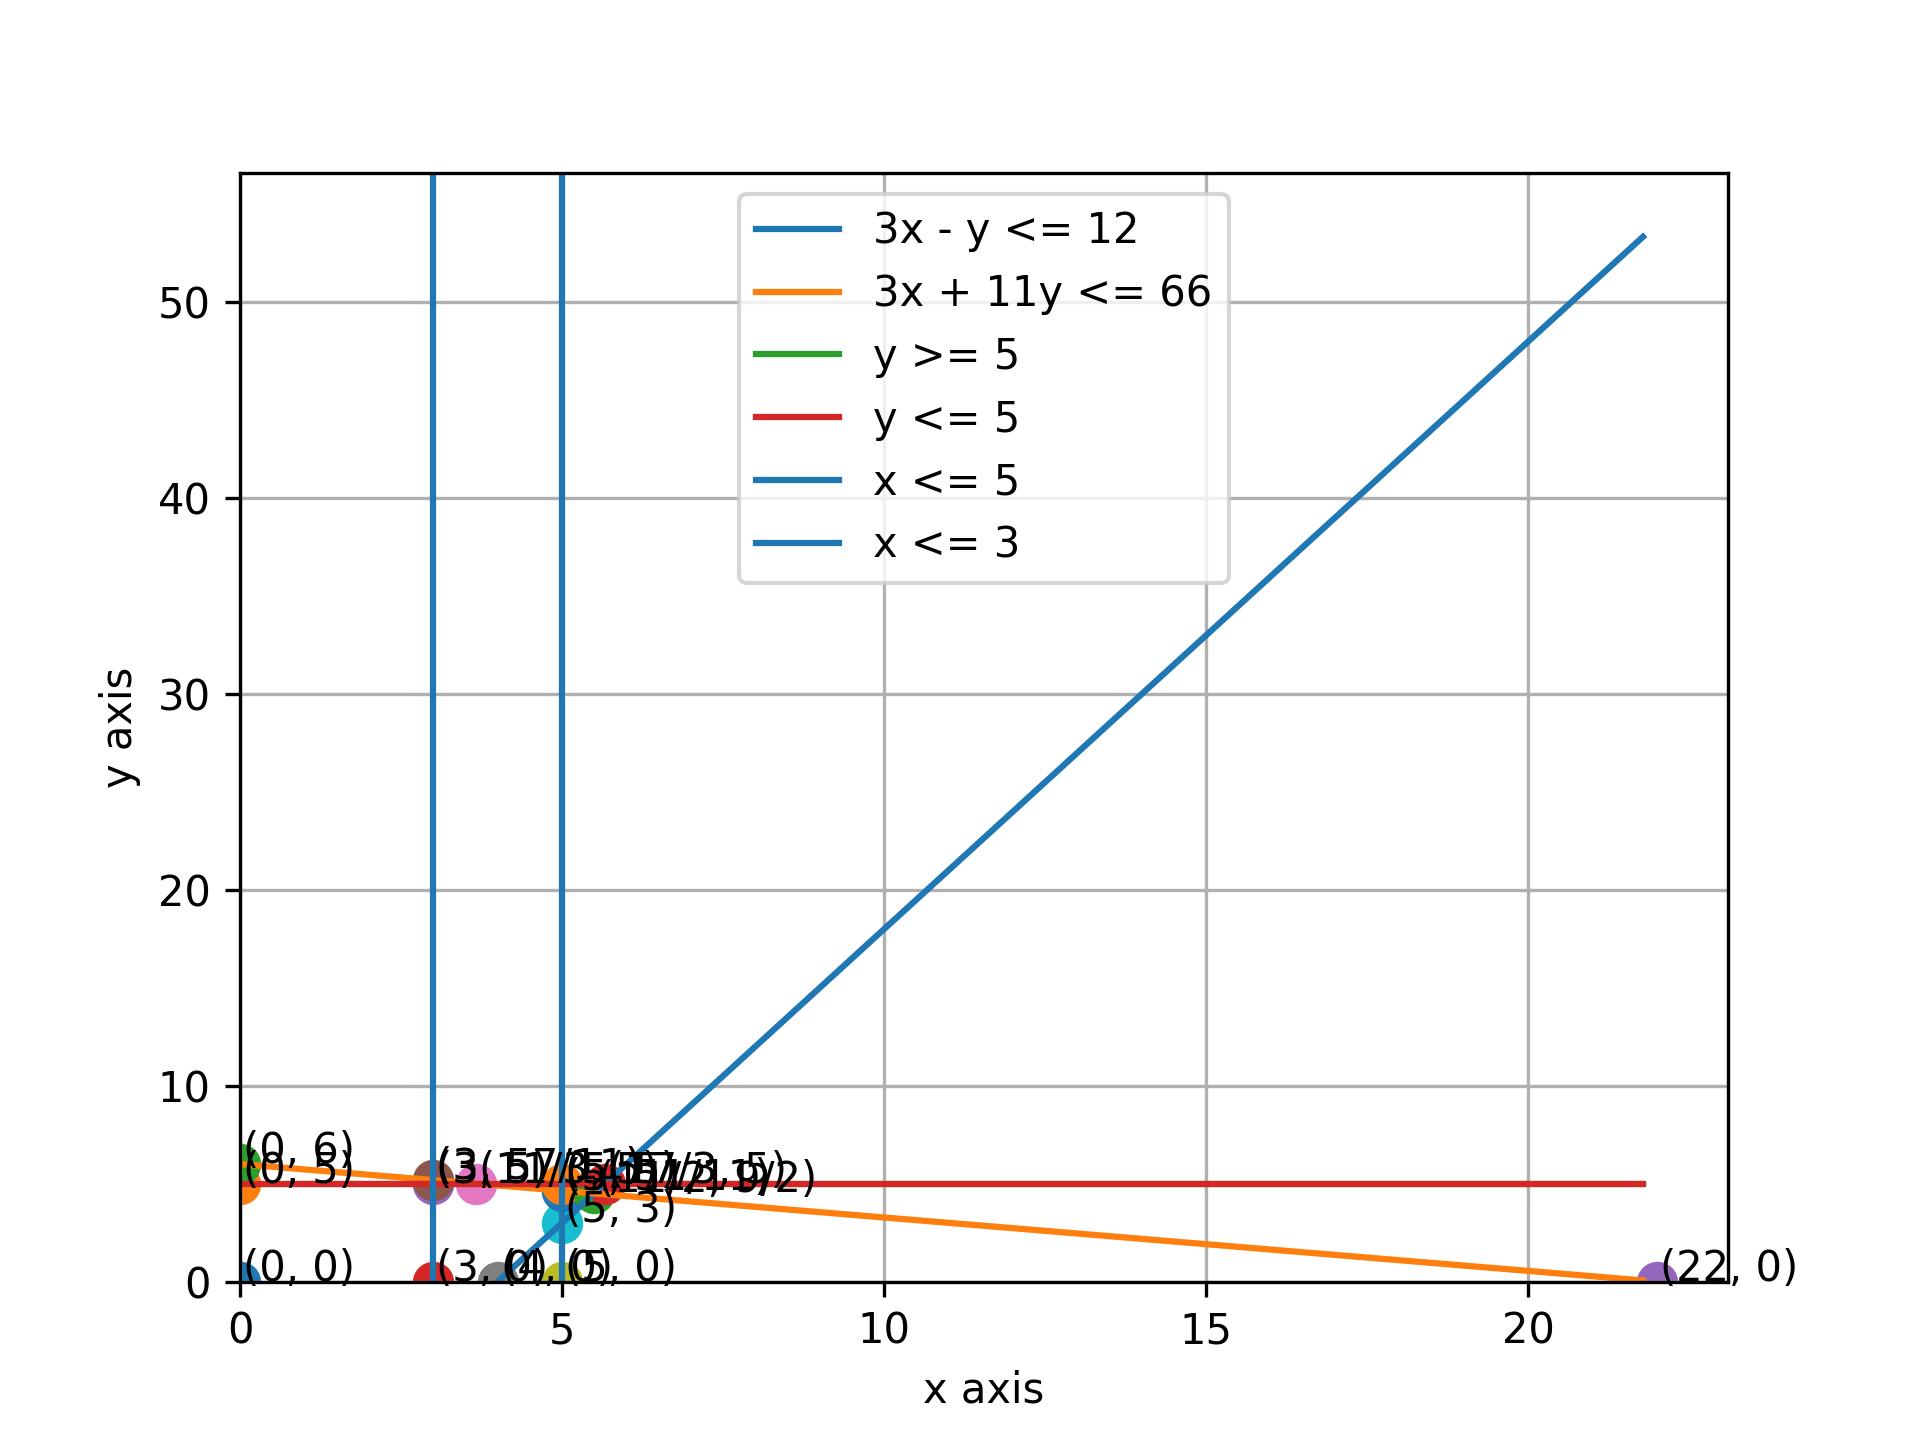
\includegraphics[width=0.6\textwidth]{outputs/ipp4/graph8.png}
\end{center}
\begin{align*}
Z=29\end{align*}
\begin{align*}
x=3\end{align*}
\begin{align*}
y=5\end{align*}
\begin{align*}
\text{Maximize} \quad & 3x + 4y\\
\text{subject to} \quad
& 3x - y\le12\\
& 3x + 11y\le66\\
& x\le5\\
& y\ge5\\
& x\le3\\
& y\ge6\\
& x\ge0,\; y\ge0\end{align*}
\begin{align*}
3x - y=12\end{align*}
\begin{align*}
3x + 11y=66\end{align*}
Gauss Elimination:\\
Echelon Form:\\
\begin{align*}
\left(
\begin{array}{cc|c}
3 & -1 & 12\\
3 & 11 & 66\\
\end{array}
\right)_{2\times 3}
\end{align*}
\begin{align*}
\left(
\begin{array}{cc|c}
3 & -1 & 12\\
0 & 12 & 54\\
\end{array}
\right)_{2\times 3}
\end{align*}
\begin{align*}
\left(
\begin{array}{cc|c}
3 & -1 & 12\\
0 & 12 & 54\\
\end{array}
\right)_{2\times 3}
\end{align*}
\begin{align*}
x=\frac{11}{2}\end{align*}
\begin{align*}
y=\frac{9}{2}\end{align*}
\begin{align*}
3x - y=12\end{align*}
\begin{align*}
x=5\end{align*}
Gauss Elimination:\\
Echelon Form:\\
\begin{align*}
\left(
\begin{array}{cc|c}
3 & -1 & 12\\
1 & 0 & 5\\
\end{array}
\right)_{2\times 3}
\end{align*}
\begin{align*}
\left(
\begin{array}{cc|c}
3 & -1 & 12\\
0 & \frac{1}{3} & 1\\
\end{array}
\right)_{2\times 3}
\end{align*}
\begin{align*}
\left(
\begin{array}{cc|c}
3 & -1 & 12\\
0 & \frac{1}{3} & 1\\
\end{array}
\right)_{2\times 3}
\end{align*}
\begin{align*}
x=5\end{align*}
\begin{align*}
y=3\end{align*}
\begin{align*}
3x - y=12\end{align*}
\begin{align*}
y=5\end{align*}
Gauss Elimination:\\
Echelon Form:\\
\begin{align*}
\left(
\begin{array}{cc|c}
3 & -1 & 12\\
0 & 1 & 5\\
\end{array}
\right)_{2\times 3}
\end{align*}
\begin{align*}
\left(
\begin{array}{cc|c}
3 & -1 & 12\\
0 & 1 & 5\\
\end{array}
\right)_{2\times 3}
\end{align*}
\begin{align*}
\left(
\begin{array}{cc|c}
3 & -1 & 12\\
0 & 1 & 5\\
\end{array}
\right)_{2\times 3}
\end{align*}
\begin{align*}
x=\frac{17}{3}\end{align*}
\begin{align*}
y=5\end{align*}
\begin{align*}
3x - y=12\end{align*}
\begin{align*}
x=3\end{align*}
Gauss Elimination:\\
Echelon Form:\\
\begin{align*}
\left(
\begin{array}{cc|c}
3 & -1 & 12\\
1 & 0 & 3\\
\end{array}
\right)_{2\times 3}
\end{align*}
\begin{align*}
\left(
\begin{array}{cc|c}
3 & -1 & 12\\
0 & \frac{1}{3} & -1\\
\end{array}
\right)_{2\times 3}
\end{align*}
\begin{align*}
\left(
\begin{array}{cc|c}
3 & -1 & 12\\
0 & \frac{1}{3} & -1\\
\end{array}
\right)_{2\times 3}
\end{align*}
\begin{align*}
x=3\end{align*}
\begin{align*}
y=-3\end{align*}
\begin{align*}
3x - y=12\end{align*}
\begin{align*}
y=6\end{align*}
Gauss Elimination:\\
Echelon Form:\\
\begin{align*}
\left(
\begin{array}{cc|c}
3 & -1 & 12\\
0 & 1 & 6\\
\end{array}
\right)_{2\times 3}
\end{align*}
\begin{align*}
\left(
\begin{array}{cc|c}
3 & -1 & 12\\
0 & 1 & 6\\
\end{array}
\right)_{2\times 3}
\end{align*}
\begin{align*}
\left(
\begin{array}{cc|c}
3 & -1 & 12\\
0 & 1 & 6\\
\end{array}
\right)_{2\times 3}
\end{align*}
\begin{align*}
x=6\end{align*}
\begin{align*}
y=6\end{align*}
\begin{align*}
3x + 11y=66\end{align*}
\begin{align*}
x=5\end{align*}
Gauss Elimination:\\
Echelon Form:\\
\begin{align*}
\left(
\begin{array}{cc|c}
3 & 11 & 66\\
1 & 0 & 5\\
\end{array}
\right)_{2\times 3}
\end{align*}
\begin{align*}
\left(
\begin{array}{cc|c}
3 & 11 & 66\\
0 & -\frac{11}{3} & -17\\
\end{array}
\right)_{2\times 3}
\end{align*}
\begin{align*}
\left(
\begin{array}{cc|c}
3 & 11 & 66\\
0 & -\frac{11}{3} & -17\\
\end{array}
\right)_{2\times 3}
\end{align*}
\begin{align*}
x=5\end{align*}
\begin{align*}
y=\frac{51}{11}\end{align*}
\begin{align*}
3x + 11y=66\end{align*}
\begin{align*}
y=5\end{align*}
Gauss Elimination:\\
Echelon Form:\\
\begin{align*}
\left(
\begin{array}{cc|c}
3 & 11 & 66\\
0 & 1 & 5\\
\end{array}
\right)_{2\times 3}
\end{align*}
\begin{align*}
\left(
\begin{array}{cc|c}
3 & 11 & 66\\
0 & 1 & 5\\
\end{array}
\right)_{2\times 3}
\end{align*}
\begin{align*}
\left(
\begin{array}{cc|c}
3 & 11 & 66\\
0 & 1 & 5\\
\end{array}
\right)_{2\times 3}
\end{align*}
\begin{align*}
x=\frac{11}{3}\end{align*}
\begin{align*}
y=5\end{align*}
\begin{align*}
3x + 11y=66\end{align*}
\begin{align*}
x=3\end{align*}
Gauss Elimination:\\
Echelon Form:\\
\begin{align*}
\left(
\begin{array}{cc|c}
3 & 11 & 66\\
1 & 0 & 3\\
\end{array}
\right)_{2\times 3}
\end{align*}
\begin{align*}
\left(
\begin{array}{cc|c}
3 & 11 & 66\\
0 & -\frac{11}{3} & -19\\
\end{array}
\right)_{2\times 3}
\end{align*}
\begin{align*}
\left(
\begin{array}{cc|c}
3 & 11 & 66\\
0 & -\frac{11}{3} & -19\\
\end{array}
\right)_{2\times 3}
\end{align*}
\begin{align*}
x=3\end{align*}
\begin{align*}
y=\frac{57}{11}\end{align*}
\begin{align*}
3x + 11y=66\end{align*}
\begin{align*}
y=6\end{align*}
Gauss Elimination:\\
Echelon Form:\\
\begin{align*}
\left(
\begin{array}{cc|c}
3 & 11 & 66\\
0 & 1 & 6\\
\end{array}
\right)_{2\times 3}
\end{align*}
\begin{align*}
\left(
\begin{array}{cc|c}
3 & 11 & 66\\
0 & 1 & 6\\
\end{array}
\right)_{2\times 3}
\end{align*}
\begin{align*}
\left(
\begin{array}{cc|c}
3 & 11 & 66\\
0 & 1 & 6\\
\end{array}
\right)_{2\times 3}
\end{align*}
\begin{align*}
x=0\end{align*}
\begin{align*}
y=6\end{align*}
\begin{align*}
x=5\end{align*}
\begin{align*}
y=5\end{align*}
Gauss Elimination:\\
Echelon Form:\\
\begin{align*}
\left(
\begin{array}{cc|c}
1 & 0 & 5\\
0 & 1 & 5\\
\end{array}
\right)_{2\times 3}
\end{align*}
\begin{align*}
\left(
\begin{array}{cc|c}
1 & 0 & 5\\
0 & 1 & 5\\
\end{array}
\right)_{2\times 3}
\end{align*}
\begin{align*}
\left(
\begin{array}{cc|c}
1 & 0 & 5\\
0 & 1 & 5\\
\end{array}
\right)_{2\times 3}
\end{align*}
\begin{align*}
x=5\end{align*}
\begin{align*}
y=5\end{align*}
\begin{align*}
x=5\end{align*}
\begin{align*}
x=3\end{align*}
Gauss Elimination:\\
Echelon Form:\\
\begin{align*}
\left(
\begin{array}{c|c}
1 & 5\\
1 & 3\\
\end{array}
\right)_{2\times 2}
\end{align*}
\begin{align*}
\left(
\begin{array}{c|c}
1 & 5\\
0 & -2\\
\end{array}
\right)_{2\times 2}
\end{align*}
\begin{align*}
\left(
\begin{array}{c|c}
1 & 5\\
0 & -2\\
\end{array}
\right)_{2\times 2}
\end{align*}
No solution\\
\begin{align*}
x=5\end{align*}
\begin{align*}
y=6\end{align*}
Gauss Elimination:\\
Echelon Form:\\
\begin{align*}
\left(
\begin{array}{cc|c}
1 & 0 & 5\\
0 & 1 & 6\\
\end{array}
\right)_{2\times 3}
\end{align*}
\begin{align*}
\left(
\begin{array}{cc|c}
1 & 0 & 5\\
0 & 1 & 6\\
\end{array}
\right)_{2\times 3}
\end{align*}
\begin{align*}
\left(
\begin{array}{cc|c}
1 & 0 & 5\\
0 & 1 & 6\\
\end{array}
\right)_{2\times 3}
\end{align*}
\begin{align*}
x=5\end{align*}
\begin{align*}
y=6\end{align*}
\begin{align*}
y=5\end{align*}
\begin{align*}
x=3\end{align*}
Gauss Elimination:\\
Echelon Form:\\
\begin{align*}
\left(
\begin{array}{cc|c}
0 & 1 & 5\\
1 & 0 & 3\\
\end{array}
\right)_{2\times 3}
\end{align*}
\begin{align*}
\left(
\begin{array}{cc|c}
1 & 0 & 3\\
0 & 1 & 5\\
\end{array}
\right)_{2\times 3}
\end{align*}
\begin{align*}
\left(
\begin{array}{cc|c}
1 & 0 & 3\\
0 & 1 & 5\\
\end{array}
\right)_{2\times 3}
\end{align*}
\begin{align*}
x=3\end{align*}
\begin{align*}
y=5\end{align*}
\begin{align*}
y=5\end{align*}
\begin{align*}
y=6\end{align*}
Gauss Elimination:\\
Echelon Form:\\
\begin{align*}
\left(
\begin{array}{c|c}
1 & 5\\
1 & 6\\
\end{array}
\right)_{2\times 2}
\end{align*}
\begin{align*}
\left(
\begin{array}{c|c}
1 & 5\\
0 & 1\\
\end{array}
\right)_{2\times 2}
\end{align*}
\begin{align*}
\left(
\begin{array}{c|c}
1 & 5\\
0 & 1\\
\end{array}
\right)_{2\times 2}
\end{align*}
No solution\\
\begin{align*}
x=3\end{align*}
\begin{align*}
y=6\end{align*}
Gauss Elimination:\\
Echelon Form:\\
\begin{align*}
\left(
\begin{array}{cc|c}
1 & 0 & 3\\
0 & 1 & 6\\
\end{array}
\right)_{2\times 3}
\end{align*}
\begin{align*}
\left(
\begin{array}{cc|c}
1 & 0 & 3\\
0 & 1 & 6\\
\end{array}
\right)_{2\times 3}
\end{align*}
\begin{align*}
\left(
\begin{array}{cc|c}
1 & 0 & 3\\
0 & 1 & 6\\
\end{array}
\right)_{2\times 3}
\end{align*}
\begin{align*}
x=3\end{align*}
\begin{align*}
y=6\end{align*}
\begin{center}
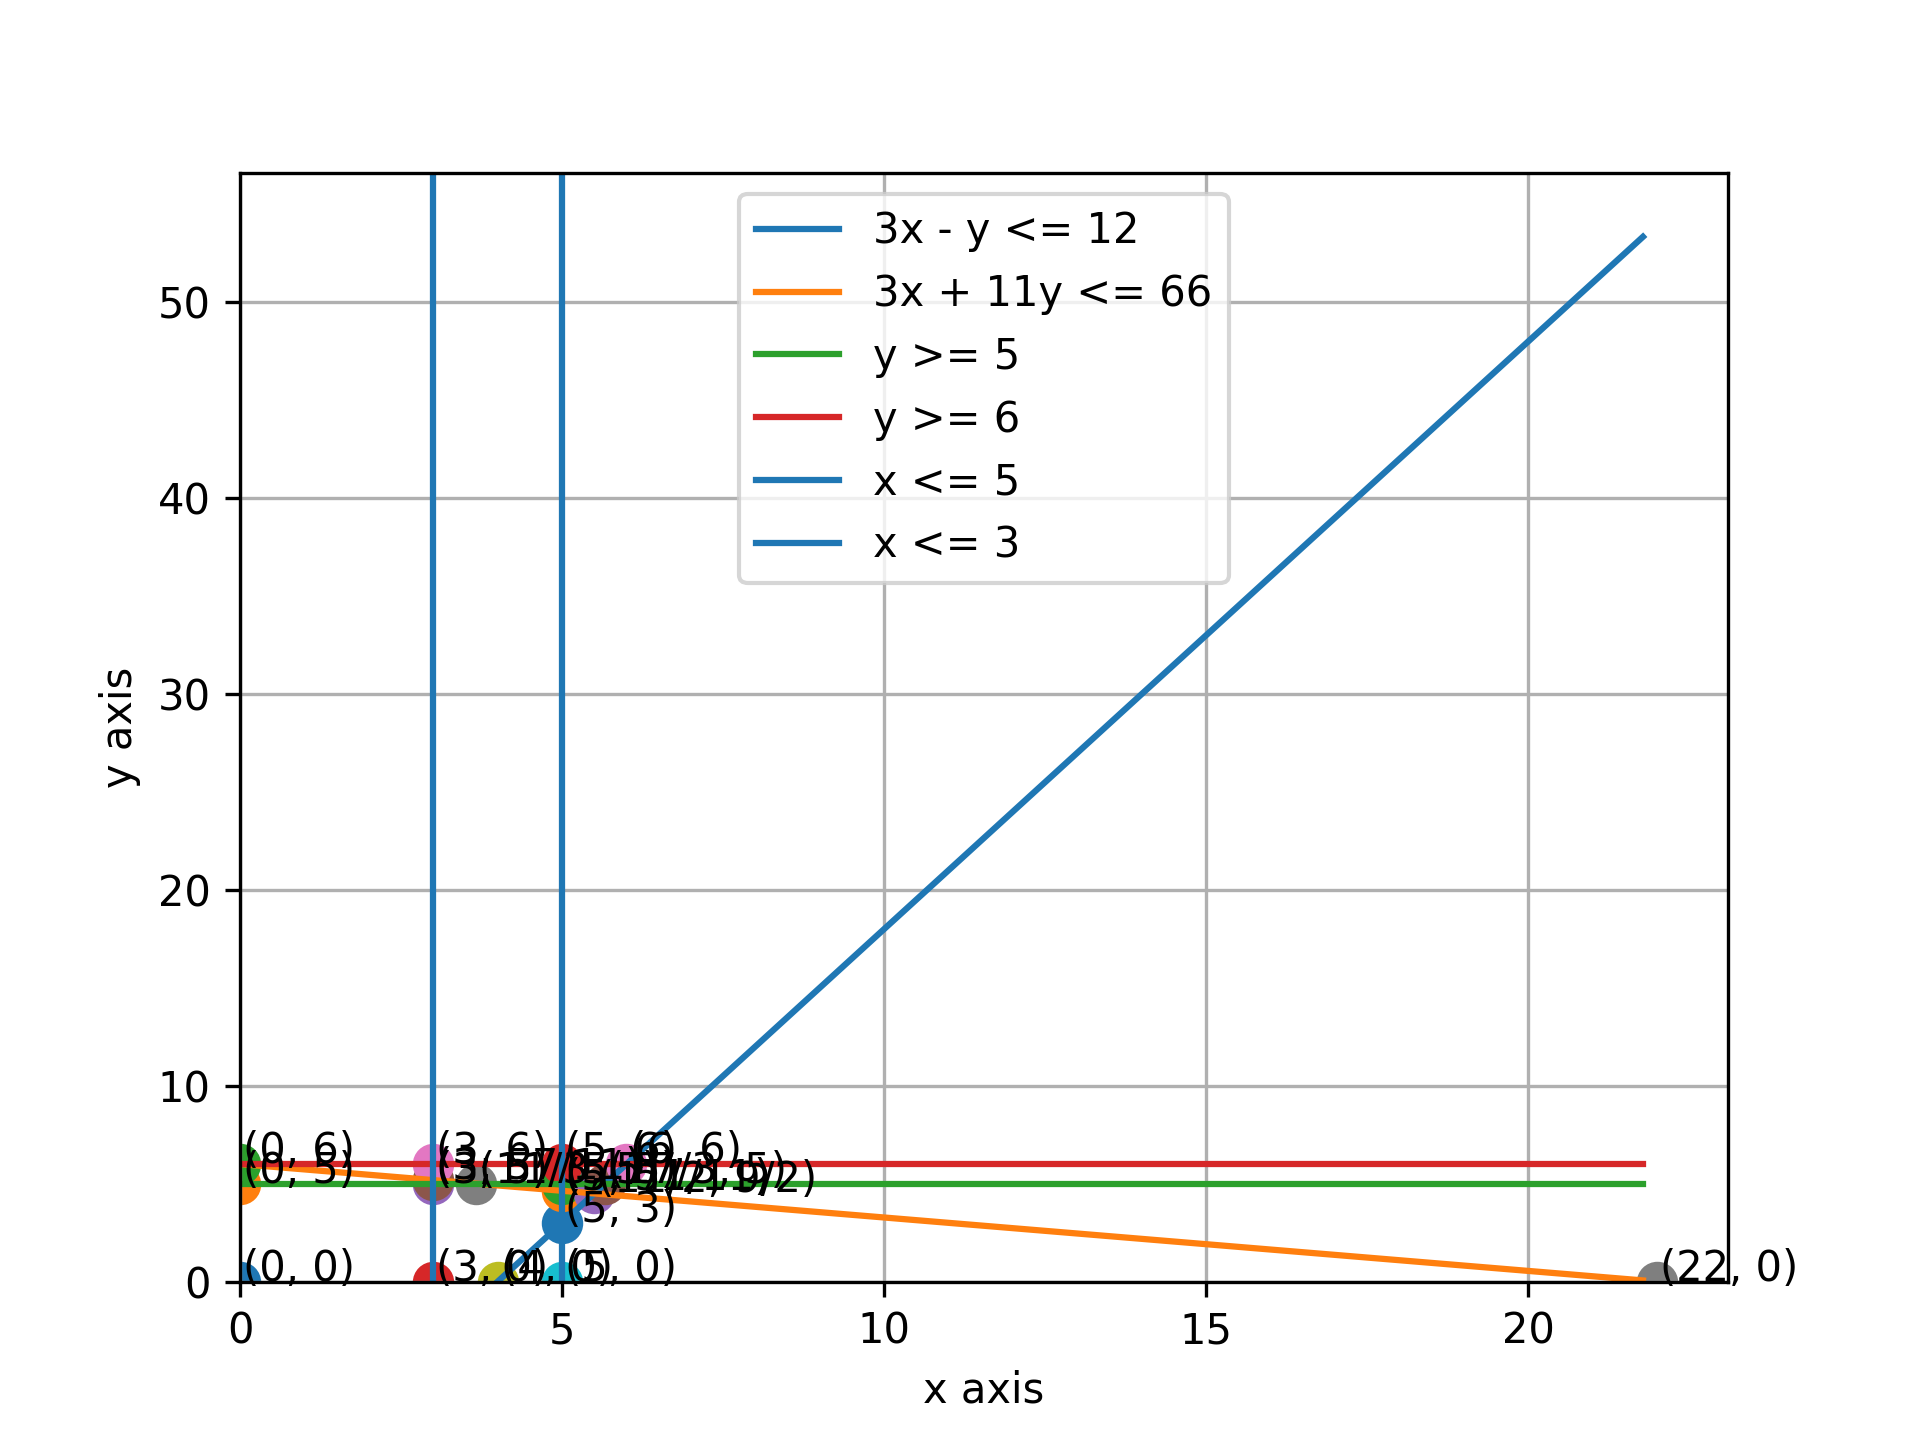
\includegraphics[width=0.6\textwidth]{outputs/ipp4/graph9.png}
\end{center}
\begin{align*}
Z=24\end{align*}
\begin{align*}
x=0\end{align*}
\begin{align*}
y=6\end{align*}
\begin{align*}
Z=31\end{align*}
\begin{align*}
x=5\end{align*}
\begin{align*}
y=4\end{align*}
\begin{align*}
\text{Minimize} \quad & 2x + 3y\\
\text{subject to} \quad
& 2x + 3y\le7\\
& x\le2\\
& y\le2\\
& x\ge0,\; y\ge0\end{align*}
\begin{align*}
2x + 3y=7\end{align*}
\begin{align*}
x=2\end{align*}
Gauss Elimination:\\
Echelon Form:\\
\begin{align*}
\left(
\begin{array}{cc|c}
2 & 3 & 7\\
1 & 0 & 2\\
\end{array}
\right)_{2\times 3}
\end{align*}
\begin{align*}
\left(
\begin{array}{cc|c}
2 & 3 & 7\\
0 & -\frac{3}{2} & -\frac{3}{2}\\
\end{array}
\right)_{2\times 3}
\end{align*}
\begin{align*}
\left(
\begin{array}{cc|c}
2 & 3 & 7\\
0 & -\frac{3}{2} & -\frac{3}{2}\\
\end{array}
\right)_{2\times 3}
\end{align*}
\begin{align*}
x=2\end{align*}
\begin{align*}
y=1\end{align*}
\begin{align*}
2x + 3y=7\end{align*}
\begin{align*}
y=2\end{align*}
Gauss Elimination:\\
Echelon Form:\\
\begin{align*}
\left(
\begin{array}{cc|c}
2 & 3 & 7\\
0 & 1 & 2\\
\end{array}
\right)_{2\times 3}
\end{align*}
\begin{align*}
\left(
\begin{array}{cc|c}
2 & 3 & 7\\
0 & 1 & 2\\
\end{array}
\right)_{2\times 3}
\end{align*}
\begin{align*}
\left(
\begin{array}{cc|c}
2 & 3 & 7\\
0 & 1 & 2\\
\end{array}
\right)_{2\times 3}
\end{align*}
\begin{align*}
x=\frac{1}{2}\end{align*}
\begin{align*}
y=2\end{align*}
\begin{align*}
x=2\end{align*}
\begin{align*}
y=2\end{align*}
Gauss Elimination:\\
Echelon Form:\\
\begin{align*}
\left(
\begin{array}{cc|c}
1 & 0 & 2\\
0 & 1 & 2\\
\end{array}
\right)_{2\times 3}
\end{align*}
\begin{align*}
\left(
\begin{array}{cc|c}
1 & 0 & 2\\
0 & 1 & 2\\
\end{array}
\right)_{2\times 3}
\end{align*}
\begin{align*}
\left(
\begin{array}{cc|c}
1 & 0 & 2\\
0 & 1 & 2\\
\end{array}
\right)_{2\times 3}
\end{align*}
\begin{align*}
x=2\end{align*}
\begin{align*}
y=2\end{align*}
\begin{center}
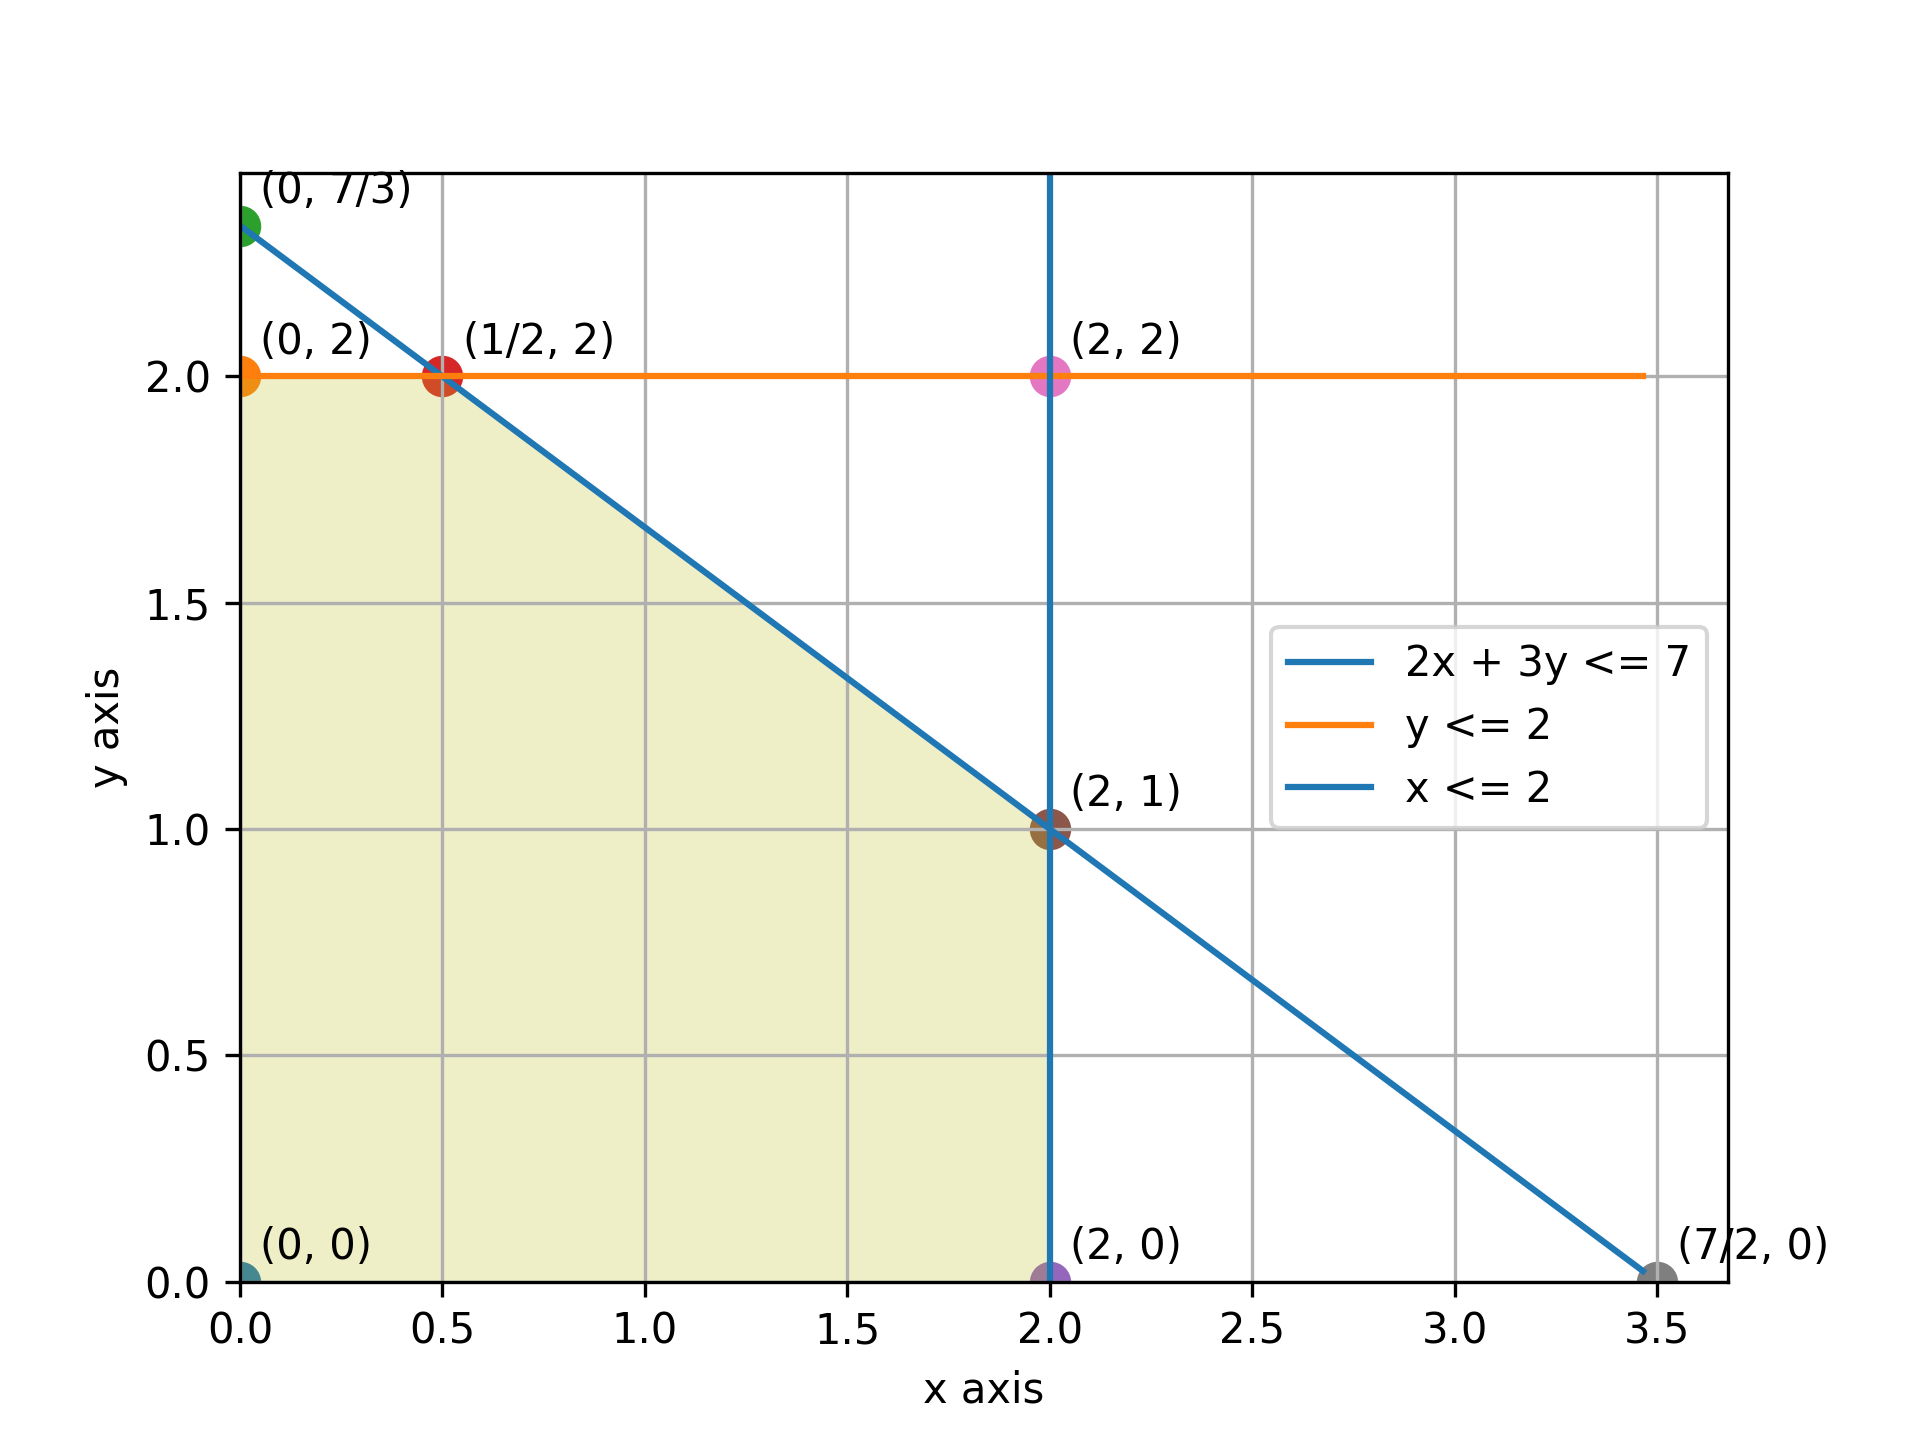
\includegraphics[width=0.6\textwidth]{outputs/ipp5/graph1.png}
\end{center}
\begin{align*}
Z=0\end{align*}
\begin{align*}
x=0\end{align*}
\begin{align*}
y=0\end{align*}
\begin{align*}
Z=0\end{align*}
\begin{align*}
x=0\end{align*}
\begin{align*}
y=0\end{align*}
\begin{align*}
\text{Maximize} \quad & 6x_{1}^{2} + 5x_{2}^{2}\\
\text{subject to} \quad
& x_{1} + 5x_{2}=3\\
& x_{1}\ge0,\; x_{2}\ge0\end{align*}
\begin{align*}
\lambda=6x_{1}^{2} + 5x_{2}^{2} + 3\lambda_{1} - \lambda_{1}x_{1} - 5\lambda_{1}x_{2}\end{align*}
\begin{align*}
\dfrac{d}{dx_{1}}6x_{1}^{2} + 5x_{2}^{2} + 3\lambda_{1} - \lambda_{1}x_{1} - 5\lambda_{1}x_{2}=-\lambda_{1} + 12x_{1}\end{align*}
\begin{align*}
\dfrac{d}{dx_{2}}6x_{1}^{2} + 5x_{2}^{2} + 3\lambda_{1} - \lambda_{1}x_{1} - 5\lambda_{1}x_{2}=-5\lambda_{1} + 10x_{2}\end{align*}
\begin{align*}
\dfrac{d}{d\lambda_{1}}6x_{1}^{2} + 5x_{2}^{2} + 3\lambda_{1} - \lambda_{1}x_{1} - 5\lambda_{1}x_{2}=-x_{1} - 5x_{2} + 3\end{align*}
\begin{align*}
-\lambda_{1} + 12x_{1}=0\end{align*}
\begin{align*}
-5\lambda_{1} + 10x_{2}=0\end{align*}
\begin{align*}
-x_{1} - 5x_{2}=-3\end{align*}
Gauss Elimination:\\
Echelon Form:\\
\begin{align*}
\left(
\begin{array}{ccc|c}
-1 & 12 & 0 & 0\\
-5 & 0 & 10 & 0\\
0 & -1 & -5 & -3\\
\end{array}
\right)_{3\times 4}
\end{align*}
\begin{align*}
\left(
\begin{array}{ccc|c}
-1 & 12 & 0 & 0\\
0 & -60 & 10 & 0\\
0 & -1 & -5 & -3\\
\end{array}
\right)_{3\times 4}
\end{align*}
\begin{align*}
\left(
\begin{array}{ccc|c}
-1 & 12 & 0 & 0\\
0 & -60 & 10 & 0\\
0 & 0 & -\frac{31}{6} & -3\\
\end{array}
\right)_{3\times 4}
\end{align*}
\begin{align*}
\left(
\begin{array}{ccc|c}
-1 & 12 & 0 & 0\\
0 & -60 & 10 & 0\\
0 & 0 & -\frac{31}{6} & -3\\
\end{array}
\right)_{3\times 4}
\end{align*}
\begin{align*}
\lambda_{1}=\frac{36}{31}\end{align*}
\begin{align*}
x_{1}=\frac{3}{31}\end{align*}
\begin{align*}
x_{2}=\frac{18}{31}\end{align*}
\begin{align*}
\left.6x_{1}^{2} + 5x_{2}^{2}\right|_{x_{1}=\frac{3}{31},x_{2}=\frac{18}{31}}=\frac{54}{31}\end{align*}
\begin{align*}
Z=\frac{54}{31}\end{align*}
\begin{align*}
x_{1}=\frac{3}{31}\end{align*}
\begin{align*}
x_{2}=\frac{18}{31}\end{align*}
\begin{align*}
\text{Maximize} \quad & 2x_{1}^{2} + 2x_{2}^{2} + 2x_{3}^{2} - 24x_{1} - 8x_{2} - 12x_{3} + 200\\
\text{subject to} \quad
& x_{1} + x_{2} + x_{3}=11\\
& x_{1}\ge0,\; x_{2}\ge0,\; x_{3}\ge0\end{align*}
\begin{align*}
\lambda=2x_{1}^{2} + 2x_{2}^{2} + 2x_{3}^{2} + 11\lambda_{1} - \lambda_{1}x_{1} - \lambda_{1}x_{2} - \lambda_{1}x_{3} - 24x_{1} - 8x_{2} - 12x_{3} + 200\end{align*}
\begin{align*}
\dfrac{d}{dx_{1}}2x_{1}^{2} + 2x_{2}^{2} + 2x_{3}^{2} + 11\lambda_{1} - \lambda_{1}x_{1} - \lambda_{1}x_{2} - \lambda_{1}x_{3} - 24x_{1} - 8x_{2} - 12x_{3} + 200=-\lambda_{1} + 4x_{1} - 24\end{align*}
\begin{align*}
\dfrac{d}{dx_{2}}2x_{1}^{2} + 2x_{2}^{2} + 2x_{3}^{2} + 11\lambda_{1} - \lambda_{1}x_{1} - \lambda_{1}x_{2} - \lambda_{1}x_{3} - 24x_{1} - 8x_{2} - 12x_{3} + 200=-\lambda_{1} + 4x_{2} - 8\end{align*}
\begin{align*}
\dfrac{d}{dx_{3}}2x_{1}^{2} + 2x_{2}^{2} + 2x_{3}^{2} + 11\lambda_{1} - \lambda_{1}x_{1} - \lambda_{1}x_{2} - \lambda_{1}x_{3} - 24x_{1} - 8x_{2} - 12x_{3} + 200=-\lambda_{1} + 4x_{3} - 12\end{align*}
\begin{align*}
\dfrac{d}{d\lambda_{1}}2x_{1}^{2} + 2x_{2}^{2} + 2x_{3}^{2} + 11\lambda_{1} - \lambda_{1}x_{1} - \lambda_{1}x_{2} - \lambda_{1}x_{3} - 24x_{1} - 8x_{2} - 12x_{3} + 200=-x_{1} - x_{2} - x_{3} + 11\end{align*}
\begin{align*}
-\lambda_{1} + 4x_{1}=24\end{align*}
\begin{align*}
-\lambda_{1} + 4x_{2}=8\end{align*}
\begin{align*}
-\lambda_{1} + 4x_{3}=12\end{align*}
\begin{align*}
-x_{1} - x_{2} - x_{3}=-11\end{align*}
Gauss Elimination:\\
Echelon Form:\\
\begin{align*}
\left(
\begin{array}{cccc|c}
-1 & 4 & 0 & 0 & 24\\
-1 & 0 & 4 & 0 & 8\\
-1 & 0 & 0 & 4 & 12\\
0 & -1 & -1 & -1 & -11\\
\end{array}
\right)_{4\times 5}
\end{align*}
\begin{align*}
\left(
\begin{array}{cccc|c}
-1 & 4 & 0 & 0 & 24\\
0 & -4 & 4 & 0 & -16\\
0 & -4 & 0 & 4 & -12\\
0 & -1 & -1 & -1 & -11\\
\end{array}
\right)_{4\times 5}
\end{align*}
\begin{align*}
\left(
\begin{array}{cccc|c}
-1 & 4 & 0 & 0 & 24\\
0 & -4 & 4 & 0 & -16\\
0 & 0 & -4 & 4 & 4\\
0 & 0 & -2 & -1 & -7\\
\end{array}
\right)_{4\times 5}
\end{align*}
\begin{align*}
\left(
\begin{array}{cccc|c}
-1 & 4 & 0 & 0 & 24\\
0 & -4 & 4 & 0 & -16\\
0 & 0 & -4 & 4 & 4\\
0 & 0 & 0 & -3 & -9\\
\end{array}
\right)_{4\times 5}
\end{align*}
\begin{align*}
\left(
\begin{array}{cccc|c}
-1 & 4 & 0 & 0 & 24\\
0 & -4 & 4 & 0 & -16\\
0 & 0 & -4 & 4 & 4\\
0 & 0 & 0 & -3 & -9\\
\end{array}
\right)_{4\times 5}
\end{align*}
\begin{align*}
\lambda_{1}=0\end{align*}
\begin{align*}
x_{1}=6\end{align*}
\begin{align*}
x_{2}=2\end{align*}
\begin{align*}
x_{3}=3\end{align*}
Sufficiency Test:\\
Determinant:\\
Echelon Form:\\
\begin{align*}
\begin{vmatrix}
0 & 1 & 1\\
1 & 4 & 0\\
1 & 0 & 4\\
\end{vmatrix}_{3\times 3}
\end{align*}
\begin{align*}
\begin{vmatrix}
1 & 4 & 0\\
0 & 1 & 1\\
0 & -4 & 4\\
\end{vmatrix}_{3\times 3}
\end{align*}
\begin{align*}
\begin{vmatrix}
1 & 4 & 0\\
0 & 1 & 1\\
0 & 0 & 8\\
\end{vmatrix}_{3\times 3}
\end{align*}
\begin{align*}
\begin{vmatrix}
1 & 4 & 0\\
0 & 1 & 1\\
0 & 0 & 8\\
\end{vmatrix}_{3\times 3}
\end{align*}
\begin{align*}
\left.2x_{1}^{2} + 2x_{2}^{2} + 2x_{3}^{2} - 24x_{1} - 8x_{2} - 12x_{3} + 200\right|_{x_{1}=6,x_{2}=2,x_{3}=3}=102\end{align*}
\begin{align*}
Z=102\end{align*}
\begin{align*}
x_{1}=6\end{align*}
\begin{align*}
x_{2}=2\end{align*}
\begin{align*}
x_{3}=3\end{align*}
\begin{align*}
\text{Minimize} \quad & x_{1}^{2} + x_{2}^{2} + x_{3}^{2}\\
\text{subject to} \quad
& x_{1} + x_{2} + 3x_{3}=2\\
& 5x_{1} + 2x_{2} + x_{3}=5\\
& x_{1}\ge0,\; x_{2}\ge0,\; x_{3}\ge0\end{align*}
\begin{align*}
\lambda=x_{1}^{2} + x_{2}^{2} + x_{3}^{2} + 2\lambda_{1} - \lambda_{1}x_{1} - \lambda_{1}x_{2} - 3\lambda_{1}x_{3} + 5\lambda_{2} - 5\lambda_{2}x_{1} - 2\lambda_{2}x_{2} - \lambda_{2}x_{3}\end{align*}
\begin{align*}
\dfrac{d}{dx_{1}}x_{1}^{2} + x_{2}^{2} + x_{3}^{2} + 2\lambda_{1} - \lambda_{1}x_{1} - \lambda_{1}x_{2} - 3\lambda_{1}x_{3} + 5\lambda_{2} - 5\lambda_{2}x_{1} - 2\lambda_{2}x_{2} - \lambda_{2}x_{3}=-\lambda_{1} - 5\lambda_{2} + 2x_{1}\end{align*}
\begin{align*}
\dfrac{d}{dx_{2}}x_{1}^{2} + x_{2}^{2} + x_{3}^{2} + 2\lambda_{1} - \lambda_{1}x_{1} - \lambda_{1}x_{2} - 3\lambda_{1}x_{3} + 5\lambda_{2} - 5\lambda_{2}x_{1} - 2\lambda_{2}x_{2} - \lambda_{2}x_{3}=-\lambda_{1} - 2\lambda_{2} + 2x_{2}\end{align*}
\begin{align*}
\dfrac{d}{dx_{3}}x_{1}^{2} + x_{2}^{2} + x_{3}^{2} + 2\lambda_{1} - \lambda_{1}x_{1} - \lambda_{1}x_{2} - 3\lambda_{1}x_{3} + 5\lambda_{2} - 5\lambda_{2}x_{1} - 2\lambda_{2}x_{2} - \lambda_{2}x_{3}=-3\lambda_{1} - \lambda_{2} + 2x_{3}\end{align*}
\begin{align*}
\dfrac{d}{d\lambda_{1}}x_{1}^{2} + x_{2}^{2} + x_{3}^{2} + 2\lambda_{1} - \lambda_{1}x_{1} - \lambda_{1}x_{2} - 3\lambda_{1}x_{3} + 5\lambda_{2} - 5\lambda_{2}x_{1} - 2\lambda_{2}x_{2} - \lambda_{2}x_{3}=-x_{1} - x_{2} - 3x_{3} + 2\end{align*}
\begin{align*}
\dfrac{d}{d\lambda_{2}}x_{1}^{2} + x_{2}^{2} + x_{3}^{2} + 2\lambda_{1} - \lambda_{1}x_{1} - \lambda_{1}x_{2} - 3\lambda_{1}x_{3} + 5\lambda_{2} - 5\lambda_{2}x_{1} - 2\lambda_{2}x_{2} - \lambda_{2}x_{3}=-5x_{1} - 2x_{2} - x_{3} + 5\end{align*}
\begin{align*}
-\lambda_{1} - 5\lambda_{2} + 2x_{1}=0\end{align*}
\begin{align*}
-\lambda_{1} - 2\lambda_{2} + 2x_{2}=0\end{align*}
\begin{align*}
-3\lambda_{1} - \lambda_{2} + 2x_{3}=0\end{align*}
\begin{align*}
-x_{1} - x_{2} - 3x_{3}=-2\end{align*}
\begin{align*}
-5x_{1} - 2x_{2} - x_{3}=-5\end{align*}
Gauss Elimination:\\
Echelon Form:\\
\begin{align*}
\left(
\begin{array}{ccccc|c}
-1 & -5 & 2 & 0 & 0 & 0\\
-1 & -2 & 0 & 2 & 0 & 0\\
-3 & -1 & 0 & 0 & 2 & 0\\
0 & 0 & -1 & -1 & -3 & -2\\
0 & 0 & -5 & -2 & -1 & -5\\
\end{array}
\right)_{5\times 6}
\end{align*}
\begin{align*}
\left(
\begin{array}{ccccc|c}
-1 & -5 & 2 & 0 & 0 & 0\\
0 & 3 & -2 & 2 & 0 & 0\\
0 & 14 & -6 & 0 & 2 & 0\\
0 & 0 & -1 & -1 & -3 & -2\\
0 & 0 & -5 & -2 & -1 & -5\\
\end{array}
\right)_{5\times 6}
\end{align*}
\begin{align*}
\left(
\begin{array}{ccccc|c}
-1 & -5 & 2 & 0 & 0 & 0\\
0 & 3 & -2 & 2 & 0 & 0\\
0 & 0 & \frac{10}{3} & -\frac{28}{3} & 2 & 0\\
0 & 0 & -1 & -1 & -3 & -2\\
0 & 0 & -5 & -2 & -1 & -5\\
\end{array}
\right)_{5\times 6}
\end{align*}
\begin{align*}
\left(
\begin{array}{ccccc|c}
-1 & -5 & 2 & 0 & 0 & 0\\
0 & 3 & -2 & 2 & 0 & 0\\
0 & 0 & \frac{10}{3} & -\frac{28}{3} & 2 & 0\\
0 & 0 & 0 & -\frac{19}{5} & -\frac{12}{5} & -2\\
0 & 0 & 0 & -16 & 2 & -5\\
\end{array}
\right)_{5\times 6}
\end{align*}
\begin{align*}
\left(
\begin{array}{ccccc|c}
-1 & -5 & 2 & 0 & 0 & 0\\
0 & 3 & -2 & 2 & 0 & 0\\
0 & 0 & \frac{10}{3} & -\frac{28}{3} & 2 & 0\\
0 & 0 & 0 & -\frac{19}{5} & -\frac{12}{5} & -2\\
0 & 0 & 0 & 0 & \frac{230}{19} & \frac{65}{19}\\
\end{array}
\right)_{5\times 6}
\end{align*}
\begin{align*}
\left(
\begin{array}{ccccc|c}
-1 & -5 & 2 & 0 & 0 & 0\\
0 & 3 & -2 & 2 & 0 & 0\\
0 & 0 & \frac{10}{3} & -\frac{28}{3} & 2 & 0\\
0 & 0 & 0 & -\frac{19}{5} & -\frac{12}{5} & -2\\
0 & 0 & 0 & 0 & \frac{230}{19} & \frac{65}{19}\\
\end{array}
\right)_{5\times 6}
\end{align*}
\begin{align*}
\lambda_{1}=\frac{2}{23}\end{align*}
\begin{align*}
\lambda_{2}=\frac{7}{23}\end{align*}
\begin{align*}
x_{1}=\frac{37}{46}\end{align*}
\begin{align*}
x_{2}=\frac{8}{23}\end{align*}
\begin{align*}
x_{3}=\frac{13}{46}\end{align*}
Sufficiency Test:\\
Determinant:\\
Echelon Form:\\
\begin{align*}
\begin{vmatrix}
0 & 1 & 1\\
1 & 2 & 0\\
1 & 0 & 2\\
\end{vmatrix}_{3\times 3}
\end{align*}
\begin{align*}
\begin{vmatrix}
1 & 2 & 0\\
0 & 1 & 1\\
0 & -2 & 2\\
\end{vmatrix}_{3\times 3}
\end{align*}
\begin{align*}
\begin{vmatrix}
1 & 2 & 0\\
0 & 1 & 1\\
0 & 0 & 4\\
\end{vmatrix}_{3\times 3}
\end{align*}
\begin{align*}
\begin{vmatrix}
1 & 2 & 0\\
0 & 1 & 1\\
0 & 0 & 4\\
\end{vmatrix}_{3\times 3}
\end{align*}
\begin{align*}
\left.x_{1}^{2} + x_{2}^{2} + x_{3}^{2}\right|_{x_{1}=\frac{37}{46},x_{2}=\frac{8}{23},x_{3}=\frac{13}{46}}=\frac{39}{46}\end{align*}
\begin{align*}
Z=\frac{39}{46}\end{align*}
\begin{align*}
x_{1}=\frac{37}{46}\end{align*}
\begin{align*}
x_{2}=\frac{8}{23}\end{align*}
\begin{align*}
x_{3}=\frac{13}{46}\end{align*}
\begin{align*}
\text{Maximize} \quad & -x_{1}^{2} - x_{2}^{2} + 6x_{1} + 8x_{2}\\
\text{subject to} \quad
& 4x_{1} + 3x_{2}=16\\
& 3x_{1} + 5x_{2}=15\\
& x_{1}\ge0,\; x_{2}\ge0\end{align*}
\begin{align*}
\lambda=-x_{1}^{2} - x_{2}^{2} + 16\lambda_{1} - 4\lambda_{1}x_{1} - 3\lambda_{1}x_{2} + 15\lambda_{2} - 3\lambda_{2}x_{1} - 5\lambda_{2}x_{2} + 6x_{1} + 8x_{2}\end{align*}
\begin{align*}
\dfrac{d}{dx_{1}}-x_{1}^{2} - x_{2}^{2} + 16\lambda_{1} - 4\lambda_{1}x_{1} - 3\lambda_{1}x_{2} + 15\lambda_{2} - 3\lambda_{2}x_{1} - 5\lambda_{2}x_{2} + 6x_{1} + 8x_{2}=-4\lambda_{1} - 3\lambda_{2} - 2x_{1} + 6\end{align*}
\begin{align*}
\dfrac{d}{dx_{2}}-x_{1}^{2} - x_{2}^{2} + 16\lambda_{1} - 4\lambda_{1}x_{1} - 3\lambda_{1}x_{2} + 15\lambda_{2} - 3\lambda_{2}x_{1} - 5\lambda_{2}x_{2} + 6x_{1} + 8x_{2}=-3\lambda_{1} - 5\lambda_{2} - 2x_{2} + 8\end{align*}
\begin{align*}
\dfrac{d}{d\lambda_{1}}-x_{1}^{2} - x_{2}^{2} + 16\lambda_{1} - 4\lambda_{1}x_{1} - 3\lambda_{1}x_{2} + 15\lambda_{2} - 3\lambda_{2}x_{1} - 5\lambda_{2}x_{2} + 6x_{1} + 8x_{2}=-4x_{1} - 3x_{2} + 16\end{align*}
\begin{align*}
\dfrac{d}{d\lambda_{2}}-x_{1}^{2} - x_{2}^{2} + 16\lambda_{1} - 4\lambda_{1}x_{1} - 3\lambda_{1}x_{2} + 15\lambda_{2} - 3\lambda_{2}x_{1} - 5\lambda_{2}x_{2} + 6x_{1} + 8x_{2}=-3x_{1} - 5x_{2} + 15\end{align*}
\begin{align*}
-4\lambda_{1} - 3\lambda_{2} - 2x_{1}=-6\end{align*}
\begin{align*}
-3\lambda_{1} - 5\lambda_{2} - 2x_{2}=-8\end{align*}
\begin{align*}
-4x_{1} - 3x_{2}=-16\end{align*}
\begin{align*}
-3x_{1} - 5x_{2}=-15\end{align*}
Gauss Elimination:\\
Echelon Form:\\
\begin{align*}
\left(
\begin{array}{cccc|c}
-4 & -3 & -2 & 0 & -6\\
-3 & -5 & 0 & -2 & -8\\
0 & 0 & -4 & -3 & -16\\
0 & 0 & -3 & -5 & -15\\
\end{array}
\right)_{4\times 5}
\end{align*}
\begin{align*}
\left(
\begin{array}{cccc|c}
-4 & -3 & -2 & 0 & -6\\
0 & -\frac{11}{4} & \frac{3}{2} & -2 & -\frac{7}{2}\\
0 & 0 & -4 & -3 & -16\\
0 & 0 & -3 & -5 & -15\\
\end{array}
\right)_{4\times 5}
\end{align*}
\begin{align*}
\left(
\begin{array}{cccc|c}
-4 & -3 & -2 & 0 & -6\\
0 & -\frac{11}{4} & \frac{3}{2} & -2 & -\frac{7}{2}\\
0 & 0 & -4 & -3 & -16\\
0 & 0 & -3 & -5 & -15\\
\end{array}
\right)_{4\times 5}
\end{align*}
\begin{align*}
\left(
\begin{array}{cccc|c}
-4 & -3 & -2 & 0 & -6\\
0 & -\frac{11}{4} & \frac{3}{2} & -2 & -\frac{7}{2}\\
0 & 0 & -4 & -3 & -16\\
0 & 0 & 0 & -\frac{11}{4} & -3\\
\end{array}
\right)_{4\times 5}
\end{align*}
\begin{align*}
\left(
\begin{array}{cccc|c}
-4 & -3 & -2 & 0 & -6\\
0 & -\frac{11}{4} & \frac{3}{2} & -2 & -\frac{7}{2}\\
0 & 0 & -4 & -3 & -16\\
0 & 0 & 0 & -\frac{11}{4} & -3\\
\end{array}
\right)_{4\times 5}
\end{align*}
\begin{align*}
\lambda_{1}=-\frac{212}{121}\end{align*}
\begin{align*}
\lambda_{2}=\frac{268}{121}\end{align*}
\begin{align*}
x_{1}=\frac{35}{11}\end{align*}
\begin{align*}
x_{2}=\frac{12}{11}\end{align*}
\begin{align*}
\left.-x_{1}^{2} - x_{2}^{2} + 6x_{1} + 8x_{2}\right|_{x_{1}=\frac{35}{11},x_{2}=\frac{12}{11}}=\frac{1997}{121}\end{align*}
\begin{align*}
Z=\frac{1997}{121}\end{align*}
\begin{align*}
x_{1}=\frac{35}{11}\end{align*}
\begin{align*}
x_{2}=\frac{12}{11}\end{align*}
\begin{align*}
\text{Minimize} \quad & 2x_{1}^{2} + 2x_{2}^{2} + 2x_{3}^{2} - 24x_{1} - 8x_{2} - 12x_{3} + 200\\
\text{subject to} \quad
& x_{1} + x_{2} + x_{3}=11\\
& x_{1}\ge0,\; x_{2}\ge0,\; x_{3}\ge0\end{align*}
\begin{align*}
\lambda=2x_{1}^{2} + 2x_{2}^{2} + 2x_{3}^{2} + 11\lambda_{1} - \lambda_{1}x_{1} - \lambda_{1}x_{2} - \lambda_{1}x_{3} - 24x_{1} - 8x_{2} - 12x_{3} + 200\end{align*}
\begin{align*}
\dfrac{d}{dx_{1}}2x_{1}^{2} + 2x_{2}^{2} + 2x_{3}^{2} + 11\lambda_{1} - \lambda_{1}x_{1} - \lambda_{1}x_{2} - \lambda_{1}x_{3} - 24x_{1} - 8x_{2} - 12x_{3} + 200=-\lambda_{1} + 4x_{1} - 24\end{align*}
\begin{align*}
\dfrac{d}{dx_{2}}2x_{1}^{2} + 2x_{2}^{2} + 2x_{3}^{2} + 11\lambda_{1} - \lambda_{1}x_{1} - \lambda_{1}x_{2} - \lambda_{1}x_{3} - 24x_{1} - 8x_{2} - 12x_{3} + 200=-\lambda_{1} + 4x_{2} - 8\end{align*}
\begin{align*}
\dfrac{d}{dx_{3}}2x_{1}^{2} + 2x_{2}^{2} + 2x_{3}^{2} + 11\lambda_{1} - \lambda_{1}x_{1} - \lambda_{1}x_{2} - \lambda_{1}x_{3} - 24x_{1} - 8x_{2} - 12x_{3} + 200=-\lambda_{1} + 4x_{3} - 12\end{align*}
\begin{align*}
\dfrac{d}{d\lambda_{1}}2x_{1}^{2} + 2x_{2}^{2} + 2x_{3}^{2} + 11\lambda_{1} - \lambda_{1}x_{1} - \lambda_{1}x_{2} - \lambda_{1}x_{3} - 24x_{1} - 8x_{2} - 12x_{3} + 200=-x_{1} - x_{2} - x_{3} + 11\end{align*}
\begin{align*}
-\lambda_{1} + 4x_{1}=24\end{align*}
\begin{align*}
-\lambda_{1} + 4x_{2}=8\end{align*}
\begin{align*}
-\lambda_{1} + 4x_{3}=12\end{align*}
\begin{align*}
-x_{1} - x_{2} - x_{3}=-11\end{align*}
Gauss Elimination:\\
Echelon Form:\\
\begin{align*}
\left(
\begin{array}{cccc|c}
-1 & 4 & 0 & 0 & 24\\
-1 & 0 & 4 & 0 & 8\\
-1 & 0 & 0 & 4 & 12\\
0 & -1 & -1 & -1 & -11\\
\end{array}
\right)_{4\times 5}
\end{align*}
\begin{align*}
\left(
\begin{array}{cccc|c}
-1 & 4 & 0 & 0 & 24\\
0 & -4 & 4 & 0 & -16\\
0 & -4 & 0 & 4 & -12\\
0 & -1 & -1 & -1 & -11\\
\end{array}
\right)_{4\times 5}
\end{align*}
\begin{align*}
\left(
\begin{array}{cccc|c}
-1 & 4 & 0 & 0 & 24\\
0 & -4 & 4 & 0 & -16\\
0 & 0 & -4 & 4 & 4\\
0 & 0 & -2 & -1 & -7\\
\end{array}
\right)_{4\times 5}
\end{align*}
\begin{align*}
\left(
\begin{array}{cccc|c}
-1 & 4 & 0 & 0 & 24\\
0 & -4 & 4 & 0 & -16\\
0 & 0 & -4 & 4 & 4\\
0 & 0 & 0 & -3 & -9\\
\end{array}
\right)_{4\times 5}
\end{align*}
\begin{align*}
\left(
\begin{array}{cccc|c}
-1 & 4 & 0 & 0 & 24\\
0 & -4 & 4 & 0 & -16\\
0 & 0 & -4 & 4 & 4\\
0 & 0 & 0 & -3 & -9\\
\end{array}
\right)_{4\times 5}
\end{align*}
\begin{align*}
\lambda_{1}=0\end{align*}
\begin{align*}
x_{1}=6\end{align*}
\begin{align*}
x_{2}=2\end{align*}
\begin{align*}
x_{3}=3\end{align*}
Sufficiency Test:\\
Determinant:\\
Echelon Form:\\
\begin{align*}
\begin{vmatrix}
0 & 1 & 1\\
1 & 4 & 0\\
1 & 0 & 4\\
\end{vmatrix}_{3\times 3}
\end{align*}
\begin{align*}
\begin{vmatrix}
1 & 4 & 0\\
0 & 1 & 1\\
0 & -4 & 4\\
\end{vmatrix}_{3\times 3}
\end{align*}
\begin{align*}
\begin{vmatrix}
1 & 4 & 0\\
0 & 1 & 1\\
0 & 0 & 8\\
\end{vmatrix}_{3\times 3}
\end{align*}
\begin{align*}
\begin{vmatrix}
1 & 4 & 0\\
0 & 1 & 1\\
0 & 0 & 8\\
\end{vmatrix}_{3\times 3}
\end{align*}
\begin{align*}
\left.2x_{1}^{2} + 2x_{2}^{2} + 2x_{3}^{2} - 24x_{1} - 8x_{2} - 12x_{3} + 200\right|_{x_{1}=6,x_{2}=2,x_{3}=3}=102\end{align*}
\begin{align*}
Z=102\end{align*}
\begin{align*}
x_{1}=6\end{align*}
\begin{align*}
x_{2}=2\end{align*}
\begin{align*}
x_{3}=3\end{align*}
\begin{align*}
\text{Minimize} \quad & 2x_{1}^{2} - 7x_{2}^{2} + 12x_{1}x_{2}\\
\text{subject to} \quad
& 2x_{1} + 5x_{2}\le98\\
& x_{1}\ge0,\; x_{2}\ge0\end{align*}
Standard Form:\\
\begin{align*}
\text{Minimize} \quad & 2x_{1}^{2} - 7x_{2}^{2} + 12x_{1}x_{2}\\
\text{subject to} \quad
& -s_{1}^{2} - 2x_{1} - 5x_{2}=-98\\
& x_{1}\ge0,\; x_{2}\ge0\end{align*}
\begin{align*}
\lambda=s_{1}^{2}\lambda_{1} + 2x_{1}^{2} - 7x_{2}^{2} - 98\lambda_{1} + 2\lambda_{1}x_{1} + 5\lambda_{1}x_{2} + 12x_{1}x_{2}\end{align*}
\begin{align*}
\dfrac{d}{dx_{1}}s_{1}^{2}\lambda_{1} + 2x_{1}^{2} - 7x_{2}^{2} - 98\lambda_{1} + 2\lambda_{1}x_{1} + 5\lambda_{1}x_{2} + 12x_{1}x_{2}=2\lambda_{1} + 4x_{1} + 12x_{2}\end{align*}
\begin{align*}
\dfrac{d}{dx_{2}}s_{1}^{2}\lambda_{1} + 2x_{1}^{2} - 7x_{2}^{2} - 98\lambda_{1} + 2\lambda_{1}x_{1} + 5\lambda_{1}x_{2} + 12x_{1}x_{2}=5\lambda_{1} + 12x_{1} - 14x_{2}\end{align*}
\begin{align*}
\dfrac{d}{d\lambda_{1}}s_{1}^{2}\lambda_{1} + 2x_{1}^{2} - 7x_{2}^{2} - 98\lambda_{1} + 2\lambda_{1}x_{1} + 5\lambda_{1}x_{2} + 12x_{1}x_{2}=s_{1}^{2} + 2x_{1} + 5x_{2} - 98\end{align*}
Case 1: \begin{align*}
\lambda_{1}=0\end{align*}
 \\
\begin{align*}
\left.2\lambda_{1} + 4x_{1} + 12x_{2}=0\right|_{\lambda_{1}=0}=4x_{1} + 12x_{2}=0\end{align*}
\begin{align*}
\left.5\lambda_{1} + 12x_{1} - 14x_{2}=0\right|_{\lambda_{1}=0}=12x_{1} - 14x_{2}=0\end{align*}
\begin{align*}
4x_{1} + 12x_{2}=0\end{align*}
\begin{align*}
12x_{1} - 14x_{2}=0\end{align*}
Gauss Elimination:\\
Echelon Form:\\
\begin{align*}
\left(
\begin{array}{cc|c}
4 & 12 & 0\\
12 & -14 & 0\\
\end{array}
\right)_{2\times 3}
\end{align*}
\begin{align*}
\left(
\begin{array}{cc|c}
4 & 12 & 0\\
0 & -50 & 0\\
\end{array}
\right)_{2\times 3}
\end{align*}
\begin{align*}
\left(
\begin{array}{cc|c}
4 & 12 & 0\\
0 & -50 & 0\\
\end{array}
\right)_{2\times 3}
\end{align*}
\begin{align*}
x_{1}=0\end{align*}
\begin{align*}
x_{2}=0\end{align*}
\begin{align*}
\left.2x_{1} + 5x_{2}\le98\right|_{\lambda_{1}=0,x_{1}=0,x_{2}=0}=0\le98\end{align*}
\begin{align*}
\left.x_{1}\ge0\right|_{\lambda_{1}=0,x_{1}=0,x_{2}=0}=0\ge0\end{align*}
\begin{align*}
\left.x_{2}\ge0\right|_{\lambda_{1}=0,x_{1}=0,x_{2}=0}=0\ge0\end{align*}
\begin{align*}
\left.\lambda_{1}\ge0\right|_{\lambda_{1}=0,x_{1}=0,x_{2}=0}=0\ge0\end{align*}
\begin{align*}
\left.2x_{1}^{2} - 7x_{2}^{2} + 12x_{1}x_{2}\right|_{x_{1}=0,x_{2}=0}=0\end{align*}
\begin{align*}
Z=0\end{align*}
\begin{align*}
x_{1}=0\end{align*}
\begin{align*}
x_{2}=0\end{align*}
\begin{align*}
\text{Maximize} \quad & -x_{1}^{2} - x_{2}^{2} + 8x_{1} + 10x_{2}\\
\text{subject to} \quad
& 3x_{1} + 2x_{2}\le6\\
& x_{1}\ge0,\; x_{2}\ge0\end{align*}
Standard Form:\\
\begin{align*}
\text{Maximize} \quad & -x_{1}^{2} - x_{2}^{2} + 8x_{1} + 10x_{2}\\
\text{subject to} \quad
& s_{1}^{2} + 3x_{1} + 2x_{2}=6\\
& x_{1}\ge0,\; x_{2}\ge0\end{align*}
\begin{align*}
\lambda=-s_{1}^{2}\lambda_{1} - x_{1}^{2} - x_{2}^{2} + 6\lambda_{1} - 3\lambda_{1}x_{1} - 2\lambda_{1}x_{2} + 8x_{1} + 10x_{2}\end{align*}
\begin{align*}
\dfrac{d}{dx_{1}}-s_{1}^{2}\lambda_{1} - x_{1}^{2} - x_{2}^{2} + 6\lambda_{1} - 3\lambda_{1}x_{1} - 2\lambda_{1}x_{2} + 8x_{1} + 10x_{2}=-3\lambda_{1} - 2x_{1} + 8\end{align*}
\begin{align*}
\dfrac{d}{dx_{2}}-s_{1}^{2}\lambda_{1} - x_{1}^{2} - x_{2}^{2} + 6\lambda_{1} - 3\lambda_{1}x_{1} - 2\lambda_{1}x_{2} + 8x_{1} + 10x_{2}=-2\lambda_{1} - 2x_{2} + 10\end{align*}
\begin{align*}
\dfrac{d}{d\lambda_{1}}-s_{1}^{2}\lambda_{1} - x_{1}^{2} - x_{2}^{2} + 6\lambda_{1} - 3\lambda_{1}x_{1} - 2\lambda_{1}x_{2} + 8x_{1} + 10x_{2}=-s_{1}^{2} - 3x_{1} - 2x_{2} + 6\end{align*}
Case 1: \begin{align*}
\lambda_{1}=0\end{align*}
 \\
\begin{align*}
\left.-3\lambda_{1} - 2x_{1}=-8\right|_{\lambda_{1}=0}=-2x_{1}=-8\end{align*}
\begin{align*}
\left.-2\lambda_{1} - 2x_{2}=-10\right|_{\lambda_{1}=0}=-2x_{2}=-10\end{align*}
\begin{align*}
-2x_{1}=-8\end{align*}
\begin{align*}
-2x_{2}=-10\end{align*}
Gauss Elimination:\\
Echelon Form:\\
\begin{align*}
\left(
\begin{array}{cc|c}
-2 & 0 & -8\\
0 & -2 & -10\\
\end{array}
\right)_{2\times 3}
\end{align*}
\begin{align*}
\left(
\begin{array}{cc|c}
-2 & 0 & -8\\
0 & -2 & -10\\
\end{array}
\right)_{2\times 3}
\end{align*}
\begin{align*}
\left(
\begin{array}{cc|c}
-2 & 0 & -8\\
0 & -2 & -10\\
\end{array}
\right)_{2\times 3}
\end{align*}
\begin{align*}
x_{1}=4\end{align*}
\begin{align*}
x_{2}=5\end{align*}
\begin{align*}
\left.3x_{1} + 2x_{2}\le6\right|_{\lambda_{1}=0,x_{1}=4,x_{2}=5}=22\le6\end{align*}
Case 2: \begin{align*}
\lambda_{1}\ne0\end{align*}
 \\
\\
\begin{align*}
3x_{1} + 2x_{2}=6\end{align*}
\begin{align*}
-3\lambda_{1} - 2x_{1}=-8\end{align*}
\begin{align*}
-2\lambda_{1} - 2x_{2}=-10\end{align*}
Gauss Elimination:\\
Echelon Form:\\
\begin{align*}
\left(
\begin{array}{ccc|c}
0 & 3 & 2 & 6\\
-3 & -2 & 0 & -8\\
-2 & 0 & -2 & -10\\
\end{array}
\right)_{3\times 4}
\end{align*}
\begin{align*}
\left(
\begin{array}{ccc|c}
-3 & -2 & 0 & -8\\
0 & 3 & 2 & 6\\
0 & \frac{4}{3} & -2 & -\frac{14}{3}\\
\end{array}
\right)_{3\times 4}
\end{align*}
\begin{align*}
\left(
\begin{array}{ccc|c}
-3 & -2 & 0 & -8\\
0 & 3 & 2 & 6\\
0 & 0 & -\frac{26}{9} & -\frac{22}{3}\\
\end{array}
\right)_{3\times 4}
\end{align*}
\begin{align*}
\left(
\begin{array}{ccc|c}
-3 & -2 & 0 & -8\\
0 & 3 & 2 & 6\\
0 & 0 & -\frac{26}{9} & -\frac{22}{3}\\
\end{array}
\right)_{3\times 4}
\end{align*}
\begin{align*}
\lambda_{1}=\frac{32}{13}\end{align*}
\begin{align*}
x_{1}=\frac{4}{13}\end{align*}
\begin{align*}
x_{2}=\frac{33}{13}\end{align*}
\begin{align*}
\left.3x_{1} + 2x_{2}\le6\right|_{\lambda_{1}=\frac{32}{13},x_{1}=\frac{4}{13},x_{2}=\frac{33}{13}}=6\le6\end{align*}
\begin{align*}
\left.x_{1}\ge0\right|_{\lambda_{1}=\frac{32}{13},x_{1}=\frac{4}{13},x_{2}=\frac{33}{13}}=\frac{4}{13}\ge0\end{align*}
\begin{align*}
\left.x_{2}\ge0\right|_{\lambda_{1}=\frac{32}{13},x_{1}=\frac{4}{13},x_{2}=\frac{33}{13}}=\frac{33}{13}\ge0\end{align*}
\begin{align*}
\left.\lambda_{1}\ge0\right|_{\lambda_{1}=\frac{32}{13},x_{1}=\frac{4}{13},x_{2}=\frac{33}{13}}=\frac{32}{13}\ge0\end{align*}
\begin{align*}
\left.-x_{1}^{2} - x_{2}^{2} + 8x_{1} + 10x_{2}\right|_{x_{1}=\frac{4}{13},x_{2}=\frac{33}{13}}=\frac{277}{13}\end{align*}
\begin{align*}
Z=\frac{277}{13}\end{align*}
\begin{align*}
x_{1}=\frac{4}{13}\end{align*}
\begin{align*}
x_{2}=\frac{33}{13}\end{align*}
\begin{align*}
\text{Maximize} \quad & -x_{1}^{2} - x_{2}^{2} - x_{3}^{2} + 4x_{1} + 6x_{2}\\
\text{subject to} \quad
& x_{1} + x_{2}\le2\\
& 2x_{1} + 3x_{2}\le12\\
& x_{1}\ge0,\; x_{2}\ge0,\; x_{3}\ge0\end{align*}
Standard Form:\\
\begin{align*}
\text{Maximize} \quad & -x_{1}^{2} - x_{2}^{2} - x_{3}^{2} + 4x_{1} + 6x_{2}\\
\text{subject to} \quad
& s_{1}^{2} + x_{1} + x_{2}=2\\
& s_{2}^{2} + 2x_{1} + 3x_{2}=12\\
& x_{1}\ge0,\; x_{2}\ge0,\; x_{3}\ge0\end{align*}
\begin{align*}
\lambda=-s_{1}^{2}\lambda_{1} - s_{2}^{2}\lambda_{2} - x_{1}^{2} - x_{2}^{2} - x_{3}^{2} + 2\lambda_{1} - \lambda_{1}x_{1} - \lambda_{1}x_{2} + 12\lambda_{2} - 2\lambda_{2}x_{1} - 3\lambda_{2}x_{2} + 4x_{1} + 6x_{2}\end{align*}
\begin{align*}
\dfrac{d}{dx_{1}}-s_{1}^{2}\lambda_{1} - s_{2}^{2}\lambda_{2} - x_{1}^{2} - x_{2}^{2} - x_{3}^{2} + 2\lambda_{1} - \lambda_{1}x_{1} - \lambda_{1}x_{2} + 12\lambda_{2} - 2\lambda_{2}x_{1} - 3\lambda_{2}x_{2} + 4x_{1} + 6x_{2}=-\lambda_{1} - 2\lambda_{2} - 2x_{1} + 4\end{align*}
\begin{align*}
\dfrac{d}{dx_{2}}-s_{1}^{2}\lambda_{1} - s_{2}^{2}\lambda_{2} - x_{1}^{2} - x_{2}^{2} - x_{3}^{2} + 2\lambda_{1} - \lambda_{1}x_{1} - \lambda_{1}x_{2} + 12\lambda_{2} - 2\lambda_{2}x_{1} - 3\lambda_{2}x_{2} + 4x_{1} + 6x_{2}=-\lambda_{1} - 3\lambda_{2} - 2x_{2} + 6\end{align*}
\begin{align*}
\dfrac{d}{dx_{3}}-s_{1}^{2}\lambda_{1} - s_{2}^{2}\lambda_{2} - x_{1}^{2} - x_{2}^{2} - x_{3}^{2} + 2\lambda_{1} - \lambda_{1}x_{1} - \lambda_{1}x_{2} + 12\lambda_{2} - 2\lambda_{2}x_{1} - 3\lambda_{2}x_{2} + 4x_{1} + 6x_{2}=-2x_{3}\end{align*}
\begin{align*}
\dfrac{d}{d\lambda_{1}}-s_{1}^{2}\lambda_{1} - s_{2}^{2}\lambda_{2} - x_{1}^{2} - x_{2}^{2} - x_{3}^{2} + 2\lambda_{1} - \lambda_{1}x_{1} - \lambda_{1}x_{2} + 12\lambda_{2} - 2\lambda_{2}x_{1} - 3\lambda_{2}x_{2} + 4x_{1} + 6x_{2}=-s_{1}^{2} - x_{1} - x_{2} + 2\end{align*}
\begin{align*}
\dfrac{d}{d\lambda_{2}}-s_{1}^{2}\lambda_{1} - s_{2}^{2}\lambda_{2} - x_{1}^{2} - x_{2}^{2} - x_{3}^{2} + 2\lambda_{1} - \lambda_{1}x_{1} - \lambda_{1}x_{2} + 12\lambda_{2} - 2\lambda_{2}x_{1} - 3\lambda_{2}x_{2} + 4x_{1} + 6x_{2}=-s_{2}^{2} - 2x_{1} - 3x_{2} + 12\end{align*}
Case 1: \begin{align*}
\lambda_{1}=0\end{align*}
 \begin{align*}
\lambda_{2}=0\end{align*}
 \\
\begin{align*}
\left.-\lambda_{1} - 2\lambda_{2} - 2x_{1}=-4\right|_{\lambda_{1}=0,\lambda_{2}=0}=-2x_{1}=-4\end{align*}
\begin{align*}
\left.-\lambda_{1} - 3\lambda_{2} - 2x_{2}=-6\right|_{\lambda_{1}=0,\lambda_{2}=0}=-2x_{2}=-6\end{align*}
\begin{align*}
\left.-2x_{3}=0\right|_{\lambda_{1}=0,\lambda_{2}=0}=-2x_{3}=0\end{align*}
\begin{align*}
-2x_{1}=-4\end{align*}
\begin{align*}
-2x_{2}=-6\end{align*}
\begin{align*}
-2x_{3}=0\end{align*}
Gauss Elimination:\\
Echelon Form:\\
\begin{align*}
\left(
\begin{array}{ccc|c}
-2 & 0 & 0 & -4\\
0 & -2 & 0 & -6\\
0 & 0 & -2 & 0\\
\end{array}
\right)_{3\times 4}
\end{align*}
\begin{align*}
\left(
\begin{array}{ccc|c}
-2 & 0 & 0 & -4\\
0 & -2 & 0 & -6\\
0 & 0 & -2 & 0\\
\end{array}
\right)_{3\times 4}
\end{align*}
\begin{align*}
\left(
\begin{array}{ccc|c}
-2 & 0 & 0 & -4\\
0 & -2 & 0 & -6\\
0 & 0 & -2 & 0\\
\end{array}
\right)_{3\times 4}
\end{align*}
\begin{align*}
\left(
\begin{array}{ccc|c}
-2 & 0 & 0 & -4\\
0 & -2 & 0 & -6\\
0 & 0 & -2 & 0\\
\end{array}
\right)_{3\times 4}
\end{align*}
\begin{align*}
x_{1}=2\end{align*}
\begin{align*}
x_{2}=3\end{align*}
\begin{align*}
x_{3}=0\end{align*}
\begin{align*}
\left.x_{1} + x_{2}\le2\right|_{\lambda_{1}=0,\lambda_{2}=0,x_{1}=2,x_{2}=3,x_{3}=0}=5\le2\end{align*}
Case 2: \begin{align*}
\lambda_{1}\ne0\end{align*}
 \begin{align*}
\lambda_{2}=0\end{align*}
 \\
\begin{align*}
\left.-\lambda_{1} - 2\lambda_{2} - 2x_{1}=-4\right|_{\lambda_{2}=0}=-\lambda_{1} - 2x_{1}=-4\end{align*}
\begin{align*}
\left.-\lambda_{1} - 3\lambda_{2} - 2x_{2}=-6\right|_{\lambda_{2}=0}=-\lambda_{1} - 2x_{2}=-6\end{align*}
\begin{align*}
\left.-2x_{3}=0\right|_{\lambda_{2}=0}=-2x_{3}=0\end{align*}
\begin{align*}
x_{1} + x_{2}=2\end{align*}
\begin{align*}
-\lambda_{1} - 2x_{1}=-4\end{align*}
\begin{align*}
-\lambda_{1} - 2x_{2}=-6\end{align*}
\begin{align*}
-2x_{3}=0\end{align*}
Gauss Elimination:\\
Echelon Form:\\
\begin{align*}
\left(
\begin{array}{cccc|c}
0 & 1 & 1 & 0 & 2\\
-1 & -2 & 0 & 0 & -4\\
-1 & 0 & -2 & 0 & -6\\
0 & 0 & 0 & -2 & 0\\
\end{array}
\right)_{4\times 5}
\end{align*}
\begin{align*}
\left(
\begin{array}{cccc|c}
-1 & -2 & 0 & 0 & -4\\
0 & 1 & 1 & 0 & 2\\
0 & 2 & -2 & 0 & -2\\
0 & 0 & 0 & -2 & 0\\
\end{array}
\right)_{4\times 5}
\end{align*}
\begin{align*}
\left(
\begin{array}{cccc|c}
-1 & -2 & 0 & 0 & -4\\
0 & 1 & 1 & 0 & 2\\
0 & 0 & -4 & 0 & -6\\
0 & 0 & 0 & -2 & 0\\
\end{array}
\right)_{4\times 5}
\end{align*}
\begin{align*}
\left(
\begin{array}{cccc|c}
-1 & -2 & 0 & 0 & -4\\
0 & 1 & 1 & 0 & 2\\
0 & 0 & -4 & 0 & -6\\
0 & 0 & 0 & -2 & 0\\
\end{array}
\right)_{4\times 5}
\end{align*}
\begin{align*}
\left(
\begin{array}{cccc|c}
-1 & -2 & 0 & 0 & -4\\
0 & 1 & 1 & 0 & 2\\
0 & 0 & -4 & 0 & -6\\
0 & 0 & 0 & -2 & 0\\
\end{array}
\right)_{4\times 5}
\end{align*}
\begin{align*}
\lambda_{1}=3\end{align*}
\begin{align*}
x_{1}=\frac{1}{2}\end{align*}
\begin{align*}
x_{2}=\frac{3}{2}\end{align*}
\begin{align*}
x_{3}=0\end{align*}
\begin{align*}
\left.x_{1} + x_{2}\le2\right|_{\lambda_{1}=3,\lambda_{2}=0,x_{1}=\frac{1}{2},x_{2}=\frac{3}{2},x_{3}=0}=2\le2\end{align*}
\begin{align*}
\left.2x_{1} + 3x_{2}\le12\right|_{\lambda_{1}=3,\lambda_{2}=0,x_{1}=\frac{1}{2},x_{2}=\frac{3}{2},x_{3}=0}=\frac{11}{2}\le12\end{align*}
\begin{align*}
\left.x_{1}\ge0\right|_{\lambda_{1}=3,\lambda_{2}=0,x_{1}=\frac{1}{2},x_{2}=\frac{3}{2},x_{3}=0}=\frac{1}{2}\ge0\end{align*}
\begin{align*}
\left.x_{2}\ge0\right|_{\lambda_{1}=3,\lambda_{2}=0,x_{1}=\frac{1}{2},x_{2}=\frac{3}{2},x_{3}=0}=\frac{3}{2}\ge0\end{align*}
\begin{align*}
\left.x_{3}\ge0\right|_{\lambda_{1}=3,\lambda_{2}=0,x_{1}=\frac{1}{2},x_{2}=\frac{3}{2},x_{3}=0}=0\ge0\end{align*}
\begin{align*}
\left.\lambda_{1}\ge0\right|_{\lambda_{1}=3,\lambda_{2}=0,x_{1}=\frac{1}{2},x_{2}=\frac{3}{2},x_{3}=0}=3\ge0\end{align*}
\begin{align*}
\left.\lambda_{2}\ge0\right|_{\lambda_{1}=3,\lambda_{2}=0,x_{1}=\frac{1}{2},x_{2}=\frac{3}{2},x_{3}=0}=0\ge0\end{align*}
\begin{align*}
\left.-x_{1}^{2} - x_{2}^{2} - x_{3}^{2} + 4x_{1} + 6x_{2}\right|_{x_{1}=\frac{1}{2},x_{2}=\frac{3}{2},x_{3}=0}=\frac{17}{2}\end{align*}
\begin{align*}
Z=\frac{17}{2}\end{align*}
\begin{align*}
x_{1}=\frac{1}{2}\end{align*}
\begin{align*}
x_{2}=\frac{3}{2}\end{align*}
\begin{align*}
x_{3}=0\end{align*}
\begin{align*}
\text{Maximize} \quad & -2x_{1}^{2} + 2x_{1} + 3x_{2}\\
\text{subject to} \quad
& x_{1} + 4x_{2}\le4\\
& x_{1} + x_{2}\le2\\
& x_{1}\ge0,\; x_{2}\ge0\end{align*}
Standard Form:\\
\begin{align*}
\text{Maximize} \quad & -2x_{1}^{2} + 2x_{1} + 3x_{2}\\
\text{subject to} \quad
& s_{1}^{2} + x_{1} + 4x_{2}=4\\
& s_{2}^{2} + x_{1} + x_{2}=2\\
& x_{1}\ge0,\; x_{2}\ge0\end{align*}
\begin{align*}
\lambda=-s_{1}^{2}\lambda_{1} - s_{2}^{2}\lambda_{2} - 2x_{1}^{2} + 4\lambda_{1} - \lambda_{1}x_{1} - 4\lambda_{1}x_{2} + 2\lambda_{2} - \lambda_{2}x_{1} - \lambda_{2}x_{2} + 2x_{1} + 3x_{2}\end{align*}
\begin{align*}
\dfrac{d}{dx_{1}}-s_{1}^{2}\lambda_{1} - s_{2}^{2}\lambda_{2} - 2x_{1}^{2} + 4\lambda_{1} - \lambda_{1}x_{1} - 4\lambda_{1}x_{2} + 2\lambda_{2} - \lambda_{2}x_{1} - \lambda_{2}x_{2} + 2x_{1} + 3x_{2}=-\lambda_{1} - \lambda_{2} - 4x_{1} + 2\end{align*}
\begin{align*}
\dfrac{d}{dx_{2}}-s_{1}^{2}\lambda_{1} - s_{2}^{2}\lambda_{2} - 2x_{1}^{2} + 4\lambda_{1} - \lambda_{1}x_{1} - 4\lambda_{1}x_{2} + 2\lambda_{2} - \lambda_{2}x_{1} - \lambda_{2}x_{2} + 2x_{1} + 3x_{2}=-4\lambda_{1} - \lambda_{2} + 3\end{align*}
\begin{align*}
\dfrac{d}{d\lambda_{1}}-s_{1}^{2}\lambda_{1} - s_{2}^{2}\lambda_{2} - 2x_{1}^{2} + 4\lambda_{1} - \lambda_{1}x_{1} - 4\lambda_{1}x_{2} + 2\lambda_{2} - \lambda_{2}x_{1} - \lambda_{2}x_{2} + 2x_{1} + 3x_{2}=-s_{1}^{2} - x_{1} - 4x_{2} + 4\end{align*}
\begin{align*}
\dfrac{d}{d\lambda_{2}}-s_{1}^{2}\lambda_{1} - s_{2}^{2}\lambda_{2} - 2x_{1}^{2} + 4\lambda_{1} - \lambda_{1}x_{1} - 4\lambda_{1}x_{2} + 2\lambda_{2} - \lambda_{2}x_{1} - \lambda_{2}x_{2} + 2x_{1} + 3x_{2}=-s_{2}^{2} - x_{1} - x_{2} + 2\end{align*}
Case 1: \begin{align*}
\lambda_{1}=0\end{align*}
 \begin{align*}
\lambda_{2}=0\end{align*}
 \\
\begin{align*}
\left.-\lambda_{1} - \lambda_{2} - 4x_{1}=-2\right|_{\lambda_{1}=0,\lambda_{2}=0}=-4x_{1}=-2\end{align*}
\begin{align*}
\left.-4\lambda_{1} - \lambda_{2}=-3\right|_{\lambda_{1}=0,\lambda_{2}=0}=0=-3\end{align*}
\begin{align*}
-4x_{1}=-2\end{align*}
\begin{align*}
0=1\end{align*}
Gauss Elimination:\\
Echelon Form:\\
\begin{align*}
\left(
\begin{array}{c|c}
-4 & -2\\
0 & 1\\
\end{array}
\right)_{2\times 2}
\end{align*}
\begin{align*}
\left(
\begin{array}{c|c}
-4 & -2\\
0 & 1\\
\end{array}
\right)_{2\times 2}
\end{align*}
\begin{align*}
\left(
\begin{array}{c|c}
-4 & -2\\
0 & 1\\
\end{array}
\right)_{2\times 2}
\end{align*}
No solution\\
\\
Case 2: \begin{align*}
\lambda_{1}\ne0\end{align*}
 \begin{align*}
\lambda_{2}=0\end{align*}
 \\
\begin{align*}
\left.-\lambda_{1} - \lambda_{2} - 4x_{1}=-2\right|_{\lambda_{2}=0}=-\lambda_{1} - 4x_{1}=-2\end{align*}
\begin{align*}
\left.-4\lambda_{1} - \lambda_{2}=-3\right|_{\lambda_{2}=0}=-4\lambda_{1}=-3\end{align*}
\begin{align*}
x_{1} + 4x_{2}=4\end{align*}
\begin{align*}
-\lambda_{1} - 4x_{1}=-2\end{align*}
\begin{align*}
-4\lambda_{1}=-3\end{align*}
Gauss Elimination:\\
Echelon Form:\\
\begin{align*}
\left(
\begin{array}{ccc|c}
0 & 1 & 4 & 4\\
-1 & -4 & 0 & -2\\
-4 & 0 & 0 & -3\\
\end{array}
\right)_{3\times 4}
\end{align*}
\begin{align*}
\left(
\begin{array}{ccc|c}
-1 & -4 & 0 & -2\\
0 & 1 & 4 & 4\\
0 & 16 & 0 & 5\\
\end{array}
\right)_{3\times 4}
\end{align*}
\begin{align*}
\left(
\begin{array}{ccc|c}
-1 & -4 & 0 & -2\\
0 & 1 & 4 & 4\\
0 & 0 & -64 & -59\\
\end{array}
\right)_{3\times 4}
\end{align*}
\begin{align*}
\left(
\begin{array}{ccc|c}
-1 & -4 & 0 & -2\\
0 & 1 & 4 & 4\\
0 & 0 & -64 & -59\\
\end{array}
\right)_{3\times 4}
\end{align*}
\begin{align*}
\lambda_{1}=\frac{3}{4}\end{align*}
\begin{align*}
x_{1}=\frac{5}{16}\end{align*}
\begin{align*}
x_{2}=\frac{59}{64}\end{align*}
\begin{align*}
\left.x_{1} + 4x_{2}\le4\right|_{\lambda_{1}=\frac{3}{4},\lambda_{2}=0,x_{1}=\frac{5}{16},x_{2}=\frac{59}{64}}=4\le4\end{align*}
\begin{align*}
\left.x_{1} + x_{2}\le2\right|_{\lambda_{1}=\frac{3}{4},\lambda_{2}=0,x_{1}=\frac{5}{16},x_{2}=\frac{59}{64}}=\frac{79}{64}\le2\end{align*}
\begin{align*}
\left.x_{1}\ge0\right|_{\lambda_{1}=\frac{3}{4},\lambda_{2}=0,x_{1}=\frac{5}{16},x_{2}=\frac{59}{64}}=\frac{5}{16}\ge0\end{align*}
\begin{align*}
\left.x_{2}\ge0\right|_{\lambda_{1}=\frac{3}{4},\lambda_{2}=0,x_{1}=\frac{5}{16},x_{2}=\frac{59}{64}}=\frac{59}{64}\ge0\end{align*}
\begin{align*}
\left.\lambda_{1}\ge0\right|_{\lambda_{1}=\frac{3}{4},\lambda_{2}=0,x_{1}=\frac{5}{16},x_{2}=\frac{59}{64}}=\frac{3}{4}\ge0\end{align*}
\begin{align*}
\left.\lambda_{2}\ge0\right|_{\lambda_{1}=\frac{3}{4},\lambda_{2}=0,x_{1}=\frac{5}{16},x_{2}=\frac{59}{64}}=0\ge0\end{align*}
\begin{align*}
\left.-2x_{1}^{2} + 2x_{1} + 3x_{2}\right|_{x_{1}=\frac{5}{16},x_{2}=\frac{59}{64}}=\frac{409}{128}\end{align*}
\begin{align*}
Z=\frac{409}{128}\end{align*}
\begin{align*}
x_{1}=\frac{5}{16}\end{align*}
\begin{align*}
x_{2}=\frac{59}{64}\end{align*}
\begin{align*}
\text{Maximize} \quad & -2x_{1}^{2} + 2x_{1} + 3x_{2}\\
\text{subject to} \quad
& x_{1} + 4x_{2}\le4\\
& x_{1} + x_{2}\le2\\
& x_{1}\ge0,\; x_{2}\ge0\end{align*}
Standard Form:\\
\begin{align*}
\text{Maximize} \quad & -2x_{1}^{2} + 2x_{1} + 3x_{2}\\
\text{subject to} \quad
& s_{1}^{2} + x_{1} + 4x_{2}=4\\
& s_{2}^{2} + x_{1} + x_{2}=2\\
& s_{3}^{2} - x_{1}=0\\
& s_{4}^{2} - x_{2}=0\\
& x_{1}\ge0,\; x_{2}\ge0\end{align*}
\begin{align*}
\lambda=-s_{1}^{2}\lambda_{1} - s_{2}^{2}\lambda_{2} - s_{3}^{2}\lambda_{3} - s_{4}^{2}\lambda_{4} - 2x_{1}^{2} + 4\lambda_{1} - \lambda_{1}x_{1} - 4\lambda_{1}x_{2} + 2\lambda_{2} - \lambda_{2}x_{1} - \lambda_{2}x_{2} + \lambda_{3}x_{1} + \lambda_{4}x_{2} + 2x_{1} + 3x_{2}\end{align*}
\begin{align*}
\dfrac{d}{dx_{1}}-s_{1}^{2}\lambda_{1} - s_{2}^{2}\lambda_{2} - s_{3}^{2}\lambda_{3} - s_{4}^{2}\lambda_{4} - 2x_{1}^{2} + 4\lambda_{1} - \lambda_{1}x_{1} - 4\lambda_{1}x_{2} + 2\lambda_{2} - \lambda_{2}x_{1} - \lambda_{2}x_{2} + \lambda_{3}x_{1} + \lambda_{4}x_{2} + 2x_{1} + 3x_{2}=-\lambda_{1} - \lambda_{2} + \lambda_{3} - 4x_{1} + 2\end{align*}
\begin{align*}
\dfrac{d}{dx_{2}}-s_{1}^{2}\lambda_{1} - s_{2}^{2}\lambda_{2} - s_{3}^{2}\lambda_{3} - s_{4}^{2}\lambda_{4} - 2x_{1}^{2} + 4\lambda_{1} - \lambda_{1}x_{1} - 4\lambda_{1}x_{2} + 2\lambda_{2} - \lambda_{2}x_{1} - \lambda_{2}x_{2} + \lambda_{3}x_{1} + \lambda_{4}x_{2} + 2x_{1} + 3x_{2}=-4\lambda_{1} - \lambda_{2} + \lambda_{4} + 3\end{align*}
\begin{align*}
\dfrac{d}{d\lambda_{1}}-s_{1}^{2}\lambda_{1} - s_{2}^{2}\lambda_{2} - s_{3}^{2}\lambda_{3} - s_{4}^{2}\lambda_{4} - 2x_{1}^{2} + 4\lambda_{1} - \lambda_{1}x_{1} - 4\lambda_{1}x_{2} + 2\lambda_{2} - \lambda_{2}x_{1} - \lambda_{2}x_{2} + \lambda_{3}x_{1} + \lambda_{4}x_{2} + 2x_{1} + 3x_{2}=-s_{1}^{2} - x_{1} - 4x_{2} + 4\end{align*}
\begin{align*}
\dfrac{d}{d\lambda_{2}}-s_{1}^{2}\lambda_{1} - s_{2}^{2}\lambda_{2} - s_{3}^{2}\lambda_{3} - s_{4}^{2}\lambda_{4} - 2x_{1}^{2} + 4\lambda_{1} - \lambda_{1}x_{1} - 4\lambda_{1}x_{2} + 2\lambda_{2} - \lambda_{2}x_{1} - \lambda_{2}x_{2} + \lambda_{3}x_{1} + \lambda_{4}x_{2} + 2x_{1} + 3x_{2}=-s_{2}^{2} - x_{1} - x_{2} + 2\end{align*}
\begin{align*}
\dfrac{d}{d\lambda_{3}}-s_{1}^{2}\lambda_{1} - s_{2}^{2}\lambda_{2} - s_{3}^{2}\lambda_{3} - s_{4}^{2}\lambda_{4} - 2x_{1}^{2} + 4\lambda_{1} - \lambda_{1}x_{1} - 4\lambda_{1}x_{2} + 2\lambda_{2} - \lambda_{2}x_{1} - \lambda_{2}x_{2} + \lambda_{3}x_{1} + \lambda_{4}x_{2} + 2x_{1} + 3x_{2}=-s_{3}^{2} + x_{1}\end{align*}
\begin{align*}
\dfrac{d}{d\lambda_{4}}-s_{1}^{2}\lambda_{1} - s_{2}^{2}\lambda_{2} - s_{3}^{2}\lambda_{3} - s_{4}^{2}\lambda_{4} - 2x_{1}^{2} + 4\lambda_{1} - \lambda_{1}x_{1} - 4\lambda_{1}x_{2} + 2\lambda_{2} - \lambda_{2}x_{1} - \lambda_{2}x_{2} + \lambda_{3}x_{1} + \lambda_{4}x_{2} + 2x_{1} + 3x_{2}=-s_{4}^{2} + x_{2}\end{align*}
\begin{align*}
\dfrac{d}{ds_{1}}-s_{1}^{2}\lambda_{1} - s_{2}^{2}\lambda_{2} - s_{3}^{2}\lambda_{3} - s_{4}^{2}\lambda_{4} - 2x_{1}^{2} + 4\lambda_{1} - \lambda_{1}x_{1} - 4\lambda_{1}x_{2} + 2\lambda_{2} - \lambda_{2}x_{1} - \lambda_{2}x_{2} + \lambda_{3}x_{1} + \lambda_{4}x_{2} + 2x_{1} + 3x_{2}=-2s_{1}\lambda_{1}\end{align*}
\begin{align*}
\dfrac{d}{ds_{2}}-s_{1}^{2}\lambda_{1} - s_{2}^{2}\lambda_{2} - s_{3}^{2}\lambda_{3} - s_{4}^{2}\lambda_{4} - 2x_{1}^{2} + 4\lambda_{1} - \lambda_{1}x_{1} - 4\lambda_{1}x_{2} + 2\lambda_{2} - \lambda_{2}x_{1} - \lambda_{2}x_{2} + \lambda_{3}x_{1} + \lambda_{4}x_{2} + 2x_{1} + 3x_{2}=-2s_{2}\lambda_{2}\end{align*}
\begin{align*}
\dfrac{d}{ds_{3}}-s_{1}^{2}\lambda_{1} - s_{2}^{2}\lambda_{2} - s_{3}^{2}\lambda_{3} - s_{4}^{2}\lambda_{4} - 2x_{1}^{2} + 4\lambda_{1} - \lambda_{1}x_{1} - 4\lambda_{1}x_{2} + 2\lambda_{2} - \lambda_{2}x_{1} - \lambda_{2}x_{2} + \lambda_{3}x_{1} + \lambda_{4}x_{2} + 2x_{1} + 3x_{2}=-2s_{3}\lambda_{3}\end{align*}
\begin{align*}
\dfrac{d}{ds_{4}}-s_{1}^{2}\lambda_{1} - s_{2}^{2}\lambda_{2} - s_{3}^{2}\lambda_{3} - s_{4}^{2}\lambda_{4} - 2x_{1}^{2} + 4\lambda_{1} - \lambda_{1}x_{1} - 4\lambda_{1}x_{2} + 2\lambda_{2} - \lambda_{2}x_{1} - \lambda_{2}x_{2} + \lambda_{3}x_{1} + \lambda_{4}x_{2} + 2x_{1} + 3x_{2}=-2s_{4}\lambda_{4}\end{align*}
\begin{align*}
\text{Maximize} \quad & -2x_{1}^{2} + 2x_{1} + 3x_{2}\\
\text{subject to} \quad
& -\lambda_{1} - \lambda_{2} + \lambda_{3} - 4x_{1}=-2\\
& -4\lambda_{1} - \lambda_{2} + \lambda_{4}=-3\\
& -s_{1} - x_{1} - 4x_{2}=-4\\
& -s_{2} - x_{1} - x_{2}=-2\\
& s_{1}\ge0,\; s_{2}\ge0,\; x_{1}\ge0,\; x_{2}\ge0,\; \lambda_{1}\ge0,\; \lambda_{2}\ge0,\; \lambda_{3}\ge0,\; \lambda_{4}\ge0\end{align*}
Standard Form:\\
\begin{align*}
\text{Maximize} \quad & -2x_{1}^{2} + 2x_{1} + 3x_{2}\\
\text{subject to} \quad
& \lambda_{1} + \lambda_{2} - \lambda_{3} + 4x_{1}=2\\
& 4\lambda_{1} + \lambda_{2} - \lambda_{4}=3\\
& s_{1} + x_{1} + 4x_{2}=4\\
& s_{2} + x_{1} + x_{2}=2\\
& s_{1}\ge0,\; s_{2}\ge0,\; x_{1}\ge0,\; x_{2}\ge0,\; \lambda_{1}\ge0,\; \lambda_{2}\ge0,\; \lambda_{3}\ge0,\; \lambda_{4}\ge0\end{align*}
\begin{align*}
\begin{array}{c|c|c|c|c|c|c|c|c|c|c|c|c|c}
 &  &  & -1 & -1 & 0 & 0 & 0 & 0 & 0 & 0 & 0 & 0 & \\
\hline
\text{BV} & \text{C} & \text{B} & A_{1} & A_{2} & \lambda_{1} & \lambda_{2} & \lambda_{3} & \lambda_{4} & s_{1} & s_{2} & x_{1} & x_{2} & \text{MR} \\
\hline
A_{1} & -1 & 2 & 1 & 0 & 1 & 1 & -1 & 0 & 0 & 0 & 4 & 0 & \frac{1}{2} \\
A_{2} & -1 & 3 & 0 & 1 & 4 & 1 & 0 & -1 & 0 & 0 & 0 & 0 & - \\
s_{1} & 0 & 4 & 0 & 0 & 0 & 0 & 0 & 0 & 1 & 0 & 1 & 4 & 4 \\
s_{2} & 0 & 2 & 0 & 0 & 0 & 0 & 0 & 0 & 0 & 1 & 1 & 1 & 2 \\
\hline
 &  & Z_j-C_j & 0 & 0 & -5 & -2 & 1 & 1 & 0 & 0 & -4 & 0 & \\
\end{array}
\end{align*}
\begin{align*}
\begin{array}{c|c|c|c|c|c|c|c|c|c|c|c|c}
 &  &  & -1 & 0 & 0 & 0 & 0 & 0 & 0 & 0 & 0 & \\
\hline
\text{BV} & \text{C} & \text{B} & A_{2} & \lambda_{1} & \lambda_{2} & \lambda_{3} & \lambda_{4} & s_{1} & s_{2} & x_{1} & x_{2} & \text{MR} \\
\hline
x_{1} & 0 & \frac{1}{2} & 0 & \frac{1}{4} & \frac{1}{4} & -\frac{1}{4} & 0 & 0 & 0 & 1 & 0 & - \\
A_{2} & -1 & 3 & 1 & 4 & 1 & 0 & -1 & 0 & 0 & 0 & 0 & - \\
s_{1} & 0 & \frac{7}{2} & 0 & -\frac{1}{4} & -\frac{1}{4} & \frac{1}{4} & 0 & 1 & 0 & 0 & 4 & \frac{7}{8} \\
s_{2} & 0 & \frac{3}{2} & 0 & -\frac{1}{4} & -\frac{1}{4} & \frac{1}{4} & 0 & 0 & 1 & 0 & 1 & \frac{3}{2} \\
\hline
 &  & Z_j-C_j & 0 & -4 & -1 & 0 & 1 & 0 & 0 & 0 & 0 & \\
\end{array}
\end{align*}
\begin{align*}
\begin{array}{c|c|c|c|c|c|c|c|c|c|c|c|c}
 &  &  & -1 & 0 & 0 & 0 & 0 & 0 & 0 & 0 & 0 & \\
\hline
\text{BV} & \text{C} & \text{B} & A_{2} & \lambda_{1} & \lambda_{2} & \lambda_{3} & \lambda_{4} & s_{1} & s_{2} & x_{1} & x_{2} & \text{MR} \\
\hline
x_{1} & 0 & \frac{1}{2} & 0 & \frac{1}{4} & \frac{1}{4} & -\frac{1}{4} & 0 & 0 & 0 & 1 & 0 & 2 \\
A_{2} & -1 & 3 & 1 & 4 & 1 & 0 & -1 & 0 & 0 & 0 & 0 & \frac{3}{4} \\
x_{2} & 0 & \frac{7}{8} & 0 & -\frac{1}{16} & -\frac{1}{16} & \frac{1}{16} & 0 & \frac{1}{4} & 0 & 0 & 1 & - \\
s_{2} & 0 & \frac{5}{8} & 0 & -\frac{3}{16} & -\frac{3}{16} & \frac{3}{16} & 0 & -\frac{1}{4} & 1 & 0 & 0 & - \\
\hline
 &  & Z_j-C_j & 0 & -4 & -1 & 0 & 1 & 0 & 0 & 0 & 0 & \\
\end{array}
\end{align*}
\begin{align*}
\begin{array}{c|c|c|c|c|c|c|c|c|c|c|c}
 &  &  & 0 & 0 & 0 & 0 & 0 & 0 & 0 & 0 & \\
\hline
\text{BV} & \text{C} & \text{B} & \lambda_{1} & \lambda_{2} & \lambda_{3} & \lambda_{4} & s_{1} & s_{2} & x_{1} & x_{2} & \text{MR} \\
\hline
x_{1} & 0 & \frac{5}{16} & 0 & \frac{3}{16} & -\frac{1}{4} & \frac{1}{16} & 0 & 0 & 1 & 0 & 2 \\
\lambda_{1} & 0 & \frac{3}{4} & 1 & \frac{1}{4} & 0 & -\frac{1}{4} & 0 & 0 & 0 & 0 & \frac{3}{4} \\
x_{2} & 0 & \frac{59}{64} & 0 & -\frac{3}{64} & \frac{1}{16} & -\frac{1}{64} & \frac{1}{4} & 0 & 0 & 1 & - \\
s_{2} & 0 & \frac{49}{64} & 0 & -\frac{9}{64} & \frac{3}{16} & -\frac{3}{64} & -\frac{1}{4} & 1 & 0 & 0 & - \\
\hline
 &  & Z_j-C_j & 0 & 0 & 0 & 0 & 0 & 0 & 0 & 0 & \\
\end{array}
\end{align*}
\begin{align*}
\left.-2x_{1}^{2} + 2x_{1} + 3x_{2}\right|_{\lambda_{1}=\frac{3}{4},\lambda_{2}=0,\lambda_{3}=0,\lambda_{4}=0,s_{1}=0,s_{2}=0,x_{1}=\frac{5}{16},x_{2}=\frac{59}{64}}=\frac{409}{128}\end{align*}
\begin{align*}
\lambda_{1}=\frac{3}{4}\end{align*}
\begin{align*}
\lambda_{2}=0\end{align*}
\begin{align*}
\lambda_{3}=0\end{align*}
\begin{align*}
\lambda_{4}=0\end{align*}
\begin{align*}
Z=\frac{409}{128}\end{align*}
\begin{align*}
x_{1}=\frac{5}{16}\end{align*}
\begin{align*}
x_{2}=\frac{59}{64}\end{align*}
\begin{align*}
\text{Minimize} \quad & x_{1}^{2} - 2x_{1} - x_{2}\\
\text{subject to} \quad
& 2x_{1} + 3x_{2}\le6\\
& 2x_{1} + x_{2}\le4\\
& x_{1}\ge0,\; x_{2}\ge0\end{align*}
Standard Form:\\
\begin{align*}
\text{Minimize} \quad & x_{1}^{2} - 2x_{1} - x_{2}\\
\text{subject to} \quad
& -s_{1}^{2} - 2x_{1} - 3x_{2}=-6\\
& -s_{2}^{2} - 2x_{1} - x_{2}=-4\\
& -s_{3}^{2} + x_{1}=0\\
& -s_{4}^{2} + x_{2}=0\\
& x_{1}\ge0,\; x_{2}\ge0\end{align*}
\begin{align*}
\lambda=s_{1}^{2}\lambda_{1} + s_{2}^{2}\lambda_{2} + s_{3}^{2}\lambda_{3} + s_{4}^{2}\lambda_{4} + x_{1}^{2} - 6\lambda_{1} + 2\lambda_{1}x_{1} + 3\lambda_{1}x_{2} - 4\lambda_{2} + 2\lambda_{2}x_{1} + \lambda_{2}x_{2} - \lambda_{3}x_{1} - \lambda_{4}x_{2} - 2x_{1} - x_{2}\end{align*}
\begin{align*}
\dfrac{d}{dx_{1}}s_{1}^{2}\lambda_{1} + s_{2}^{2}\lambda_{2} + s_{3}^{2}\lambda_{3} + s_{4}^{2}\lambda_{4} + x_{1}^{2} - 6\lambda_{1} + 2\lambda_{1}x_{1} + 3\lambda_{1}x_{2} - 4\lambda_{2} + 2\lambda_{2}x_{1} + \lambda_{2}x_{2} - \lambda_{3}x_{1} - \lambda_{4}x_{2} - 2x_{1} - x_{2}=2\lambda_{1} + 2\lambda_{2} - \lambda_{3} + 2x_{1} - 2\end{align*}
\begin{align*}
\dfrac{d}{dx_{2}}s_{1}^{2}\lambda_{1} + s_{2}^{2}\lambda_{2} + s_{3}^{2}\lambda_{3} + s_{4}^{2}\lambda_{4} + x_{1}^{2} - 6\lambda_{1} + 2\lambda_{1}x_{1} + 3\lambda_{1}x_{2} - 4\lambda_{2} + 2\lambda_{2}x_{1} + \lambda_{2}x_{2} - \lambda_{3}x_{1} - \lambda_{4}x_{2} - 2x_{1} - x_{2}=3\lambda_{1} + \lambda_{2} - \lambda_{4} - 1\end{align*}
\begin{align*}
\dfrac{d}{d\lambda_{1}}s_{1}^{2}\lambda_{1} + s_{2}^{2}\lambda_{2} + s_{3}^{2}\lambda_{3} + s_{4}^{2}\lambda_{4} + x_{1}^{2} - 6\lambda_{1} + 2\lambda_{1}x_{1} + 3\lambda_{1}x_{2} - 4\lambda_{2} + 2\lambda_{2}x_{1} + \lambda_{2}x_{2} - \lambda_{3}x_{1} - \lambda_{4}x_{2} - 2x_{1} - x_{2}=s_{1}^{2} + 2x_{1} + 3x_{2} - 6\end{align*}
\begin{align*}
\dfrac{d}{d\lambda_{2}}s_{1}^{2}\lambda_{1} + s_{2}^{2}\lambda_{2} + s_{3}^{2}\lambda_{3} + s_{4}^{2}\lambda_{4} + x_{1}^{2} - 6\lambda_{1} + 2\lambda_{1}x_{1} + 3\lambda_{1}x_{2} - 4\lambda_{2} + 2\lambda_{2}x_{1} + \lambda_{2}x_{2} - \lambda_{3}x_{1} - \lambda_{4}x_{2} - 2x_{1} - x_{2}=s_{2}^{2} + 2x_{1} + x_{2} - 4\end{align*}
\begin{align*}
\dfrac{d}{d\lambda_{3}}s_{1}^{2}\lambda_{1} + s_{2}^{2}\lambda_{2} + s_{3}^{2}\lambda_{3} + s_{4}^{2}\lambda_{4} + x_{1}^{2} - 6\lambda_{1} + 2\lambda_{1}x_{1} + 3\lambda_{1}x_{2} - 4\lambda_{2} + 2\lambda_{2}x_{1} + \lambda_{2}x_{2} - \lambda_{3}x_{1} - \lambda_{4}x_{2} - 2x_{1} - x_{2}=s_{3}^{2} - x_{1}\end{align*}
\begin{align*}
\dfrac{d}{d\lambda_{4}}s_{1}^{2}\lambda_{1} + s_{2}^{2}\lambda_{2} + s_{3}^{2}\lambda_{3} + s_{4}^{2}\lambda_{4} + x_{1}^{2} - 6\lambda_{1} + 2\lambda_{1}x_{1} + 3\lambda_{1}x_{2} - 4\lambda_{2} + 2\lambda_{2}x_{1} + \lambda_{2}x_{2} - \lambda_{3}x_{1} - \lambda_{4}x_{2} - 2x_{1} - x_{2}=s_{4}^{2} - x_{2}\end{align*}
\begin{align*}
\dfrac{d}{ds_{1}}s_{1}^{2}\lambda_{1} + s_{2}^{2}\lambda_{2} + s_{3}^{2}\lambda_{3} + s_{4}^{2}\lambda_{4} + x_{1}^{2} - 6\lambda_{1} + 2\lambda_{1}x_{1} + 3\lambda_{1}x_{2} - 4\lambda_{2} + 2\lambda_{2}x_{1} + \lambda_{2}x_{2} - \lambda_{3}x_{1} - \lambda_{4}x_{2} - 2x_{1} - x_{2}=2s_{1}\lambda_{1}\end{align*}
\begin{align*}
\dfrac{d}{ds_{2}}s_{1}^{2}\lambda_{1} + s_{2}^{2}\lambda_{2} + s_{3}^{2}\lambda_{3} + s_{4}^{2}\lambda_{4} + x_{1}^{2} - 6\lambda_{1} + 2\lambda_{1}x_{1} + 3\lambda_{1}x_{2} - 4\lambda_{2} + 2\lambda_{2}x_{1} + \lambda_{2}x_{2} - \lambda_{3}x_{1} - \lambda_{4}x_{2} - 2x_{1} - x_{2}=2s_{2}\lambda_{2}\end{align*}
\begin{align*}
\dfrac{d}{ds_{3}}s_{1}^{2}\lambda_{1} + s_{2}^{2}\lambda_{2} + s_{3}^{2}\lambda_{3} + s_{4}^{2}\lambda_{4} + x_{1}^{2} - 6\lambda_{1} + 2\lambda_{1}x_{1} + 3\lambda_{1}x_{2} - 4\lambda_{2} + 2\lambda_{2}x_{1} + \lambda_{2}x_{2} - \lambda_{3}x_{1} - \lambda_{4}x_{2} - 2x_{1} - x_{2}=2s_{3}\lambda_{3}\end{align*}
\begin{align*}
\dfrac{d}{ds_{4}}s_{1}^{2}\lambda_{1} + s_{2}^{2}\lambda_{2} + s_{3}^{2}\lambda_{3} + s_{4}^{2}\lambda_{4} + x_{1}^{2} - 6\lambda_{1} + 2\lambda_{1}x_{1} + 3\lambda_{1}x_{2} - 4\lambda_{2} + 2\lambda_{2}x_{1} + \lambda_{2}x_{2} - \lambda_{3}x_{1} - \lambda_{4}x_{2} - 2x_{1} - x_{2}=2s_{4}\lambda_{4}\end{align*}
\begin{align*}
\text{Minimize} \quad & x_{1}^{2} - 2x_{1} - x_{2}\\
\text{subject to} \quad
& 2\lambda_{1} + 2\lambda_{2} - \lambda_{3} + 2x_{1}=2\\
& 3\lambda_{1} + \lambda_{2} - \lambda_{4}=1\\
& s_{1} + 2x_{1} + 3x_{2}=6\\
& s_{2} + 2x_{1} + x_{2}=4\\
& s_{1}\ge0,\; s_{2}\ge0,\; x_{1}\ge0,\; x_{2}\ge0,\; \lambda_{1}\ge0,\; \lambda_{2}\ge0,\; \lambda_{3}\ge0,\; \lambda_{4}\ge0\end{align*}
Standard Form:\\
\begin{align*}
\text{Maximize} \quad & -x_{1}^{2} + 2x_{1} + x_{2}\\
\text{subject to} \quad
& 2\lambda_{1} + 2\lambda_{2} - \lambda_{3} + 2x_{1}=2\\
& 3\lambda_{1} + \lambda_{2} - \lambda_{4}=1\\
& s_{1} + 2x_{1} + 3x_{2}=6\\
& s_{2} + 2x_{1} + x_{2}=4\\
& s_{1}\ge0,\; s_{2}\ge0,\; x_{1}\ge0,\; x_{2}\ge0,\; \lambda_{1}\ge0,\; \lambda_{2}\ge0,\; \lambda_{3}\ge0,\; \lambda_{4}\ge0\end{align*}
\begin{align*}
\begin{array}{c|c|c|c|c|c|c|c|c|c|c|c|c|c}
 &  &  & -1 & -1 & 0 & 0 & 0 & 0 & 0 & 0 & 0 & 0 & \\
\hline
\text{BV} & \text{C} & \text{B} & A_{1} & A_{2} & \lambda_{1} & \lambda_{2} & \lambda_{3} & \lambda_{4} & s_{1} & s_{2} & x_{1} & x_{2} & \text{MR} \\
\hline
A_{1} & -1 & 2 & 1 & 0 & 2 & 2 & -1 & 0 & 0 & 0 & 2 & 0 & 1 \\
A_{2} & -1 & 1 & 0 & 1 & 3 & 1 & 0 & -1 & 0 & 0 & 0 & 0 & - \\
s_{1} & 0 & 6 & 0 & 0 & 0 & 0 & 0 & 0 & 1 & 0 & 2 & 3 & 3 \\
s_{2} & 0 & 4 & 0 & 0 & 0 & 0 & 0 & 0 & 0 & 1 & 2 & 1 & 2 \\
\hline
 &  & Z_j-C_j & 0 & 0 & -5 & -3 & 1 & 1 & 0 & 0 & -2 & 0 & \\
\end{array}
\end{align*}
\begin{align*}
\begin{array}{c|c|c|c|c|c|c|c|c|c|c|c|c}
 &  &  & -1 & 0 & 0 & 0 & 0 & 0 & 0 & 0 & 0 & \\
\hline
\text{BV} & \text{C} & \text{B} & A_{2} & \lambda_{1} & \lambda_{2} & \lambda_{3} & \lambda_{4} & s_{1} & s_{2} & x_{1} & x_{2} & \text{MR} \\
\hline
x_{1} & 0 & 1 & 0 & 1 & 1 & -\frac{1}{2} & 0 & 0 & 0 & 1 & 0 & - \\
A_{2} & -1 & 1 & 1 & 3 & 1 & 0 & -1 & 0 & 0 & 0 & 0 & - \\
s_{1} & 0 & 4 & 0 & -2 & -2 & 1 & 0 & 1 & 0 & 0 & 3 & \frac{4}{3} \\
s_{2} & 0 & 2 & 0 & -2 & -2 & 1 & 0 & 0 & 1 & 0 & 1 & 2 \\
\hline
 &  & Z_j-C_j & 0 & -3 & -1 & 0 & 1 & 0 & 0 & 0 & 0 & \\
\end{array}
\end{align*}
\begin{align*}
\begin{array}{c|c|c|c|c|c|c|c|c|c|c|c|c}
 &  &  & -1 & 0 & 0 & 0 & 0 & 0 & 0 & 0 & 0 & \\
\hline
\text{BV} & \text{C} & \text{B} & A_{2} & \lambda_{1} & \lambda_{2} & \lambda_{3} & \lambda_{4} & s_{1} & s_{2} & x_{1} & x_{2} & \text{MR} \\
\hline
x_{1} & 0 & 1 & 0 & 1 & 1 & -\frac{1}{2} & 0 & 0 & 0 & 1 & 0 & 1 \\
A_{2} & -1 & 1 & 1 & 3 & 1 & 0 & -1 & 0 & 0 & 0 & 0 & \frac{1}{3} \\
x_{2} & 0 & \frac{4}{3} & 0 & -\frac{2}{3} & -\frac{2}{3} & \frac{1}{3} & 0 & \frac{1}{3} & 0 & 0 & 1 & - \\
s_{2} & 0 & \frac{2}{3} & 0 & -\frac{4}{3} & -\frac{4}{3} & \frac{2}{3} & 0 & -\frac{1}{3} & 1 & 0 & 0 & - \\
\hline
 &  & Z_j-C_j & 0 & -3 & -1 & 0 & 1 & 0 & 0 & 0 & 0 & \\
\end{array}
\end{align*}
\begin{align*}
\begin{array}{c|c|c|c|c|c|c|c|c|c|c|c}
 &  &  & 0 & 0 & 0 & 0 & 0 & 0 & 0 & 0 & \\
\hline
\text{BV} & \text{C} & \text{B} & \lambda_{1} & \lambda_{2} & \lambda_{3} & \lambda_{4} & s_{1} & s_{2} & x_{1} & x_{2} & \text{MR} \\
\hline
x_{1} & 0 & \frac{2}{3} & 0 & \frac{2}{3} & -\frac{1}{2} & \frac{1}{3} & 0 & 0 & 1 & 0 & 1 \\
\lambda_{1} & 0 & \frac{1}{3} & 1 & \frac{1}{3} & 0 & -\frac{1}{3} & 0 & 0 & 0 & 0 & \frac{1}{3} \\
x_{2} & 0 & \frac{14}{9} & 0 & -\frac{4}{9} & \frac{1}{3} & -\frac{2}{9} & \frac{1}{3} & 0 & 0 & 1 & - \\
s_{2} & 0 & \frac{10}{9} & 0 & -\frac{8}{9} & \frac{2}{3} & -\frac{4}{9} & -\frac{1}{3} & 1 & 0 & 0 & - \\
\hline
 &  & Z_j-C_j & 0 & 0 & 0 & 0 & 0 & 0 & 0 & 0 & \\
\end{array}
\end{align*}
\begin{align*}
\left.-x_{1}^{2} + 2x_{1} + x_{2}\right|_{\lambda_{1}=\frac{1}{3},\lambda_{2}=0,\lambda_{3}=0,\lambda_{4}=0,s_{1}=0,s_{2}=0,x_{1}=\frac{2}{3},x_{2}=\frac{14}{9}}=\frac{22}{9}\end{align*}
\begin{align*}
\lambda_{1}=\frac{1}{3}\end{align*}
\begin{align*}
\lambda_{2}=0\end{align*}
\begin{align*}
\lambda_{3}=0\end{align*}
\begin{align*}
\lambda_{4}=0\end{align*}
\begin{align*}
Z=-\frac{22}{9}\end{align*}
\begin{align*}
x_{1}=\frac{2}{3}\end{align*}
\begin{align*}
x_{2}=\frac{14}{9}\end{align*}
\end{document}
